% Options for packages loaded elsewhere
\PassOptionsToPackage{unicode}{hyperref}
\PassOptionsToPackage{hyphens}{url}
%
\documentclass[
]{article}
\usepackage{amsmath,amssymb}
\usepackage{iftex}
\ifPDFTeX
  \usepackage[T1]{fontenc}
  \usepackage[utf8]{inputenc}
  \usepackage{textcomp} % provide euro and other symbols
\else % if luatex or xetex
  \usepackage{unicode-math} % this also loads fontspec
  \defaultfontfeatures{Scale=MatchLowercase}
  \defaultfontfeatures[\rmfamily]{Ligatures=TeX,Scale=1}
\fi
\usepackage{lmodern}
\ifPDFTeX\else
  % xetex/luatex font selection
\fi
% Use upquote if available, for straight quotes in verbatim environments
\IfFileExists{upquote.sty}{\usepackage{upquote}}{}
\IfFileExists{microtype.sty}{% use microtype if available
  \usepackage[]{microtype}
  \UseMicrotypeSet[protrusion]{basicmath} % disable protrusion for tt fonts
}{}
\makeatletter
\@ifundefined{KOMAClassName}{% if non-KOMA class
  \IfFileExists{parskip.sty}{%
    \usepackage{parskip}
  }{% else
    \setlength{\parindent}{0pt}
    \setlength{\parskip}{6pt plus 2pt minus 1pt}}
}{% if KOMA class
  \KOMAoptions{parskip=half}}
\makeatother
\usepackage{xcolor}
\usepackage[margin=1in]{geometry}
\usepackage{color}
\usepackage{fancyvrb}
\newcommand{\VerbBar}{|}
\newcommand{\VERB}{\Verb[commandchars=\\\{\}]}
\DefineVerbatimEnvironment{Highlighting}{Verbatim}{commandchars=\\\{\}}
% Add ',fontsize=\small' for more characters per line
\usepackage{framed}
\definecolor{shadecolor}{RGB}{248,248,248}
\newenvironment{Shaded}{\begin{snugshade}}{\end{snugshade}}
\newcommand{\AlertTok}[1]{\textcolor[rgb]{0.94,0.16,0.16}{#1}}
\newcommand{\AnnotationTok}[1]{\textcolor[rgb]{0.56,0.35,0.01}{\textbf{\textit{#1}}}}
\newcommand{\AttributeTok}[1]{\textcolor[rgb]{0.13,0.29,0.53}{#1}}
\newcommand{\BaseNTok}[1]{\textcolor[rgb]{0.00,0.00,0.81}{#1}}
\newcommand{\BuiltInTok}[1]{#1}
\newcommand{\CharTok}[1]{\textcolor[rgb]{0.31,0.60,0.02}{#1}}
\newcommand{\CommentTok}[1]{\textcolor[rgb]{0.56,0.35,0.01}{\textit{#1}}}
\newcommand{\CommentVarTok}[1]{\textcolor[rgb]{0.56,0.35,0.01}{\textbf{\textit{#1}}}}
\newcommand{\ConstantTok}[1]{\textcolor[rgb]{0.56,0.35,0.01}{#1}}
\newcommand{\ControlFlowTok}[1]{\textcolor[rgb]{0.13,0.29,0.53}{\textbf{#1}}}
\newcommand{\DataTypeTok}[1]{\textcolor[rgb]{0.13,0.29,0.53}{#1}}
\newcommand{\DecValTok}[1]{\textcolor[rgb]{0.00,0.00,0.81}{#1}}
\newcommand{\DocumentationTok}[1]{\textcolor[rgb]{0.56,0.35,0.01}{\textbf{\textit{#1}}}}
\newcommand{\ErrorTok}[1]{\textcolor[rgb]{0.64,0.00,0.00}{\textbf{#1}}}
\newcommand{\ExtensionTok}[1]{#1}
\newcommand{\FloatTok}[1]{\textcolor[rgb]{0.00,0.00,0.81}{#1}}
\newcommand{\FunctionTok}[1]{\textcolor[rgb]{0.13,0.29,0.53}{\textbf{#1}}}
\newcommand{\ImportTok}[1]{#1}
\newcommand{\InformationTok}[1]{\textcolor[rgb]{0.56,0.35,0.01}{\textbf{\textit{#1}}}}
\newcommand{\KeywordTok}[1]{\textcolor[rgb]{0.13,0.29,0.53}{\textbf{#1}}}
\newcommand{\NormalTok}[1]{#1}
\newcommand{\OperatorTok}[1]{\textcolor[rgb]{0.81,0.36,0.00}{\textbf{#1}}}
\newcommand{\OtherTok}[1]{\textcolor[rgb]{0.56,0.35,0.01}{#1}}
\newcommand{\PreprocessorTok}[1]{\textcolor[rgb]{0.56,0.35,0.01}{\textit{#1}}}
\newcommand{\RegionMarkerTok}[1]{#1}
\newcommand{\SpecialCharTok}[1]{\textcolor[rgb]{0.81,0.36,0.00}{\textbf{#1}}}
\newcommand{\SpecialStringTok}[1]{\textcolor[rgb]{0.31,0.60,0.02}{#1}}
\newcommand{\StringTok}[1]{\textcolor[rgb]{0.31,0.60,0.02}{#1}}
\newcommand{\VariableTok}[1]{\textcolor[rgb]{0.00,0.00,0.00}{#1}}
\newcommand{\VerbatimStringTok}[1]{\textcolor[rgb]{0.31,0.60,0.02}{#1}}
\newcommand{\WarningTok}[1]{\textcolor[rgb]{0.56,0.35,0.01}{\textbf{\textit{#1}}}}
\usepackage{graphicx}
\makeatletter
\def\maxwidth{\ifdim\Gin@nat@width>\linewidth\linewidth\else\Gin@nat@width\fi}
\def\maxheight{\ifdim\Gin@nat@height>\textheight\textheight\else\Gin@nat@height\fi}
\makeatother
% Scale images if necessary, so that they will not overflow the page
% margins by default, and it is still possible to overwrite the defaults
% using explicit options in \includegraphics[width, height, ...]{}
\setkeys{Gin}{width=\maxwidth,height=\maxheight,keepaspectratio}
% Set default figure placement to htbp
\makeatletter
\def\fps@figure{htbp}
\makeatother
\ifLuaTeX
  \usepackage{luacolor}
  \usepackage[soul]{lua-ul}
\else
  \usepackage{soul}
\fi
\setlength{\emergencystretch}{3em} % prevent overfull lines
\providecommand{\tightlist}{%
  \setlength{\itemsep}{0pt}\setlength{\parskip}{0pt}}
\setcounter{secnumdepth}{5}
\usepackage{pdfpages}
\usepackage{tcolorbox}
\usepackage{graphicx}
\usepackage{setspace}
\usepackage{booktabs}
\usepackage{longtable}
\usepackage{array}
\usepackage{multirow}
\usepackage{wrapfig}
\usepackage{float}
\usepackage{colortbl}
\usepackage{pdflscape}
\usepackage{tabu}
\usepackage{threeparttable}
\usepackage{threeparttablex}
\usepackage[normalem]{ulem}
\usepackage{makecell}
\usepackage{xcolor}
\usepackage{caption}
\usepackage{multicol}
\usepackage{hhline}
\newlength\Oldarrayrulewidth
\newlength\Oldtabcolsep
\usepackage{hyperref}
\ifLuaTeX
  \usepackage{selnolig}  % disable illegal ligatures
\fi
\IfFileExists{bookmark.sty}{\usepackage{bookmark}}{\usepackage{hyperref}}
\IfFileExists{xurl.sty}{\usepackage{xurl}}{} % add URL line breaks if available
\urlstyle{same}
\hypersetup{
  hidelinks,
  pdfcreator={LaTeX via pandoc}}

\author{}
\date{\vspace{-2.5em}}

\begin{document}


\includepdf{Page_Garde1}

\newpage


\includepdf{Page_Garde2}

\newpage

\setstretch{1}

\renewcommand{\contentsname}{\textcolor{blue}{Table des matières}}

\textcolor{blue}{\tableofcontents}

\newpage

\textcolor{blue}{\section*{Introduction}\addcontentsline{toc}{section}{Introduction}}

Le présent projet est une étude de cas visant à appliquer les
connaissances acquises dans le cours sur le logiciel statistique R. Le
projet est individuel et a pour objectif d'analyser des données réelles
dans le contexte d'une enquête sur les bioénergies durables pour les
petites et moyennes entreprises (PME) agroalimentaires en Afrique de
l'Ouest.

La première partie du projet se concentre sur la préparation des
données. Nous disposerons d'un fichier Excel intitulé
``Base\_Partie1.xlsx'', contenant 250 observations et 33 variables. Ces
variables comprennent des informations telles que la région, le
département, le sexe et l'âge du dirigeant de la PME, les langues
parlées, le niveau d'instruction, le statut juridique, l'état des
infrastructures et bien d'autres. Nous commencerons par importer les
données dans R et sélectionner les variables pertinentes pour notre
analyse. Ensuite, nous vérifierons s'il y a des valeurs manquantes et
identifierons les PME concernées le cas échéant. Nous créerons également
de nouvelles variables, comme le nombre de langues parlées par le
dirigeant de la PME. Dans la deuxième partie, nous procéderons à des
analyses descriptives approfondies pour explorer la répartition des PME
en fonction du sexe, du niveau d'instruction, du statut juridique, du
propriétaire/locataire, et d'autres facteurs. Nous effectuerons des
statistiques descriptives pour fournir des informations clés sur les
différentes variables étudiées. Ensuite, nous aborderons la cartographie
des PME en utilisant les coordonnées géographiques fournies dans les
données. Nous représenterons spatialement les PME en fonction du sexe et
du niveau d'instruction pour visualiser leur répartition dans la région
d'étude. La troisième partie sera consacrée à l'analyse des données de
la deuxième base, ``Base\_Partie2.xlsx''. Nous effectuerons un nettoyage
et une gestion appropriée des données, notamment en renommant les
variables, en traitant les valeurs manquantes et en fusionnant les
informations pertinentes. Ensuite, nous réaliserons des analyses
approfondies et des visualisations pour mieux comprendre les
caractéristiques des répondants à l'enquête.Enfin, nous conclurons ce
travail en résumant les principales conclusions et en mettant en
évidence les résultats les plus pertinents issus de nos analyses
statistiques et cartographiques. Nous accorderons une attention
particulière à la présentation visuelle des résultats, en utilisant des
graphiques et des tableaux de manière à rendre les informations claires
et accessibles.

Ce projet nous permettra ainsi d'appliquer de manière pratique les
compétences en R acquises au cours de notre formation. Il mettra en
évidence notre capacité à traiter des données réelles, à réaliser des
analyses statistiques approfondies et à présenter nos résultats de
manière claire et convaincante. Le tout dans le contexte stimulant de la
recherche de solutions pour promouvoir les bioénergies durables au sein
des PME agroalimentaires en Afrique de l'Ouest.

\newpage

\hypertarget{importation-des-libraries-nuxe9cessaires}{%
\paragraph{Importation des libraries
nécessaires}\label{importation-des-libraries-nuxe9cessaires}}

\hfill\break

\begin{Shaded}
\begin{Highlighting}[]
\FunctionTok{library}\NormalTok{(readxl)}
\FunctionTok{library}\NormalTok{(dplyr)}
\FunctionTok{library}\NormalTok{(questionr)}
\FunctionTok{library}\NormalTok{(gtsummary)}
\FunctionTok{library}\NormalTok{(gt)}
\FunctionTok{library}\NormalTok{(webshot)}
\FunctionTok{library}\NormalTok{(ggplot2)}
\FunctionTok{library}\NormalTok{(sf)}
\FunctionTok{library}\NormalTok{(ggpubr)}
\FunctionTok{library}\NormalTok{(ggspatial)}
\FunctionTok{library}\NormalTok{(datawizard)}
\FunctionTok{library}\NormalTok{(kableExtra)}
\FunctionTok{library}\NormalTok{(janitor)}
\FunctionTok{library}\NormalTok{(flextable)}
\FunctionTok{library}\NormalTok{(GGally)}
\FunctionTok{library}\NormalTok{(tidyverse)}
\FunctionTok{library}\NormalTok{(tidyr)}
\FunctionTok{library}\NormalTok{(gridExtra)}
\FunctionTok{library}\NormalTok{(viridis)}
\FunctionTok{library}\NormalTok{(tmap)}
\FunctionTok{library}\NormalTok{(raster)}
\FunctionTok{library}\NormalTok{(scales)}
\CommentTok{\#install.packages("devtools")}
\CommentTok{\#devtools::install\_github("mikabr/ggpirate")}
\FunctionTok{library}\NormalTok{(ggpirate)}
\end{Highlighting}
\end{Shaded}

\textcolor{blue}{\section{Partie 1}}
\textcolor{blue}{\subsection{Préparation des données}} 
\textcolor{blue}{\subsubsection{Description}}

\hfill\break
Une description exhaustive des variables a été faite dans le document
soumit à notre analyse.\\

\textcolor{blue}{\subsubsection{Importation et mise en forme}}

\hfill\break

\hypertarget{importer-la-base-de-donnuxe9es-dans-un-objet-de-type-data.frame-nommuxe9-projet}{%
\paragraph{\texorpdfstring{Importer la base de données dans un objet de
type \textbf{\emph{data.frame}} nommé
\textbf{\emph{projet}}}{Importer la base de données dans un objet de type data.frame nommé projet}}\label{importer-la-base-de-donnuxe9es-dans-un-objet-de-type-data.frame-nommuxe9-projet}}

\hfill\break

\begin{Shaded}
\begin{Highlighting}[]
\NormalTok{projet }\OtherTok{\textless{}{-}} \FunctionTok{read\_excel}\NormalTok{(}\StringTok{"data/Base\_Partie 1.xlsx"}\NormalTok{)}
\end{Highlighting}
\end{Shaded}

\hfill\break

\hypertarget{observation-pruxe9liminaire-nuxe9ccesaire-qui-porte-sur-lanalyse-des-doublons}{%
\paragraph{Observation préliminaire néccesaire qui porte sur l'analyse
des
doublons}\label{observation-pruxe9liminaire-nuxe9ccesaire-qui-porte-sur-lanalyse-des-doublons}}

\hfill\break

\begin{Shaded}
\begin{Highlighting}[]
\DocumentationTok{\#\# vérifications des doublons}
\NormalTok{projet }\SpecialCharTok{\%\textgreater{}\%} 
  \FunctionTok{duplicated}\NormalTok{() }\SpecialCharTok{\%\textgreater{}\%} 
    \FunctionTok{table}\NormalTok{() }\SpecialCharTok{\%\textgreater{}\%}
       \FunctionTok{kbl}\NormalTok{()}
\end{Highlighting}
\end{Shaded}

\begin{tabular}[t]{l|r}
\hline
. & Freq\\
\hline
FALSE & 250\\
\hline
\end{tabular}

\hfill\break

il n'y a pas de doublons dans la base.\\

\hypertarget{selection-des-variables-mentionnuxe9es-dans-la-section-description.}{%
\paragraph{Selection des variables mentionnées dans la section
description.}\label{selection-des-variables-mentionnuxe9es-dans-la-section-description.}}

\hfill\break
Il est important de noté que notre base ne contient que des variables
décrites dans la section de description.\\

\hypertarget{visualisation-graphique-dun-ruxe9sumuxe9-des-valeurs-manquantes-par-variable}{%
\paragraph{Visualisation graphique d'un résumé des valeurs manquantes
par
variable}\label{visualisation-graphique-dun-ruxe9sumuxe9-des-valeurs-manquantes-par-variable}}

\hfill\break

\begin{Shaded}
\begin{Highlighting}[]
\CommentTok{\#graphique des valeurs manquantes}
\NormalTok{visdat}\SpecialCharTok{::}\FunctionTok{vis\_miss}\NormalTok{(projet)}
\end{Highlighting}
\end{Shaded}

\begin{center}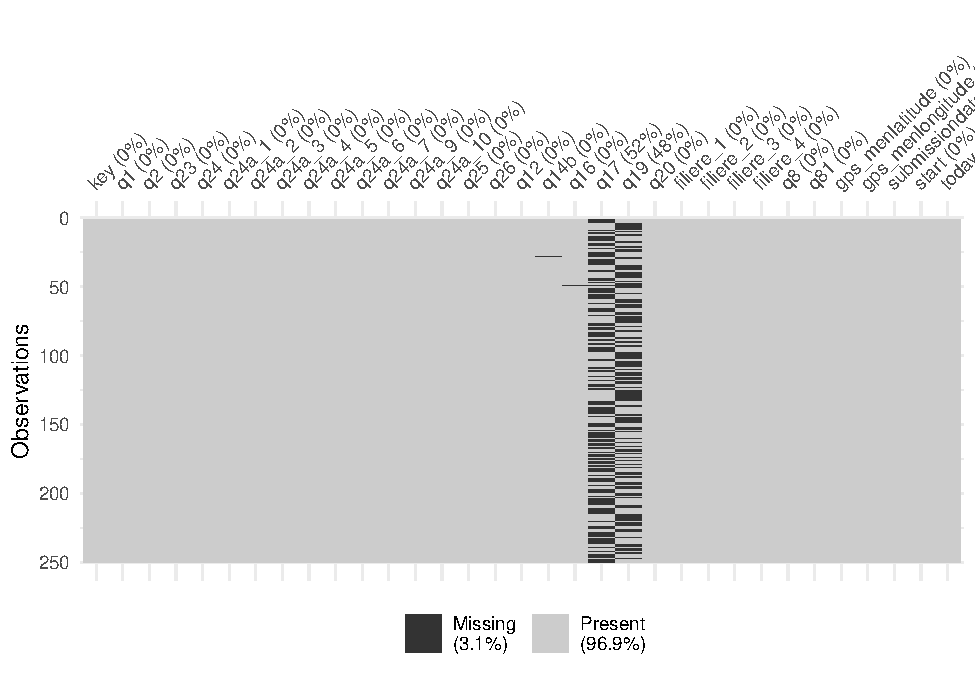
\includegraphics{Projet_R_ISE_1_files/figure-latex/unnamed-chunk-4-1} \end{center}

\hfill\break
une premiere analyse serait de se dire que les Variables labelisés
\emph{\textbf{Autorisation de fabrication et de mise en vente} et}
\emph{\textbf{L'entreprise est-elle désservie par une route bitumée ?}
ont chacune 1 valeur manquante. et que}celles labelisés* \textbf{Etat de
la route bitumée} \emph{et} \textbf{l'état de la piste qui mène à
l'entreprise} porte a elle deux près de 52\% et 48\% des valeurs
manquantes respectivement.\\
Cependant,* au regard de leur description de la base
(q17=\textbf{\emph{Etat de la route bitumée}} et
q19=\textbf{\emph{l'état de la piste qui mène à l'entreprise}})
présentent \textbf{\emph{des hors champs et non des valeurs
manquantes}}.\\

\hypertarget{pruxe9sentation-sous-forme-de-tableau-un-ruxe9sumuxe9-des-valeurs-manquantes-par-variable}{%
\paragraph{Présentation sous forme de tableau un résumé des valeurs
manquantes par
variable}\label{pruxe9sentation-sous-forme-de-tableau-un-ruxe9sumuxe9-des-valeurs-manquantes-par-variable}}

\hfill\break

\begin{Shaded}
\begin{Highlighting}[]
\NormalTok{projet }\SpecialCharTok{\%\textgreater{}\%}
          \FunctionTok{is.na}\NormalTok{() }\SpecialCharTok{\%\textgreater{}\%}                \CommentTok{\# Detection des valeurs manquantes}
          
          \FunctionTok{colSums}\NormalTok{() }\SpecialCharTok{\%\textgreater{}\%}            \CommentTok{\# sommes des valeurs par colonne}
          \FunctionTok{sort}\NormalTok{(}\AttributeTok{decreasing =} \ConstantTok{TRUE}\NormalTok{) }\SpecialCharTok{\%\textgreater{}\%} \CommentTok{\# ranger par ordre décroissant}
          
          \FunctionTok{as.data.frame}\NormalTok{() }\SpecialCharTok{\%\textgreater{}\%}
          \FunctionTok{setNames}\NormalTok{(}\StringTok{"valeurs\_manquantes"}\NormalTok{) }\SpecialCharTok{\%\textgreater{}\%}  \CommentTok{\# donner un nom à la colonne du dataframe}
          
          \FunctionTok{mutate}\NormalTok{(}\AttributeTok{pourcentage =} \FunctionTok{round}\NormalTok{(valeurs\_manquantes }\SpecialCharTok{/} \FunctionTok{sum}\NormalTok{(valeurs\_manquantes, }\AttributeTok{na.rm =} \ConstantTok{TRUE}\NormalTok{) }\SpecialCharTok{*} \DecValTok{100}\NormalTok{, }\DecValTok{2}\NormalTok{)) }\SpecialCharTok{\%\textgreater{}\%} 
        \CommentTok{\# Garder seulement les 10 premières lignes de la table}
          \FunctionTok{head}\NormalTok{(}\DecValTok{10}\NormalTok{) }\SpecialCharTok{\%\textgreater{}\%} 
        
  
          \CommentTok{\# Créer la table avec kable}
          \FunctionTok{kbl}\NormalTok{() }\SpecialCharTok{\%\textgreater{}\%}
          \FunctionTok{kable\_paper}\NormalTok{(}\AttributeTok{full\_width =} \ConstantTok{TRUE}\NormalTok{) }\SpecialCharTok{\%\textgreater{}\%}
          \FunctionTok{row\_spec}\NormalTok{(}\DecValTok{1}\SpecialCharTok{:}\DecValTok{3}\NormalTok{, }\AttributeTok{background =} \StringTok{"red"}\NormalTok{) }\SpecialCharTok{\%\textgreater{}\%} 
          \FunctionTok{row\_spec}\NormalTok{(}\DecValTok{3}\SpecialCharTok{:}\DecValTok{4}\NormalTok{, }\AttributeTok{background =} \StringTok{"blue"}\NormalTok{)}
\end{Highlighting}
\end{Shaded}

\begin{tabu} to \linewidth {>{\raggedright}X>{\raggedleft}X>{\raggedleft}X}
\hline
  & valeurs\_manquantes & pourcentage\\
\hline
\cellcolor{red}{q17} & \cellcolor{red}{131} & \cellcolor{red}{51.78}\\
\hline
\cellcolor{red}{q19} & \cellcolor{red}{120} & \cellcolor{red}{47.43}\\
\hline
\cellcolor{blue}{q14b} & \cellcolor{blue}{1} & \cellcolor{blue}{0.40}\\
\hline
\cellcolor{blue}{q16} & \cellcolor{blue}{1} & \cellcolor{blue}{0.40}\\
\hline
key & 0 & 0.00\\
\hline
q1 & 0 & 0.00\\
\hline
q2 & 0 & 0.00\\
\hline
q23 & 0 & 0.00\\
\hline
q24 & 0 & 0.00\\
\hline
q24a\_1 & 0 & 0.00\\
\hline
\end{tabu}

\hfill\break

Ce tableau vient confirmer les analyses faites plus hauts sur le concept
de valeur manquante et de hors champs.\\
\textbf{\emph{Note :}} le faite de colorier les 4 premieres lignes est
la pour faciliter la présentation des données puisque avec l'observation
graphique précédente on avait déjà une vision exhaustive de ce qui etait
cherché. Remarqu'on que le table tableaux est par ordre croissant.

\hfill\break

\hypertarget{ceci-est-le-code-dans-le-cas-ou-on-veut-afficher-tout-le-tableau}{%
\paragraph{Ceci est le code dans le cas ou on veut afficher tout le
tableau}\label{ceci-est-le-code-dans-le-cas-ou-on-veut-afficher-tout-le-tableau}}

\hfill\break

\begin{Shaded}
\begin{Highlighting}[]
 \CommentTok{\# ici c\textquotesingle{}est dans le cas ou on veut afficher toutes les variables}
\NormalTok{projet }\SpecialCharTok{\%\textgreater{}\%}
    \FunctionTok{is.na}\NormalTok{() }\SpecialCharTok{\%\textgreater{}\%}                \CommentTok{\# Detection des valeurs manquantes}
      \FunctionTok{colSums}\NormalTok{() }\SpecialCharTok{\%\textgreater{}\%}            \CommentTok{\# sommes des valeurs par colonne}
         \FunctionTok{sort}\NormalTok{(}\AttributeTok{decreasing =} \ConstantTok{TRUE}\NormalTok{) }\SpecialCharTok{\%\textgreater{}\%} \CommentTok{\# ranger par ordre décroissant}
            \FunctionTok{as.data.frame}\NormalTok{() }\SpecialCharTok{\%\textgreater{}\%}
              \FunctionTok{setNames}\NormalTok{(}\StringTok{"valeurs\_manquantes"}\NormalTok{) }\SpecialCharTok{\%\textgreater{}\%}  \CommentTok{\# donner un nom a la colonne du dataframe}
                \FunctionTok{mutate}\NormalTok{(}\AttributeTok{pourcentage =} \FunctionTok{round}\NormalTok{(valeurs\_manquantes }\SpecialCharTok{/} \FunctionTok{sum}\NormalTok{(valeurs\_manquantes, }\AttributeTok{na.rm =} \ConstantTok{TRUE}\NormalTok{) }\SpecialCharTok{*} \DecValTok{100}\NormalTok{, }\DecValTok{2}\NormalTok{)) }\SpecialCharTok{\%\textgreater{}\%}
                  \FunctionTok{kbl}\NormalTok{() }\SpecialCharTok{\%\textgreater{}\%} 
                    \FunctionTok{kable\_paper}\NormalTok{(}\AttributeTok{full\_width =} \ConstantTok{TRUE}\NormalTok{)}\SpecialCharTok{\%\textgreater{}\%}
                      \FunctionTok{row\_spec}\NormalTok{(}\DecValTok{1}\SpecialCharTok{:}\DecValTok{3}\NormalTok{, }\AttributeTok{background =} \StringTok{"red"}\NormalTok{) }\SpecialCharTok{\%\textgreater{}\%} 
                        \FunctionTok{row\_spec}\NormalTok{(}\DecValTok{3}\SpecialCharTok{:}\DecValTok{4}\NormalTok{, }\AttributeTok{background =} \StringTok{"blue"}\NormalTok{)}
\end{Highlighting}
\end{Shaded}

\begin{tabu} to \linewidth {>{\raggedright}X>{\raggedleft}X>{\raggedleft}X}
\hline
  & valeurs\_manquantes & pourcentage\\
\hline
\cellcolor{red}{q17} & \cellcolor{red}{131} & \cellcolor{red}{51.78}\\
\hline
\cellcolor{red}{q19} & \cellcolor{red}{120} & \cellcolor{red}{47.43}\\
\hline
\cellcolor{blue}{q14b} & \cellcolor{blue}{1} & \cellcolor{blue}{0.40}\\
\hline
\cellcolor{blue}{q16} & \cellcolor{blue}{1} & \cellcolor{blue}{0.40}\\
\hline
key & 0 & 0.00\\
\hline
q1 & 0 & 0.00\\
\hline
q2 & 0 & 0.00\\
\hline
q23 & 0 & 0.00\\
\hline
q24 & 0 & 0.00\\
\hline
q24a\_1 & 0 & 0.00\\
\hline
q24a\_2 & 0 & 0.00\\
\hline
q24a\_3 & 0 & 0.00\\
\hline
q24a\_4 & 0 & 0.00\\
\hline
q24a\_5 & 0 & 0.00\\
\hline
q24a\_6 & 0 & 0.00\\
\hline
q24a\_7 & 0 & 0.00\\
\hline
q24a\_9 & 0 & 0.00\\
\hline
q24a\_10 & 0 & 0.00\\
\hline
q25 & 0 & 0.00\\
\hline
q26 & 0 & 0.00\\
\hline
q12 & 0 & 0.00\\
\hline
q20 & 0 & 0.00\\
\hline
filiere\_1 & 0 & 0.00\\
\hline
filiere\_2 & 0 & 0.00\\
\hline
filiere\_3 & 0 & 0.00\\
\hline
filiere\_4 & 0 & 0.00\\
\hline
q8 & 0 & 0.00\\
\hline
q81 & 0 & 0.00\\
\hline
gps\_menlatitude & 0 & 0.00\\
\hline
gps\_menlongitude & 0 & 0.00\\
\hline
submissiondate & 0 & 0.00\\
\hline
start & 0 & 0.00\\
\hline
today & 0 & 0.00\\
\hline
\end{tabu}

\hfill\break

\hypertarget{vuxe9rification-sil-y-a-des-valeurs-manquantes-pour-la-variable-key-dans-la-base-projet.-si-cest-effectivement-le-cas-lon-identifira-la-ou-les-pme-concernuxe9es.}{%
\paragraph{Vérification s'il y a des valeurs manquantes pour la variable
key dans la base projet. Si c'est effectivement le cas , l'on identifira
la (ou les) PME
concernée(s).}\label{vuxe9rification-sil-y-a-des-valeurs-manquantes-pour-la-variable-key-dans-la-base-projet.-si-cest-effectivement-le-cas-lon-identifira-la-ou-les-pme-concernuxe9es.}}

\hfill\break

\begin{Shaded}
\begin{Highlighting}[]
\NormalTok{projet }\SpecialCharTok{\%\textgreater{}\%} 
  \FunctionTok{filter}\NormalTok{(}\FunctionTok{is.na}\NormalTok{(key)) }\SpecialCharTok{\%\textgreater{}\%}
\NormalTok{  dplyr}\SpecialCharTok{::}\FunctionTok{select}\NormalTok{(}\DecValTok{1}\SpecialCharTok{:}\DecValTok{10}\NormalTok{) }\SpecialCharTok{\%\textgreater{}\%}
       \FunctionTok{gt}\NormalTok{()}
\end{Highlighting}
\end{Shaded}

\begin{longtable}{llllrrrrrr}
\toprule
key & q1 & q2 & q23 & q24 & q24a\_1 & q24a\_2 & q24a\_3 & q24a\_4 & q24a\_5 \\ 
\midrule
\bottomrule
\end{longtable}

\hfill\break

Ce tableau vide ne fait que confirmer le resultat obtenu précédenment,
en effet la variable key n'a pas de valeurs manquantes

\textcolor{blue}{\subsubsection{Création de variables}}

\hypertarget{ruxe9nommer-les-variables-q1-en-region-q2-en-departement-et-q23-en-sexe.}{%
\paragraph{Rénommer les variables q1 en region , q2 en departement et
q23 en
sexe.}\label{ruxe9nommer-les-variables-q1-en-region-q2-en-departement-et-q23-en-sexe.}}

\hfill\break

\begin{Shaded}
\begin{Highlighting}[]
\CommentTok{\# Renommer les variables q1, q2 et q23}
\NormalTok{projet }\OtherTok{\textless{}{-}}\NormalTok{ projet }\SpecialCharTok{\%\textgreater{}\%}
              \FunctionTok{rename}\NormalTok{(}\AttributeTok{region =}\NormalTok{ q1, }\AttributeTok{departement =}\NormalTok{ q2, }\AttributeTok{sexe =}\NormalTok{ q23)}
\end{Highlighting}
\end{Shaded}

\hfill\break

\hypertarget{cruxe9er-la-variable-sexe_2-qui-vaut-1-si-sexe-uxe9gale-uxe0-femme-et-0-sinon.}{%
\paragraph{Créer la variable sexe\_2 qui vaut 1 si sexe égale à Femme et
0
sinon.}\label{cruxe9er-la-variable-sexe_2-qui-vaut-1-si-sexe-uxe9gale-uxe0-femme-et-0-sinon.}}

\hfill\break

\begin{Shaded}
\begin{Highlighting}[]
\CommentTok{\# Créer la variable sexe\_2}
\NormalTok{projet }\OtherTok{\textless{}{-}}\NormalTok{ projet }\SpecialCharTok{\%\textgreater{}\%} 
              \FunctionTok{mutate}\NormalTok{(}\AttributeTok{sexe\_2=}\FunctionTok{ifelse}\NormalTok{(projet}\SpecialCharTok{$}\NormalTok{sexe }\SpecialCharTok{==} \StringTok{"Femme"}\NormalTok{, }\DecValTok{1}\NormalTok{, }\DecValTok{0}\NormalTok{) )}
\end{Highlighting}
\end{Shaded}

\hfill\break

\hypertarget{cruxe9er-un-data.frame-nommuxe9-langues-qui-prend-les-variables-key-et-les-variables-correspondantes-duxe9crites-plus-haut.-indication-vous-remarquerez-que-ces-variables-commencent-par-q24a__.}{%
\paragraph{Créer un data.frame nommé langues qui prend les variables key
et les variables correspondantes décrites plus haut. Indication: Vous
remarquerez que ces variables commencent par
q24a\_\_.}\label{cruxe9er-un-data.frame-nommuxe9-langues-qui-prend-les-variables-key-et-les-variables-correspondantes-duxe9crites-plus-haut.-indication-vous-remarquerez-que-ces-variables-commencent-par-q24a__.}}

\hfill\break

\begin{Shaded}
\begin{Highlighting}[]
\CommentTok{\# Créer le dataframe langues }
\NormalTok{langues }\OtherTok{\textless{}{-}}\NormalTok{ projet }\SpecialCharTok{\%\textgreater{}\%}              
\NormalTok{               dplyr}\SpecialCharTok{::}\FunctionTok{select}\NormalTok{(key, }\FunctionTok{starts\_with}\NormalTok{(}\StringTok{"q24a\_"}\NormalTok{))}
\end{Highlighting}
\end{Shaded}

\hfill\break

\hypertarget{cruxe9er-une-variable-parle-qui-est-uxe9gale-au-nombre-de-langue-parluxe9e-par-le-dirigeant-de-la-pme.}{%
\paragraph{Créer une variable parle qui est égale au nombre de langue
parlée par le dirigeant de la
PME.}\label{cruxe9er-une-variable-parle-qui-est-uxe9gale-au-nombre-de-langue-parluxe9e-par-le-dirigeant-de-la-pme.}}

\hfill\break

\begin{Shaded}
\begin{Highlighting}[]
\CommentTok{\# Créer la variable "parle" en calculant la somme des réponses }
\NormalTok{langues }\OtherTok{\textless{}{-}}\NormalTok{ langues }\SpecialCharTok{\%\textgreater{}\%}                 
               \FunctionTok{mutate}\NormalTok{(}\AttributeTok{parle =} \FunctionTok{rowSums}\NormalTok{(dplyr}\SpecialCharTok{::}\FunctionTok{select}\NormalTok{(., }\FunctionTok{starts\_with}\NormalTok{(}\StringTok{"q24a\_"}\NormalTok{))))  }
\end{Highlighting}
\end{Shaded}

\hfill\break

\hypertarget{suxe9lectionnez-uniquement-les-variables-key-et-parle-lobjet-de-retour-sera-langues.}{%
\paragraph{Sélectionnez uniquement les variables key et parle, l'objet
de retour sera
langues.}\label{suxe9lectionnez-uniquement-les-variables-key-et-parle-lobjet-de-retour-sera-langues.}}

\hfill\break

\begin{Shaded}
\begin{Highlighting}[]
\NormalTok{langues }\OtherTok{\textless{}{-}}\NormalTok{ langues }\SpecialCharTok{\%\textgreater{}\%}                 
\NormalTok{                dplyr}\SpecialCharTok{::}\FunctionTok{select}\NormalTok{(key, parle)}
\end{Highlighting}
\end{Shaded}

\hfill\break

\hypertarget{merger-les-data.frame-projet-et-langues}{%
\paragraph{Merger les data.frame projet et
langues}\label{merger-les-data.frame-projet-et-langues}}

\hfill\break

\begin{Shaded}
\begin{Highlighting}[]
\NormalTok{projet}\OtherTok{\textless{}{-}}\FunctionTok{merge}\NormalTok{(projet, langues,}\AttributeTok{key\_vars=}\NormalTok{key) }
\end{Highlighting}
\end{Shaded}

\hfill\break
\ul{\textbf{Note:}} Cette partie sur la langue il etait aussi possible
de le faire en \textbf{\emph{une seule ligne de code}}. le code reduit
est donc\\

\begin{Shaded}
\begin{Highlighting}[]
\NormalTok{projet}\OtherTok{\textless{}{-}}\NormalTok{projet }\SpecialCharTok{\%\textgreater{}\%}              
           \FunctionTok{mutate}\NormalTok{(}\AttributeTok{parle2 =} \FunctionTok{rowSums}\NormalTok{(dplyr}\SpecialCharTok{::}\FunctionTok{select}\NormalTok{(., }\FunctionTok{starts\_with}\NormalTok{(}\StringTok{"q24a\_"}\NormalTok{))))}
\end{Highlighting}
\end{Shaded}

\hfill\break

\textcolor{blue}{\subsection{Analyses descriptives.}} 
\textcolor{blue}{\subsubsection{Statistiques Descriptives Univariées.}}

\hfill\break

\hypertarget{tableaux-statistiques.}{%
\paragraph{Tableaux statistiques.}\label{tableaux-statistiques.}}

\hfill\break

Quelle est la répartion des PME suivant:

\begin{itemize}
\item
  le sexe?
\item
  le niveau d'instruction?
\item
  le statut juridique?
\item
  le propriétaire/locataire?\\
\end{itemize}

\begin{Shaded}
\begin{Highlighting}[]
\CommentTok{\# Répartition des PME suivant ces variables }
\NormalTok{tab2 }\OtherTok{=}\NormalTok{  projet }\SpecialCharTok{\%\textgreater{}\%}                   
\NormalTok{           dplyr}\SpecialCharTok{::}\FunctionTok{select}\NormalTok{(sexe, q25,q12,q81) }\SpecialCharTok{\%\textgreater{}\%}                       
                \FunctionTok{rename}\NormalTok{(}\StringTok{"Niveau d’instruction du dirigeant/responsable de la PME"} \OtherTok{=}\NormalTok{ q25, }\StringTok{"Statut juridique*"}\OtherTok{=}\NormalTok{q12, }\StringTok{"*propriétaire ou locataire"}\OtherTok{=}\NormalTok{q81) }\SpecialCharTok{\%\textgreater{}\%}                                
                    \FunctionTok{tbl\_summary}\NormalTok{()}\SpecialCharTok{\%\textgreater{}\%}   
                      \FunctionTok{modify\_spanning\_header}\NormalTok{(}\FunctionTok{everything}\NormalTok{() }\SpecialCharTok{\textasciitilde{}} \StringTok{"**Répartition des PME selon les variables**"}\NormalTok{) }

\NormalTok{tab2}\SpecialCharTok{\%\textgreater{}\%} \FunctionTok{bold\_labels}\NormalTok{() }\SpecialCharTok{\%\textgreater{}\%} \CommentTok{\#Mise en forme}
              \FunctionTok{italicize\_levels}\NormalTok{()  }\SpecialCharTok{\%\textgreater{}\%}    
                    \FunctionTok{modify\_header}\NormalTok{(}\AttributeTok{update =} \FunctionTok{list}\NormalTok{( label }\SpecialCharTok{\textasciitilde{}} \StringTok{"**VARIABLE**"}\NormalTok{, }\FunctionTok{all\_stat\_cols}\NormalTok{(}\AttributeTok{stat\_0 =} \ConstantTok{FALSE}\NormalTok{) }\SpecialCharTok{\textasciitilde{}} \StringTok{"**\{level\}** (n=\{n\}, \{style\_percent(p)\}\%,size = 8)"}\NormalTok{   )) }\SpecialCharTok{\%\textgreater{}\%}
                          \FunctionTok{as\_flex\_table}\NormalTok{() }\SpecialCharTok{\%\textgreater{}\%}   
                             \FunctionTok{fontsize}\NormalTok{(}\AttributeTok{size =} \DecValTok{8}\NormalTok{) }\SpecialCharTok{\%\textgreater{}\%}   
                                \FunctionTok{width}\NormalTok{(}\AttributeTok{width =} \FloatTok{1.9}\NormalTok{)   }
\end{Highlighting}
\end{Shaded}

\global\setlength{\Oldarrayrulewidth}{\arrayrulewidth}

\global\setlength{\Oldtabcolsep}{\tabcolsep}

\setlength{\tabcolsep}{0pt}

\renewcommand*{\arraystretch}{1.5}



\providecommand{\ascline}[3]{\noalign{\global\arrayrulewidth #1}\arrayrulecolor[HTML]{#2}\cline{#3}}

\begin{longtable}[c]{|p{1.90in}|p{1.90in}}



\ascline{1pt}{000000}{1-2}

\multicolumn{2}{>{\raggedright}m{\dimexpr 3.8in+2\tabcolsep}}{\textcolor[HTML]{000000}{\fontsize{11}{11}\selectfont{\textbf{Répartition\ des\ PME\ selon\ les\ variables}}}} \\

\ascline{1pt}{000000}{1-2}



\multicolumn{1}{>{\raggedright}m{\dimexpr 1.9in+0\tabcolsep}}{\textcolor[HTML]{000000}{\fontsize{11}{11}\selectfont{\textbf{VARIABLE}}}} & \multicolumn{1}{>{\centering}m{\dimexpr 1.9in+0\tabcolsep}}{\textcolor[HTML]{000000}{\fontsize{11}{11}\selectfont{\textbf{N\ =\ 250}}}\textcolor[HTML]{000000}{\textsuperscript{\fontsize{11}{11}\selectfont{1}}}} \\

\ascline{1pt}{000000}{1-2}\endfirsthead 

\ascline{1pt}{000000}{1-2}

\multicolumn{2}{>{\raggedright}m{\dimexpr 3.8in+2\tabcolsep}}{\textcolor[HTML]{000000}{\fontsize{11}{11}\selectfont{\textbf{Répartition\ des\ PME\ selon\ les\ variables}}}} \\

\ascline{1pt}{000000}{1-2}



\multicolumn{1}{>{\raggedright}m{\dimexpr 1.9in+0\tabcolsep}}{\textcolor[HTML]{000000}{\fontsize{11}{11}\selectfont{\textbf{VARIABLE}}}} & \multicolumn{1}{>{\centering}m{\dimexpr 1.9in+0\tabcolsep}}{\textcolor[HTML]{000000}{\fontsize{11}{11}\selectfont{\textbf{N\ =\ 250}}}\textcolor[HTML]{000000}{\textsuperscript{\fontsize{11}{11}\selectfont{1}}}} \\

\ascline{1pt}{000000}{1-2}\endhead



\multicolumn{2}{>{\raggedright}m{\dimexpr 3.8in+2\tabcolsep}}{\textcolor[HTML]{000000}{\textsuperscript{\fontsize{11}{11}\selectfont{1}}}\textcolor[HTML]{000000}{\fontsize{11}{11}\selectfont{n\ (\%)}}} \\

\endfoot



\multicolumn{1}{>{\raggedright}p{\dimexpr 1.9in+0\tabcolsep}}{\textcolor[HTML]{000000}{\fontsize{8}{8}\selectfont{\textbf{sexe}}}} & \multicolumn{1}{>{\centering}p{\dimexpr 1.9in+0\tabcolsep}}{\textcolor[HTML]{000000}{\fontsize{8}{8}\selectfont{}}} \\





\multicolumn{1}{>{\raggedright}p{\dimexpr 1.9in+0\tabcolsep}}{\textcolor[HTML]{000000}{\fontsize{8}{8}\selectfont{\textit{Femme}}}} & \multicolumn{1}{>{\centering}p{\dimexpr 1.9in+0\tabcolsep}}{\textcolor[HTML]{000000}{\fontsize{8}{8}\selectfont{191\ (76\%)}}} \\





\multicolumn{1}{>{\raggedright}p{\dimexpr 1.9in+0\tabcolsep}}{\textcolor[HTML]{000000}{\fontsize{8}{8}\selectfont{\textit{Homme}}}} & \multicolumn{1}{>{\centering}p{\dimexpr 1.9in+0\tabcolsep}}{\textcolor[HTML]{000000}{\fontsize{8}{8}\selectfont{59\ (24\%)}}} \\





\multicolumn{1}{>{\raggedright}p{\dimexpr 1.9in+0\tabcolsep}}{\textcolor[HTML]{000000}{\fontsize{8}{8}\selectfont{\textbf{Niveau\ d’instruction\ du\ dirigeant/responsable\ de\ la\ PME}}}} & \multicolumn{1}{>{\centering}p{\dimexpr 1.9in+0\tabcolsep}}{\textcolor[HTML]{000000}{\fontsize{8}{8}\selectfont{}}} \\





\multicolumn{1}{>{\raggedright}p{\dimexpr 1.9in+0\tabcolsep}}{\textcolor[HTML]{000000}{\fontsize{8}{8}\selectfont{\textit{Aucun\ niveau}}}} & \multicolumn{1}{>{\centering}p{\dimexpr 1.9in+0\tabcolsep}}{\textcolor[HTML]{000000}{\fontsize{8}{8}\selectfont{79\ (32\%)}}} \\





\multicolumn{1}{>{\raggedright}p{\dimexpr 1.9in+0\tabcolsep}}{\textcolor[HTML]{000000}{\fontsize{8}{8}\selectfont{\textit{Niveau\ primaire}}}} & \multicolumn{1}{>{\centering}p{\dimexpr 1.9in+0\tabcolsep}}{\textcolor[HTML]{000000}{\fontsize{8}{8}\selectfont{56\ (22\%)}}} \\





\multicolumn{1}{>{\raggedright}p{\dimexpr 1.9in+0\tabcolsep}}{\textcolor[HTML]{000000}{\fontsize{8}{8}\selectfont{\textit{Niveau\ secondaire}}}} & \multicolumn{1}{>{\centering}p{\dimexpr 1.9in+0\tabcolsep}}{\textcolor[HTML]{000000}{\fontsize{8}{8}\selectfont{74\ (30\%)}}} \\





\multicolumn{1}{>{\raggedright}p{\dimexpr 1.9in+0\tabcolsep}}{\textcolor[HTML]{000000}{\fontsize{8}{8}\selectfont{\textit{Niveau\ Superieur}}}} & \multicolumn{1}{>{\centering}p{\dimexpr 1.9in+0\tabcolsep}}{\textcolor[HTML]{000000}{\fontsize{8}{8}\selectfont{41\ (16\%)}}} \\





\multicolumn{1}{>{\raggedright}p{\dimexpr 1.9in+0\tabcolsep}}{\textcolor[HTML]{000000}{\fontsize{8}{8}\selectfont{\textbf{Statut\ juridique*}}}} & \multicolumn{1}{>{\centering}p{\dimexpr 1.9in+0\tabcolsep}}{\textcolor[HTML]{000000}{\fontsize{8}{8}\selectfont{}}} \\





\multicolumn{1}{>{\raggedright}p{\dimexpr 1.9in+0\tabcolsep}}{\textcolor[HTML]{000000}{\fontsize{8}{8}\selectfont{\textit{Association}}}} & \multicolumn{1}{>{\centering}p{\dimexpr 1.9in+0\tabcolsep}}{\textcolor[HTML]{000000}{\fontsize{8}{8}\selectfont{6\ (2.4\%)}}} \\





\multicolumn{1}{>{\raggedright}p{\dimexpr 1.9in+0\tabcolsep}}{\textcolor[HTML]{000000}{\fontsize{8}{8}\selectfont{\textit{GIE}}}} & \multicolumn{1}{>{\centering}p{\dimexpr 1.9in+0\tabcolsep}}{\textcolor[HTML]{000000}{\fontsize{8}{8}\selectfont{179\ (72\%)}}} \\





\multicolumn{1}{>{\raggedright}p{\dimexpr 1.9in+0\tabcolsep}}{\textcolor[HTML]{000000}{\fontsize{8}{8}\selectfont{\textit{Informel}}}} & \multicolumn{1}{>{\centering}p{\dimexpr 1.9in+0\tabcolsep}}{\textcolor[HTML]{000000}{\fontsize{8}{8}\selectfont{38\ (15\%)}}} \\





\multicolumn{1}{>{\raggedright}p{\dimexpr 1.9in+0\tabcolsep}}{\textcolor[HTML]{000000}{\fontsize{8}{8}\selectfont{\textit{SA}}}} & \multicolumn{1}{>{\centering}p{\dimexpr 1.9in+0\tabcolsep}}{\textcolor[HTML]{000000}{\fontsize{8}{8}\selectfont{7\ (2.8\%)}}} \\





\multicolumn{1}{>{\raggedright}p{\dimexpr 1.9in+0\tabcolsep}}{\textcolor[HTML]{000000}{\fontsize{8}{8}\selectfont{\textit{SARL}}}} & \multicolumn{1}{>{\centering}p{\dimexpr 1.9in+0\tabcolsep}}{\textcolor[HTML]{000000}{\fontsize{8}{8}\selectfont{13\ (5.2\%)}}} \\





\multicolumn{1}{>{\raggedright}p{\dimexpr 1.9in+0\tabcolsep}}{\textcolor[HTML]{000000}{\fontsize{8}{8}\selectfont{\textit{SUARL}}}} & \multicolumn{1}{>{\centering}p{\dimexpr 1.9in+0\tabcolsep}}{\textcolor[HTML]{000000}{\fontsize{8}{8}\selectfont{7\ (2.8\%)}}} \\





\multicolumn{1}{>{\raggedright}p{\dimexpr 1.9in+0\tabcolsep}}{\textcolor[HTML]{000000}{\fontsize{8}{8}\selectfont{\textbf{*propriétaire\ ou\ locataire}}}} & \multicolumn{1}{>{\centering}p{\dimexpr 1.9in+0\tabcolsep}}{\textcolor[HTML]{000000}{\fontsize{8}{8}\selectfont{}}} \\





\multicolumn{1}{>{\raggedright}p{\dimexpr 1.9in+0\tabcolsep}}{\textcolor[HTML]{000000}{\fontsize{8}{8}\selectfont{\textit{Locataire}}}} & \multicolumn{1}{>{\centering}p{\dimexpr 1.9in+0\tabcolsep}}{\textcolor[HTML]{000000}{\fontsize{8}{8}\selectfont{24\ (9.6\%)}}} \\





\multicolumn{1}{>{\raggedright}p{\dimexpr 1.9in+0\tabcolsep}}{\textcolor[HTML]{000000}{\fontsize{8}{8}\selectfont{\textit{Propriétaire}}}} & \multicolumn{1}{>{\centering}p{\dimexpr 1.9in+0\tabcolsep}}{\textcolor[HTML]{000000}{\fontsize{8}{8}\selectfont{226\ (90\%)}}} \\

\ascline{1pt}{000000}{1-2}



\end{longtable}



\arrayrulecolor[HTML]{000000}

\global\setlength{\arrayrulewidth}{\Oldarrayrulewidth}

\global\setlength{\tabcolsep}{\Oldtabcolsep}

\renewcommand*{\arraystretch}{1}

\hfill\break

\ul{\textbf{\emph{Commentaire :}}} La plupart des PME sont dans des GIE
ou exercent dans le secteur informel. Les dirigeants des PME sont en
majorité des propriétaires, environ 90\%. On constate aussi que tres peu
d'entre eux ont un niveau supérieur .une analyse par la filière nous
donnera certainement plus de précision.\\

\hypertarget{apport-personnel}{%
\paragraph{Apport personnel}\label{apport-personnel}}

\hfill\break
Avant d'aller plus loin il est important de faire d'observer la
repartition des PME par filière :

\hfill\break

\begin{Shaded}
\begin{Highlighting}[]
\CommentTok{\# répartition des PME par filière }
\NormalTok{tab3}\OtherTok{=}\NormalTok{ projet }\SpecialCharTok{\%\textgreater{}\%}
\NormalTok{        dplyr}\SpecialCharTok{::}\FunctionTok{select}\NormalTok{(}\FunctionTok{starts\_with}\NormalTok{(}\StringTok{"filiere\_"}\NormalTok{)) }\SpecialCharTok{\%\textgreater{}\%}
  \FunctionTok{rename}\NormalTok{(}\StringTok{"arachide"}\OtherTok{=}\NormalTok{filiere\_1,}\StringTok{"Anacarde"}\OtherTok{=}\NormalTok{filiere\_2,}\StringTok{"Mangue"}\OtherTok{=}\NormalTok{filiere\_3,}\StringTok{"Riz"}\OtherTok{=}\NormalTok{filiere\_4) }\SpecialCharTok{\%\textgreater{}\%} 
              \FunctionTok{tbl\_summary}\NormalTok{( }\AttributeTok{missing =} \StringTok{"no"}\NormalTok{)}




\NormalTok{tab3}\SpecialCharTok{\%\textgreater{}\%} \FunctionTok{bold\_labels}\NormalTok{() }\SpecialCharTok{\%\textgreater{}\%} \CommentTok{\#Mise en forme}
            \FunctionTok{italicize\_levels}\NormalTok{()  }\SpecialCharTok{\%\textgreater{}\%} 
                  \FunctionTok{modify\_header}\NormalTok{(}\AttributeTok{update =} \FunctionTok{list}\NormalTok{( label }\SpecialCharTok{\textasciitilde{}} \StringTok{"**VARIABLE**"}\NormalTok{, }\FunctionTok{all\_stat\_cols}\NormalTok{(}\AttributeTok{stat\_0 =} \ConstantTok{FALSE}\NormalTok{) }\SpecialCharTok{\textasciitilde{}} \StringTok{"**\{level\}** (n=\{n\}, \{style\_percent(p)\}\%,size = 8)"}\NormalTok{   )) }\SpecialCharTok{\%\textgreater{}\%}
                    \FunctionTok{as\_flex\_table}\NormalTok{() }\SpecialCharTok{\%\textgreater{}\%}   
                          \FunctionTok{fontsize}\NormalTok{(}\AttributeTok{size =} \DecValTok{8}\NormalTok{) }\SpecialCharTok{\%\textgreater{}\%}   
                              \FunctionTok{width}\NormalTok{(}\AttributeTok{width =} \DecValTok{1}\NormalTok{) }
\end{Highlighting}
\end{Shaded}

\global\setlength{\Oldarrayrulewidth}{\arrayrulewidth}

\global\setlength{\Oldtabcolsep}{\tabcolsep}

\setlength{\tabcolsep}{0pt}

\renewcommand*{\arraystretch}{1.5}



\providecommand{\ascline}[3]{\noalign{\global\arrayrulewidth #1}\arrayrulecolor[HTML]{#2}\cline{#3}}

\begin{longtable}[c]{|p{1.00in}|p{1.00in}}



\ascline{1pt}{000000}{1-2}

\multicolumn{1}{>{\raggedright}m{\dimexpr 1in+0\tabcolsep}}{\textcolor[HTML]{000000}{\fontsize{11}{11}\selectfont{\textbf{VARIABLE}}}} & \multicolumn{1}{>{\centering}m{\dimexpr 1in+0\tabcolsep}}{\textcolor[HTML]{000000}{\fontsize{11}{11}\selectfont{\textbf{N\ =\ 250}}}\textcolor[HTML]{000000}{\textsuperscript{\fontsize{11}{11}\selectfont{1}}}} \\

\ascline{1pt}{000000}{1-2}\endfirsthead 

\ascline{1pt}{000000}{1-2}

\multicolumn{1}{>{\raggedright}m{\dimexpr 1in+0\tabcolsep}}{\textcolor[HTML]{000000}{\fontsize{11}{11}\selectfont{\textbf{VARIABLE}}}} & \multicolumn{1}{>{\centering}m{\dimexpr 1in+0\tabcolsep}}{\textcolor[HTML]{000000}{\fontsize{11}{11}\selectfont{\textbf{N\ =\ 250}}}\textcolor[HTML]{000000}{\textsuperscript{\fontsize{11}{11}\selectfont{1}}}} \\

\ascline{1pt}{000000}{1-2}\endhead



\multicolumn{2}{>{\raggedright}m{\dimexpr 2in+2\tabcolsep}}{\textcolor[HTML]{000000}{\textsuperscript{\fontsize{11}{11}\selectfont{1}}}\textcolor[HTML]{000000}{\fontsize{11}{11}\selectfont{n\ (\%)}}} \\

\endfoot



\multicolumn{1}{>{\raggedright}p{\dimexpr 1in+0\tabcolsep}}{\textcolor[HTML]{000000}{\fontsize{8}{8}\selectfont{\textbf{arachide}}}} & \multicolumn{1}{>{\centering}p{\dimexpr 1in+0\tabcolsep}}{\textcolor[HTML]{000000}{\fontsize{8}{8}\selectfont{108\ (43\%)}}} \\





\multicolumn{1}{>{\raggedright}p{\dimexpr 1in+0\tabcolsep}}{\textcolor[HTML]{000000}{\fontsize{8}{8}\selectfont{\textbf{Anacarde}}}} & \multicolumn{1}{>{\centering}p{\dimexpr 1in+0\tabcolsep}}{\textcolor[HTML]{000000}{\fontsize{8}{8}\selectfont{61\ (24\%)}}} \\





\multicolumn{1}{>{\raggedright}p{\dimexpr 1in+0\tabcolsep}}{\textcolor[HTML]{000000}{\fontsize{8}{8}\selectfont{\textbf{Mangue}}}} & \multicolumn{1}{>{\centering}p{\dimexpr 1in+0\tabcolsep}}{\textcolor[HTML]{000000}{\fontsize{8}{8}\selectfont{89\ (36\%)}}} \\





\multicolumn{1}{>{\raggedright}p{\dimexpr 1in+0\tabcolsep}}{\textcolor[HTML]{000000}{\fontsize{8}{8}\selectfont{\textbf{Riz}}}} & \multicolumn{1}{>{\centering}p{\dimexpr 1in+0\tabcolsep}}{\textcolor[HTML]{000000}{\fontsize{8}{8}\selectfont{92\ (37\%)}}} \\

\ascline{1pt}{000000}{1-2}



\end{longtable}



\arrayrulecolor[HTML]{000000}

\global\setlength{\arrayrulewidth}{\Oldarrayrulewidth}

\global\setlength{\tabcolsep}{\Oldtabcolsep}

\renewcommand*{\arraystretch}{1}

\hfill\break
La filière 1 se démarque avec la plus grande représentation, comptant
108, soit 43\% du total. Ensuite, la filière 4 suit de près avec 92,
représentant 37\%. La filière 3 occupe la troisième position avec 89 et
36\% du total, tandis que la filière 2 se trouve en quatrième position
avec 61 et 24\% du total. Ces pourcentages fournissent une vue
d'ensemble des préférences ou répartitions dans les différentes
filières, mais une analyse plus approfondie semble necessaire.

\hfill\break

Maintenant que nous savons la repartition des PME par filière, on se
demande ce qu'il en est de la répartition des PME par nombre de filière
dans laquelle agit les PME.\\

\begin{Shaded}
\begin{Highlighting}[]
\CommentTok{\# répartition des PME par nombre de filière dans laquelle agit les PME  }

\NormalTok{tab4 }\OtherTok{=}\NormalTok{ projet }\SpecialCharTok{\%\textgreater{}\%}               
  \FunctionTok{mutate}\NormalTok{(}\AttributeTok{filiere =} \FunctionTok{as.factor}\NormalTok{(}\FunctionTok{rowSums}\NormalTok{(dplyr}\SpecialCharTok{::}\FunctionTok{select}\NormalTok{(., }\FunctionTok{starts\_with}\NormalTok{(}\StringTok{"filiere\_"}\NormalTok{))))) }\SpecialCharTok{\%\textgreater{}\%}           
\NormalTok{        dplyr}\SpecialCharTok{::}\FunctionTok{select}\NormalTok{(filiere) }\SpecialCharTok{\%\textgreater{}\%}  
          \FunctionTok{rename}\NormalTok{(}\StringTok{"Nombre de filiere"}\OtherTok{=}\NormalTok{filiere) }\SpecialCharTok{\%\textgreater{}\%} 
          \FunctionTok{tbl\_summary}\NormalTok{( }\AttributeTok{missing =} \StringTok{"no"}\NormalTok{)}




\NormalTok{tab4}\SpecialCharTok{\%\textgreater{}\%} \FunctionTok{bold\_labels}\NormalTok{() }\SpecialCharTok{\%\textgreater{}\%}   \CommentTok{\#Mise en forme }
  \FunctionTok{italicize\_levels}\NormalTok{()  }\SpecialCharTok{\%\textgreater{}\%}    
    \FunctionTok{modify\_header}\NormalTok{(}\AttributeTok{update =} \FunctionTok{list}\NormalTok{( label }\SpecialCharTok{\textasciitilde{}} \StringTok{"**VARIABLE**"}\NormalTok{, }\FunctionTok{all\_stat\_cols}\NormalTok{(}\AttributeTok{stat\_0 =} \ConstantTok{FALSE}\NormalTok{) }\SpecialCharTok{\textasciitilde{}} \StringTok{"**\{level\}** (n=\{n\}, \{style\_percent(p)\}\%,size = 8)"}\NormalTok{   )) }\SpecialCharTok{\%\textgreater{}\%}  
      \FunctionTok{as\_flex\_table}\NormalTok{() }\SpecialCharTok{\%\textgreater{}\%}   
            \FunctionTok{fontsize}\NormalTok{(}\AttributeTok{size =} \DecValTok{8}\NormalTok{) }\SpecialCharTok{\%\textgreater{}\%}   
              \FunctionTok{width}\NormalTok{(}\AttributeTok{width =} \FloatTok{1.2}\NormalTok{)  }
\end{Highlighting}
\end{Shaded}

\global\setlength{\Oldarrayrulewidth}{\arrayrulewidth}

\global\setlength{\Oldtabcolsep}{\tabcolsep}

\setlength{\tabcolsep}{0pt}

\renewcommand*{\arraystretch}{1.5}



\providecommand{\ascline}[3]{\noalign{\global\arrayrulewidth #1}\arrayrulecolor[HTML]{#2}\cline{#3}}

\begin{longtable}[c]{|p{1.20in}|p{1.20in}}



\ascline{1pt}{000000}{1-2}

\multicolumn{1}{>{\raggedright}m{\dimexpr 1.2in+0\tabcolsep}}{\textcolor[HTML]{000000}{\fontsize{11}{11}\selectfont{\textbf{VARIABLE}}}} & \multicolumn{1}{>{\centering}m{\dimexpr 1.2in+0\tabcolsep}}{\textcolor[HTML]{000000}{\fontsize{11}{11}\selectfont{\textbf{N\ =\ 250}}}\textcolor[HTML]{000000}{\textsuperscript{\fontsize{11}{11}\selectfont{1}}}} \\

\ascline{1pt}{000000}{1-2}\endfirsthead 

\ascline{1pt}{000000}{1-2}

\multicolumn{1}{>{\raggedright}m{\dimexpr 1.2in+0\tabcolsep}}{\textcolor[HTML]{000000}{\fontsize{11}{11}\selectfont{\textbf{VARIABLE}}}} & \multicolumn{1}{>{\centering}m{\dimexpr 1.2in+0\tabcolsep}}{\textcolor[HTML]{000000}{\fontsize{11}{11}\selectfont{\textbf{N\ =\ 250}}}\textcolor[HTML]{000000}{\textsuperscript{\fontsize{11}{11}\selectfont{1}}}} \\

\ascline{1pt}{000000}{1-2}\endhead



\multicolumn{2}{>{\raggedright}m{\dimexpr 2.4in+2\tabcolsep}}{\textcolor[HTML]{000000}{\textsuperscript{\fontsize{11}{11}\selectfont{1}}}\textcolor[HTML]{000000}{\fontsize{11}{11}\selectfont{n\ (\%)}}} \\

\endfoot



\multicolumn{1}{>{\raggedright}p{\dimexpr 1.2in+0\tabcolsep}}{\textcolor[HTML]{000000}{\fontsize{8}{8}\selectfont{\textbf{Nombre\ de\ filiere}}}} & \multicolumn{1}{>{\centering}p{\dimexpr 1.2in+0\tabcolsep}}{\textcolor[HTML]{000000}{\fontsize{8}{8}\selectfont{}}} \\





\multicolumn{1}{>{\raggedright}p{\dimexpr 1.2in+0\tabcolsep}}{\textcolor[HTML]{000000}{\fontsize{8}{8}\selectfont{\textit{1}}}} & \multicolumn{1}{>{\centering}p{\dimexpr 1.2in+0\tabcolsep}}{\textcolor[HTML]{000000}{\fontsize{8}{8}\selectfont{171\ (68\%)}}} \\





\multicolumn{1}{>{\raggedright}p{\dimexpr 1.2in+0\tabcolsep}}{\textcolor[HTML]{000000}{\fontsize{8}{8}\selectfont{\textit{2}}}} & \multicolumn{1}{>{\centering}p{\dimexpr 1.2in+0\tabcolsep}}{\textcolor[HTML]{000000}{\fontsize{8}{8}\selectfont{59\ (24\%)}}} \\





\multicolumn{1}{>{\raggedright}p{\dimexpr 1.2in+0\tabcolsep}}{\textcolor[HTML]{000000}{\fontsize{8}{8}\selectfont{\textit{3}}}} & \multicolumn{1}{>{\centering}p{\dimexpr 1.2in+0\tabcolsep}}{\textcolor[HTML]{000000}{\fontsize{8}{8}\selectfont{19\ (7.6\%)}}} \\





\multicolumn{1}{>{\raggedright}p{\dimexpr 1.2in+0\tabcolsep}}{\textcolor[HTML]{000000}{\fontsize{8}{8}\selectfont{\textit{4}}}} & \multicolumn{1}{>{\centering}p{\dimexpr 1.2in+0\tabcolsep}}{\textcolor[HTML]{000000}{\fontsize{8}{8}\selectfont{1\ (0.4\%)}}} \\

\ascline{1pt}{000000}{1-2}



\end{longtable}



\arrayrulecolor[HTML]{000000}

\global\setlength{\arrayrulewidth}{\Oldarrayrulewidth}

\global\setlength{\tabcolsep}{\Oldtabcolsep}

\renewcommand*{\arraystretch}{1}

\hfill\break
il ressort d'une analyse rapide que certains entreprises sont dans
plusieurs filière à la fois. En effet \textbf{79} sont celles qui sont
dans au moins une filière. L'analyse approfondie nous révèle que
\textbf{59} d'entre elles sont dans deux ilières et une seule est dans
quatre filières.\\
\strut \\

\hypertarget{cruxe9ation-dune-variable-avec-le-nom-des-filiuxe8res.}{%
\subparagraph{Création d'une variable avec le nom des
filières.}\label{cruxe9ation-dune-variable-avec-le-nom-des-filiuxe8res.}}

\hfill\break
Cette variable est crée pour faire des séparations stricte sur les
filières, ceci dans l'optique de distinguer les PME qui sont dans
plusieurs activités.\\

\hfill\break

\hypertarget{ruxe9pruxe9sentation-graphique.}{%
\subparagraph{Réprésentation
graphique.}\label{ruxe9pruxe9sentation-graphique.}}

\hfill\break

-Répartition des PME selon le sexe, le niveau scolaire, le statut
juridique et le type du dirigeant

\hfill\break
Une réprésentation graphique semble intéressante pour observer ses
variables.\\

\begin{Shaded}
\begin{Highlighting}[]
\CommentTok{\# Sélection des PME selon le sexe, le niveau scolaire,}
\CommentTok{\#le statut juridique et le type du dirigeant}
\NormalTok{pme\_repartition }\OtherTok{\textless{}{-}}\NormalTok{ projet }\SpecialCharTok{\%\textgreater{}\%}
\NormalTok{  dplyr}\SpecialCharTok{::}\FunctionTok{select}\NormalTok{(sexe, q25, q12, q81)}

\CommentTok{\# Créer les graphiques en secteurs pleins avec les pourcentages}
\NormalTok{plot1 }\OtherTok{\textless{}{-}} \FunctionTok{ggplot}\NormalTok{(pme\_repartition }\SpecialCharTok{\%\textgreater{}\%}
                 \FunctionTok{count}\NormalTok{(sexe) }\SpecialCharTok{\%\textgreater{}\%}
                 \FunctionTok{mutate}\NormalTok{(}\AttributeTok{percentage =}\NormalTok{ n }\SpecialCharTok{/} \FunctionTok{sum}\NormalTok{(n) }\SpecialCharTok{*} \DecValTok{100}\NormalTok{), }
                \FunctionTok{aes}\NormalTok{(}\AttributeTok{x =} \StringTok{""}\NormalTok{, }\AttributeTok{y =}\NormalTok{ percentage, }\AttributeTok{fill =}\NormalTok{ sexe)) }\SpecialCharTok{+}
  \FunctionTok{geom\_bar}\NormalTok{(}\AttributeTok{stat =} \StringTok{"identity"}\NormalTok{, }\AttributeTok{position =} \StringTok{"fill"}\NormalTok{) }\SpecialCharTok{+}
  \FunctionTok{coord\_polar}\NormalTok{(}\StringTok{"y"}\NormalTok{) }\SpecialCharTok{+}
  \FunctionTok{scale\_fill\_manual}\NormalTok{(}\AttributeTok{values =} \FunctionTok{c}\NormalTok{(}\StringTok{"\#E45756"}\NormalTok{, }\StringTok{"\#4C78A8"}\NormalTok{)) }\SpecialCharTok{+}
  \FunctionTok{labs}\NormalTok{(}\AttributeTok{x =} \ConstantTok{NULL}\NormalTok{, }\AttributeTok{y =} \ConstantTok{NULL}\NormalTok{, }\AttributeTok{fill =} \StringTok{"SEXE"}\NormalTok{) }\SpecialCharTok{+}
  \FunctionTok{geom\_text}\NormalTok{(}\FunctionTok{aes}\NormalTok{(}\AttributeTok{label =} \FunctionTok{paste0}\NormalTok{(}\FunctionTok{round}\NormalTok{(percentage, }\DecValTok{1}\NormalTok{), }\StringTok{"\%"}\NormalTok{)), }
            \AttributeTok{position =} \FunctionTok{position\_fill}\NormalTok{(}\AttributeTok{vjust =} \FloatTok{0.5}\NormalTok{), }\AttributeTok{color =} \StringTok{"white"}\NormalTok{,}\AttributeTok{size =} \DecValTok{3}\NormalTok{) }\SpecialCharTok{+}
  \FunctionTok{theme\_classic}\NormalTok{() }\SpecialCharTok{+}
  \FunctionTok{theme}\NormalTok{(}\AttributeTok{plot.title =} \FunctionTok{element\_text}\NormalTok{(}\AttributeTok{size =} \DecValTok{8}\NormalTok{, }\AttributeTok{hjust =} \FloatTok{0.5}\NormalTok{)) }


\NormalTok{plot2 }\OtherTok{\textless{}{-}} \FunctionTok{ggplot}\NormalTok{(pme\_repartition }\SpecialCharTok{\%\textgreater{}\%}
                 \FunctionTok{count}\NormalTok{(q25) }\SpecialCharTok{\%\textgreater{}\%}
                 \FunctionTok{mutate}\NormalTok{(}\AttributeTok{percentage =}\NormalTok{ n }\SpecialCharTok{/} \FunctionTok{sum}\NormalTok{(n) }\SpecialCharTok{*} \DecValTok{100}\NormalTok{), }
                \FunctionTok{aes}\NormalTok{(}\AttributeTok{x =} \StringTok{""}\NormalTok{, }\AttributeTok{y =}\NormalTok{ percentage, }\AttributeTok{fill =}\NormalTok{ q25)) }\SpecialCharTok{+}
  \FunctionTok{geom\_bar}\NormalTok{(}\AttributeTok{stat =} \StringTok{"identity"}\NormalTok{, }\AttributeTok{position =} \StringTok{"fill"}\NormalTok{) }\SpecialCharTok{+}
  \FunctionTok{coord\_polar}\NormalTok{(}\StringTok{"y"}\NormalTok{) }\SpecialCharTok{+}
  \FunctionTok{scale\_fill\_manual}\NormalTok{(}\AttributeTok{values =} \FunctionTok{c}\NormalTok{(}\StringTok{"\#E45756"}\NormalTok{, }\StringTok{"\#4C78A8"}\NormalTok{, }\StringTok{"darkgreen"}\NormalTok{, }\StringTok{"blue"}\NormalTok{)) }\SpecialCharTok{+}
  \FunctionTok{labs}\NormalTok{(}\AttributeTok{x =} \ConstantTok{NULL}\NormalTok{, }\AttributeTok{y =} \ConstantTok{NULL}\NormalTok{, }\AttributeTok{fill =} \StringTok{"NIVEAU ACADEMIQUE"}\NormalTok{) }\SpecialCharTok{+}
  \FunctionTok{geom\_text}\NormalTok{(}\FunctionTok{aes}\NormalTok{(}\AttributeTok{label =} \FunctionTok{paste0}\NormalTok{(}\FunctionTok{round}\NormalTok{(percentage, }\DecValTok{1}\NormalTok{), }\StringTok{"\%"}\NormalTok{)), }
            \AttributeTok{position =} \FunctionTok{position\_fill}\NormalTok{(}\AttributeTok{vjust =} \FloatTok{0.5}\NormalTok{), }\AttributeTok{color =} \StringTok{"white"}\NormalTok{,}\AttributeTok{size =} \DecValTok{3}\NormalTok{) }\SpecialCharTok{+}
  \FunctionTok{theme\_classic}\NormalTok{() }\SpecialCharTok{+}
  \FunctionTok{theme}\NormalTok{(}\AttributeTok{plot.title =} \FunctionTok{element\_text}\NormalTok{(}\AttributeTok{size =} \DecValTok{12}\NormalTok{, }\AttributeTok{hjust =} \FloatTok{0.5}\NormalTok{))}

\NormalTok{plot3 }\OtherTok{\textless{}{-}} \FunctionTok{ggplot}\NormalTok{(pme\_repartition }\SpecialCharTok{\%\textgreater{}\%}
                 \FunctionTok{count}\NormalTok{(q12) }\SpecialCharTok{\%\textgreater{}\%}
                 \FunctionTok{mutate}\NormalTok{(}\AttributeTok{percentage =}\NormalTok{ n }\SpecialCharTok{/} \FunctionTok{sum}\NormalTok{(n) }\SpecialCharTok{*} \DecValTok{100}\NormalTok{),}
                \FunctionTok{aes}\NormalTok{(}\AttributeTok{x =} \StringTok{""}\NormalTok{, }\AttributeTok{y =}\NormalTok{ n, }\AttributeTok{fill =}\NormalTok{ q12)) }\SpecialCharTok{+}
  \FunctionTok{geom\_bar}\NormalTok{(}\AttributeTok{stat =} \StringTok{"identity"}\NormalTok{) }\SpecialCharTok{+}
  \FunctionTok{scale\_fill\_manual}\NormalTok{(}\AttributeTok{values =} \FunctionTok{c}\NormalTok{(}\StringTok{"\#E45756"}\NormalTok{, }\StringTok{"\#4C78A8"}\NormalTok{, }
                               \StringTok{"darkgreen"}\NormalTok{, }\StringTok{"blue"}\NormalTok{, }\StringTok{"pink"}\NormalTok{, }\StringTok{"lightgreen"}\NormalTok{)) }\SpecialCharTok{+}
  \FunctionTok{labs}\NormalTok{(}\AttributeTok{x =} \ConstantTok{NULL}\NormalTok{, }\AttributeTok{y =} \ConstantTok{NULL}\NormalTok{, }\AttributeTok{fill =} \StringTok{"STATUT JURIDIQUE"}\NormalTok{) }\SpecialCharTok{+}
  \FunctionTok{geom\_text}\NormalTok{(}\FunctionTok{aes}\NormalTok{(}\AttributeTok{label =} \FunctionTok{paste0}\NormalTok{(}\FunctionTok{round}\NormalTok{(percentage, }\DecValTok{1}\NormalTok{), }\StringTok{"\%"}\NormalTok{)), }
            \AttributeTok{position =} \FunctionTok{position\_stack}\NormalTok{(}\AttributeTok{vjust =} \FloatTok{0.5}\NormalTok{), }\AttributeTok{color =} \StringTok{"white"}\NormalTok{,}\AttributeTok{size =} \DecValTok{3}\NormalTok{) }\SpecialCharTok{+}
  \FunctionTok{theme\_classic}\NormalTok{() }\SpecialCharTok{+}
  \FunctionTok{theme}\NormalTok{(}\AttributeTok{plot.title =} \FunctionTok{element\_text}\NormalTok{(}\AttributeTok{size =} \DecValTok{8}\NormalTok{, }\AttributeTok{hjust =} \FloatTok{0.5}\NormalTok{))}

\NormalTok{plot4 }\OtherTok{\textless{}{-}} \FunctionTok{ggplot}\NormalTok{(pme\_repartition }\SpecialCharTok{\%\textgreater{}\%}
                 \FunctionTok{count}\NormalTok{(q81) }\SpecialCharTok{\%\textgreater{}\%}
                 \FunctionTok{mutate}\NormalTok{(}\AttributeTok{percentage =}\NormalTok{ n }\SpecialCharTok{/} \FunctionTok{sum}\NormalTok{(n) }\SpecialCharTok{*} \DecValTok{100}\NormalTok{), }
                \FunctionTok{aes}\NormalTok{(}\AttributeTok{x =} \StringTok{""}\NormalTok{, }\AttributeTok{y =}\NormalTok{ percentage, }\AttributeTok{fill =}\NormalTok{ q81)) }\SpecialCharTok{+}
  \FunctionTok{geom\_bar}\NormalTok{(}\AttributeTok{stat =} \StringTok{"identity"}\NormalTok{, }\AttributeTok{position =} \StringTok{"fill"}\NormalTok{) }\SpecialCharTok{+}
  \FunctionTok{coord\_polar}\NormalTok{(}\StringTok{"y"}\NormalTok{) }\SpecialCharTok{+}
  \FunctionTok{scale\_fill\_manual}\NormalTok{(}\AttributeTok{values =} \FunctionTok{c}\NormalTok{(}\StringTok{"\#E45756"}\NormalTok{, }\StringTok{"\#4C78A8"}\NormalTok{)) }\SpecialCharTok{+}
  \FunctionTok{labs}\NormalTok{(}\AttributeTok{x =} \ConstantTok{NULL}\NormalTok{, }\AttributeTok{y =} \ConstantTok{NULL}\NormalTok{, }\AttributeTok{fill =} \StringTok{"PROP/LOCA"}\NormalTok{) }\SpecialCharTok{+}
  \FunctionTok{geom\_text}\NormalTok{(}\FunctionTok{aes}\NormalTok{(}\AttributeTok{label =} \FunctionTok{paste0}\NormalTok{(}\FunctionTok{round}\NormalTok{(percentage, }\DecValTok{1}\NormalTok{), }\StringTok{"\%"}\NormalTok{)), }
            \AttributeTok{position =} \FunctionTok{position\_fill}\NormalTok{(}\AttributeTok{vjust =} \FloatTok{0.5}\NormalTok{), }\AttributeTok{color =} \StringTok{"white"}\NormalTok{,}\AttributeTok{size =} \DecValTok{3}\NormalTok{) }\SpecialCharTok{+}
  \FunctionTok{theme\_classic}\NormalTok{() }\SpecialCharTok{+}
  \FunctionTok{theme}\NormalTok{(}\AttributeTok{plot.title =} \FunctionTok{element\_text}\NormalTok{(}\AttributeTok{size =} \DecValTok{12}\NormalTok{, }\AttributeTok{hjust =} \FloatTok{0.5}\NormalTok{))}
\CommentTok{\# Personnaliser le thème global}
\NormalTok{custom\_theme }\OtherTok{\textless{}{-}} \FunctionTok{theme}\NormalTok{(}
  \AttributeTok{plot.margin =} \FunctionTok{unit}\NormalTok{(}\FunctionTok{c}\NormalTok{(}\DecValTok{1}\NormalTok{, }\DecValTok{1}\NormalTok{, }\DecValTok{1}\NormalTok{, }\DecValTok{1}\NormalTok{), }\StringTok{"lines"}\NormalTok{),}
  \AttributeTok{axis.text =} \FunctionTok{element\_blank}\NormalTok{(),}
  \AttributeTok{axis.ticks =} \FunctionTok{element\_blank}\NormalTok{(),}
  \AttributeTok{legend.title =} \FunctionTok{element\_text}\NormalTok{(}\AttributeTok{size =} \DecValTok{10}\NormalTok{, }\AttributeTok{face =} \StringTok{"bold"}\NormalTok{),}
  \AttributeTok{legend.text =} \FunctionTok{element\_text}\NormalTok{(}\AttributeTok{size =} \DecValTok{8}\NormalTok{),}
  \AttributeTok{legend.key.size =} \FunctionTok{unit}\NormalTok{(}\FloatTok{0.5}\NormalTok{, }\StringTok{"lines"}\NormalTok{),}
  \AttributeTok{legend.key =} \FunctionTok{element\_rect}\NormalTok{(}\AttributeTok{color =} \StringTok{"transparent"}\NormalTok{),}
  \AttributeTok{panel.spacing =} \FunctionTok{unit}\NormalTok{(}\DecValTok{3}\NormalTok{, }\StringTok{"lines"}\NormalTok{)}
\NormalTok{)}
\CommentTok{\# Afficher les 4 graphiques côte à côte avec le thème }
\CommentTok{\#personnalisé et des barres de séparation}
\FunctionTok{grid.arrange}\NormalTok{(plot1 }\SpecialCharTok{+}\NormalTok{ custom\_theme, plot2 }\SpecialCharTok{+}\NormalTok{ custom\_theme, }
\NormalTok{             plot3 }\SpecialCharTok{+}\NormalTok{ custom\_theme, plot4 }\SpecialCharTok{+}\NormalTok{ custom\_theme, }
             \AttributeTok{ncol =} \DecValTok{2}\NormalTok{, }\AttributeTok{nrow =} \DecValTok{2}\NormalTok{, }\AttributeTok{widths =} \FunctionTok{c}\NormalTok{(}\DecValTok{1}\NormalTok{, }\DecValTok{1}\NormalTok{), }\AttributeTok{heights =} \FunctionTok{c}\NormalTok{(}\DecValTok{1}\NormalTok{, }\DecValTok{1}\NormalTok{), }
             \AttributeTok{top =} \StringTok{"REPARTITION DES PME SELON }
\StringTok{             LES CARACTERISTIQUES DES DIRIGEANTS"}\NormalTok{)}
\end{Highlighting}
\end{Shaded}

\begin{center}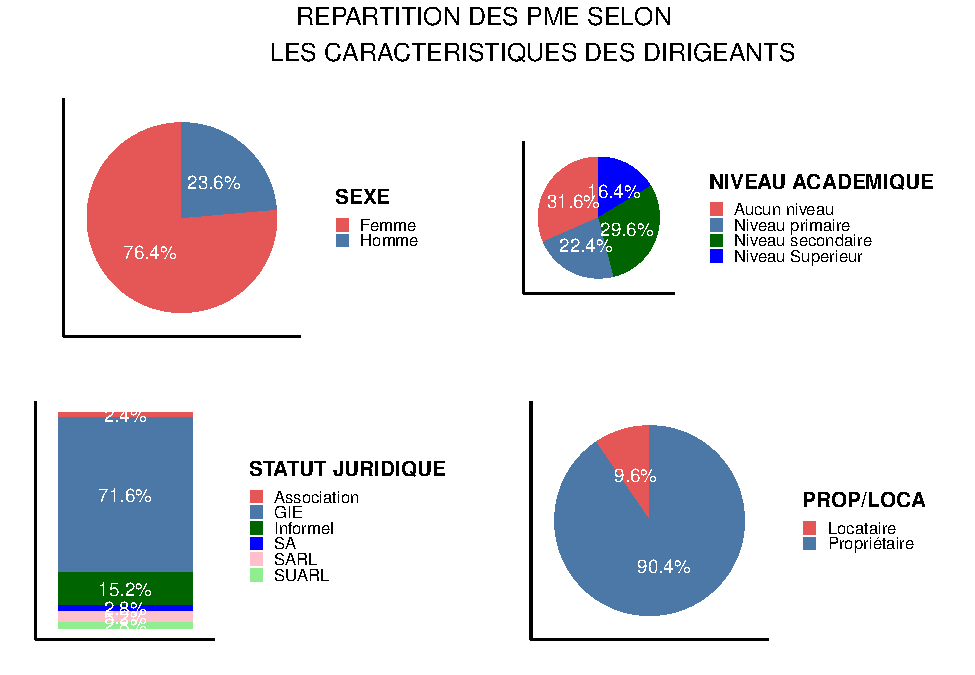
\includegraphics{Projet_R_ISE_1_files/figure-latex/unnamed-chunk-19-1} \end{center}

\hfill\break

\textcolor{blue}{\subsubsection{ Statistiques descriptives bivariées.}}

\hfill\break

\hypertarget{tableaux-statistiques.-1}{%
\paragraph{Tableaux statistiques.}\label{tableaux-statistiques.-1}}

\hfill\break
- le statut juridique et le sexe

\begin{itemize}
\item
  Niveau d'instruction du dirigeant/responsable de la PME et sexe
\item
  propriétaire ou locataire et sexe
\end{itemize}

\hfill\break

\begin{Shaded}
\begin{Highlighting}[]
\CommentTok{\# Répartition selon le statut juridique et le sexe,Niveau }
\CommentTok{\#d\textquotesingle{}instruction du dirigeant/responsable de la PME et sexe, }
\CommentTok{\#propriétaire ou locataire et sexe : profil colonne}

\NormalTok{tab}\OtherTok{=}\NormalTok{projet }\SpecialCharTok{\%\textgreater{}\%}
\NormalTok{         dplyr}\SpecialCharTok{::}\FunctionTok{select}\NormalTok{(q81,q25,q12, sexe) }\SpecialCharTok{\%\textgreater{}\%}
           \FunctionTok{rename}\NormalTok{(}\StringTok{"Niveau d’instruction du dirigeant/responsable de la PME"} \OtherTok{=}\NormalTok{ q25, }
             \StringTok{"Statut juridique*"}\OtherTok{=}\NormalTok{q12, }\StringTok{"propriétaire ou locataire"}\OtherTok{=}\NormalTok{q81) }\SpecialCharTok{\%\textgreater{}\%} 
                \FunctionTok{tbl\_summary}\NormalTok{(}\AttributeTok{by =}\NormalTok{ sexe, }\AttributeTok{missing =} \StringTok{"no"}\NormalTok{)}\SpecialCharTok{\%\textgreater{}\%}
                  \FunctionTok{modify\_spanning\_header}\NormalTok{(}\FunctionTok{everything}\NormalTok{() }\SpecialCharTok{\textasciitilde{}} \StringTok{"**Répartition }
\StringTok{                  des PME selonleur statut juridique }
\StringTok{                                         et le sexe de son dirigeant**"}\NormalTok{)}
\NormalTok{tab}\SpecialCharTok{\%\textgreater{}\%} \FunctionTok{bold\_labels}\NormalTok{() }\SpecialCharTok{\%\textgreater{}\%}    \CommentTok{\#Mise en forme}
  \FunctionTok{italicize\_levels}\NormalTok{()  }\SpecialCharTok{\%\textgreater{}\%}    
      \FunctionTok{modify\_header}\NormalTok{(}\AttributeTok{update =} \FunctionTok{list}\NormalTok{( label }\SpecialCharTok{\textasciitilde{}} \StringTok{"**VARIABLE**"}\NormalTok{, }
                                   \FunctionTok{all\_stat\_cols}\NormalTok{(}\AttributeTok{stat\_0 =} \ConstantTok{FALSE}\NormalTok{) }\SpecialCharTok{\textasciitilde{}} \StringTok{"**\{level\}**}
\StringTok{                                   (n=\{n\}, \{style\_percent(p)\}\%)"}\NormalTok{   )) }\SpecialCharTok{\%\textgreater{}\%}  
          \FunctionTok{as\_flex\_table}\NormalTok{() }\SpecialCharTok{\%\textgreater{}\%}   
        \FunctionTok{fontsize}\NormalTok{(}\AttributeTok{size =} \DecValTok{8}\NormalTok{) }\SpecialCharTok{\%\textgreater{}\%}   
            \FunctionTok{width}\NormalTok{(}\AttributeTok{width =} \FloatTok{1.7}\NormalTok{)  }
\end{Highlighting}
\end{Shaded}

\global\setlength{\Oldarrayrulewidth}{\arrayrulewidth}

\global\setlength{\Oldtabcolsep}{\tabcolsep}

\setlength{\tabcolsep}{0pt}

\renewcommand*{\arraystretch}{1.5}



\providecommand{\ascline}[3]{\noalign{\global\arrayrulewidth #1}\arrayrulecolor[HTML]{#2}\cline{#3}}

\begin{longtable}[c]{|p{1.70in}|p{1.70in}|p{1.70in}}



\ascline{1pt}{000000}{1-3}

\multicolumn{3}{>{\raggedright}m{\dimexpr 5.1in+4\tabcolsep}}{\textcolor[HTML]{000000}{\fontsize{11}{11}\selectfont{\textbf{**Répartition\ }}}\textcolor[HTML]{000000}{\fontsize{11}{11}\selectfont{\textbf{\linebreak }}}\textcolor[HTML]{000000}{\fontsize{11}{11}\selectfont{\textbf{des\ PME\ selonleur\ statut\ juridique\ }}}\textcolor[HTML]{000000}{\fontsize{11}{11}\selectfont{\textbf{\linebreak }}}\textcolor[HTML]{000000}{\fontsize{11}{11}\selectfont{\textbf{\ \ \ \ \ \ \ \ \ \ \ \ \ \ \ \ \ \ \ \ \ \ \ et\ le\ sexe\ de\ son\ dirigeant**}}}} \\

\ascline{1pt}{000000}{1-3}



\multicolumn{1}{>{\raggedright}m{\dimexpr 1.7in+0\tabcolsep}}{\textcolor[HTML]{000000}{\fontsize{11}{11}\selectfont{\textbf{VARIABLE}}}} & \multicolumn{1}{>{\centering}m{\dimexpr 1.7in+0\tabcolsep}}{\textcolor[HTML]{000000}{\fontsize{11}{11}\selectfont{\textbf{Femme}}}\textcolor[HTML]{000000}{\fontsize{11}{11}\selectfont{\linebreak }}\textcolor[HTML]{000000}{\fontsize{11}{11}\selectfont{(n=191,\ 76\%)}}\textcolor[HTML]{000000}{\textsuperscript{\fontsize{11}{11}\selectfont{1}}}} & \multicolumn{1}{>{\centering}m{\dimexpr 1.7in+0\tabcolsep}}{\textcolor[HTML]{000000}{\fontsize{11}{11}\selectfont{\textbf{Homme}}}\textcolor[HTML]{000000}{\fontsize{11}{11}\selectfont{\linebreak }}\textcolor[HTML]{000000}{\fontsize{11}{11}\selectfont{(n=59,\ 24\%)}}\textcolor[HTML]{000000}{\textsuperscript{\fontsize{11}{11}\selectfont{1}}}} \\

\ascline{1pt}{000000}{1-3}\endfirsthead 

\ascline{1pt}{000000}{1-3}

\multicolumn{3}{>{\raggedright}m{\dimexpr 5.1in+4\tabcolsep}}{\textcolor[HTML]{000000}{\fontsize{11}{11}\selectfont{\textbf{**Répartition\ }}}\textcolor[HTML]{000000}{\fontsize{11}{11}\selectfont{\textbf{\linebreak }}}\textcolor[HTML]{000000}{\fontsize{11}{11}\selectfont{\textbf{des\ PME\ selonleur\ statut\ juridique\ }}}\textcolor[HTML]{000000}{\fontsize{11}{11}\selectfont{\textbf{\linebreak }}}\textcolor[HTML]{000000}{\fontsize{11}{11}\selectfont{\textbf{\ \ \ \ \ \ \ \ \ \ \ \ \ \ \ \ \ \ \ \ \ \ \ et\ le\ sexe\ de\ son\ dirigeant**}}}} \\

\ascline{1pt}{000000}{1-3}



\multicolumn{1}{>{\raggedright}m{\dimexpr 1.7in+0\tabcolsep}}{\textcolor[HTML]{000000}{\fontsize{11}{11}\selectfont{\textbf{VARIABLE}}}} & \multicolumn{1}{>{\centering}m{\dimexpr 1.7in+0\tabcolsep}}{\textcolor[HTML]{000000}{\fontsize{11}{11}\selectfont{\textbf{Femme}}}\textcolor[HTML]{000000}{\fontsize{11}{11}\selectfont{\linebreak }}\textcolor[HTML]{000000}{\fontsize{11}{11}\selectfont{(n=191,\ 76\%)}}\textcolor[HTML]{000000}{\textsuperscript{\fontsize{11}{11}\selectfont{1}}}} & \multicolumn{1}{>{\centering}m{\dimexpr 1.7in+0\tabcolsep}}{\textcolor[HTML]{000000}{\fontsize{11}{11}\selectfont{\textbf{Homme}}}\textcolor[HTML]{000000}{\fontsize{11}{11}\selectfont{\linebreak }}\textcolor[HTML]{000000}{\fontsize{11}{11}\selectfont{(n=59,\ 24\%)}}\textcolor[HTML]{000000}{\textsuperscript{\fontsize{11}{11}\selectfont{1}}}} \\

\ascline{1pt}{000000}{1-3}\endhead



\multicolumn{3}{>{\raggedright}m{\dimexpr 5.1in+4\tabcolsep}}{\textcolor[HTML]{000000}{\textsuperscript{\fontsize{11}{11}\selectfont{1}}}\textcolor[HTML]{000000}{\fontsize{11}{11}\selectfont{n\ (\%)}}} \\

\endfoot



\multicolumn{1}{>{\raggedright}p{\dimexpr 1.7in+0\tabcolsep}}{\textcolor[HTML]{000000}{\fontsize{8}{8}\selectfont{\textbf{propriétaire\ ou\ locataire}}}} & \multicolumn{1}{>{\centering}p{\dimexpr 1.7in+0\tabcolsep}}{\textcolor[HTML]{000000}{\fontsize{8}{8}\selectfont{}}} & \multicolumn{1}{>{\centering}p{\dimexpr 1.7in+0\tabcolsep}}{\textcolor[HTML]{000000}{\fontsize{8}{8}\selectfont{}}} \\





\multicolumn{1}{>{\raggedright}p{\dimexpr 1.7in+0\tabcolsep}}{\textcolor[HTML]{000000}{\fontsize{8}{8}\selectfont{\textit{Locataire}}}} & \multicolumn{1}{>{\centering}p{\dimexpr 1.7in+0\tabcolsep}}{\textcolor[HTML]{000000}{\fontsize{8}{8}\selectfont{16\ (8.4\%)}}} & \multicolumn{1}{>{\centering}p{\dimexpr 1.7in+0\tabcolsep}}{\textcolor[HTML]{000000}{\fontsize{8}{8}\selectfont{8\ (14\%)}}} \\





\multicolumn{1}{>{\raggedright}p{\dimexpr 1.7in+0\tabcolsep}}{\textcolor[HTML]{000000}{\fontsize{8}{8}\selectfont{\textit{Propriétaire}}}} & \multicolumn{1}{>{\centering}p{\dimexpr 1.7in+0\tabcolsep}}{\textcolor[HTML]{000000}{\fontsize{8}{8}\selectfont{175\ (92\%)}}} & \multicolumn{1}{>{\centering}p{\dimexpr 1.7in+0\tabcolsep}}{\textcolor[HTML]{000000}{\fontsize{8}{8}\selectfont{51\ (86\%)}}} \\





\multicolumn{1}{>{\raggedright}p{\dimexpr 1.7in+0\tabcolsep}}{\textcolor[HTML]{000000}{\fontsize{8}{8}\selectfont{\textbf{Niveau\ d’instruction\ du\ dirigeant/responsable\ de\ la\ PME}}}} & \multicolumn{1}{>{\centering}p{\dimexpr 1.7in+0\tabcolsep}}{\textcolor[HTML]{000000}{\fontsize{8}{8}\selectfont{}}} & \multicolumn{1}{>{\centering}p{\dimexpr 1.7in+0\tabcolsep}}{\textcolor[HTML]{000000}{\fontsize{8}{8}\selectfont{}}} \\





\multicolumn{1}{>{\raggedright}p{\dimexpr 1.7in+0\tabcolsep}}{\textcolor[HTML]{000000}{\fontsize{8}{8}\selectfont{\textit{Aucun\ niveau}}}} & \multicolumn{1}{>{\centering}p{\dimexpr 1.7in+0\tabcolsep}}{\textcolor[HTML]{000000}{\fontsize{8}{8}\selectfont{70\ (37\%)}}} & \multicolumn{1}{>{\centering}p{\dimexpr 1.7in+0\tabcolsep}}{\textcolor[HTML]{000000}{\fontsize{8}{8}\selectfont{9\ (15\%)}}} \\





\multicolumn{1}{>{\raggedright}p{\dimexpr 1.7in+0\tabcolsep}}{\textcolor[HTML]{000000}{\fontsize{8}{8}\selectfont{\textit{Niveau\ primaire}}}} & \multicolumn{1}{>{\centering}p{\dimexpr 1.7in+0\tabcolsep}}{\textcolor[HTML]{000000}{\fontsize{8}{8}\selectfont{48\ (25\%)}}} & \multicolumn{1}{>{\centering}p{\dimexpr 1.7in+0\tabcolsep}}{\textcolor[HTML]{000000}{\fontsize{8}{8}\selectfont{8\ (14\%)}}} \\





\multicolumn{1}{>{\raggedright}p{\dimexpr 1.7in+0\tabcolsep}}{\textcolor[HTML]{000000}{\fontsize{8}{8}\selectfont{\textit{Niveau\ secondaire}}}} & \multicolumn{1}{>{\centering}p{\dimexpr 1.7in+0\tabcolsep}}{\textcolor[HTML]{000000}{\fontsize{8}{8}\selectfont{56\ (29\%)}}} & \multicolumn{1}{>{\centering}p{\dimexpr 1.7in+0\tabcolsep}}{\textcolor[HTML]{000000}{\fontsize{8}{8}\selectfont{18\ (31\%)}}} \\





\multicolumn{1}{>{\raggedright}p{\dimexpr 1.7in+0\tabcolsep}}{\textcolor[HTML]{000000}{\fontsize{8}{8}\selectfont{\textit{Niveau\ Superieur}}}} & \multicolumn{1}{>{\centering}p{\dimexpr 1.7in+0\tabcolsep}}{\textcolor[HTML]{000000}{\fontsize{8}{8}\selectfont{17\ (8.9\%)}}} & \multicolumn{1}{>{\centering}p{\dimexpr 1.7in+0\tabcolsep}}{\textcolor[HTML]{000000}{\fontsize{8}{8}\selectfont{24\ (41\%)}}} \\





\multicolumn{1}{>{\raggedright}p{\dimexpr 1.7in+0\tabcolsep}}{\textcolor[HTML]{000000}{\fontsize{8}{8}\selectfont{\textbf{Statut\ juridique*}}}} & \multicolumn{1}{>{\centering}p{\dimexpr 1.7in+0\tabcolsep}}{\textcolor[HTML]{000000}{\fontsize{8}{8}\selectfont{}}} & \multicolumn{1}{>{\centering}p{\dimexpr 1.7in+0\tabcolsep}}{\textcolor[HTML]{000000}{\fontsize{8}{8}\selectfont{}}} \\





\multicolumn{1}{>{\raggedright}p{\dimexpr 1.7in+0\tabcolsep}}{\textcolor[HTML]{000000}{\fontsize{8}{8}\selectfont{\textit{Association}}}} & \multicolumn{1}{>{\centering}p{\dimexpr 1.7in+0\tabcolsep}}{\textcolor[HTML]{000000}{\fontsize{8}{8}\selectfont{3\ (1.6\%)}}} & \multicolumn{1}{>{\centering}p{\dimexpr 1.7in+0\tabcolsep}}{\textcolor[HTML]{000000}{\fontsize{8}{8}\selectfont{3\ (5.1\%)}}} \\





\multicolumn{1}{>{\raggedright}p{\dimexpr 1.7in+0\tabcolsep}}{\textcolor[HTML]{000000}{\fontsize{8}{8}\selectfont{\textit{GIE}}}} & \multicolumn{1}{>{\centering}p{\dimexpr 1.7in+0\tabcolsep}}{\textcolor[HTML]{000000}{\fontsize{8}{8}\selectfont{149\ (78\%)}}} & \multicolumn{1}{>{\centering}p{\dimexpr 1.7in+0\tabcolsep}}{\textcolor[HTML]{000000}{\fontsize{8}{8}\selectfont{30\ (51\%)}}} \\





\multicolumn{1}{>{\raggedright}p{\dimexpr 1.7in+0\tabcolsep}}{\textcolor[HTML]{000000}{\fontsize{8}{8}\selectfont{\textit{Informel}}}} & \multicolumn{1}{>{\centering}p{\dimexpr 1.7in+0\tabcolsep}}{\textcolor[HTML]{000000}{\fontsize{8}{8}\selectfont{32\ (17\%)}}} & \multicolumn{1}{>{\centering}p{\dimexpr 1.7in+0\tabcolsep}}{\textcolor[HTML]{000000}{\fontsize{8}{8}\selectfont{6\ (10\%)}}} \\





\multicolumn{1}{>{\raggedright}p{\dimexpr 1.7in+0\tabcolsep}}{\textcolor[HTML]{000000}{\fontsize{8}{8}\selectfont{\textit{SA}}}} & \multicolumn{1}{>{\centering}p{\dimexpr 1.7in+0\tabcolsep}}{\textcolor[HTML]{000000}{\fontsize{8}{8}\selectfont{1\ (0.5\%)}}} & \multicolumn{1}{>{\centering}p{\dimexpr 1.7in+0\tabcolsep}}{\textcolor[HTML]{000000}{\fontsize{8}{8}\selectfont{6\ (10\%)}}} \\





\multicolumn{1}{>{\raggedright}p{\dimexpr 1.7in+0\tabcolsep}}{\textcolor[HTML]{000000}{\fontsize{8}{8}\selectfont{\textit{SARL}}}} & \multicolumn{1}{>{\centering}p{\dimexpr 1.7in+0\tabcolsep}}{\textcolor[HTML]{000000}{\fontsize{8}{8}\selectfont{2\ (1.0\%)}}} & \multicolumn{1}{>{\centering}p{\dimexpr 1.7in+0\tabcolsep}}{\textcolor[HTML]{000000}{\fontsize{8}{8}\selectfont{11\ (19\%)}}} \\





\multicolumn{1}{>{\raggedright}p{\dimexpr 1.7in+0\tabcolsep}}{\textcolor[HTML]{000000}{\fontsize{8}{8}\selectfont{\textit{SUARL}}}} & \multicolumn{1}{>{\centering}p{\dimexpr 1.7in+0\tabcolsep}}{\textcolor[HTML]{000000}{\fontsize{8}{8}\selectfont{4\ (2.1\%)}}} & \multicolumn{1}{>{\centering}p{\dimexpr 1.7in+0\tabcolsep}}{\textcolor[HTML]{000000}{\fontsize{8}{8}\selectfont{3\ (5.1\%)}}} \\

\ascline{1pt}{000000}{1-3}



\end{longtable}



\arrayrulecolor[HTML]{000000}

\global\setlength{\arrayrulewidth}{\Oldarrayrulewidth}

\global\setlength{\tabcolsep}{\Oldtabcolsep}

\renewcommand*{\arraystretch}{1}

\hfill\break

\ul{\textbf{\emph{Commentaire:}}}~

Parmi les propriétaires, 92\% sont des femmes, tandis que parmi les
locataires, la répartition est plus équilibrée avec 14\% de femmes et
14\% d'hommes.

En ce qui concerne le niveau d'éducation, les hommes ont tendance à
avoir un niveau d'éducation supérieur (41\%) par rapport aux femmes
(8,9\%).

Par contre, les femmes ont une plus grande présence dans les niveaux
d'éducation primaire (14\%) et secondaire (29\%) par rapport aux hommes
(14\% et 31\% respectivement).

on constate que les entreprises dirigées par des hommes ont une plus
grande présence dans les formes juridiques de type GIE (Groupement
d'Intérêt Économique), SA (Société Anonyme), SARL (Société à
Responsabilité Limitée) et SUARL (Société Unipersonnelle à
Responsabilité Limitée).

D'autre part, les femmes dirigeantes dominent dans le statut juridique
informel, qui représente 17\% de leur part, tandis que les hommes n'en
représentent que 10\%.

\hfill\break

\hypertarget{faire-en-sortir-les-statistiques-univariuxe9es-et-bivariuxe9es-en-un-seul-tableau}{%
\paragraph{Faire en sortir les statistiques univariées et Bivariées en
un seul
tableau}\label{faire-en-sortir-les-statistiques-univariuxe9es-et-bivariuxe9es-en-un-seul-tableau}}

\hfill\break

\begin{Shaded}
\begin{Highlighting}[]
\FunctionTok{tbl\_merge}\NormalTok{(}\FunctionTok{list}\NormalTok{(tab2,tab),}
           \CommentTok{\# definition des panels}
          \AttributeTok{tab\_spanner =} \FunctionTok{c}\NormalTok{(}\StringTok{"ANALYSE UNIVARIE"}\NormalTok{,}
                                         \StringTok{"ANALYSE BIVARIE"}\NormalTok{))}\SpecialCharTok{\%\textgreater{}\%}
  
  \CommentTok{\# Mise en forme}
  \CommentTok{\# Mise en Gras}
  \FunctionTok{bold\_labels}\NormalTok{() }\SpecialCharTok{\%\textgreater{}\%} 
  
  
  \CommentTok{\# Mise en italique}
  \FunctionTok{italicize\_levels}\NormalTok{()  }\SpecialCharTok{\%\textgreater{}\%} 
  
  \CommentTok{\# Mise en forme des entêtes}
  
  \FunctionTok{modify\_header}\NormalTok{(}\AttributeTok{update =} \FunctionTok{list}\NormalTok{( label }\SpecialCharTok{\textasciitilde{}} \StringTok{"**VARIABLE**"}\NormalTok{, }
                               \FunctionTok{all\_stat\_cols}\NormalTok{(}\AttributeTok{stat\_0 =} \ConstantTok{FALSE}\NormalTok{) }\SpecialCharTok{\textasciitilde{}} \StringTok{"**\{level\}**}
\StringTok{                               (n=\{n\},\{style\_percent(p)\}\%)"}\NormalTok{))                                              }\SpecialCharTok{\%\textgreater{}\%} 
                                 \FunctionTok{as\_flex\_table}\NormalTok{() }\SpecialCharTok{\%\textgreater{}\%}
                               \CommentTok{\# Mise en forme des dimensions}
                                 \FunctionTok{fontsize}\NormalTok{(}\AttributeTok{size =} \DecValTok{8}\NormalTok{) }\SpecialCharTok{\%\textgreater{}\%}
                                 \FunctionTok{width}\NormalTok{(}\AttributeTok{width =} \FloatTok{1.65}\NormalTok{)}
\end{Highlighting}
\end{Shaded}

\global\setlength{\Oldarrayrulewidth}{\arrayrulewidth}

\global\setlength{\Oldtabcolsep}{\tabcolsep}

\setlength{\tabcolsep}{0pt}

\renewcommand*{\arraystretch}{1.5}



\providecommand{\ascline}[3]{\noalign{\global\arrayrulewidth #1}\arrayrulecolor[HTML]{#2}\cline{#3}}

\begin{longtable}[c]{|p{1.65in}|p{1.65in}|p{1.65in}|p{1.65in}}



\ascline{1pt}{000000}{1-4}

\multicolumn{1}{>{\raggedright}m{\dimexpr 1.65in+0\tabcolsep}}{\textcolor[HTML]{000000}{\fontsize{11}{11}\selectfont{\textbf{Répartition\ des\ PME\ selon\ les\ variables}}}} & \multicolumn{1}{>{\centering}m{\dimexpr 1.65in+0\tabcolsep}}{\textcolor[HTML]{000000}{\fontsize{11}{11}\selectfont{ANALYSE\ UNIVARIE}}} & \multicolumn{2}{>{\centering}m{\dimexpr 3.3in+2\tabcolsep}}{\textcolor[HTML]{000000}{\fontsize{11}{11}\selectfont{ANALYSE\ BIVARIE}}} \\

\ascline{1pt}{000000}{1-4}



\multicolumn{1}{>{\raggedright}m{\dimexpr 1.65in+0\tabcolsep}}{\textcolor[HTML]{000000}{\fontsize{11}{11}\selectfont{\textbf{VARIABLE}}}} & \multicolumn{1}{>{\centering}m{\dimexpr 1.65in+0\tabcolsep}}{\textcolor[HTML]{000000}{\fontsize{11}{11}\selectfont{\textbf{N\ =\ 250}}}\textcolor[HTML]{000000}{\textsuperscript{\fontsize{11}{11}\selectfont{1}}}} & \multicolumn{1}{>{\centering}m{\dimexpr 1.65in+0\tabcolsep}}{\textcolor[HTML]{000000}{\fontsize{11}{11}\selectfont{\textbf{Femme}}}\textcolor[HTML]{000000}{\fontsize{11}{11}\selectfont{\linebreak }}\textcolor[HTML]{000000}{\fontsize{11}{11}\selectfont{(n=191,76\%)}}\textcolor[HTML]{000000}{\textsuperscript{\fontsize{11}{11}\selectfont{1}}}} & \multicolumn{1}{>{\centering}m{\dimexpr 1.65in+0\tabcolsep}}{\textcolor[HTML]{000000}{\fontsize{11}{11}\selectfont{\textbf{Homme}}}\textcolor[HTML]{000000}{\fontsize{11}{11}\selectfont{\linebreak }}\textcolor[HTML]{000000}{\fontsize{11}{11}\selectfont{(n=59,24\%)}}\textcolor[HTML]{000000}{\textsuperscript{\fontsize{11}{11}\selectfont{1}}}} \\

\ascline{1pt}{000000}{1-4}\endfirsthead 

\ascline{1pt}{000000}{1-4}

\multicolumn{1}{>{\raggedright}m{\dimexpr 1.65in+0\tabcolsep}}{\textcolor[HTML]{000000}{\fontsize{11}{11}\selectfont{\textbf{Répartition\ des\ PME\ selon\ les\ variables}}}} & \multicolumn{1}{>{\centering}m{\dimexpr 1.65in+0\tabcolsep}}{\textcolor[HTML]{000000}{\fontsize{11}{11}\selectfont{ANALYSE\ UNIVARIE}}} & \multicolumn{2}{>{\centering}m{\dimexpr 3.3in+2\tabcolsep}}{\textcolor[HTML]{000000}{\fontsize{11}{11}\selectfont{ANALYSE\ BIVARIE}}} \\

\ascline{1pt}{000000}{1-4}



\multicolumn{1}{>{\raggedright}m{\dimexpr 1.65in+0\tabcolsep}}{\textcolor[HTML]{000000}{\fontsize{11}{11}\selectfont{\textbf{VARIABLE}}}} & \multicolumn{1}{>{\centering}m{\dimexpr 1.65in+0\tabcolsep}}{\textcolor[HTML]{000000}{\fontsize{11}{11}\selectfont{\textbf{N\ =\ 250}}}\textcolor[HTML]{000000}{\textsuperscript{\fontsize{11}{11}\selectfont{1}}}} & \multicolumn{1}{>{\centering}m{\dimexpr 1.65in+0\tabcolsep}}{\textcolor[HTML]{000000}{\fontsize{11}{11}\selectfont{\textbf{Femme}}}\textcolor[HTML]{000000}{\fontsize{11}{11}\selectfont{\linebreak }}\textcolor[HTML]{000000}{\fontsize{11}{11}\selectfont{(n=191,76\%)}}\textcolor[HTML]{000000}{\textsuperscript{\fontsize{11}{11}\selectfont{1}}}} & \multicolumn{1}{>{\centering}m{\dimexpr 1.65in+0\tabcolsep}}{\textcolor[HTML]{000000}{\fontsize{11}{11}\selectfont{\textbf{Homme}}}\textcolor[HTML]{000000}{\fontsize{11}{11}\selectfont{\linebreak }}\textcolor[HTML]{000000}{\fontsize{11}{11}\selectfont{(n=59,24\%)}}\textcolor[HTML]{000000}{\textsuperscript{\fontsize{11}{11}\selectfont{1}}}} \\

\ascline{1pt}{000000}{1-4}\endhead



\multicolumn{4}{>{\raggedright}m{\dimexpr 6.6in+6\tabcolsep}}{\textcolor[HTML]{000000}{\textsuperscript{\fontsize{11}{11}\selectfont{1}}}\textcolor[HTML]{000000}{\fontsize{11}{11}\selectfont{n\ (\%)}}} \\

\endfoot



\multicolumn{1}{>{\raggedright}p{\dimexpr 1.65in+0\tabcolsep}}{\textcolor[HTML]{000000}{\fontsize{8}{8}\selectfont{\textbf{sexe}}}} & \multicolumn{1}{>{\centering}p{\dimexpr 1.65in+0\tabcolsep}}{\textcolor[HTML]{000000}{\fontsize{8}{8}\selectfont{}}} & \multicolumn{1}{>{\centering}p{\dimexpr 1.65in+0\tabcolsep}}{\textcolor[HTML]{000000}{\fontsize{8}{8}\selectfont{}}} & \multicolumn{1}{>{\centering}p{\dimexpr 1.65in+0\tabcolsep}}{\textcolor[HTML]{000000}{\fontsize{8}{8}\selectfont{}}} \\





\multicolumn{1}{>{\raggedright}p{\dimexpr 1.65in+0\tabcolsep}}{\textcolor[HTML]{000000}{\fontsize{8}{8}\selectfont{\textit{Femme}}}} & \multicolumn{1}{>{\centering}p{\dimexpr 1.65in+0\tabcolsep}}{\textcolor[HTML]{000000}{\fontsize{8}{8}\selectfont{191\ (76\%)}}} & \multicolumn{1}{>{\centering}p{\dimexpr 1.65in+0\tabcolsep}}{\textcolor[HTML]{000000}{\fontsize{8}{8}\selectfont{}}} & \multicolumn{1}{>{\centering}p{\dimexpr 1.65in+0\tabcolsep}}{\textcolor[HTML]{000000}{\fontsize{8}{8}\selectfont{}}} \\





\multicolumn{1}{>{\raggedright}p{\dimexpr 1.65in+0\tabcolsep}}{\textcolor[HTML]{000000}{\fontsize{8}{8}\selectfont{\textit{Homme}}}} & \multicolumn{1}{>{\centering}p{\dimexpr 1.65in+0\tabcolsep}}{\textcolor[HTML]{000000}{\fontsize{8}{8}\selectfont{59\ (24\%)}}} & \multicolumn{1}{>{\centering}p{\dimexpr 1.65in+0\tabcolsep}}{\textcolor[HTML]{000000}{\fontsize{8}{8}\selectfont{}}} & \multicolumn{1}{>{\centering}p{\dimexpr 1.65in+0\tabcolsep}}{\textcolor[HTML]{000000}{\fontsize{8}{8}\selectfont{}}} \\





\multicolumn{1}{>{\raggedright}p{\dimexpr 1.65in+0\tabcolsep}}{\textcolor[HTML]{000000}{\fontsize{8}{8}\selectfont{\textbf{Niveau\ d’instruction\ du\ dirigeant/responsable\ de\ la\ PME}}}} & \multicolumn{1}{>{\centering}p{\dimexpr 1.65in+0\tabcolsep}}{\textcolor[HTML]{000000}{\fontsize{8}{8}\selectfont{}}} & \multicolumn{1}{>{\centering}p{\dimexpr 1.65in+0\tabcolsep}}{\textcolor[HTML]{000000}{\fontsize{8}{8}\selectfont{}}} & \multicolumn{1}{>{\centering}p{\dimexpr 1.65in+0\tabcolsep}}{\textcolor[HTML]{000000}{\fontsize{8}{8}\selectfont{}}} \\





\multicolumn{1}{>{\raggedright}p{\dimexpr 1.65in+0\tabcolsep}}{\textcolor[HTML]{000000}{\fontsize{8}{8}\selectfont{\textit{Aucun\ niveau}}}} & \multicolumn{1}{>{\centering}p{\dimexpr 1.65in+0\tabcolsep}}{\textcolor[HTML]{000000}{\fontsize{8}{8}\selectfont{79\ (32\%)}}} & \multicolumn{1}{>{\centering}p{\dimexpr 1.65in+0\tabcolsep}}{\textcolor[HTML]{000000}{\fontsize{8}{8}\selectfont{70\ (37\%)}}} & \multicolumn{1}{>{\centering}p{\dimexpr 1.65in+0\tabcolsep}}{\textcolor[HTML]{000000}{\fontsize{8}{8}\selectfont{9\ (15\%)}}} \\





\multicolumn{1}{>{\raggedright}p{\dimexpr 1.65in+0\tabcolsep}}{\textcolor[HTML]{000000}{\fontsize{8}{8}\selectfont{\textit{Niveau\ primaire}}}} & \multicolumn{1}{>{\centering}p{\dimexpr 1.65in+0\tabcolsep}}{\textcolor[HTML]{000000}{\fontsize{8}{8}\selectfont{56\ (22\%)}}} & \multicolumn{1}{>{\centering}p{\dimexpr 1.65in+0\tabcolsep}}{\textcolor[HTML]{000000}{\fontsize{8}{8}\selectfont{48\ (25\%)}}} & \multicolumn{1}{>{\centering}p{\dimexpr 1.65in+0\tabcolsep}}{\textcolor[HTML]{000000}{\fontsize{8}{8}\selectfont{8\ (14\%)}}} \\





\multicolumn{1}{>{\raggedright}p{\dimexpr 1.65in+0\tabcolsep}}{\textcolor[HTML]{000000}{\fontsize{8}{8}\selectfont{\textit{Niveau\ secondaire}}}} & \multicolumn{1}{>{\centering}p{\dimexpr 1.65in+0\tabcolsep}}{\textcolor[HTML]{000000}{\fontsize{8}{8}\selectfont{74\ (30\%)}}} & \multicolumn{1}{>{\centering}p{\dimexpr 1.65in+0\tabcolsep}}{\textcolor[HTML]{000000}{\fontsize{8}{8}\selectfont{56\ (29\%)}}} & \multicolumn{1}{>{\centering}p{\dimexpr 1.65in+0\tabcolsep}}{\textcolor[HTML]{000000}{\fontsize{8}{8}\selectfont{18\ (31\%)}}} \\





\multicolumn{1}{>{\raggedright}p{\dimexpr 1.65in+0\tabcolsep}}{\textcolor[HTML]{000000}{\fontsize{8}{8}\selectfont{\textit{Niveau\ Superieur}}}} & \multicolumn{1}{>{\centering}p{\dimexpr 1.65in+0\tabcolsep}}{\textcolor[HTML]{000000}{\fontsize{8}{8}\selectfont{41\ (16\%)}}} & \multicolumn{1}{>{\centering}p{\dimexpr 1.65in+0\tabcolsep}}{\textcolor[HTML]{000000}{\fontsize{8}{8}\selectfont{17\ (8.9\%)}}} & \multicolumn{1}{>{\centering}p{\dimexpr 1.65in+0\tabcolsep}}{\textcolor[HTML]{000000}{\fontsize{8}{8}\selectfont{24\ (41\%)}}} \\





\multicolumn{1}{>{\raggedright}p{\dimexpr 1.65in+0\tabcolsep}}{\textcolor[HTML]{000000}{\fontsize{8}{8}\selectfont{\textbf{Statut\ juridique*}}}} & \multicolumn{1}{>{\centering}p{\dimexpr 1.65in+0\tabcolsep}}{\textcolor[HTML]{000000}{\fontsize{8}{8}\selectfont{}}} & \multicolumn{1}{>{\centering}p{\dimexpr 1.65in+0\tabcolsep}}{\textcolor[HTML]{000000}{\fontsize{8}{8}\selectfont{}}} & \multicolumn{1}{>{\centering}p{\dimexpr 1.65in+0\tabcolsep}}{\textcolor[HTML]{000000}{\fontsize{8}{8}\selectfont{}}} \\





\multicolumn{1}{>{\raggedright}p{\dimexpr 1.65in+0\tabcolsep}}{\textcolor[HTML]{000000}{\fontsize{8}{8}\selectfont{\textit{Association}}}} & \multicolumn{1}{>{\centering}p{\dimexpr 1.65in+0\tabcolsep}}{\textcolor[HTML]{000000}{\fontsize{8}{8}\selectfont{6\ (2.4\%)}}} & \multicolumn{1}{>{\centering}p{\dimexpr 1.65in+0\tabcolsep}}{\textcolor[HTML]{000000}{\fontsize{8}{8}\selectfont{3\ (1.6\%)}}} & \multicolumn{1}{>{\centering}p{\dimexpr 1.65in+0\tabcolsep}}{\textcolor[HTML]{000000}{\fontsize{8}{8}\selectfont{3\ (5.1\%)}}} \\





\multicolumn{1}{>{\raggedright}p{\dimexpr 1.65in+0\tabcolsep}}{\textcolor[HTML]{000000}{\fontsize{8}{8}\selectfont{\textit{GIE}}}} & \multicolumn{1}{>{\centering}p{\dimexpr 1.65in+0\tabcolsep}}{\textcolor[HTML]{000000}{\fontsize{8}{8}\selectfont{179\ (72\%)}}} & \multicolumn{1}{>{\centering}p{\dimexpr 1.65in+0\tabcolsep}}{\textcolor[HTML]{000000}{\fontsize{8}{8}\selectfont{149\ (78\%)}}} & \multicolumn{1}{>{\centering}p{\dimexpr 1.65in+0\tabcolsep}}{\textcolor[HTML]{000000}{\fontsize{8}{8}\selectfont{30\ (51\%)}}} \\





\multicolumn{1}{>{\raggedright}p{\dimexpr 1.65in+0\tabcolsep}}{\textcolor[HTML]{000000}{\fontsize{8}{8}\selectfont{\textit{Informel}}}} & \multicolumn{1}{>{\centering}p{\dimexpr 1.65in+0\tabcolsep}}{\textcolor[HTML]{000000}{\fontsize{8}{8}\selectfont{38\ (15\%)}}} & \multicolumn{1}{>{\centering}p{\dimexpr 1.65in+0\tabcolsep}}{\textcolor[HTML]{000000}{\fontsize{8}{8}\selectfont{32\ (17\%)}}} & \multicolumn{1}{>{\centering}p{\dimexpr 1.65in+0\tabcolsep}}{\textcolor[HTML]{000000}{\fontsize{8}{8}\selectfont{6\ (10\%)}}} \\





\multicolumn{1}{>{\raggedright}p{\dimexpr 1.65in+0\tabcolsep}}{\textcolor[HTML]{000000}{\fontsize{8}{8}\selectfont{\textit{SA}}}} & \multicolumn{1}{>{\centering}p{\dimexpr 1.65in+0\tabcolsep}}{\textcolor[HTML]{000000}{\fontsize{8}{8}\selectfont{7\ (2.8\%)}}} & \multicolumn{1}{>{\centering}p{\dimexpr 1.65in+0\tabcolsep}}{\textcolor[HTML]{000000}{\fontsize{8}{8}\selectfont{1\ (0.5\%)}}} & \multicolumn{1}{>{\centering}p{\dimexpr 1.65in+0\tabcolsep}}{\textcolor[HTML]{000000}{\fontsize{8}{8}\selectfont{6\ (10\%)}}} \\





\multicolumn{1}{>{\raggedright}p{\dimexpr 1.65in+0\tabcolsep}}{\textcolor[HTML]{000000}{\fontsize{8}{8}\selectfont{\textit{SARL}}}} & \multicolumn{1}{>{\centering}p{\dimexpr 1.65in+0\tabcolsep}}{\textcolor[HTML]{000000}{\fontsize{8}{8}\selectfont{13\ (5.2\%)}}} & \multicolumn{1}{>{\centering}p{\dimexpr 1.65in+0\tabcolsep}}{\textcolor[HTML]{000000}{\fontsize{8}{8}\selectfont{2\ (1.0\%)}}} & \multicolumn{1}{>{\centering}p{\dimexpr 1.65in+0\tabcolsep}}{\textcolor[HTML]{000000}{\fontsize{8}{8}\selectfont{11\ (19\%)}}} \\





\multicolumn{1}{>{\raggedright}p{\dimexpr 1.65in+0\tabcolsep}}{\textcolor[HTML]{000000}{\fontsize{8}{8}\selectfont{\textit{SUARL}}}} & \multicolumn{1}{>{\centering}p{\dimexpr 1.65in+0\tabcolsep}}{\textcolor[HTML]{000000}{\fontsize{8}{8}\selectfont{7\ (2.8\%)}}} & \multicolumn{1}{>{\centering}p{\dimexpr 1.65in+0\tabcolsep}}{\textcolor[HTML]{000000}{\fontsize{8}{8}\selectfont{4\ (2.1\%)}}} & \multicolumn{1}{>{\centering}p{\dimexpr 1.65in+0\tabcolsep}}{\textcolor[HTML]{000000}{\fontsize{8}{8}\selectfont{3\ (5.1\%)}}} \\





\multicolumn{1}{>{\raggedright}p{\dimexpr 1.65in+0\tabcolsep}}{\textcolor[HTML]{000000}{\fontsize{8}{8}\selectfont{\textbf{*propriétaire\ ou\ locataire}}}} & \multicolumn{1}{>{\centering}p{\dimexpr 1.65in+0\tabcolsep}}{\textcolor[HTML]{000000}{\fontsize{8}{8}\selectfont{}}} & \multicolumn{1}{>{\centering}p{\dimexpr 1.65in+0\tabcolsep}}{\textcolor[HTML]{000000}{\fontsize{8}{8}\selectfont{}}} & \multicolumn{1}{>{\centering}p{\dimexpr 1.65in+0\tabcolsep}}{\textcolor[HTML]{000000}{\fontsize{8}{8}\selectfont{}}} \\





\multicolumn{1}{>{\raggedright}p{\dimexpr 1.65in+0\tabcolsep}}{\textcolor[HTML]{000000}{\fontsize{8}{8}\selectfont{\textit{Locataire}}}} & \multicolumn{1}{>{\centering}p{\dimexpr 1.65in+0\tabcolsep}}{\textcolor[HTML]{000000}{\fontsize{8}{8}\selectfont{24\ (9.6\%)}}} & \multicolumn{1}{>{\centering}p{\dimexpr 1.65in+0\tabcolsep}}{\textcolor[HTML]{000000}{\fontsize{8}{8}\selectfont{}}} & \multicolumn{1}{>{\centering}p{\dimexpr 1.65in+0\tabcolsep}}{\textcolor[HTML]{000000}{\fontsize{8}{8}\selectfont{}}} \\





\multicolumn{1}{>{\raggedright}p{\dimexpr 1.65in+0\tabcolsep}}{\textcolor[HTML]{000000}{\fontsize{8}{8}\selectfont{\textit{Propriétaire}}}} & \multicolumn{1}{>{\centering}p{\dimexpr 1.65in+0\tabcolsep}}{\textcolor[HTML]{000000}{\fontsize{8}{8}\selectfont{226\ (90\%)}}} & \multicolumn{1}{>{\centering}p{\dimexpr 1.65in+0\tabcolsep}}{\textcolor[HTML]{000000}{\fontsize{8}{8}\selectfont{}}} & \multicolumn{1}{>{\centering}p{\dimexpr 1.65in+0\tabcolsep}}{\textcolor[HTML]{000000}{\fontsize{8}{8}\selectfont{}}} \\





\multicolumn{1}{>{\raggedright}p{\dimexpr 1.65in+0\tabcolsep}}{\textcolor[HTML]{000000}{\fontsize{8}{8}\selectfont{\textbf{propriétaire\ ou\ locataire}}}} & \multicolumn{1}{>{\centering}p{\dimexpr 1.65in+0\tabcolsep}}{\textcolor[HTML]{000000}{\fontsize{8}{8}\selectfont{}}} & \multicolumn{1}{>{\centering}p{\dimexpr 1.65in+0\tabcolsep}}{\textcolor[HTML]{000000}{\fontsize{8}{8}\selectfont{}}} & \multicolumn{1}{>{\centering}p{\dimexpr 1.65in+0\tabcolsep}}{\textcolor[HTML]{000000}{\fontsize{8}{8}\selectfont{}}} \\





\multicolumn{1}{>{\raggedright}p{\dimexpr 1.65in+0\tabcolsep}}{\textcolor[HTML]{000000}{\fontsize{8}{8}\selectfont{\textit{Locataire}}}} & \multicolumn{1}{>{\centering}p{\dimexpr 1.65in+0\tabcolsep}}{\textcolor[HTML]{000000}{\fontsize{8}{8}\selectfont{}}} & \multicolumn{1}{>{\centering}p{\dimexpr 1.65in+0\tabcolsep}}{\textcolor[HTML]{000000}{\fontsize{8}{8}\selectfont{16\ (8.4\%)}}} & \multicolumn{1}{>{\centering}p{\dimexpr 1.65in+0\tabcolsep}}{\textcolor[HTML]{000000}{\fontsize{8}{8}\selectfont{8\ (14\%)}}} \\





\multicolumn{1}{>{\raggedright}p{\dimexpr 1.65in+0\tabcolsep}}{\textcolor[HTML]{000000}{\fontsize{8}{8}\selectfont{\textit{Propriétaire}}}} & \multicolumn{1}{>{\centering}p{\dimexpr 1.65in+0\tabcolsep}}{\textcolor[HTML]{000000}{\fontsize{8}{8}\selectfont{}}} & \multicolumn{1}{>{\centering}p{\dimexpr 1.65in+0\tabcolsep}}{\textcolor[HTML]{000000}{\fontsize{8}{8}\selectfont{175\ (92\%)}}} & \multicolumn{1}{>{\centering}p{\dimexpr 1.65in+0\tabcolsep}}{\textcolor[HTML]{000000}{\fontsize{8}{8}\selectfont{51\ (86\%)}}} \\

\ascline{1pt}{000000}{1-4}



\end{longtable}



\arrayrulecolor[HTML]{000000}

\global\setlength{\arrayrulewidth}{\Oldarrayrulewidth}

\global\setlength{\tabcolsep}{\Oldtabcolsep}

\renewcommand*{\arraystretch}{1}

\hfill\break

\hypertarget{ruxe9presentation-graphique}{%
\paragraph{Répresentation graphique}\label{ruxe9presentation-graphique}}

\hfill\break
Pour une meilleur visibilité il est possible de faire un graphique qui
est assez parlant et révélateur des mêmes analyses que les tableaux.\\

\begin{Shaded}
\begin{Highlighting}[]
\NormalTok{projet}\SpecialCharTok{$}\NormalTok{Age  }\OtherTok{=}\NormalTok{  projet}\SpecialCharTok{$}\NormalTok{q24 }\CommentTok{\# Creation du graphique}
\NormalTok{Graph\_bi  }\OtherTok{=}\NormalTok{  projet }\SpecialCharTok{\%\textgreater{}\%}
  \FunctionTok{filter}\NormalTok{(   Age }\SpecialCharTok{\textless{}} \DecValTok{80}\NormalTok{ ) }\SpecialCharTok{\%\textgreater{}\%} \FunctionTok{rename}\NormalTok{(}
    \AttributeTok{Proprietaire\_locataire =}\NormalTok{ q81,}
    \AttributeTok{Statut\_juridique  =}\NormalTok{ q12,}
    \AttributeTok{Niveau\_instruction =}\NormalTok{ q25)}
\FunctionTok{print}\NormalTok{(}\FunctionTok{ggbivariate}\NormalTok{(}\AttributeTok{data =}\NormalTok{ Graph\_bi, }\CommentTok{\# Mise en forme}
            \AttributeTok{outcome =} \StringTok{"sexe"}\NormalTok{, }
            \AttributeTok{explanatory =} \FunctionTok{c}\NormalTok{(}\StringTok{"Proprietaire\_locataire"}\NormalTok{, }
                            \StringTok{"Statut\_juridique"}\NormalTok{, }
                            \StringTok{"Niveau\_instruction"}\NormalTok{, }
                            \StringTok{"Age"}\NormalTok{)))}
\end{Highlighting}
\end{Shaded}

\begin{center}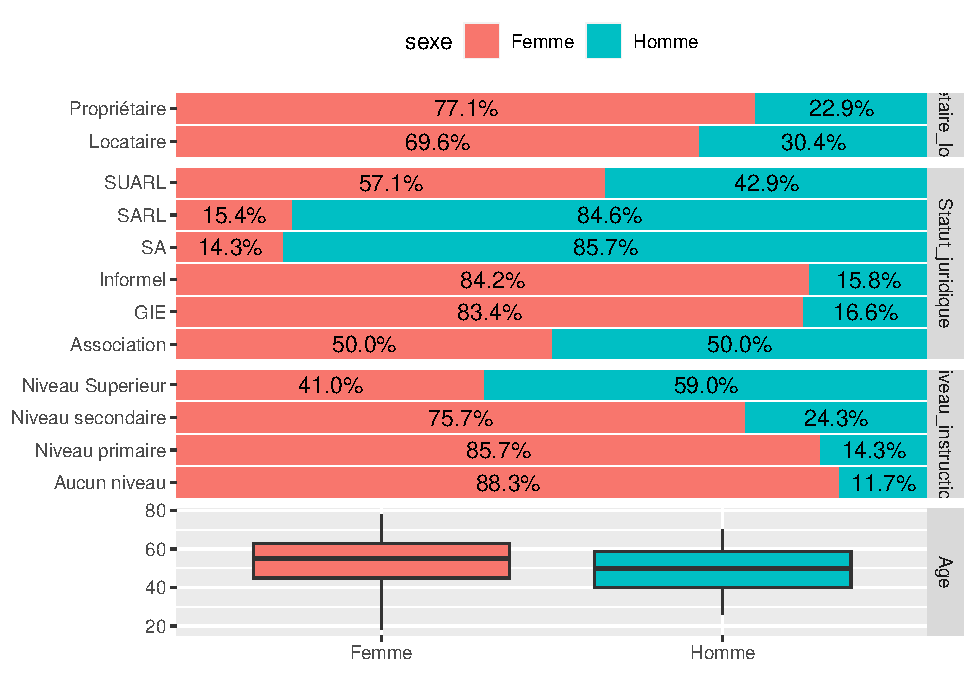
\includegraphics{Projet_R_ISE_1_files/figure-latex/unnamed-chunk-22-1} \end{center}

\hfill\break
ce graphique est une illustration plus synthétique des analyses
bivariées effectués

\textcolor{blue}{\subsubsection{Statistiques de choix.}}

\hypertarget{activituxe9-principale-de-lentreprise-par-filiuxe8re.}{%
\paragraph{Activité principale de l'entreprise par
filière.}\label{activituxe9-principale-de-lentreprise-par-filiuxe8re.}}

\hfill\break

\hypertarget{activite-principale-de-lentreprise-par-rapport-au-filiuxe8re}{%
\subparagraph{Activite principale de l'entreprise par rapport au
filière}\label{activite-principale-de-lentreprise-par-rapport-au-filiuxe8re}}

\hfill\break

\begin{Shaded}
\begin{Highlighting}[]
\CommentTok{\#}
\NormalTok{tab5}\OtherTok{=}\NormalTok{projet }\SpecialCharTok{\%\textgreater{}\%}
\NormalTok{    dplyr}\SpecialCharTok{::}\FunctionTok{select}\NormalTok{(q8, }\FunctionTok{starts\_with}\NormalTok{(}\StringTok{"filiere\_"}\NormalTok{)) }\SpecialCharTok{\%\textgreater{}\%}
  \FunctionTok{rename}\NormalTok{(}\StringTok{"Arachide"} \OtherTok{=}\NormalTok{ filiere\_1, }
             \StringTok{"Anacarde"}\OtherTok{=}\NormalTok{filiere\_2, }\StringTok{"Mangue"}\OtherTok{=}\NormalTok{ filiere\_3,}\StringTok{"Riz"}\OtherTok{=}\NormalTok{ filiere\_4) }\SpecialCharTok{\%\textgreater{}\%} 
      \FunctionTok{tbl\_summary}\NormalTok{(}\AttributeTok{by =}\NormalTok{ q8, }\AttributeTok{missing =} \StringTok{"no"}\NormalTok{)}\SpecialCharTok{\%\textgreater{}\%}
        \FunctionTok{modify\_spanning\_header}\NormalTok{(}\FunctionTok{everything}\NormalTok{() }\SpecialCharTok{\textasciitilde{}} \StringTok{"**Répartition des PME selon }
\StringTok{                               la filière et l\textquotesingle{}Activité }
\StringTok{                               principale de l’entreprise**"}\NormalTok{)}
\NormalTok{tab5}\SpecialCharTok{\%\textgreater{}\%} \FunctionTok{bold\_labels}\NormalTok{() }\SpecialCharTok{\%\textgreater{}\%} 
  \FunctionTok{italicize\_levels}\NormalTok{()  }\SpecialCharTok{\%\textgreater{}\%} 
  \FunctionTok{modify\_header}\NormalTok{(}\AttributeTok{update =} \FunctionTok{list}\NormalTok{( label }\SpecialCharTok{\textasciitilde{}} \StringTok{"**VARIABLE**"}\NormalTok{,}
                               \FunctionTok{all\_stat\_cols}\NormalTok{(}\AttributeTok{stat\_0 =} \ConstantTok{FALSE}\NormalTok{) }\SpecialCharTok{\textasciitilde{}} \StringTok{"**\{level\}**}
\StringTok{                               (n=\{n\},\{style\_percent(p)\}\%)"}
\NormalTok{  )) }\SpecialCharTok{\%\textgreater{}\%}  \FunctionTok{as\_flex\_table}\NormalTok{() }\SpecialCharTok{\%\textgreater{}\%}
  \FunctionTok{fontsize}\NormalTok{(}\AttributeTok{size =} \DecValTok{8}\NormalTok{) }\SpecialCharTok{\%\textgreater{}\%}
  \FunctionTok{width}\NormalTok{(}\AttributeTok{width =} \FloatTok{1.2}\NormalTok{)}
\end{Highlighting}
\end{Shaded}

\global\setlength{\Oldarrayrulewidth}{\arrayrulewidth}

\global\setlength{\Oldtabcolsep}{\tabcolsep}

\setlength{\tabcolsep}{0pt}

\renewcommand*{\arraystretch}{1.5}



\providecommand{\ascline}[3]{\noalign{\global\arrayrulewidth #1}\arrayrulecolor[HTML]{#2}\cline{#3}}

\begin{longtable}[c]{|p{1.20in}|p{1.20in}|p{1.20in}|p{1.20in}|p{1.20in}|p{1.20in}|p{1.20in}|p{1.20in}|p{1.20in}|p{1.20in}|p{1.20in}}



\ascline{1pt}{000000}{1-11}

\multicolumn{11}{>{\raggedright}m{\dimexpr 13.2in+20\tabcolsep}}{\textcolor[HTML]{000000}{\fontsize{11}{11}\selectfont{\textbf{**Répartition\ des\ PME\ selon\ }}}\textcolor[HTML]{000000}{\fontsize{11}{11}\selectfont{\textbf{\linebreak }}}\textcolor[HTML]{000000}{\fontsize{11}{11}\selectfont{\textbf{la\ filière\ et\ l'Activité\ }}}\textcolor[HTML]{000000}{\fontsize{11}{11}\selectfont{\textbf{\linebreak }}}\textcolor[HTML]{000000}{\fontsize{11}{11}\selectfont{\textbf{principale\ de\ l’entreprise**}}}} \\

\ascline{1pt}{000000}{1-11}



\multicolumn{1}{>{\raggedright}m{\dimexpr 1.2in+0\tabcolsep}}{\textcolor[HTML]{000000}{\fontsize{11}{11}\selectfont{\textbf{VARIABLE}}}} & \multicolumn{1}{>{\centering}m{\dimexpr 1.2in+0\tabcolsep}}{\textcolor[HTML]{000000}{\fontsize{11}{11}\selectfont{\textbf{Aucun}}}\textcolor[HTML]{000000}{\fontsize{11}{11}\selectfont{\linebreak }}\textcolor[HTML]{000000}{\fontsize{11}{11}\selectfont{(n=5,2.0\%)}}\textcolor[HTML]{000000}{\textsuperscript{\fontsize{11}{11}\selectfont{1}}}} & \multicolumn{1}{>{\centering}m{\dimexpr 1.2in+0\tabcolsep}}{\textcolor[HTML]{000000}{\fontsize{11}{11}\selectfont{\textbf{Autre\ a\ preciser}}}\textcolor[HTML]{000000}{\fontsize{11}{11}\selectfont{\linebreak }}\textcolor[HTML]{000000}{\fontsize{11}{11}\selectfont{(n=4,1.6\%)}}\textcolor[HTML]{000000}{\textsuperscript{\fontsize{11}{11}\selectfont{1}}}} & \multicolumn{1}{>{\centering}m{\dimexpr 1.2in+0\tabcolsep}}{\textcolor[HTML]{000000}{\fontsize{11}{11}\selectfont{\textbf{Tansformation\ d'autres\ céréales}}}\textcolor[HTML]{000000}{\fontsize{11}{11}\selectfont{\linebreak }}\textcolor[HTML]{000000}{\fontsize{11}{11}\selectfont{(n=57,23\%)}}\textcolor[HTML]{000000}{\textsuperscript{\fontsize{11}{11}\selectfont{1}}}} & \multicolumn{1}{>{\centering}m{\dimexpr 1.2in+0\tabcolsep}}{\textcolor[HTML]{000000}{\fontsize{11}{11}\selectfont{\textbf{Transformation\ d'autres\ fruits\ et\ legumes}}}\textcolor[HTML]{000000}{\fontsize{11}{11}\selectfont{\linebreak }}\textcolor[HTML]{000000}{\fontsize{11}{11}\selectfont{(n=14,5.6\%)}}\textcolor[HTML]{000000}{\textsuperscript{\fontsize{11}{11}\selectfont{1}}}} & \multicolumn{1}{>{\centering}m{\dimexpr 1.2in+0\tabcolsep}}{\textcolor[HTML]{000000}{\fontsize{11}{11}\selectfont{\textbf{Transformation\ d'autres\ produits\ oléagineux}}}\textcolor[HTML]{000000}{\fontsize{11}{11}\selectfont{\linebreak }}\textcolor[HTML]{000000}{\fontsize{11}{11}\selectfont{(n=1,0.4\%)}}\textcolor[HTML]{000000}{\textsuperscript{\fontsize{11}{11}\selectfont{1}}}} & \multicolumn{1}{>{\centering}m{\dimexpr 1.2in+0\tabcolsep}}{\textcolor[HTML]{000000}{\fontsize{11}{11}\selectfont{\textbf{Transformation\ de\ l'arachide}}}\textcolor[HTML]{000000}{\fontsize{11}{11}\selectfont{\linebreak }}\textcolor[HTML]{000000}{\fontsize{11}{11}\selectfont{(n=47,19\%)}}\textcolor[HTML]{000000}{\textsuperscript{\fontsize{11}{11}\selectfont{1}}}} & \multicolumn{1}{>{\centering}m{\dimexpr 1.2in+0\tabcolsep}}{\textcolor[HTML]{000000}{\fontsize{11}{11}\selectfont{\textbf{Transformation\ de\ la\ mangue}}}\textcolor[HTML]{000000}{\fontsize{11}{11}\selectfont{\linebreak }}\textcolor[HTML]{000000}{\fontsize{11}{11}\selectfont{(n=35,14\%)}}\textcolor[HTML]{000000}{\textsuperscript{\fontsize{11}{11}\selectfont{1}}}} & \multicolumn{1}{>{\centering}m{\dimexpr 1.2in+0\tabcolsep}}{\textcolor[HTML]{000000}{\fontsize{11}{11}\selectfont{\textbf{Transformation\ de\ la\ noix\ de\ cajoux}}}\textcolor[HTML]{000000}{\fontsize{11}{11}\selectfont{\linebreak }}\textcolor[HTML]{000000}{\fontsize{11}{11}\selectfont{(n=32,13\%)}}\textcolor[HTML]{000000}{\textsuperscript{\fontsize{11}{11}\selectfont{1}}}} & \multicolumn{1}{>{\centering}m{\dimexpr 1.2in+0\tabcolsep}}{\textcolor[HTML]{000000}{\fontsize{11}{11}\selectfont{\textbf{Transformation\ de\ la\ pomme\ de\ cajoux}}}\textcolor[HTML]{000000}{\fontsize{11}{11}\selectfont{\linebreak }}\textcolor[HTML]{000000}{\fontsize{11}{11}\selectfont{(n=9,3.6\%)}}\textcolor[HTML]{000000}{\textsuperscript{\fontsize{11}{11}\selectfont{1}}}} & \multicolumn{1}{>{\centering}m{\dimexpr 1.2in+0\tabcolsep}}{\textcolor[HTML]{000000}{\fontsize{11}{11}\selectfont{\textbf{Transformation\ du\ riz}}}\textcolor[HTML]{000000}{\fontsize{11}{11}\selectfont{\linebreak }}\textcolor[HTML]{000000}{\fontsize{11}{11}\selectfont{(n=46,18\%)}}\textcolor[HTML]{000000}{\textsuperscript{\fontsize{11}{11}\selectfont{1}}}} \\

\ascline{1pt}{000000}{1-11}\endfirsthead 

\ascline{1pt}{000000}{1-11}

\multicolumn{11}{>{\raggedright}m{\dimexpr 13.2in+20\tabcolsep}}{\textcolor[HTML]{000000}{\fontsize{11}{11}\selectfont{\textbf{**Répartition\ des\ PME\ selon\ }}}\textcolor[HTML]{000000}{\fontsize{11}{11}\selectfont{\textbf{\linebreak }}}\textcolor[HTML]{000000}{\fontsize{11}{11}\selectfont{\textbf{la\ filière\ et\ l'Activité\ }}}\textcolor[HTML]{000000}{\fontsize{11}{11}\selectfont{\textbf{\linebreak }}}\textcolor[HTML]{000000}{\fontsize{11}{11}\selectfont{\textbf{principale\ de\ l’entreprise**}}}} \\

\ascline{1pt}{000000}{1-11}



\multicolumn{1}{>{\raggedright}m{\dimexpr 1.2in+0\tabcolsep}}{\textcolor[HTML]{000000}{\fontsize{11}{11}\selectfont{\textbf{VARIABLE}}}} & \multicolumn{1}{>{\centering}m{\dimexpr 1.2in+0\tabcolsep}}{\textcolor[HTML]{000000}{\fontsize{11}{11}\selectfont{\textbf{Aucun}}}\textcolor[HTML]{000000}{\fontsize{11}{11}\selectfont{\linebreak }}\textcolor[HTML]{000000}{\fontsize{11}{11}\selectfont{(n=5,2.0\%)}}\textcolor[HTML]{000000}{\textsuperscript{\fontsize{11}{11}\selectfont{1}}}} & \multicolumn{1}{>{\centering}m{\dimexpr 1.2in+0\tabcolsep}}{\textcolor[HTML]{000000}{\fontsize{11}{11}\selectfont{\textbf{Autre\ a\ preciser}}}\textcolor[HTML]{000000}{\fontsize{11}{11}\selectfont{\linebreak }}\textcolor[HTML]{000000}{\fontsize{11}{11}\selectfont{(n=4,1.6\%)}}\textcolor[HTML]{000000}{\textsuperscript{\fontsize{11}{11}\selectfont{1}}}} & \multicolumn{1}{>{\centering}m{\dimexpr 1.2in+0\tabcolsep}}{\textcolor[HTML]{000000}{\fontsize{11}{11}\selectfont{\textbf{Tansformation\ d'autres\ céréales}}}\textcolor[HTML]{000000}{\fontsize{11}{11}\selectfont{\linebreak }}\textcolor[HTML]{000000}{\fontsize{11}{11}\selectfont{(n=57,23\%)}}\textcolor[HTML]{000000}{\textsuperscript{\fontsize{11}{11}\selectfont{1}}}} & \multicolumn{1}{>{\centering}m{\dimexpr 1.2in+0\tabcolsep}}{\textcolor[HTML]{000000}{\fontsize{11}{11}\selectfont{\textbf{Transformation\ d'autres\ fruits\ et\ legumes}}}\textcolor[HTML]{000000}{\fontsize{11}{11}\selectfont{\linebreak }}\textcolor[HTML]{000000}{\fontsize{11}{11}\selectfont{(n=14,5.6\%)}}\textcolor[HTML]{000000}{\textsuperscript{\fontsize{11}{11}\selectfont{1}}}} & \multicolumn{1}{>{\centering}m{\dimexpr 1.2in+0\tabcolsep}}{\textcolor[HTML]{000000}{\fontsize{11}{11}\selectfont{\textbf{Transformation\ d'autres\ produits\ oléagineux}}}\textcolor[HTML]{000000}{\fontsize{11}{11}\selectfont{\linebreak }}\textcolor[HTML]{000000}{\fontsize{11}{11}\selectfont{(n=1,0.4\%)}}\textcolor[HTML]{000000}{\textsuperscript{\fontsize{11}{11}\selectfont{1}}}} & \multicolumn{1}{>{\centering}m{\dimexpr 1.2in+0\tabcolsep}}{\textcolor[HTML]{000000}{\fontsize{11}{11}\selectfont{\textbf{Transformation\ de\ l'arachide}}}\textcolor[HTML]{000000}{\fontsize{11}{11}\selectfont{\linebreak }}\textcolor[HTML]{000000}{\fontsize{11}{11}\selectfont{(n=47,19\%)}}\textcolor[HTML]{000000}{\textsuperscript{\fontsize{11}{11}\selectfont{1}}}} & \multicolumn{1}{>{\centering}m{\dimexpr 1.2in+0\tabcolsep}}{\textcolor[HTML]{000000}{\fontsize{11}{11}\selectfont{\textbf{Transformation\ de\ la\ mangue}}}\textcolor[HTML]{000000}{\fontsize{11}{11}\selectfont{\linebreak }}\textcolor[HTML]{000000}{\fontsize{11}{11}\selectfont{(n=35,14\%)}}\textcolor[HTML]{000000}{\textsuperscript{\fontsize{11}{11}\selectfont{1}}}} & \multicolumn{1}{>{\centering}m{\dimexpr 1.2in+0\tabcolsep}}{\textcolor[HTML]{000000}{\fontsize{11}{11}\selectfont{\textbf{Transformation\ de\ la\ noix\ de\ cajoux}}}\textcolor[HTML]{000000}{\fontsize{11}{11}\selectfont{\linebreak }}\textcolor[HTML]{000000}{\fontsize{11}{11}\selectfont{(n=32,13\%)}}\textcolor[HTML]{000000}{\textsuperscript{\fontsize{11}{11}\selectfont{1}}}} & \multicolumn{1}{>{\centering}m{\dimexpr 1.2in+0\tabcolsep}}{\textcolor[HTML]{000000}{\fontsize{11}{11}\selectfont{\textbf{Transformation\ de\ la\ pomme\ de\ cajoux}}}\textcolor[HTML]{000000}{\fontsize{11}{11}\selectfont{\linebreak }}\textcolor[HTML]{000000}{\fontsize{11}{11}\selectfont{(n=9,3.6\%)}}\textcolor[HTML]{000000}{\textsuperscript{\fontsize{11}{11}\selectfont{1}}}} & \multicolumn{1}{>{\centering}m{\dimexpr 1.2in+0\tabcolsep}}{\textcolor[HTML]{000000}{\fontsize{11}{11}\selectfont{\textbf{Transformation\ du\ riz}}}\textcolor[HTML]{000000}{\fontsize{11}{11}\selectfont{\linebreak }}\textcolor[HTML]{000000}{\fontsize{11}{11}\selectfont{(n=46,18\%)}}\textcolor[HTML]{000000}{\textsuperscript{\fontsize{11}{11}\selectfont{1}}}} \\

\ascline{1pt}{000000}{1-11}\endhead



\multicolumn{11}{>{\raggedright}m{\dimexpr 13.2in+20\tabcolsep}}{\textcolor[HTML]{000000}{\textsuperscript{\fontsize{11}{11}\selectfont{1}}}\textcolor[HTML]{000000}{\fontsize{11}{11}\selectfont{n\ (\%)}}} \\

\endfoot



\multicolumn{1}{>{\raggedright}p{\dimexpr 1.2in+0\tabcolsep}}{\textcolor[HTML]{000000}{\fontsize{8}{8}\selectfont{\textbf{Arachide}}}} & \multicolumn{1}{>{\centering}p{\dimexpr 1.2in+0\tabcolsep}}{\textcolor[HTML]{000000}{\fontsize{8}{8}\selectfont{5\ (100\%)}}} & \multicolumn{1}{>{\centering}p{\dimexpr 1.2in+0\tabcolsep}}{\textcolor[HTML]{000000}{\fontsize{8}{8}\selectfont{1\ (25\%)}}} & \multicolumn{1}{>{\centering}p{\dimexpr 1.2in+0\tabcolsep}}{\textcolor[HTML]{000000}{\fontsize{8}{8}\selectfont{38\ (67\%)}}} & \multicolumn{1}{>{\centering}p{\dimexpr 1.2in+0\tabcolsep}}{\textcolor[HTML]{000000}{\fontsize{8}{8}\selectfont{7\ (50\%)}}} & \multicolumn{1}{>{\centering}p{\dimexpr 1.2in+0\tabcolsep}}{\textcolor[HTML]{000000}{\fontsize{8}{8}\selectfont{1\ (100\%)}}} & \multicolumn{1}{>{\centering}p{\dimexpr 1.2in+0\tabcolsep}}{\textcolor[HTML]{000000}{\fontsize{8}{8}\selectfont{47\ (100\%)}}} & \multicolumn{1}{>{\centering}p{\dimexpr 1.2in+0\tabcolsep}}{\textcolor[HTML]{000000}{\fontsize{8}{8}\selectfont{3\ (8.6\%)}}} & \multicolumn{1}{>{\centering}p{\dimexpr 1.2in+0\tabcolsep}}{\textcolor[HTML]{000000}{\fontsize{8}{8}\selectfont{3\ (9.4\%)}}} & \multicolumn{1}{>{\centering}p{\dimexpr 1.2in+0\tabcolsep}}{\textcolor[HTML]{000000}{\fontsize{8}{8}\selectfont{1\ (11\%)}}} & \multicolumn{1}{>{\centering}p{\dimexpr 1.2in+0\tabcolsep}}{\textcolor[HTML]{000000}{\fontsize{8}{8}\selectfont{2\ (4.3\%)}}} \\





\multicolumn{1}{>{\raggedright}p{\dimexpr 1.2in+0\tabcolsep}}{\textcolor[HTML]{000000}{\fontsize{8}{8}\selectfont{\textbf{Anacarde}}}} & \multicolumn{1}{>{\centering}p{\dimexpr 1.2in+0\tabcolsep}}{\textcolor[HTML]{000000}{\fontsize{8}{8}\selectfont{0\ (0\%)}}} & \multicolumn{1}{>{\centering}p{\dimexpr 1.2in+0\tabcolsep}}{\textcolor[HTML]{000000}{\fontsize{8}{8}\selectfont{0\ (0\%)}}} & \multicolumn{1}{>{\centering}p{\dimexpr 1.2in+0\tabcolsep}}{\textcolor[HTML]{000000}{\fontsize{8}{8}\selectfont{1\ (1.8\%)}}} & \multicolumn{1}{>{\centering}p{\dimexpr 1.2in+0\tabcolsep}}{\textcolor[HTML]{000000}{\fontsize{8}{8}\selectfont{2\ (14\%)}}} & \multicolumn{1}{>{\centering}p{\dimexpr 1.2in+0\tabcolsep}}{\textcolor[HTML]{000000}{\fontsize{8}{8}\selectfont{0\ (0\%)}}} & \multicolumn{1}{>{\centering}p{\dimexpr 1.2in+0\tabcolsep}}{\textcolor[HTML]{000000}{\fontsize{8}{8}\selectfont{4\ (8.5\%)}}} & \multicolumn{1}{>{\centering}p{\dimexpr 1.2in+0\tabcolsep}}{\textcolor[HTML]{000000}{\fontsize{8}{8}\selectfont{13\ (37\%)}}} & \multicolumn{1}{>{\centering}p{\dimexpr 1.2in+0\tabcolsep}}{\textcolor[HTML]{000000}{\fontsize{8}{8}\selectfont{32\ (100\%)}}} & \multicolumn{1}{>{\centering}p{\dimexpr 1.2in+0\tabcolsep}}{\textcolor[HTML]{000000}{\fontsize{8}{8}\selectfont{9\ (100\%)}}} & \multicolumn{1}{>{\centering}p{\dimexpr 1.2in+0\tabcolsep}}{\textcolor[HTML]{000000}{\fontsize{8}{8}\selectfont{0\ (0\%)}}} \\





\multicolumn{1}{>{\raggedright}p{\dimexpr 1.2in+0\tabcolsep}}{\textcolor[HTML]{000000}{\fontsize{8}{8}\selectfont{\textbf{Mangue}}}} & \multicolumn{1}{>{\centering}p{\dimexpr 1.2in+0\tabcolsep}}{\textcolor[HTML]{000000}{\fontsize{8}{8}\selectfont{0\ (0\%)}}} & \multicolumn{1}{>{\centering}p{\dimexpr 1.2in+0\tabcolsep}}{\textcolor[HTML]{000000}{\fontsize{8}{8}\selectfont{0\ (0\%)}}} & \multicolumn{1}{>{\centering}p{\dimexpr 1.2in+0\tabcolsep}}{\textcolor[HTML]{000000}{\fontsize{8}{8}\selectfont{28\ (49\%)}}} & \multicolumn{1}{>{\centering}p{\dimexpr 1.2in+0\tabcolsep}}{\textcolor[HTML]{000000}{\fontsize{8}{8}\selectfont{6\ (43\%)}}} & \multicolumn{1}{>{\centering}p{\dimexpr 1.2in+0\tabcolsep}}{\textcolor[HTML]{000000}{\fontsize{8}{8}\selectfont{0\ (0\%)}}} & \multicolumn{1}{>{\centering}p{\dimexpr 1.2in+0\tabcolsep}}{\textcolor[HTML]{000000}{\fontsize{8}{8}\selectfont{4\ (8.5\%)}}} & \multicolumn{1}{>{\centering}p{\dimexpr 1.2in+0\tabcolsep}}{\textcolor[HTML]{000000}{\fontsize{8}{8}\selectfont{2\ (5.7\%)}}} & \multicolumn{1}{>{\centering}p{\dimexpr 1.2in+0\tabcolsep}}{\textcolor[HTML]{000000}{\fontsize{8}{8}\selectfont{0\ (0\%)}}} & \multicolumn{1}{>{\centering}p{\dimexpr 1.2in+0\tabcolsep}}{\textcolor[HTML]{000000}{\fontsize{8}{8}\selectfont{3\ (33\%)}}} & \multicolumn{1}{>{\centering}p{\dimexpr 1.2in+0\tabcolsep}}{\textcolor[HTML]{000000}{\fontsize{8}{8}\selectfont{46\ (100\%)}}} \\





\multicolumn{1}{>{\raggedright}p{\dimexpr 1.2in+0\tabcolsep}}{\textcolor[HTML]{000000}{\fontsize{8}{8}\selectfont{\textbf{Riz}}}} & \multicolumn{1}{>{\centering}p{\dimexpr 1.2in+0\tabcolsep}}{\textcolor[HTML]{000000}{\fontsize{8}{8}\selectfont{0\ (0\%)}}} & \multicolumn{1}{>{\centering}p{\dimexpr 1.2in+0\tabcolsep}}{\textcolor[HTML]{000000}{\fontsize{8}{8}\selectfont{3\ (75\%)}}} & \multicolumn{1}{>{\centering}p{\dimexpr 1.2in+0\tabcolsep}}{\textcolor[HTML]{000000}{\fontsize{8}{8}\selectfont{21\ (37\%)}}} & \multicolumn{1}{>{\centering}p{\dimexpr 1.2in+0\tabcolsep}}{\textcolor[HTML]{000000}{\fontsize{8}{8}\selectfont{9\ (64\%)}}} & \multicolumn{1}{>{\centering}p{\dimexpr 1.2in+0\tabcolsep}}{\textcolor[HTML]{000000}{\fontsize{8}{8}\selectfont{0\ (0\%)}}} & \multicolumn{1}{>{\centering}p{\dimexpr 1.2in+0\tabcolsep}}{\textcolor[HTML]{000000}{\fontsize{8}{8}\selectfont{4\ (8.5\%)}}} & \multicolumn{1}{>{\centering}p{\dimexpr 1.2in+0\tabcolsep}}{\textcolor[HTML]{000000}{\fontsize{8}{8}\selectfont{35\ (100\%)}}} & \multicolumn{1}{>{\centering}p{\dimexpr 1.2in+0\tabcolsep}}{\textcolor[HTML]{000000}{\fontsize{8}{8}\selectfont{7\ (22\%)}}} & \multicolumn{1}{>{\centering}p{\dimexpr 1.2in+0\tabcolsep}}{\textcolor[HTML]{000000}{\fontsize{8}{8}\selectfont{9\ (100\%)}}} & \multicolumn{1}{>{\centering}p{\dimexpr 1.2in+0\tabcolsep}}{\textcolor[HTML]{000000}{\fontsize{8}{8}\selectfont{4\ (8.7\%)}}} \\

\ascline{1pt}{000000}{1-11}



\end{longtable}



\arrayrulecolor[HTML]{000000}

\global\setlength{\arrayrulewidth}{\Oldarrayrulewidth}

\global\setlength{\tabcolsep}{\Oldtabcolsep}

\renewcommand*{\arraystretch}{1}

\hfill\break

L'analyse des croisements entre filières et activités principales des
PME met en évidence des informations intéressantes. Parmi les
différentes filières, la transformation de l'arachide et du riz se
distingue comme les activités principales les plus fréquentes,
représentant respectivement 19\% et 18\% des PME étudiées. Dans la
filière de l'arachide, toutes les PME sont engagées dans cette activité,
et une grande majorité (67\%) sont exclusivement dédiées à cette
transformation. Dans la filière du riz, une proportion significative
(37\%) se concentre uniquement sur cette transformation. La
transformation d'autres céréales et de fruits et légumes est également
représentée, avec des pourcentages de 23\% et 5,6\% respectivement. La
transformation de la mangue est principalement présente dans la filière
de l'anacarde (49\%) et du riz (43\%).

\hfill\break

\hypertarget{activituxe9-principale-suivant-les-spuxe9cificituxe9s-des-filiuxe8res}{%
\subparagraph{Activité principale suivant les spécificités des
filières}\label{activituxe9-principale-suivant-les-spuxe9cificituxe9s-des-filiuxe8res}}

\hfill\break

\begin{Shaded}
\begin{Highlighting}[]
\CommentTok{\#plus spécifiquement}
\NormalTok{tab6}\OtherTok{=}\NormalTok{projet }\SpecialCharTok{\%\textgreater{}\%}
\NormalTok{  dplyr}\SpecialCharTok{::}\FunctionTok{select}\NormalTok{(q8, nom\_filiere) }\SpecialCharTok{\%\textgreater{}\%}
     \FunctionTok{rename}\NormalTok{(}\StringTok{"Activité principale"}\OtherTok{=}\NormalTok{q8) }\SpecialCharTok{\%\textgreater{}\%} 
       \FunctionTok{tbl\_summary}\NormalTok{(}\AttributeTok{by =}\NormalTok{ nom\_filiere, }\AttributeTok{missing =} \StringTok{"no"}\NormalTok{)}\SpecialCharTok{\%\textgreater{}\%}
       \FunctionTok{modify\_spanning\_header}\NormalTok{(}\FunctionTok{everything}\NormalTok{() }\SpecialCharTok{\textasciitilde{}} 
                                \StringTok{"**Répartition des PME selon }
\StringTok{                              la filière et l\textquotesingle{}Activité principale }
\StringTok{                              de l’entreprise**"}\NormalTok{) }
\NormalTok{tab6}\SpecialCharTok{\%\textgreater{}\%} \FunctionTok{bold\_labels}\NormalTok{() }\SpecialCharTok{\%\textgreater{}\%} 
  \FunctionTok{italicize\_levels}\NormalTok{()  }\SpecialCharTok{\%\textgreater{}\%} 
  \FunctionTok{modify\_header}\NormalTok{(}\AttributeTok{update =} \FunctionTok{list}\NormalTok{( label }\SpecialCharTok{\textasciitilde{}} \StringTok{"**VARIABLE**"}\NormalTok{, }
                               \FunctionTok{all\_stat\_cols}\NormalTok{(}\AttributeTok{stat\_0 =} \ConstantTok{FALSE}\NormalTok{) }\SpecialCharTok{\textasciitilde{}} 
                                 \StringTok{"**\{level\}** (n=\{n\}, \{style\_percent(p)\}\%)"}
\NormalTok{  )) }\SpecialCharTok{\%\textgreater{}\%}  \FunctionTok{as\_flex\_table}\NormalTok{() }\SpecialCharTok{\%\textgreater{}\%}
  \FunctionTok{fontsize}\NormalTok{(}\AttributeTok{size =} \DecValTok{8}\NormalTok{) }\SpecialCharTok{\%\textgreater{}\%}
  \FunctionTok{width}\NormalTok{(}\AttributeTok{width =} \FloatTok{1.1}\NormalTok{)}
\end{Highlighting}
\end{Shaded}

\global\setlength{\Oldarrayrulewidth}{\arrayrulewidth}

\global\setlength{\Oldtabcolsep}{\tabcolsep}

\setlength{\tabcolsep}{0pt}

\renewcommand*{\arraystretch}{1.5}



\providecommand{\ascline}[3]{\noalign{\global\arrayrulewidth #1}\arrayrulecolor[HTML]{#2}\cline{#3}}

\begin{longtable}[c]{|p{1.10in}|p{1.10in}|p{1.10in}|p{1.10in}|p{1.10in}|p{1.10in}|p{1.10in}|p{1.10in}|p{1.10in}|p{1.10in}|p{1.10in}|p{1.10in}|p{1.10in}|p{1.10in}|p{1.10in}}



\ascline{1pt}{000000}{1-15}

\multicolumn{15}{>{\raggedright}m{\dimexpr 16.5in+28\tabcolsep}}{\textcolor[HTML]{000000}{\fontsize{11}{11}\selectfont{\textbf{**Répartition\ des\ PME\ selon\ }}}\textcolor[HTML]{000000}{\fontsize{11}{11}\selectfont{\textbf{\linebreak }}}\textcolor[HTML]{000000}{\fontsize{11}{11}\selectfont{\textbf{la\ filière\ et\ l'Activité\ principale\ }}}\textcolor[HTML]{000000}{\fontsize{11}{11}\selectfont{\textbf{\linebreak }}}\textcolor[HTML]{000000}{\fontsize{11}{11}\selectfont{\textbf{de\ l’entreprise**}}}} \\

\ascline{1pt}{000000}{1-15}



\multicolumn{1}{>{\raggedright}m{\dimexpr 1.1in+0\tabcolsep}}{\textcolor[HTML]{000000}{\fontsize{11}{11}\selectfont{\textbf{VARIABLE}}}} & \multicolumn{1}{>{\centering}m{\dimexpr 1.1in+0\tabcolsep}}{\textcolor[HTML]{000000}{\fontsize{11}{11}\selectfont{\textbf{anacarde}}}\textcolor[HTML]{000000}{\fontsize{11}{11}\selectfont{\ (n=25,\ 10\%)}}\textcolor[HTML]{000000}{\textsuperscript{\fontsize{11}{11}\selectfont{1}}}} & \multicolumn{1}{>{\centering}m{\dimexpr 1.1in+0\tabcolsep}}{\textcolor[HTML]{000000}{\fontsize{11}{11}\selectfont{\textbf{arachide}}}\textcolor[HTML]{000000}{\fontsize{11}{11}\selectfont{\ (n=61,\ 24\%)}}\textcolor[HTML]{000000}{\textsuperscript{\fontsize{11}{11}\selectfont{1}}}} & \multicolumn{1}{>{\centering}m{\dimexpr 1.1in+0\tabcolsep}}{\textcolor[HTML]{000000}{\fontsize{11}{11}\selectfont{**arachide\ }}\textcolor[HTML]{000000}{\fontsize{11}{11}\selectfont{\linebreak }}\textcolor[HTML]{000000}{\fontsize{11}{11}\selectfont{\ \ \ \ \ \ \ \ \ \ \ \ \&\ anacarde\ \&\ mangue\&\ riz**\ (n=1,\ 0.4\%)}}\textcolor[HTML]{000000}{\textsuperscript{\fontsize{11}{11}\selectfont{1}}}} & \multicolumn{1}{>{\centering}m{\dimexpr 1.1in+0\tabcolsep}}{\textcolor[HTML]{000000}{\fontsize{11}{11}\selectfont{**arachide\ \&\ }}\textcolor[HTML]{000000}{\fontsize{11}{11}\selectfont{\linebreak }}\textcolor[HTML]{000000}{\fontsize{11}{11}\selectfont{\ \ \ \ \ \ \ \ \ \ \ \ anacarde\ \&\ mangue**\ (n=1,\ 0.4\%)}}\textcolor[HTML]{000000}{\textsuperscript{\fontsize{11}{11}\selectfont{1}}}} & \multicolumn{1}{>{\centering}m{\dimexpr 1.1in+0\tabcolsep}}{\textcolor[HTML]{000000}{\fontsize{11}{11}\selectfont{\textbf{arachide\ \&\ anacarde}}}\textcolor[HTML]{000000}{\fontsize{11}{11}\selectfont{\ (n=6,\ 2.4\%)}}\textcolor[HTML]{000000}{\textsuperscript{\fontsize{11}{11}\selectfont{1}}}} & \multicolumn{1}{>{\centering}m{\dimexpr 1.1in+0\tabcolsep}}{\textcolor[HTML]{000000}{\fontsize{11}{11}\selectfont{\textbf{arachide\ \&\ anacarde\ \&\ riz}}}\textcolor[HTML]{000000}{\fontsize{11}{11}\selectfont{\ (n=2,\ 0.8\%)}}\textcolor[HTML]{000000}{\textsuperscript{\fontsize{11}{11}\selectfont{1}}}} & \multicolumn{1}{>{\centering}m{\dimexpr 1.1in+0\tabcolsep}}{\textcolor[HTML]{000000}{\fontsize{11}{11}\selectfont{\textbf{arachide\ \&\ mangue}}}\textcolor[HTML]{000000}{\fontsize{11}{11}\selectfont{\ (n=13,\ 5.2\%)}}\textcolor[HTML]{000000}{\textsuperscript{\fontsize{11}{11}\selectfont{1}}}} & \multicolumn{1}{>{\centering}m{\dimexpr 1.1in+0\tabcolsep}}{\textcolor[HTML]{000000}{\fontsize{11}{11}\selectfont{\textbf{arachide\ \&\ riz}}}\textcolor[HTML]{000000}{\fontsize{11}{11}\selectfont{\ (n=11,\ 4.4\%)}}\textcolor[HTML]{000000}{\textsuperscript{\fontsize{11}{11}\selectfont{1}}}} & \multicolumn{1}{>{\centering}m{\dimexpr 1.1in+0\tabcolsep}}{\textcolor[HTML]{000000}{\fontsize{11}{11}\selectfont{\textbf{arachide\ \&\ riz\ \&\ mangue}}}\textcolor[HTML]{000000}{\fontsize{11}{11}\selectfont{\ (n=13,\ 5.2\%)}}\textcolor[HTML]{000000}{\textsuperscript{\fontsize{11}{11}\selectfont{1}}}} & \multicolumn{1}{>{\centering}m{\dimexpr 1.1in+0\tabcolsep}}{\textcolor[HTML]{000000}{\fontsize{11}{11}\selectfont{\textbf{mangue}}}\textcolor[HTML]{000000}{\fontsize{11}{11}\selectfont{\ (n=52,\ 21\%)}}\textcolor[HTML]{000000}{\textsuperscript{\fontsize{11}{11}\selectfont{1}}}} & \multicolumn{1}{>{\centering}m{\dimexpr 1.1in+0\tabcolsep}}{\textcolor[HTML]{000000}{\fontsize{11}{11}\selectfont{\textbf{riz}}}\textcolor[HTML]{000000}{\fontsize{11}{11}\selectfont{\ (n=33,\ 13\%)}}\textcolor[HTML]{000000}{\textsuperscript{\fontsize{11}{11}\selectfont{1}}}} & \multicolumn{1}{>{\centering}m{\dimexpr 1.1in+0\tabcolsep}}{\textcolor[HTML]{000000}{\fontsize{11}{11}\selectfont{\textbf{riz\ \&\ anacarde}}}\textcolor[HTML]{000000}{\fontsize{11}{11}\selectfont{\ (n=23,\ 9.2\%)}}\textcolor[HTML]{000000}{\textsuperscript{\fontsize{11}{11}\selectfont{1}}}} & \multicolumn{1}{>{\centering}m{\dimexpr 1.1in+0\tabcolsep}}{\textcolor[HTML]{000000}{\fontsize{11}{11}\selectfont{\textbf{riz\ \&\ anacarde\ \&\ mangue}}}\textcolor[HTML]{000000}{\fontsize{11}{11}\selectfont{\ (n=3,\ 1.2\%)}}\textcolor[HTML]{000000}{\textsuperscript{\fontsize{11}{11}\selectfont{1}}}} & \multicolumn{1}{>{\centering}m{\dimexpr 1.1in+0\tabcolsep}}{\textcolor[HTML]{000000}{\fontsize{11}{11}\selectfont{\textbf{riz\ \&\ mangue}}}\textcolor[HTML]{000000}{\fontsize{11}{11}\selectfont{\ (n=6,\ 2.4\%)}}\textcolor[HTML]{000000}{\textsuperscript{\fontsize{11}{11}\selectfont{1}}}} \\

\ascline{1pt}{000000}{1-15}\endfirsthead 

\ascline{1pt}{000000}{1-15}

\multicolumn{15}{>{\raggedright}m{\dimexpr 16.5in+28\tabcolsep}}{\textcolor[HTML]{000000}{\fontsize{11}{11}\selectfont{\textbf{**Répartition\ des\ PME\ selon\ }}}\textcolor[HTML]{000000}{\fontsize{11}{11}\selectfont{\textbf{\linebreak }}}\textcolor[HTML]{000000}{\fontsize{11}{11}\selectfont{\textbf{la\ filière\ et\ l'Activité\ principale\ }}}\textcolor[HTML]{000000}{\fontsize{11}{11}\selectfont{\textbf{\linebreak }}}\textcolor[HTML]{000000}{\fontsize{11}{11}\selectfont{\textbf{de\ l’entreprise**}}}} \\

\ascline{1pt}{000000}{1-15}



\multicolumn{1}{>{\raggedright}m{\dimexpr 1.1in+0\tabcolsep}}{\textcolor[HTML]{000000}{\fontsize{11}{11}\selectfont{\textbf{VARIABLE}}}} & \multicolumn{1}{>{\centering}m{\dimexpr 1.1in+0\tabcolsep}}{\textcolor[HTML]{000000}{\fontsize{11}{11}\selectfont{\textbf{anacarde}}}\textcolor[HTML]{000000}{\fontsize{11}{11}\selectfont{\ (n=25,\ 10\%)}}\textcolor[HTML]{000000}{\textsuperscript{\fontsize{11}{11}\selectfont{1}}}} & \multicolumn{1}{>{\centering}m{\dimexpr 1.1in+0\tabcolsep}}{\textcolor[HTML]{000000}{\fontsize{11}{11}\selectfont{\textbf{arachide}}}\textcolor[HTML]{000000}{\fontsize{11}{11}\selectfont{\ (n=61,\ 24\%)}}\textcolor[HTML]{000000}{\textsuperscript{\fontsize{11}{11}\selectfont{1}}}} & \multicolumn{1}{>{\centering}m{\dimexpr 1.1in+0\tabcolsep}}{\textcolor[HTML]{000000}{\fontsize{11}{11}\selectfont{**arachide\ }}\textcolor[HTML]{000000}{\fontsize{11}{11}\selectfont{\linebreak }}\textcolor[HTML]{000000}{\fontsize{11}{11}\selectfont{\ \ \ \ \ \ \ \ \ \ \ \ \&\ anacarde\ \&\ mangue\&\ riz**\ (n=1,\ 0.4\%)}}\textcolor[HTML]{000000}{\textsuperscript{\fontsize{11}{11}\selectfont{1}}}} & \multicolumn{1}{>{\centering}m{\dimexpr 1.1in+0\tabcolsep}}{\textcolor[HTML]{000000}{\fontsize{11}{11}\selectfont{**arachide\ \&\ }}\textcolor[HTML]{000000}{\fontsize{11}{11}\selectfont{\linebreak }}\textcolor[HTML]{000000}{\fontsize{11}{11}\selectfont{\ \ \ \ \ \ \ \ \ \ \ \ anacarde\ \&\ mangue**\ (n=1,\ 0.4\%)}}\textcolor[HTML]{000000}{\textsuperscript{\fontsize{11}{11}\selectfont{1}}}} & \multicolumn{1}{>{\centering}m{\dimexpr 1.1in+0\tabcolsep}}{\textcolor[HTML]{000000}{\fontsize{11}{11}\selectfont{\textbf{arachide\ \&\ anacarde}}}\textcolor[HTML]{000000}{\fontsize{11}{11}\selectfont{\ (n=6,\ 2.4\%)}}\textcolor[HTML]{000000}{\textsuperscript{\fontsize{11}{11}\selectfont{1}}}} & \multicolumn{1}{>{\centering}m{\dimexpr 1.1in+0\tabcolsep}}{\textcolor[HTML]{000000}{\fontsize{11}{11}\selectfont{\textbf{arachide\ \&\ anacarde\ \&\ riz}}}\textcolor[HTML]{000000}{\fontsize{11}{11}\selectfont{\ (n=2,\ 0.8\%)}}\textcolor[HTML]{000000}{\textsuperscript{\fontsize{11}{11}\selectfont{1}}}} & \multicolumn{1}{>{\centering}m{\dimexpr 1.1in+0\tabcolsep}}{\textcolor[HTML]{000000}{\fontsize{11}{11}\selectfont{\textbf{arachide\ \&\ mangue}}}\textcolor[HTML]{000000}{\fontsize{11}{11}\selectfont{\ (n=13,\ 5.2\%)}}\textcolor[HTML]{000000}{\textsuperscript{\fontsize{11}{11}\selectfont{1}}}} & \multicolumn{1}{>{\centering}m{\dimexpr 1.1in+0\tabcolsep}}{\textcolor[HTML]{000000}{\fontsize{11}{11}\selectfont{\textbf{arachide\ \&\ riz}}}\textcolor[HTML]{000000}{\fontsize{11}{11}\selectfont{\ (n=11,\ 4.4\%)}}\textcolor[HTML]{000000}{\textsuperscript{\fontsize{11}{11}\selectfont{1}}}} & \multicolumn{1}{>{\centering}m{\dimexpr 1.1in+0\tabcolsep}}{\textcolor[HTML]{000000}{\fontsize{11}{11}\selectfont{\textbf{arachide\ \&\ riz\ \&\ mangue}}}\textcolor[HTML]{000000}{\fontsize{11}{11}\selectfont{\ (n=13,\ 5.2\%)}}\textcolor[HTML]{000000}{\textsuperscript{\fontsize{11}{11}\selectfont{1}}}} & \multicolumn{1}{>{\centering}m{\dimexpr 1.1in+0\tabcolsep}}{\textcolor[HTML]{000000}{\fontsize{11}{11}\selectfont{\textbf{mangue}}}\textcolor[HTML]{000000}{\fontsize{11}{11}\selectfont{\ (n=52,\ 21\%)}}\textcolor[HTML]{000000}{\textsuperscript{\fontsize{11}{11}\selectfont{1}}}} & \multicolumn{1}{>{\centering}m{\dimexpr 1.1in+0\tabcolsep}}{\textcolor[HTML]{000000}{\fontsize{11}{11}\selectfont{\textbf{riz}}}\textcolor[HTML]{000000}{\fontsize{11}{11}\selectfont{\ (n=33,\ 13\%)}}\textcolor[HTML]{000000}{\textsuperscript{\fontsize{11}{11}\selectfont{1}}}} & \multicolumn{1}{>{\centering}m{\dimexpr 1.1in+0\tabcolsep}}{\textcolor[HTML]{000000}{\fontsize{11}{11}\selectfont{\textbf{riz\ \&\ anacarde}}}\textcolor[HTML]{000000}{\fontsize{11}{11}\selectfont{\ (n=23,\ 9.2\%)}}\textcolor[HTML]{000000}{\textsuperscript{\fontsize{11}{11}\selectfont{1}}}} & \multicolumn{1}{>{\centering}m{\dimexpr 1.1in+0\tabcolsep}}{\textcolor[HTML]{000000}{\fontsize{11}{11}\selectfont{\textbf{riz\ \&\ anacarde\ \&\ mangue}}}\textcolor[HTML]{000000}{\fontsize{11}{11}\selectfont{\ (n=3,\ 1.2\%)}}\textcolor[HTML]{000000}{\textsuperscript{\fontsize{11}{11}\selectfont{1}}}} & \multicolumn{1}{>{\centering}m{\dimexpr 1.1in+0\tabcolsep}}{\textcolor[HTML]{000000}{\fontsize{11}{11}\selectfont{\textbf{riz\ \&\ mangue}}}\textcolor[HTML]{000000}{\fontsize{11}{11}\selectfont{\ (n=6,\ 2.4\%)}}\textcolor[HTML]{000000}{\textsuperscript{\fontsize{11}{11}\selectfont{1}}}} \\

\ascline{1pt}{000000}{1-15}\endhead



\multicolumn{15}{>{\raggedright}m{\dimexpr 16.5in+28\tabcolsep}}{\textcolor[HTML]{000000}{\textsuperscript{\fontsize{11}{11}\selectfont{1}}}\textcolor[HTML]{000000}{\fontsize{11}{11}\selectfont{n\ (\%)}}} \\

\endfoot



\multicolumn{1}{>{\raggedright}p{\dimexpr 1.1in+0\tabcolsep}}{\textcolor[HTML]{000000}{\fontsize{8}{8}\selectfont{\textbf{Activité\ principale}}}} & \multicolumn{1}{>{\centering}p{\dimexpr 1.1in+0\tabcolsep}}{\textcolor[HTML]{000000}{\fontsize{8}{8}\selectfont{}}} & \multicolumn{1}{>{\centering}p{\dimexpr 1.1in+0\tabcolsep}}{\textcolor[HTML]{000000}{\fontsize{8}{8}\selectfont{}}} & \multicolumn{1}{>{\centering}p{\dimexpr 1.1in+0\tabcolsep}}{\textcolor[HTML]{000000}{\fontsize{8}{8}\selectfont{}}} & \multicolumn{1}{>{\centering}p{\dimexpr 1.1in+0\tabcolsep}}{\textcolor[HTML]{000000}{\fontsize{8}{8}\selectfont{}}} & \multicolumn{1}{>{\centering}p{\dimexpr 1.1in+0\tabcolsep}}{\textcolor[HTML]{000000}{\fontsize{8}{8}\selectfont{}}} & \multicolumn{1}{>{\centering}p{\dimexpr 1.1in+0\tabcolsep}}{\textcolor[HTML]{000000}{\fontsize{8}{8}\selectfont{}}} & \multicolumn{1}{>{\centering}p{\dimexpr 1.1in+0\tabcolsep}}{\textcolor[HTML]{000000}{\fontsize{8}{8}\selectfont{}}} & \multicolumn{1}{>{\centering}p{\dimexpr 1.1in+0\tabcolsep}}{\textcolor[HTML]{000000}{\fontsize{8}{8}\selectfont{}}} & \multicolumn{1}{>{\centering}p{\dimexpr 1.1in+0\tabcolsep}}{\textcolor[HTML]{000000}{\fontsize{8}{8}\selectfont{}}} & \multicolumn{1}{>{\centering}p{\dimexpr 1.1in+0\tabcolsep}}{\textcolor[HTML]{000000}{\fontsize{8}{8}\selectfont{}}} & \multicolumn{1}{>{\centering}p{\dimexpr 1.1in+0\tabcolsep}}{\textcolor[HTML]{000000}{\fontsize{8}{8}\selectfont{}}} & \multicolumn{1}{>{\centering}p{\dimexpr 1.1in+0\tabcolsep}}{\textcolor[HTML]{000000}{\fontsize{8}{8}\selectfont{}}} & \multicolumn{1}{>{\centering}p{\dimexpr 1.1in+0\tabcolsep}}{\textcolor[HTML]{000000}{\fontsize{8}{8}\selectfont{}}} & \multicolumn{1}{>{\centering}p{\dimexpr 1.1in+0\tabcolsep}}{\textcolor[HTML]{000000}{\fontsize{8}{8}\selectfont{}}} \\





\multicolumn{1}{>{\raggedright}p{\dimexpr 1.1in+0\tabcolsep}}{\textcolor[HTML]{000000}{\fontsize{8}{8}\selectfont{\textit{Aucun}}}} & \multicolumn{1}{>{\centering}p{\dimexpr 1.1in+0\tabcolsep}}{\textcolor[HTML]{000000}{\fontsize{8}{8}\selectfont{0\ (0\%)}}} & \multicolumn{1}{>{\centering}p{\dimexpr 1.1in+0\tabcolsep}}{\textcolor[HTML]{000000}{\fontsize{8}{8}\selectfont{5\ (8.2\%)}}} & \multicolumn{1}{>{\centering}p{\dimexpr 1.1in+0\tabcolsep}}{\textcolor[HTML]{000000}{\fontsize{8}{8}\selectfont{0\ (0\%)}}} & \multicolumn{1}{>{\centering}p{\dimexpr 1.1in+0\tabcolsep}}{\textcolor[HTML]{000000}{\fontsize{8}{8}\selectfont{0\ (0\%)}}} & \multicolumn{1}{>{\centering}p{\dimexpr 1.1in+0\tabcolsep}}{\textcolor[HTML]{000000}{\fontsize{8}{8}\selectfont{0\ (0\%)}}} & \multicolumn{1}{>{\centering}p{\dimexpr 1.1in+0\tabcolsep}}{\textcolor[HTML]{000000}{\fontsize{8}{8}\selectfont{0\ (0\%)}}} & \multicolumn{1}{>{\centering}p{\dimexpr 1.1in+0\tabcolsep}}{\textcolor[HTML]{000000}{\fontsize{8}{8}\selectfont{0\ (0\%)}}} & \multicolumn{1}{>{\centering}p{\dimexpr 1.1in+0\tabcolsep}}{\textcolor[HTML]{000000}{\fontsize{8}{8}\selectfont{0\ (0\%)}}} & \multicolumn{1}{>{\centering}p{\dimexpr 1.1in+0\tabcolsep}}{\textcolor[HTML]{000000}{\fontsize{8}{8}\selectfont{0\ (0\%)}}} & \multicolumn{1}{>{\centering}p{\dimexpr 1.1in+0\tabcolsep}}{\textcolor[HTML]{000000}{\fontsize{8}{8}\selectfont{0\ (0\%)}}} & \multicolumn{1}{>{\centering}p{\dimexpr 1.1in+0\tabcolsep}}{\textcolor[HTML]{000000}{\fontsize{8}{8}\selectfont{0\ (0\%)}}} & \multicolumn{1}{>{\centering}p{\dimexpr 1.1in+0\tabcolsep}}{\textcolor[HTML]{000000}{\fontsize{8}{8}\selectfont{0\ (0\%)}}} & \multicolumn{1}{>{\centering}p{\dimexpr 1.1in+0\tabcolsep}}{\textcolor[HTML]{000000}{\fontsize{8}{8}\selectfont{0\ (0\%)}}} & \multicolumn{1}{>{\centering}p{\dimexpr 1.1in+0\tabcolsep}}{\textcolor[HTML]{000000}{\fontsize{8}{8}\selectfont{0\ (0\%)}}} \\





\multicolumn{1}{>{\raggedright}p{\dimexpr 1.1in+0\tabcolsep}}{\textcolor[HTML]{000000}{\fontsize{8}{8}\selectfont{\textit{Autre\ a\ preciser}}}} & \multicolumn{1}{>{\centering}p{\dimexpr 1.1in+0\tabcolsep}}{\textcolor[HTML]{000000}{\fontsize{8}{8}\selectfont{0\ (0\%)}}} & \multicolumn{1}{>{\centering}p{\dimexpr 1.1in+0\tabcolsep}}{\textcolor[HTML]{000000}{\fontsize{8}{8}\selectfont{1\ (1.6\%)}}} & \multicolumn{1}{>{\centering}p{\dimexpr 1.1in+0\tabcolsep}}{\textcolor[HTML]{000000}{\fontsize{8}{8}\selectfont{0\ (0\%)}}} & \multicolumn{1}{>{\centering}p{\dimexpr 1.1in+0\tabcolsep}}{\textcolor[HTML]{000000}{\fontsize{8}{8}\selectfont{0\ (0\%)}}} & \multicolumn{1}{>{\centering}p{\dimexpr 1.1in+0\tabcolsep}}{\textcolor[HTML]{000000}{\fontsize{8}{8}\selectfont{0\ (0\%)}}} & \multicolumn{1}{>{\centering}p{\dimexpr 1.1in+0\tabcolsep}}{\textcolor[HTML]{000000}{\fontsize{8}{8}\selectfont{0\ (0\%)}}} & \multicolumn{1}{>{\centering}p{\dimexpr 1.1in+0\tabcolsep}}{\textcolor[HTML]{000000}{\fontsize{8}{8}\selectfont{0\ (0\%)}}} & \multicolumn{1}{>{\centering}p{\dimexpr 1.1in+0\tabcolsep}}{\textcolor[HTML]{000000}{\fontsize{8}{8}\selectfont{0\ (0\%)}}} & \multicolumn{1}{>{\centering}p{\dimexpr 1.1in+0\tabcolsep}}{\textcolor[HTML]{000000}{\fontsize{8}{8}\selectfont{0\ (0\%)}}} & \multicolumn{1}{>{\centering}p{\dimexpr 1.1in+0\tabcolsep}}{\textcolor[HTML]{000000}{\fontsize{8}{8}\selectfont{0\ (0\%)}}} & \multicolumn{1}{>{\centering}p{\dimexpr 1.1in+0\tabcolsep}}{\textcolor[HTML]{000000}{\fontsize{8}{8}\selectfont{3\ (9.1\%)}}} & \multicolumn{1}{>{\centering}p{\dimexpr 1.1in+0\tabcolsep}}{\textcolor[HTML]{000000}{\fontsize{8}{8}\selectfont{0\ (0\%)}}} & \multicolumn{1}{>{\centering}p{\dimexpr 1.1in+0\tabcolsep}}{\textcolor[HTML]{000000}{\fontsize{8}{8}\selectfont{0\ (0\%)}}} & \multicolumn{1}{>{\centering}p{\dimexpr 1.1in+0\tabcolsep}}{\textcolor[HTML]{000000}{\fontsize{8}{8}\selectfont{0\ (0\%)}}} \\





\multicolumn{1}{>{\raggedright}p{\dimexpr 1.1in+0\tabcolsep}}{\textcolor[HTML]{000000}{\fontsize{8}{8}\selectfont{\textit{Tansformation\ d'autres\ céréales}}}} & \multicolumn{1}{>{\centering}p{\dimexpr 1.1in+0\tabcolsep}}{\textcolor[HTML]{000000}{\fontsize{8}{8}\selectfont{1\ (4.0\%)}}} & \multicolumn{1}{>{\centering}p{\dimexpr 1.1in+0\tabcolsep}}{\textcolor[HTML]{000000}{\fontsize{8}{8}\selectfont{15\ (25\%)}}} & \multicolumn{1}{>{\centering}p{\dimexpr 1.1in+0\tabcolsep}}{\textcolor[HTML]{000000}{\fontsize{8}{8}\selectfont{0\ (0\%)}}} & \multicolumn{1}{>{\centering}p{\dimexpr 1.1in+0\tabcolsep}}{\textcolor[HTML]{000000}{\fontsize{8}{8}\selectfont{0\ (0\%)}}} & \multicolumn{1}{>{\centering}p{\dimexpr 1.1in+0\tabcolsep}}{\textcolor[HTML]{000000}{\fontsize{8}{8}\selectfont{0\ (0\%)}}} & \multicolumn{1}{>{\centering}p{\dimexpr 1.1in+0\tabcolsep}}{\textcolor[HTML]{000000}{\fontsize{8}{8}\selectfont{0\ (0\%)}}} & \multicolumn{1}{>{\centering}p{\dimexpr 1.1in+0\tabcolsep}}{\textcolor[HTML]{000000}{\fontsize{8}{8}\selectfont{10\ (77\%)}}} & \multicolumn{1}{>{\centering}p{\dimexpr 1.1in+0\tabcolsep}}{\textcolor[HTML]{000000}{\fontsize{8}{8}\selectfont{7\ (64\%)}}} & \multicolumn{1}{>{\centering}p{\dimexpr 1.1in+0\tabcolsep}}{\textcolor[HTML]{000000}{\fontsize{8}{8}\selectfont{6\ (46\%)}}} & \multicolumn{1}{>{\centering}p{\dimexpr 1.1in+0\tabcolsep}}{\textcolor[HTML]{000000}{\fontsize{8}{8}\selectfont{10\ (19\%)}}} & \multicolumn{1}{>{\centering}p{\dimexpr 1.1in+0\tabcolsep}}{\textcolor[HTML]{000000}{\fontsize{8}{8}\selectfont{6\ (18\%)}}} & \multicolumn{1}{>{\centering}p{\dimexpr 1.1in+0\tabcolsep}}{\textcolor[HTML]{000000}{\fontsize{8}{8}\selectfont{0\ (0\%)}}} & \multicolumn{1}{>{\centering}p{\dimexpr 1.1in+0\tabcolsep}}{\textcolor[HTML]{000000}{\fontsize{8}{8}\selectfont{0\ (0\%)}}} & \multicolumn{1}{>{\centering}p{\dimexpr 1.1in+0\tabcolsep}}{\textcolor[HTML]{000000}{\fontsize{8}{8}\selectfont{2\ (33\%)}}} \\





\multicolumn{1}{>{\raggedright}p{\dimexpr 1.1in+0\tabcolsep}}{\textcolor[HTML]{000000}{\fontsize{8}{8}\selectfont{\textit{Transformation\ d'autres\ fruits\ et\ legumes}}}} & \multicolumn{1}{>{\centering}p{\dimexpr 1.1in+0\tabcolsep}}{\textcolor[HTML]{000000}{\fontsize{8}{8}\selectfont{1\ (4.0\%)}}} & \multicolumn{1}{>{\centering}p{\dimexpr 1.1in+0\tabcolsep}}{\textcolor[HTML]{000000}{\fontsize{8}{8}\selectfont{2\ (3.3\%)}}} & \multicolumn{1}{>{\centering}p{\dimexpr 1.1in+0\tabcolsep}}{\textcolor[HTML]{000000}{\fontsize{8}{8}\selectfont{0\ (0\%)}}} & \multicolumn{1}{>{\centering}p{\dimexpr 1.1in+0\tabcolsep}}{\textcolor[HTML]{000000}{\fontsize{8}{8}\selectfont{0\ (0\%)}}} & \multicolumn{1}{>{\centering}p{\dimexpr 1.1in+0\tabcolsep}}{\textcolor[HTML]{000000}{\fontsize{8}{8}\selectfont{1\ (17\%)}}} & \multicolumn{1}{>{\centering}p{\dimexpr 1.1in+0\tabcolsep}}{\textcolor[HTML]{000000}{\fontsize{8}{8}\selectfont{0\ (0\%)}}} & \multicolumn{1}{>{\centering}p{\dimexpr 1.1in+0\tabcolsep}}{\textcolor[HTML]{000000}{\fontsize{8}{8}\selectfont{0\ (0\%)}}} & \multicolumn{1}{>{\centering}p{\dimexpr 1.1in+0\tabcolsep}}{\textcolor[HTML]{000000}{\fontsize{8}{8}\selectfont{0\ (0\%)}}} & \multicolumn{1}{>{\centering}p{\dimexpr 1.1in+0\tabcolsep}}{\textcolor[HTML]{000000}{\fontsize{8}{8}\selectfont{4\ (31\%)}}} & \multicolumn{1}{>{\centering}p{\dimexpr 1.1in+0\tabcolsep}}{\textcolor[HTML]{000000}{\fontsize{8}{8}\selectfont{1\ (1.9\%)}}} & \multicolumn{1}{>{\centering}p{\dimexpr 1.1in+0\tabcolsep}}{\textcolor[HTML]{000000}{\fontsize{8}{8}\selectfont{4\ (12\%)}}} & \multicolumn{1}{>{\centering}p{\dimexpr 1.1in+0\tabcolsep}}{\textcolor[HTML]{000000}{\fontsize{8}{8}\selectfont{0\ (0\%)}}} & \multicolumn{1}{>{\centering}p{\dimexpr 1.1in+0\tabcolsep}}{\textcolor[HTML]{000000}{\fontsize{8}{8}\selectfont{0\ (0\%)}}} & \multicolumn{1}{>{\centering}p{\dimexpr 1.1in+0\tabcolsep}}{\textcolor[HTML]{000000}{\fontsize{8}{8}\selectfont{1\ (17\%)}}} \\





\multicolumn{1}{>{\raggedright}p{\dimexpr 1.1in+0\tabcolsep}}{\textcolor[HTML]{000000}{\fontsize{8}{8}\selectfont{\textit{Transformation\ d'autres\ produits\ oléagineux}}}} & \multicolumn{1}{>{\centering}p{\dimexpr 1.1in+0\tabcolsep}}{\textcolor[HTML]{000000}{\fontsize{8}{8}\selectfont{0\ (0\%)}}} & \multicolumn{1}{>{\centering}p{\dimexpr 1.1in+0\tabcolsep}}{\textcolor[HTML]{000000}{\fontsize{8}{8}\selectfont{1\ (1.6\%)}}} & \multicolumn{1}{>{\centering}p{\dimexpr 1.1in+0\tabcolsep}}{\textcolor[HTML]{000000}{\fontsize{8}{8}\selectfont{0\ (0\%)}}} & \multicolumn{1}{>{\centering}p{\dimexpr 1.1in+0\tabcolsep}}{\textcolor[HTML]{000000}{\fontsize{8}{8}\selectfont{0\ (0\%)}}} & \multicolumn{1}{>{\centering}p{\dimexpr 1.1in+0\tabcolsep}}{\textcolor[HTML]{000000}{\fontsize{8}{8}\selectfont{0\ (0\%)}}} & \multicolumn{1}{>{\centering}p{\dimexpr 1.1in+0\tabcolsep}}{\textcolor[HTML]{000000}{\fontsize{8}{8}\selectfont{0\ (0\%)}}} & \multicolumn{1}{>{\centering}p{\dimexpr 1.1in+0\tabcolsep}}{\textcolor[HTML]{000000}{\fontsize{8}{8}\selectfont{0\ (0\%)}}} & \multicolumn{1}{>{\centering}p{\dimexpr 1.1in+0\tabcolsep}}{\textcolor[HTML]{000000}{\fontsize{8}{8}\selectfont{0\ (0\%)}}} & \multicolumn{1}{>{\centering}p{\dimexpr 1.1in+0\tabcolsep}}{\textcolor[HTML]{000000}{\fontsize{8}{8}\selectfont{0\ (0\%)}}} & \multicolumn{1}{>{\centering}p{\dimexpr 1.1in+0\tabcolsep}}{\textcolor[HTML]{000000}{\fontsize{8}{8}\selectfont{0\ (0\%)}}} & \multicolumn{1}{>{\centering}p{\dimexpr 1.1in+0\tabcolsep}}{\textcolor[HTML]{000000}{\fontsize{8}{8}\selectfont{0\ (0\%)}}} & \multicolumn{1}{>{\centering}p{\dimexpr 1.1in+0\tabcolsep}}{\textcolor[HTML]{000000}{\fontsize{8}{8}\selectfont{0\ (0\%)}}} & \multicolumn{1}{>{\centering}p{\dimexpr 1.1in+0\tabcolsep}}{\textcolor[HTML]{000000}{\fontsize{8}{8}\selectfont{0\ (0\%)}}} & \multicolumn{1}{>{\centering}p{\dimexpr 1.1in+0\tabcolsep}}{\textcolor[HTML]{000000}{\fontsize{8}{8}\selectfont{0\ (0\%)}}} \\





\multicolumn{1}{>{\raggedright}p{\dimexpr 1.1in+0\tabcolsep}}{\textcolor[HTML]{000000}{\fontsize{8}{8}\selectfont{\textit{Transformation\ de\ l'arachide}}}} & \multicolumn{1}{>{\centering}p{\dimexpr 1.1in+0\tabcolsep}}{\textcolor[HTML]{000000}{\fontsize{8}{8}\selectfont{0\ (0\%)}}} & \multicolumn{1}{>{\centering}p{\dimexpr 1.1in+0\tabcolsep}}{\textcolor[HTML]{000000}{\fontsize{8}{8}\selectfont{37\ (61\%)}}} & \multicolumn{1}{>{\centering}p{\dimexpr 1.1in+0\tabcolsep}}{\textcolor[HTML]{000000}{\fontsize{8}{8}\selectfont{0\ (0\%)}}} & \multicolumn{1}{>{\centering}p{\dimexpr 1.1in+0\tabcolsep}}{\textcolor[HTML]{000000}{\fontsize{8}{8}\selectfont{1\ (100\%)}}} & \multicolumn{1}{>{\centering}p{\dimexpr 1.1in+0\tabcolsep}}{\textcolor[HTML]{000000}{\fontsize{8}{8}\selectfont{3\ (50\%)}}} & \multicolumn{1}{>{\centering}p{\dimexpr 1.1in+0\tabcolsep}}{\textcolor[HTML]{000000}{\fontsize{8}{8}\selectfont{0\ (0\%)}}} & \multicolumn{1}{>{\centering}p{\dimexpr 1.1in+0\tabcolsep}}{\textcolor[HTML]{000000}{\fontsize{8}{8}\selectfont{2\ (15\%)}}} & \multicolumn{1}{>{\centering}p{\dimexpr 1.1in+0\tabcolsep}}{\textcolor[HTML]{000000}{\fontsize{8}{8}\selectfont{3\ (27\%)}}} & \multicolumn{1}{>{\centering}p{\dimexpr 1.1in+0\tabcolsep}}{\textcolor[HTML]{000000}{\fontsize{8}{8}\selectfont{1\ (7.7\%)}}} & \multicolumn{1}{>{\centering}p{\dimexpr 1.1in+0\tabcolsep}}{\textcolor[HTML]{000000}{\fontsize{8}{8}\selectfont{0\ (0\%)}}} & \multicolumn{1}{>{\centering}p{\dimexpr 1.1in+0\tabcolsep}}{\textcolor[HTML]{000000}{\fontsize{8}{8}\selectfont{0\ (0\%)}}} & \multicolumn{1}{>{\centering}p{\dimexpr 1.1in+0\tabcolsep}}{\textcolor[HTML]{000000}{\fontsize{8}{8}\selectfont{0\ (0\%)}}} & \multicolumn{1}{>{\centering}p{\dimexpr 1.1in+0\tabcolsep}}{\textcolor[HTML]{000000}{\fontsize{8}{8}\selectfont{0\ (0\%)}}} & \multicolumn{1}{>{\centering}p{\dimexpr 1.1in+0\tabcolsep}}{\textcolor[HTML]{000000}{\fontsize{8}{8}\selectfont{0\ (0\%)}}} \\





\multicolumn{1}{>{\raggedright}p{\dimexpr 1.1in+0\tabcolsep}}{\textcolor[HTML]{000000}{\fontsize{8}{8}\selectfont{\textit{Transformation\ de\ la\ mangue}}}} & \multicolumn{1}{>{\centering}p{\dimexpr 1.1in+0\tabcolsep}}{\textcolor[HTML]{000000}{\fontsize{8}{8}\selectfont{0\ (0\%)}}} & \multicolumn{1}{>{\centering}p{\dimexpr 1.1in+0\tabcolsep}}{\textcolor[HTML]{000000}{\fontsize{8}{8}\selectfont{0\ (0\%)}}} & \multicolumn{1}{>{\centering}p{\dimexpr 1.1in+0\tabcolsep}}{\textcolor[HTML]{000000}{\fontsize{8}{8}\selectfont{0\ (0\%)}}} & \multicolumn{1}{>{\centering}p{\dimexpr 1.1in+0\tabcolsep}}{\textcolor[HTML]{000000}{\fontsize{8}{8}\selectfont{0\ (0\%)}}} & \multicolumn{1}{>{\centering}p{\dimexpr 1.1in+0\tabcolsep}}{\textcolor[HTML]{000000}{\fontsize{8}{8}\selectfont{0\ (0\%)}}} & \multicolumn{1}{>{\centering}p{\dimexpr 1.1in+0\tabcolsep}}{\textcolor[HTML]{000000}{\fontsize{8}{8}\selectfont{1\ (50\%)}}} & \multicolumn{1}{>{\centering}p{\dimexpr 1.1in+0\tabcolsep}}{\textcolor[HTML]{000000}{\fontsize{8}{8}\selectfont{0\ (0\%)}}} & \multicolumn{1}{>{\centering}p{\dimexpr 1.1in+0\tabcolsep}}{\textcolor[HTML]{000000}{\fontsize{8}{8}\selectfont{1\ (9.1\%)}}} & \multicolumn{1}{>{\centering}p{\dimexpr 1.1in+0\tabcolsep}}{\textcolor[HTML]{000000}{\fontsize{8}{8}\selectfont{1\ (7.7\%)}}} & \multicolumn{1}{>{\centering}p{\dimexpr 1.1in+0\tabcolsep}}{\textcolor[HTML]{000000}{\fontsize{8}{8}\selectfont{0\ (0\%)}}} & \multicolumn{1}{>{\centering}p{\dimexpr 1.1in+0\tabcolsep}}{\textcolor[HTML]{000000}{\fontsize{8}{8}\selectfont{20\ (61\%)}}} & \multicolumn{1}{>{\centering}p{\dimexpr 1.1in+0\tabcolsep}}{\textcolor[HTML]{000000}{\fontsize{8}{8}\selectfont{11\ (48\%)}}} & \multicolumn{1}{>{\centering}p{\dimexpr 1.1in+0\tabcolsep}}{\textcolor[HTML]{000000}{\fontsize{8}{8}\selectfont{1\ (33\%)}}} & \multicolumn{1}{>{\centering}p{\dimexpr 1.1in+0\tabcolsep}}{\textcolor[HTML]{000000}{\fontsize{8}{8}\selectfont{0\ (0\%)}}} \\





\multicolumn{1}{>{\raggedright}p{\dimexpr 1.1in+0\tabcolsep}}{\textcolor[HTML]{000000}{\fontsize{8}{8}\selectfont{\textit{Transformation\ de\ la\ noix\ de\ cajoux}}}} & \multicolumn{1}{>{\centering}p{\dimexpr 1.1in+0\tabcolsep}}{\textcolor[HTML]{000000}{\fontsize{8}{8}\selectfont{23\ (92\%)}}} & \multicolumn{1}{>{\centering}p{\dimexpr 1.1in+0\tabcolsep}}{\textcolor[HTML]{000000}{\fontsize{8}{8}\selectfont{0\ (0\%)}}} & \multicolumn{1}{>{\centering}p{\dimexpr 1.1in+0\tabcolsep}}{\textcolor[HTML]{000000}{\fontsize{8}{8}\selectfont{0\ (0\%)}}} & \multicolumn{1}{>{\centering}p{\dimexpr 1.1in+0\tabcolsep}}{\textcolor[HTML]{000000}{\fontsize{8}{8}\selectfont{0\ (0\%)}}} & \multicolumn{1}{>{\centering}p{\dimexpr 1.1in+0\tabcolsep}}{\textcolor[HTML]{000000}{\fontsize{8}{8}\selectfont{2\ (33\%)}}} & \multicolumn{1}{>{\centering}p{\dimexpr 1.1in+0\tabcolsep}}{\textcolor[HTML]{000000}{\fontsize{8}{8}\selectfont{1\ (50\%)}}} & \multicolumn{1}{>{\centering}p{\dimexpr 1.1in+0\tabcolsep}}{\textcolor[HTML]{000000}{\fontsize{8}{8}\selectfont{0\ (0\%)}}} & \multicolumn{1}{>{\centering}p{\dimexpr 1.1in+0\tabcolsep}}{\textcolor[HTML]{000000}{\fontsize{8}{8}\selectfont{0\ (0\%)}}} & \multicolumn{1}{>{\centering}p{\dimexpr 1.1in+0\tabcolsep}}{\textcolor[HTML]{000000}{\fontsize{8}{8}\selectfont{0\ (0\%)}}} & \multicolumn{1}{>{\centering}p{\dimexpr 1.1in+0\tabcolsep}}{\textcolor[HTML]{000000}{\fontsize{8}{8}\selectfont{0\ (0\%)}}} & \multicolumn{1}{>{\centering}p{\dimexpr 1.1in+0\tabcolsep}}{\textcolor[HTML]{000000}{\fontsize{8}{8}\selectfont{0\ (0\%)}}} & \multicolumn{1}{>{\centering}p{\dimexpr 1.1in+0\tabcolsep}}{\textcolor[HTML]{000000}{\fontsize{8}{8}\selectfont{6\ (26\%)}}} & \multicolumn{1}{>{\centering}p{\dimexpr 1.1in+0\tabcolsep}}{\textcolor[HTML]{000000}{\fontsize{8}{8}\selectfont{0\ (0\%)}}} & \multicolumn{1}{>{\centering}p{\dimexpr 1.1in+0\tabcolsep}}{\textcolor[HTML]{000000}{\fontsize{8}{8}\selectfont{0\ (0\%)}}} \\





\multicolumn{1}{>{\raggedright}p{\dimexpr 1.1in+0\tabcolsep}}{\textcolor[HTML]{000000}{\fontsize{8}{8}\selectfont{\textit{Transformation\ de\ la\ pomme\ de\ cajoux}}}} & \multicolumn{1}{>{\centering}p{\dimexpr 1.1in+0\tabcolsep}}{\textcolor[HTML]{000000}{\fontsize{8}{8}\selectfont{0\ (0\%)}}} & \multicolumn{1}{>{\centering}p{\dimexpr 1.1in+0\tabcolsep}}{\textcolor[HTML]{000000}{\fontsize{8}{8}\selectfont{0\ (0\%)}}} & \multicolumn{1}{>{\centering}p{\dimexpr 1.1in+0\tabcolsep}}{\textcolor[HTML]{000000}{\fontsize{8}{8}\selectfont{1\ (100\%)}}} & \multicolumn{1}{>{\centering}p{\dimexpr 1.1in+0\tabcolsep}}{\textcolor[HTML]{000000}{\fontsize{8}{8}\selectfont{0\ (0\%)}}} & \multicolumn{1}{>{\centering}p{\dimexpr 1.1in+0\tabcolsep}}{\textcolor[HTML]{000000}{\fontsize{8}{8}\selectfont{0\ (0\%)}}} & \multicolumn{1}{>{\centering}p{\dimexpr 1.1in+0\tabcolsep}}{\textcolor[HTML]{000000}{\fontsize{8}{8}\selectfont{0\ (0\%)}}} & \multicolumn{1}{>{\centering}p{\dimexpr 1.1in+0\tabcolsep}}{\textcolor[HTML]{000000}{\fontsize{8}{8}\selectfont{0\ (0\%)}}} & \multicolumn{1}{>{\centering}p{\dimexpr 1.1in+0\tabcolsep}}{\textcolor[HTML]{000000}{\fontsize{8}{8}\selectfont{0\ (0\%)}}} & \multicolumn{1}{>{\centering}p{\dimexpr 1.1in+0\tabcolsep}}{\textcolor[HTML]{000000}{\fontsize{8}{8}\selectfont{0\ (0\%)}}} & \multicolumn{1}{>{\centering}p{\dimexpr 1.1in+0\tabcolsep}}{\textcolor[HTML]{000000}{\fontsize{8}{8}\selectfont{0\ (0\%)}}} & \multicolumn{1}{>{\centering}p{\dimexpr 1.1in+0\tabcolsep}}{\textcolor[HTML]{000000}{\fontsize{8}{8}\selectfont{0\ (0\%)}}} & \multicolumn{1}{>{\centering}p{\dimexpr 1.1in+0\tabcolsep}}{\textcolor[HTML]{000000}{\fontsize{8}{8}\selectfont{6\ (26\%)}}} & \multicolumn{1}{>{\centering}p{\dimexpr 1.1in+0\tabcolsep}}{\textcolor[HTML]{000000}{\fontsize{8}{8}\selectfont{2\ (67\%)}}} & \multicolumn{1}{>{\centering}p{\dimexpr 1.1in+0\tabcolsep}}{\textcolor[HTML]{000000}{\fontsize{8}{8}\selectfont{0\ (0\%)}}} \\





\multicolumn{1}{>{\raggedright}p{\dimexpr 1.1in+0\tabcolsep}}{\textcolor[HTML]{000000}{\fontsize{8}{8}\selectfont{\textit{Transformation\ du\ riz}}}} & \multicolumn{1}{>{\centering}p{\dimexpr 1.1in+0\tabcolsep}}{\textcolor[HTML]{000000}{\fontsize{8}{8}\selectfont{0\ (0\%)}}} & \multicolumn{1}{>{\centering}p{\dimexpr 1.1in+0\tabcolsep}}{\textcolor[HTML]{000000}{\fontsize{8}{8}\selectfont{0\ (0\%)}}} & \multicolumn{1}{>{\centering}p{\dimexpr 1.1in+0\tabcolsep}}{\textcolor[HTML]{000000}{\fontsize{8}{8}\selectfont{0\ (0\%)}}} & \multicolumn{1}{>{\centering}p{\dimexpr 1.1in+0\tabcolsep}}{\textcolor[HTML]{000000}{\fontsize{8}{8}\selectfont{0\ (0\%)}}} & \multicolumn{1}{>{\centering}p{\dimexpr 1.1in+0\tabcolsep}}{\textcolor[HTML]{000000}{\fontsize{8}{8}\selectfont{0\ (0\%)}}} & \multicolumn{1}{>{\centering}p{\dimexpr 1.1in+0\tabcolsep}}{\textcolor[HTML]{000000}{\fontsize{8}{8}\selectfont{0\ (0\%)}}} & \multicolumn{1}{>{\centering}p{\dimexpr 1.1in+0\tabcolsep}}{\textcolor[HTML]{000000}{\fontsize{8}{8}\selectfont{1\ (7.7\%)}}} & \multicolumn{1}{>{\centering}p{\dimexpr 1.1in+0\tabcolsep}}{\textcolor[HTML]{000000}{\fontsize{8}{8}\selectfont{0\ (0\%)}}} & \multicolumn{1}{>{\centering}p{\dimexpr 1.1in+0\tabcolsep}}{\textcolor[HTML]{000000}{\fontsize{8}{8}\selectfont{1\ (7.7\%)}}} & \multicolumn{1}{>{\centering}p{\dimexpr 1.1in+0\tabcolsep}}{\textcolor[HTML]{000000}{\fontsize{8}{8}\selectfont{41\ (79\%)}}} & \multicolumn{1}{>{\centering}p{\dimexpr 1.1in+0\tabcolsep}}{\textcolor[HTML]{000000}{\fontsize{8}{8}\selectfont{0\ (0\%)}}} & \multicolumn{1}{>{\centering}p{\dimexpr 1.1in+0\tabcolsep}}{\textcolor[HTML]{000000}{\fontsize{8}{8}\selectfont{0\ (0\%)}}} & \multicolumn{1}{>{\centering}p{\dimexpr 1.1in+0\tabcolsep}}{\textcolor[HTML]{000000}{\fontsize{8}{8}\selectfont{0\ (0\%)}}} & \multicolumn{1}{>{\centering}p{\dimexpr 1.1in+0\tabcolsep}}{\textcolor[HTML]{000000}{\fontsize{8}{8}\selectfont{3\ (50\%)}}} \\

\ascline{1pt}{000000}{1-15}



\end{longtable}



\arrayrulecolor[HTML]{000000}

\global\setlength{\arrayrulewidth}{\Oldarrayrulewidth}

\global\setlength{\tabcolsep}{\Oldtabcolsep}

\renewcommand*{\arraystretch}{1}

\hfill\break
En ce qui concerne la combinaison de filières, l'association de
l'arachide et de la noix de cajou est également notable, représentant
9,2\% des PME. De plus, l'association de l'arachide, de la noix de cajou
et de la mangue est présente chez 1,2\% des PME.La transformation du riz
se distingue également, représentant 13\% de toutes les PME. Parmi
celles-ci, 79\% sont exclusivement dédiées à cette activité. La
combinaison de riz et d'anacarde est présente chez 9,2\% des PME.Ces
combinaisons de filières et d'activités principales mettent en évidence
les spécificités du secteur des PME dans le domaine de la transformation
des produits agricoles, en particulier l'arachide, la noix de cajou, la
mangue et le riz.

\hfill\break

\hypertarget{analyse-des-langues-parluxe9es-par-les-dirigeants-de-pme.}{%
\paragraph{Analyse des langues parlées par les dirigeants de
PME.}\label{analyse-des-langues-parluxe9es-par-les-dirigeants-de-pme.}}

\hfill\break

\hypertarget{ruxe9partition-des-pme-selon-le-nombre-filiere-suivant-les-langues-parluxe9es-par-dirigeant-et-identification-des-langues-les-plus-couramment-utilisuxe9es}{%
\subparagraph{Répartition des PME selon le nombre filiere suivant les
langues parlées par dirigeant et Identification des langues les plus
couramment
utilisées}\label{ruxe9partition-des-pme-selon-le-nombre-filiere-suivant-les-langues-parluxe9es-par-dirigeant-et-identification-des-langues-les-plus-couramment-utilisuxe9es}}

\hfill\break

\begin{Shaded}
\begin{Highlighting}[]
\NormalTok{tab7}\OtherTok{=}\NormalTok{projet }\SpecialCharTok{\%\textgreater{}\%}
\NormalTok{  dplyr}\SpecialCharTok{::}\FunctionTok{select}\NormalTok{(filiere, }\FunctionTok{starts\_with}\NormalTok{(}\StringTok{"q24a\_"}\NormalTok{)) }\SpecialCharTok{\%\textgreater{}\%}
     \FunctionTok{rename}\NormalTok{(}\StringTok{"français"}\OtherTok{=}\NormalTok{q24a\_1, }\StringTok{"wolof"}\OtherTok{=}\NormalTok{q24a\_2, }\StringTok{"Diola"}\OtherTok{=}\NormalTok{q24a\_3,}\StringTok{"Serere"}\OtherTok{=}\NormalTok{q24a\_4,}
            \StringTok{"Peul"}\OtherTok{=}\NormalTok{q24a\_5,}\StringTok{"Mandingue"}\OtherTok{=}\NormalTok{q24a\_6,}\StringTok{"Balante"}\OtherTok{=}\NormalTok{q24a\_7,}\StringTok{"Bambara"}\OtherTok{=}\NormalTok{q24a\_9,}
            \StringTok{"autre langue"}\OtherTok{=}\NormalTok{q24a\_10) }\SpecialCharTok{\%\textgreater{}\%} 
    \FunctionTok{tbl\_summary}\NormalTok{(}\AttributeTok{by =}\NormalTok{ filiere, }\AttributeTok{missing =} \StringTok{"no"}\NormalTok{)}\SpecialCharTok{\%\textgreater{}\%}
      \FunctionTok{modify\_spanning\_header}\NormalTok{(}\FunctionTok{everything}\NormalTok{() }\SpecialCharTok{\textasciitilde{}} \StringTok{"**Répartition }
\StringTok{                             des PME selon le nombre  filiere }
\StringTok{                             suivant les langues parlées par dirigeant**"}\NormalTok{)}

\NormalTok{tab7}\SpecialCharTok{\%\textgreater{}\%} \FunctionTok{bold\_labels}\NormalTok{() }\SpecialCharTok{\%\textgreater{}\%} 
  \FunctionTok{italicize\_levels}\NormalTok{()  }\SpecialCharTok{\%\textgreater{}\%} 
  \FunctionTok{modify\_header}\NormalTok{(}\AttributeTok{update =} \FunctionTok{list}\NormalTok{( label }\SpecialCharTok{\textasciitilde{}} \StringTok{"**MODALITE**"}\NormalTok{, }
                               \FunctionTok{all\_stat\_cols}\NormalTok{(}\AttributeTok{stat\_0 =} \ConstantTok{FALSE}\NormalTok{) }\SpecialCharTok{\textasciitilde{}} 
                                 \StringTok{"**\{level\}** (n=\{n\}, \{style\_percent(p)\}\%)"}
\NormalTok{  )) }\SpecialCharTok{\%\textgreater{}\%}  \FunctionTok{as\_flex\_table}\NormalTok{() }\SpecialCharTok{\%\textgreater{}\%}
  \FunctionTok{fontsize}\NormalTok{(}\AttributeTok{size =} \DecValTok{8}\NormalTok{) }\SpecialCharTok{\%\textgreater{}\%}
  \FunctionTok{width}\NormalTok{(}\AttributeTok{width =} \FloatTok{1.2}\NormalTok{)}
\end{Highlighting}
\end{Shaded}

\global\setlength{\Oldarrayrulewidth}{\arrayrulewidth}

\global\setlength{\Oldtabcolsep}{\tabcolsep}

\setlength{\tabcolsep}{0pt}

\renewcommand*{\arraystretch}{1.5}



\providecommand{\ascline}[3]{\noalign{\global\arrayrulewidth #1}\arrayrulecolor[HTML]{#2}\cline{#3}}

\begin{longtable}[c]{|p{1.20in}|p{1.20in}|p{1.20in}|p{1.20in}|p{1.20in}}



\ascline{1pt}{000000}{1-5}

\multicolumn{5}{>{\raggedright}m{\dimexpr 6in+8\tabcolsep}}{\textcolor[HTML]{000000}{\fontsize{11}{11}\selectfont{\textbf{**Répartition\ }}}\textcolor[HTML]{000000}{\fontsize{11}{11}\selectfont{\textbf{\linebreak }}}\textcolor[HTML]{000000}{\fontsize{11}{11}\selectfont{\textbf{des\ PME\ selon\ le\ nombre\ \ filiere\ }}}\textcolor[HTML]{000000}{\fontsize{11}{11}\selectfont{\textbf{\linebreak }}}\textcolor[HTML]{000000}{\fontsize{11}{11}\selectfont{\textbf{suivant\ les\ langues\ parlées\ par\ dirigeant**}}}} \\

\ascline{1pt}{000000}{1-5}



\multicolumn{1}{>{\raggedright}m{\dimexpr 1.2in+0\tabcolsep}}{\textcolor[HTML]{000000}{\fontsize{11}{11}\selectfont{\textbf{MODALITE}}}} & \multicolumn{1}{>{\centering}m{\dimexpr 1.2in+0\tabcolsep}}{\textcolor[HTML]{000000}{\fontsize{11}{11}\selectfont{\textbf{1}}}\textcolor[HTML]{000000}{\fontsize{11}{11}\selectfont{\ (n=171,\ 68\%)}}\textcolor[HTML]{000000}{\textsuperscript{\fontsize{11}{11}\selectfont{1}}}} & \multicolumn{1}{>{\centering}m{\dimexpr 1.2in+0\tabcolsep}}{\textcolor[HTML]{000000}{\fontsize{11}{11}\selectfont{\textbf{2}}}\textcolor[HTML]{000000}{\fontsize{11}{11}\selectfont{\ (n=59,\ 24\%)}}\textcolor[HTML]{000000}{\textsuperscript{\fontsize{11}{11}\selectfont{1}}}} & \multicolumn{1}{>{\centering}m{\dimexpr 1.2in+0\tabcolsep}}{\textcolor[HTML]{000000}{\fontsize{11}{11}\selectfont{\textbf{3}}}\textcolor[HTML]{000000}{\fontsize{11}{11}\selectfont{\ (n=19,\ 7.6\%)}}\textcolor[HTML]{000000}{\textsuperscript{\fontsize{11}{11}\selectfont{1}}}} & \multicolumn{1}{>{\centering}m{\dimexpr 1.2in+0\tabcolsep}}{\textcolor[HTML]{000000}{\fontsize{11}{11}\selectfont{\textbf{4}}}\textcolor[HTML]{000000}{\fontsize{11}{11}\selectfont{\ (n=1,\ 0.4\%)}}\textcolor[HTML]{000000}{\textsuperscript{\fontsize{11}{11}\selectfont{1}}}} \\

\ascline{1pt}{000000}{1-5}\endfirsthead 

\ascline{1pt}{000000}{1-5}

\multicolumn{5}{>{\raggedright}m{\dimexpr 6in+8\tabcolsep}}{\textcolor[HTML]{000000}{\fontsize{11}{11}\selectfont{\textbf{**Répartition\ }}}\textcolor[HTML]{000000}{\fontsize{11}{11}\selectfont{\textbf{\linebreak }}}\textcolor[HTML]{000000}{\fontsize{11}{11}\selectfont{\textbf{des\ PME\ selon\ le\ nombre\ \ filiere\ }}}\textcolor[HTML]{000000}{\fontsize{11}{11}\selectfont{\textbf{\linebreak }}}\textcolor[HTML]{000000}{\fontsize{11}{11}\selectfont{\textbf{suivant\ les\ langues\ parlées\ par\ dirigeant**}}}} \\

\ascline{1pt}{000000}{1-5}



\multicolumn{1}{>{\raggedright}m{\dimexpr 1.2in+0\tabcolsep}}{\textcolor[HTML]{000000}{\fontsize{11}{11}\selectfont{\textbf{MODALITE}}}} & \multicolumn{1}{>{\centering}m{\dimexpr 1.2in+0\tabcolsep}}{\textcolor[HTML]{000000}{\fontsize{11}{11}\selectfont{\textbf{1}}}\textcolor[HTML]{000000}{\fontsize{11}{11}\selectfont{\ (n=171,\ 68\%)}}\textcolor[HTML]{000000}{\textsuperscript{\fontsize{11}{11}\selectfont{1}}}} & \multicolumn{1}{>{\centering}m{\dimexpr 1.2in+0\tabcolsep}}{\textcolor[HTML]{000000}{\fontsize{11}{11}\selectfont{\textbf{2}}}\textcolor[HTML]{000000}{\fontsize{11}{11}\selectfont{\ (n=59,\ 24\%)}}\textcolor[HTML]{000000}{\textsuperscript{\fontsize{11}{11}\selectfont{1}}}} & \multicolumn{1}{>{\centering}m{\dimexpr 1.2in+0\tabcolsep}}{\textcolor[HTML]{000000}{\fontsize{11}{11}\selectfont{\textbf{3}}}\textcolor[HTML]{000000}{\fontsize{11}{11}\selectfont{\ (n=19,\ 7.6\%)}}\textcolor[HTML]{000000}{\textsuperscript{\fontsize{11}{11}\selectfont{1}}}} & \multicolumn{1}{>{\centering}m{\dimexpr 1.2in+0\tabcolsep}}{\textcolor[HTML]{000000}{\fontsize{11}{11}\selectfont{\textbf{4}}}\textcolor[HTML]{000000}{\fontsize{11}{11}\selectfont{\ (n=1,\ 0.4\%)}}\textcolor[HTML]{000000}{\textsuperscript{\fontsize{11}{11}\selectfont{1}}}} \\

\ascline{1pt}{000000}{1-5}\endhead



\multicolumn{5}{>{\raggedright}m{\dimexpr 6in+8\tabcolsep}}{\textcolor[HTML]{000000}{\textsuperscript{\fontsize{11}{11}\selectfont{1}}}\textcolor[HTML]{000000}{\fontsize{11}{11}\selectfont{n\ (\%)}}} \\

\endfoot



\multicolumn{1}{>{\raggedright}p{\dimexpr 1.2in+0\tabcolsep}}{\textcolor[HTML]{000000}{\fontsize{8}{8}\selectfont{\textbf{français}}}} & \multicolumn{1}{>{\centering}p{\dimexpr 1.2in+0\tabcolsep}}{\textcolor[HTML]{000000}{\fontsize{8}{8}\selectfont{95\ (56\%)}}} & \multicolumn{1}{>{\centering}p{\dimexpr 1.2in+0\tabcolsep}}{\textcolor[HTML]{000000}{\fontsize{8}{8}\selectfont{50\ (85\%)}}} & \multicolumn{1}{>{\centering}p{\dimexpr 1.2in+0\tabcolsep}}{\textcolor[HTML]{000000}{\fontsize{8}{8}\selectfont{13\ (68\%)}}} & \multicolumn{1}{>{\centering}p{\dimexpr 1.2in+0\tabcolsep}}{\textcolor[HTML]{000000}{\fontsize{8}{8}\selectfont{1\ (100\%)}}} \\





\multicolumn{1}{>{\raggedright}p{\dimexpr 1.2in+0\tabcolsep}}{\textcolor[HTML]{000000}{\fontsize{8}{8}\selectfont{\textbf{wolof}}}} & \multicolumn{1}{>{\centering}p{\dimexpr 1.2in+0\tabcolsep}}{\textcolor[HTML]{000000}{\fontsize{8}{8}\selectfont{166\ (97\%)}}} & \multicolumn{1}{>{\centering}p{\dimexpr 1.2in+0\tabcolsep}}{\textcolor[HTML]{000000}{\fontsize{8}{8}\selectfont{59\ (100\%)}}} & \multicolumn{1}{>{\centering}p{\dimexpr 1.2in+0\tabcolsep}}{\textcolor[HTML]{000000}{\fontsize{8}{8}\selectfont{19\ (100\%)}}} & \multicolumn{1}{>{\centering}p{\dimexpr 1.2in+0\tabcolsep}}{\textcolor[HTML]{000000}{\fontsize{8}{8}\selectfont{1\ (100\%)}}} \\





\multicolumn{1}{>{\raggedright}p{\dimexpr 1.2in+0\tabcolsep}}{\textcolor[HTML]{000000}{\fontsize{8}{8}\selectfont{\textbf{Diola}}}} & \multicolumn{1}{>{\centering}p{\dimexpr 1.2in+0\tabcolsep}}{\textcolor[HTML]{000000}{\fontsize{8}{8}\selectfont{16\ (9.4\%)}}} & \multicolumn{1}{>{\centering}p{\dimexpr 1.2in+0\tabcolsep}}{\textcolor[HTML]{000000}{\fontsize{8}{8}\selectfont{18\ (31\%)}}} & \multicolumn{1}{>{\centering}p{\dimexpr 1.2in+0\tabcolsep}}{\textcolor[HTML]{000000}{\fontsize{8}{8}\selectfont{4\ (21\%)}}} & \multicolumn{1}{>{\centering}p{\dimexpr 1.2in+0\tabcolsep}}{\textcolor[HTML]{000000}{\fontsize{8}{8}\selectfont{1\ (100\%)}}} \\





\multicolumn{1}{>{\raggedright}p{\dimexpr 1.2in+0\tabcolsep}}{\textcolor[HTML]{000000}{\fontsize{8}{8}\selectfont{\textbf{Serere}}}} & \multicolumn{1}{>{\centering}p{\dimexpr 1.2in+0\tabcolsep}}{\textcolor[HTML]{000000}{\fontsize{8}{8}\selectfont{46\ (27\%)}}} & \multicolumn{1}{>{\centering}p{\dimexpr 1.2in+0\tabcolsep}}{\textcolor[HTML]{000000}{\fontsize{8}{8}\selectfont{11\ (19\%)}}} & \multicolumn{1}{>{\centering}p{\dimexpr 1.2in+0\tabcolsep}}{\textcolor[HTML]{000000}{\fontsize{8}{8}\selectfont{4\ (21\%)}}} & \multicolumn{1}{>{\centering}p{\dimexpr 1.2in+0\tabcolsep}}{\textcolor[HTML]{000000}{\fontsize{8}{8}\selectfont{0\ (0\%)}}} \\





\multicolumn{1}{>{\raggedright}p{\dimexpr 1.2in+0\tabcolsep}}{\textcolor[HTML]{000000}{\fontsize{8}{8}\selectfont{\textbf{Peul}}}} & \multicolumn{1}{>{\centering}p{\dimexpr 1.2in+0\tabcolsep}}{\textcolor[HTML]{000000}{\fontsize{8}{8}\selectfont{27\ (16\%)}}} & \multicolumn{1}{>{\centering}p{\dimexpr 1.2in+0\tabcolsep}}{\textcolor[HTML]{000000}{\fontsize{8}{8}\selectfont{12\ (20\%)}}} & \multicolumn{1}{>{\centering}p{\dimexpr 1.2in+0\tabcolsep}}{\textcolor[HTML]{000000}{\fontsize{8}{8}\selectfont{3\ (16\%)}}} & \multicolumn{1}{>{\centering}p{\dimexpr 1.2in+0\tabcolsep}}{\textcolor[HTML]{000000}{\fontsize{8}{8}\selectfont{1\ (100\%)}}} \\





\multicolumn{1}{>{\raggedright}p{\dimexpr 1.2in+0\tabcolsep}}{\textcolor[HTML]{000000}{\fontsize{8}{8}\selectfont{\textbf{Mandingue}}}} & \multicolumn{1}{>{\centering}p{\dimexpr 1.2in+0\tabcolsep}}{\textcolor[HTML]{000000}{\fontsize{8}{8}\selectfont{17\ (9.9\%)}}} & \multicolumn{1}{>{\centering}p{\dimexpr 1.2in+0\tabcolsep}}{\textcolor[HTML]{000000}{\fontsize{8}{8}\selectfont{11\ (19\%)}}} & \multicolumn{1}{>{\centering}p{\dimexpr 1.2in+0\tabcolsep}}{\textcolor[HTML]{000000}{\fontsize{8}{8}\selectfont{8\ (42\%)}}} & \multicolumn{1}{>{\centering}p{\dimexpr 1.2in+0\tabcolsep}}{\textcolor[HTML]{000000}{\fontsize{8}{8}\selectfont{0\ (0\%)}}} \\





\multicolumn{1}{>{\raggedright}p{\dimexpr 1.2in+0\tabcolsep}}{\textcolor[HTML]{000000}{\fontsize{8}{8}\selectfont{\textbf{Balante}}}} & \multicolumn{1}{>{\centering}p{\dimexpr 1.2in+0\tabcolsep}}{\textcolor[HTML]{000000}{\fontsize{8}{8}\selectfont{1\ (0.6\%)}}} & \multicolumn{1}{>{\centering}p{\dimexpr 1.2in+0\tabcolsep}}{\textcolor[HTML]{000000}{\fontsize{8}{8}\selectfont{0\ (0\%)}}} & \multicolumn{1}{>{\centering}p{\dimexpr 1.2in+0\tabcolsep}}{\textcolor[HTML]{000000}{\fontsize{8}{8}\selectfont{1\ (5.3\%)}}} & \multicolumn{1}{>{\centering}p{\dimexpr 1.2in+0\tabcolsep}}{\textcolor[HTML]{000000}{\fontsize{8}{8}\selectfont{0\ (0\%)}}} \\





\multicolumn{1}{>{\raggedright}p{\dimexpr 1.2in+0\tabcolsep}}{\textcolor[HTML]{000000}{\fontsize{8}{8}\selectfont{\textbf{Bambara}}}} & \multicolumn{1}{>{\centering}p{\dimexpr 1.2in+0\tabcolsep}}{\textcolor[HTML]{000000}{\fontsize{8}{8}\selectfont{2\ (1.2\%)}}} & \multicolumn{1}{>{\centering}p{\dimexpr 1.2in+0\tabcolsep}}{\textcolor[HTML]{000000}{\fontsize{8}{8}\selectfont{1\ (1.7\%)}}} & \multicolumn{1}{>{\centering}p{\dimexpr 1.2in+0\tabcolsep}}{\textcolor[HTML]{000000}{\fontsize{8}{8}\selectfont{0\ (0\%)}}} & \multicolumn{1}{>{\centering}p{\dimexpr 1.2in+0\tabcolsep}}{\textcolor[HTML]{000000}{\fontsize{8}{8}\selectfont{0\ (0\%)}}} \\





\multicolumn{1}{>{\raggedright}p{\dimexpr 1.2in+0\tabcolsep}}{\textcolor[HTML]{000000}{\fontsize{8}{8}\selectfont{\textbf{autre\ langue}}}} & \multicolumn{1}{>{\centering}p{\dimexpr 1.2in+0\tabcolsep}}{\textcolor[HTML]{000000}{\fontsize{8}{8}\selectfont{20\ (12\%)}}} & \multicolumn{1}{>{\centering}p{\dimexpr 1.2in+0\tabcolsep}}{\textcolor[HTML]{000000}{\fontsize{8}{8}\selectfont{10\ (17\%)}}} & \multicolumn{1}{>{\centering}p{\dimexpr 1.2in+0\tabcolsep}}{\textcolor[HTML]{000000}{\fontsize{8}{8}\selectfont{4\ (21\%)}}} & \multicolumn{1}{>{\centering}p{\dimexpr 1.2in+0\tabcolsep}}{\textcolor[HTML]{000000}{\fontsize{8}{8}\selectfont{1\ (100\%)}}} \\

\ascline{1pt}{000000}{1-5}



\end{longtable}



\arrayrulecolor[HTML]{000000}

\global\setlength{\arrayrulewidth}{\Oldarrayrulewidth}

\global\setlength{\tabcolsep}{\Oldtabcolsep}

\renewcommand*{\arraystretch}{1}

\hfill\break

\ul{\textbf{\emph{Commentaire}}} : Les dirigeants parlant français
montrent une diversification modérée avec 56\% impliqués dans une seule
filière, tandis que les dirigeants parlant wolof se concentrent
davantage sur une activité principale (97\% dans une seule filière). Les
dirigeants parlant diola et mandingue ont une diversification plus
marquée, avec respectivement 31\% et 42\% impliqués dans trois filières.
De plus, la langue parlée semble influencer la diversification globale
des PME, avec certains dirigeants d'autres langues impliqués dans les
quatre filières étudiées.\\

\hypertarget{identification-du-nombre-de-langues-parluxe9-par-les-dirigeants-en-fonction-de-leur-nombre-de-filiuxe8re.}{%
\subparagraph{Identification du nombre de langues parlé par les
dirigeants en fonction de leur nombre de
filière.}\label{identification-du-nombre-de-langues-parluxe9-par-les-dirigeants-en-fonction-de-leur-nombre-de-filiuxe8re.}}

\hfill\break

\begin{Shaded}
\begin{Highlighting}[]
\NormalTok{tab8}\OtherTok{=}\NormalTok{projet }\SpecialCharTok{\%\textgreater{}\%}
\NormalTok{  dplyr}\SpecialCharTok{::}\FunctionTok{select}\NormalTok{(filiere, parle) }\SpecialCharTok{\%\textgreater{}\%}
    \FunctionTok{rename}\NormalTok{(}\StringTok{"Nombre de langue Parlé"}\OtherTok{=}\NormalTok{ parle) }\SpecialCharTok{\%\textgreater{}\%} 
    \FunctionTok{tbl\_summary}\NormalTok{(}\AttributeTok{by =}\NormalTok{ filiere, }\AttributeTok{missing =} \StringTok{"no"}\NormalTok{)}\SpecialCharTok{\%\textgreater{}\%}
       \FunctionTok{modify\_spanning\_header}\NormalTok{(}\FunctionTok{everything}\NormalTok{() }\SpecialCharTok{\textasciitilde{}} 
                                \StringTok{"**Répartition des PME selon le nombre  }
\StringTok{                              filiere suivant le nombre de langues }
\StringTok{                              parlées par dirigeant**"}\NormalTok{)}

\NormalTok{tab8}\SpecialCharTok{\%\textgreater{}\%} \FunctionTok{bold\_labels}\NormalTok{() }\SpecialCharTok{\%\textgreater{}\%} 
  \FunctionTok{italicize\_levels}\NormalTok{()  }\SpecialCharTok{\%\textgreater{}\%} 
  \FunctionTok{modify\_header}\NormalTok{(}\AttributeTok{update =} \FunctionTok{list}\NormalTok{( label }\SpecialCharTok{\textasciitilde{}} \StringTok{"**MODALITE**"}\NormalTok{, }
                               \FunctionTok{all\_stat\_cols}\NormalTok{(}\AttributeTok{stat\_0 =} \ConstantTok{FALSE}\NormalTok{) }\SpecialCharTok{\textasciitilde{}} 
                                 \StringTok{"**\{level\}** (n=\{n\}, \{style\_percent(p)\}\%)"}
\NormalTok{  )) }\SpecialCharTok{\%\textgreater{}\%}  \FunctionTok{as\_flex\_table}\NormalTok{() }\SpecialCharTok{\%\textgreater{}\%}
  \FunctionTok{fontsize}\NormalTok{(}\AttributeTok{size =} \DecValTok{8}\NormalTok{) }\SpecialCharTok{\%\textgreater{}\%}
  \FunctionTok{width}\NormalTok{(}\AttributeTok{width =} \DecValTok{1}\NormalTok{)}
\end{Highlighting}
\end{Shaded}

\global\setlength{\Oldarrayrulewidth}{\arrayrulewidth}

\global\setlength{\Oldtabcolsep}{\tabcolsep}

\setlength{\tabcolsep}{0pt}

\renewcommand*{\arraystretch}{1.5}



\providecommand{\ascline}[3]{\noalign{\global\arrayrulewidth #1}\arrayrulecolor[HTML]{#2}\cline{#3}}

\begin{longtable}[c]{|p{1.00in}|p{1.00in}|p{1.00in}|p{1.00in}|p{1.00in}}



\ascline{1pt}{000000}{1-5}

\multicolumn{5}{>{\raggedright}m{\dimexpr 5in+8\tabcolsep}}{\textcolor[HTML]{000000}{\fontsize{11}{11}\selectfont{\textbf{**Répartition\ des\ PME\ selon\ le\ nombre\ \ }}}\textcolor[HTML]{000000}{\fontsize{11}{11}\selectfont{\textbf{\linebreak }}}\textcolor[HTML]{000000}{\fontsize{11}{11}\selectfont{\textbf{filiere\ suivant\ le\ nombre\ de\ langues\ }}}\textcolor[HTML]{000000}{\fontsize{11}{11}\selectfont{\textbf{\linebreak }}}\textcolor[HTML]{000000}{\fontsize{11}{11}\selectfont{\textbf{parlées\ par\ dirigeant**}}}} \\

\ascline{1pt}{000000}{1-5}



\multicolumn{1}{>{\raggedright}m{\dimexpr 1in+0\tabcolsep}}{\textcolor[HTML]{000000}{\fontsize{11}{11}\selectfont{\textbf{MODALITE}}}} & \multicolumn{1}{>{\centering}m{\dimexpr 1in+0\tabcolsep}}{\textcolor[HTML]{000000}{\fontsize{11}{11}\selectfont{\textbf{1}}}\textcolor[HTML]{000000}{\fontsize{11}{11}\selectfont{\ (n=171,\ 68\%)}}\textcolor[HTML]{000000}{\textsuperscript{\fontsize{11}{11}\selectfont{1}}}} & \multicolumn{1}{>{\centering}m{\dimexpr 1in+0\tabcolsep}}{\textcolor[HTML]{000000}{\fontsize{11}{11}\selectfont{\textbf{2}}}\textcolor[HTML]{000000}{\fontsize{11}{11}\selectfont{\ (n=59,\ 24\%)}}\textcolor[HTML]{000000}{\textsuperscript{\fontsize{11}{11}\selectfont{1}}}} & \multicolumn{1}{>{\centering}m{\dimexpr 1in+0\tabcolsep}}{\textcolor[HTML]{000000}{\fontsize{11}{11}\selectfont{\textbf{3}}}\textcolor[HTML]{000000}{\fontsize{11}{11}\selectfont{\ (n=19,\ 7.6\%)}}\textcolor[HTML]{000000}{\textsuperscript{\fontsize{11}{11}\selectfont{1}}}} & \multicolumn{1}{>{\centering}m{\dimexpr 1in+0\tabcolsep}}{\textcolor[HTML]{000000}{\fontsize{11}{11}\selectfont{\textbf{4}}}\textcolor[HTML]{000000}{\fontsize{11}{11}\selectfont{\ (n=1,\ 0.4\%)}}\textcolor[HTML]{000000}{\textsuperscript{\fontsize{11}{11}\selectfont{1}}}} \\

\ascline{1pt}{000000}{1-5}\endfirsthead 

\ascline{1pt}{000000}{1-5}

\multicolumn{5}{>{\raggedright}m{\dimexpr 5in+8\tabcolsep}}{\textcolor[HTML]{000000}{\fontsize{11}{11}\selectfont{\textbf{**Répartition\ des\ PME\ selon\ le\ nombre\ \ }}}\textcolor[HTML]{000000}{\fontsize{11}{11}\selectfont{\textbf{\linebreak }}}\textcolor[HTML]{000000}{\fontsize{11}{11}\selectfont{\textbf{filiere\ suivant\ le\ nombre\ de\ langues\ }}}\textcolor[HTML]{000000}{\fontsize{11}{11}\selectfont{\textbf{\linebreak }}}\textcolor[HTML]{000000}{\fontsize{11}{11}\selectfont{\textbf{parlées\ par\ dirigeant**}}}} \\

\ascline{1pt}{000000}{1-5}



\multicolumn{1}{>{\raggedright}m{\dimexpr 1in+0\tabcolsep}}{\textcolor[HTML]{000000}{\fontsize{11}{11}\selectfont{\textbf{MODALITE}}}} & \multicolumn{1}{>{\centering}m{\dimexpr 1in+0\tabcolsep}}{\textcolor[HTML]{000000}{\fontsize{11}{11}\selectfont{\textbf{1}}}\textcolor[HTML]{000000}{\fontsize{11}{11}\selectfont{\ (n=171,\ 68\%)}}\textcolor[HTML]{000000}{\textsuperscript{\fontsize{11}{11}\selectfont{1}}}} & \multicolumn{1}{>{\centering}m{\dimexpr 1in+0\tabcolsep}}{\textcolor[HTML]{000000}{\fontsize{11}{11}\selectfont{\textbf{2}}}\textcolor[HTML]{000000}{\fontsize{11}{11}\selectfont{\ (n=59,\ 24\%)}}\textcolor[HTML]{000000}{\textsuperscript{\fontsize{11}{11}\selectfont{1}}}} & \multicolumn{1}{>{\centering}m{\dimexpr 1in+0\tabcolsep}}{\textcolor[HTML]{000000}{\fontsize{11}{11}\selectfont{\textbf{3}}}\textcolor[HTML]{000000}{\fontsize{11}{11}\selectfont{\ (n=19,\ 7.6\%)}}\textcolor[HTML]{000000}{\textsuperscript{\fontsize{11}{11}\selectfont{1}}}} & \multicolumn{1}{>{\centering}m{\dimexpr 1in+0\tabcolsep}}{\textcolor[HTML]{000000}{\fontsize{11}{11}\selectfont{\textbf{4}}}\textcolor[HTML]{000000}{\fontsize{11}{11}\selectfont{\ (n=1,\ 0.4\%)}}\textcolor[HTML]{000000}{\textsuperscript{\fontsize{11}{11}\selectfont{1}}}} \\

\ascline{1pt}{000000}{1-5}\endhead



\multicolumn{5}{>{\raggedright}m{\dimexpr 5in+8\tabcolsep}}{\textcolor[HTML]{000000}{\textsuperscript{\fontsize{11}{11}\selectfont{1}}}\textcolor[HTML]{000000}{\fontsize{11}{11}\selectfont{n\ (\%)}}} \\

\endfoot



\multicolumn{1}{>{\raggedright}p{\dimexpr 1in+0\tabcolsep}}{\textcolor[HTML]{000000}{\fontsize{8}{8}\selectfont{\textbf{Nombre\ de\ langue\ Parlé}}}} & \multicolumn{1}{>{\centering}p{\dimexpr 1in+0\tabcolsep}}{\textcolor[HTML]{000000}{\fontsize{8}{8}\selectfont{}}} & \multicolumn{1}{>{\centering}p{\dimexpr 1in+0\tabcolsep}}{\textcolor[HTML]{000000}{\fontsize{8}{8}\selectfont{}}} & \multicolumn{1}{>{\centering}p{\dimexpr 1in+0\tabcolsep}}{\textcolor[HTML]{000000}{\fontsize{8}{8}\selectfont{}}} & \multicolumn{1}{>{\centering}p{\dimexpr 1in+0\tabcolsep}}{\textcolor[HTML]{000000}{\fontsize{8}{8}\selectfont{}}} \\





\multicolumn{1}{>{\raggedright}p{\dimexpr 1in+0\tabcolsep}}{\textcolor[HTML]{000000}{\fontsize{8}{8}\selectfont{\textit{1}}}} & \multicolumn{1}{>{\centering}p{\dimexpr 1in+0\tabcolsep}}{\textcolor[HTML]{000000}{\fontsize{8}{8}\selectfont{31\ (18\%)}}} & \multicolumn{1}{>{\centering}p{\dimexpr 1in+0\tabcolsep}}{\textcolor[HTML]{000000}{\fontsize{8}{8}\selectfont{4\ (6.8\%)}}} & \multicolumn{1}{>{\centering}p{\dimexpr 1in+0\tabcolsep}}{\textcolor[HTML]{000000}{\fontsize{8}{8}\selectfont{2\ (11\%)}}} & \multicolumn{1}{>{\centering}p{\dimexpr 1in+0\tabcolsep}}{\textcolor[HTML]{000000}{\fontsize{8}{8}\selectfont{0\ (0\%)}}} \\





\multicolumn{1}{>{\raggedright}p{\dimexpr 1in+0\tabcolsep}}{\textcolor[HTML]{000000}{\fontsize{8}{8}\selectfont{\textit{2}}}} & \multicolumn{1}{>{\centering}p{\dimexpr 1in+0\tabcolsep}}{\textcolor[HTML]{000000}{\fontsize{8}{8}\selectfont{81\ (47\%)}}} & \multicolumn{1}{>{\centering}p{\dimexpr 1in+0\tabcolsep}}{\textcolor[HTML]{000000}{\fontsize{8}{8}\selectfont{18\ (31\%)}}} & \multicolumn{1}{>{\centering}p{\dimexpr 1in+0\tabcolsep}}{\textcolor[HTML]{000000}{\fontsize{8}{8}\selectfont{5\ (26\%)}}} & \multicolumn{1}{>{\centering}p{\dimexpr 1in+0\tabcolsep}}{\textcolor[HTML]{000000}{\fontsize{8}{8}\selectfont{0\ (0\%)}}} \\





\multicolumn{1}{>{\raggedright}p{\dimexpr 1in+0\tabcolsep}}{\textcolor[HTML]{000000}{\fontsize{8}{8}\selectfont{\textit{3}}}} & \multicolumn{1}{>{\centering}p{\dimexpr 1in+0\tabcolsep}}{\textcolor[HTML]{000000}{\fontsize{8}{8}\selectfont{41\ (24\%)}}} & \multicolumn{1}{>{\centering}p{\dimexpr 1in+0\tabcolsep}}{\textcolor[HTML]{000000}{\fontsize{8}{8}\selectfont{20\ (34\%)}}} & \multicolumn{1}{>{\centering}p{\dimexpr 1in+0\tabcolsep}}{\textcolor[HTML]{000000}{\fontsize{8}{8}\selectfont{6\ (32\%)}}} & \multicolumn{1}{>{\centering}p{\dimexpr 1in+0\tabcolsep}}{\textcolor[HTML]{000000}{\fontsize{8}{8}\selectfont{0\ (0\%)}}} \\





\multicolumn{1}{>{\raggedright}p{\dimexpr 1in+0\tabcolsep}}{\textcolor[HTML]{000000}{\fontsize{8}{8}\selectfont{\textit{4}}}} & \multicolumn{1}{>{\centering}p{\dimexpr 1in+0\tabcolsep}}{\textcolor[HTML]{000000}{\fontsize{8}{8}\selectfont{16\ (9.4\%)}}} & \multicolumn{1}{>{\centering}p{\dimexpr 1in+0\tabcolsep}}{\textcolor[HTML]{000000}{\fontsize{8}{8}\selectfont{14\ (24\%)}}} & \multicolumn{1}{>{\centering}p{\dimexpr 1in+0\tabcolsep}}{\textcolor[HTML]{000000}{\fontsize{8}{8}\selectfont{4\ (21\%)}}} & \multicolumn{1}{>{\centering}p{\dimexpr 1in+0\tabcolsep}}{\textcolor[HTML]{000000}{\fontsize{8}{8}\selectfont{0\ (0\%)}}} \\





\multicolumn{1}{>{\raggedright}p{\dimexpr 1in+0\tabcolsep}}{\textcolor[HTML]{000000}{\fontsize{8}{8}\selectfont{\textit{5}}}} & \multicolumn{1}{>{\centering}p{\dimexpr 1in+0\tabcolsep}}{\textcolor[HTML]{000000}{\fontsize{8}{8}\selectfont{2\ (1.2\%)}}} & \multicolumn{1}{>{\centering}p{\dimexpr 1in+0\tabcolsep}}{\textcolor[HTML]{000000}{\fontsize{8}{8}\selectfont{2\ (3.4\%)}}} & \multicolumn{1}{>{\centering}p{\dimexpr 1in+0\tabcolsep}}{\textcolor[HTML]{000000}{\fontsize{8}{8}\selectfont{2\ (11\%)}}} & \multicolumn{1}{>{\centering}p{\dimexpr 1in+0\tabcolsep}}{\textcolor[HTML]{000000}{\fontsize{8}{8}\selectfont{1\ (100\%)}}} \\





\multicolumn{1}{>{\raggedright}p{\dimexpr 1in+0\tabcolsep}}{\textcolor[HTML]{000000}{\fontsize{8}{8}\selectfont{\textit{6}}}} & \multicolumn{1}{>{\centering}p{\dimexpr 1in+0\tabcolsep}}{\textcolor[HTML]{000000}{\fontsize{8}{8}\selectfont{0\ (0\%)}}} & \multicolumn{1}{>{\centering}p{\dimexpr 1in+0\tabcolsep}}{\textcolor[HTML]{000000}{\fontsize{8}{8}\selectfont{1\ (1.7\%)}}} & \multicolumn{1}{>{\centering}p{\dimexpr 1in+0\tabcolsep}}{\textcolor[HTML]{000000}{\fontsize{8}{8}\selectfont{0\ (0\%)}}} & \multicolumn{1}{>{\centering}p{\dimexpr 1in+0\tabcolsep}}{\textcolor[HTML]{000000}{\fontsize{8}{8}\selectfont{0\ (0\%)}}} \\

\ascline{1pt}{000000}{1-5}



\end{longtable}



\arrayrulecolor[HTML]{000000}

\global\setlength{\arrayrulewidth}{\Oldarrayrulewidth}

\global\setlength{\tabcolsep}{\Oldtabcolsep}

\renewcommand*{\arraystretch}{1}

\hfill\break

La majorité des PME (68\%) sont dirigées par des dirigeants parlant une
seule langue, tandis que 24\% et 7.6\% des PME sont respectivement
dirigées par des dirigeants parlant deux et trois langues différentes.
Les PME ayant plus de trois filières sont rares, représentant moins de
1\% de l'échantillon. En ce qui concerne le nombre de langues parlées
par dirigeant, la majorité des dirigeants (47\%) parlent deux langues,
suivis de 24\% parlant trois langues et 9.4\% parlant quatre langues. Il
est intéressant de noter que la plupart des dirigeants parlant une seule
langue dirigent une seule filière (18\%), tandis que parmi les
dirigeants parlant deux langues, près de la moitié dirige deux filières
(47\%).

\hfill\break

\hypertarget{un-regard-sur-le-wolof}{%
\subparagraph{\texorpdfstring{Un regard sur le
\textbf{wolof}}{Un regard sur le wolof}}\label{un-regard-sur-le-wolof}}

\hfill\break

\begin{Shaded}
\begin{Highlighting}[]
\NormalTok{f1 }\OtherTok{=}\NormalTok{ projet }\SpecialCharTok{\%\textgreater{}\%}
\FunctionTok{filter}\NormalTok{(filiere\_1 }\SpecialCharTok{==} \DecValTok{1}\NormalTok{) }\SpecialCharTok{\%\textgreater{}\%}
\NormalTok{dplyr}\SpecialCharTok{::}\FunctionTok{mutate}\NormalTok{(}\AttributeTok{Arachide =} \FunctionTok{ifelse}\NormalTok{(filiere\_1 }\SpecialCharTok{==} \DecValTok{1}\NormalTok{, }\StringTok{"Arachide"}\NormalTok{,}\StringTok{"NA"}\NormalTok{)) }\SpecialCharTok{\%\textgreater{}\%}
\NormalTok{gtsummary}\SpecialCharTok{::}\FunctionTok{tbl\_summary}\NormalTok{(}
\AttributeTok{include =} \FunctionTok{c}\NormalTok{(}\StringTok{"q24a\_2"}\NormalTok{,}\StringTok{"Arachide"}\NormalTok{),}
\AttributeTok{by =}\NormalTok{ Arachide,}
\AttributeTok{statistic =} \FunctionTok{list}\NormalTok{( }\FunctionTok{all\_categorical}\NormalTok{() }\SpecialCharTok{\textasciitilde{}} \StringTok{"\{p\}\% (\{n\}/\{N\})"}\NormalTok{),}
\AttributeTok{label =}\NormalTok{ q24a\_2 }\SpecialCharTok{\textasciitilde{}} \StringTok{"WOLOF"}
\NormalTok{)}

\NormalTok{f2 }\OtherTok{=}\NormalTok{ projet }\SpecialCharTok{\%\textgreater{}\%}
\FunctionTok{filter}\NormalTok{(filiere\_2 }\SpecialCharTok{==} \DecValTok{1}\NormalTok{) }\SpecialCharTok{\%\textgreater{}\%}
\NormalTok{dplyr}\SpecialCharTok{::}\FunctionTok{mutate}\NormalTok{(}\AttributeTok{Anacarde =} \FunctionTok{ifelse}\NormalTok{(filiere\_2 }\SpecialCharTok{==} \DecValTok{1}\NormalTok{, }\StringTok{"Anacarde"}\NormalTok{,}\StringTok{"NA"}\NormalTok{)) }\SpecialCharTok{\%\textgreater{}\%}
\NormalTok{gtsummary}\SpecialCharTok{::}\FunctionTok{tbl\_summary}\NormalTok{(}
\AttributeTok{include =} \FunctionTok{c}\NormalTok{(}\StringTok{"q24a\_2"}\NormalTok{,}\StringTok{"Anacarde"}\NormalTok{),}
\AttributeTok{by =}\NormalTok{ Anacarde,}
\AttributeTok{statistic =} \FunctionTok{list}\NormalTok{( }\FunctionTok{all\_categorical}\NormalTok{() }\SpecialCharTok{\textasciitilde{}} \StringTok{"\{p\}\% (\{n\}/\{N\})"}\NormalTok{),}
\AttributeTok{label =}\NormalTok{ q24a\_2 }\SpecialCharTok{\textasciitilde{}} \StringTok{"WOLOF"}
\NormalTok{)}
\NormalTok{f3 }\OtherTok{=}\NormalTok{ projet }\SpecialCharTok{\%\textgreater{}\%}
\FunctionTok{filter}\NormalTok{(filiere\_3 }\SpecialCharTok{==} \DecValTok{1}\NormalTok{) }\SpecialCharTok{\%\textgreater{}\%}
\NormalTok{dplyr}\SpecialCharTok{::}\FunctionTok{mutate}\NormalTok{(}\AttributeTok{Mangue =} \FunctionTok{ifelse}\NormalTok{(filiere\_3 }\SpecialCharTok{==} \DecValTok{1}\NormalTok{, }\StringTok{"Mangue"}\NormalTok{,}\StringTok{"NA"}\NormalTok{)) }\SpecialCharTok{\%\textgreater{}\%}
\NormalTok{gtsummary}\SpecialCharTok{::}\FunctionTok{tbl\_summary}\NormalTok{(}
\AttributeTok{include =} \FunctionTok{c}\NormalTok{(}\StringTok{"q24a\_2"}\NormalTok{,}\StringTok{"Mangue"}\NormalTok{),}
\AttributeTok{by =}\NormalTok{ Mangue,}
\AttributeTok{statistic =} \FunctionTok{list}\NormalTok{( }\FunctionTok{all\_categorical}\NormalTok{() }\SpecialCharTok{\textasciitilde{}} \StringTok{"\{p\}\% (\{n\}/\{N\})"}\NormalTok{),}
\AttributeTok{label =}\NormalTok{ q24a\_2 }\SpecialCharTok{\textasciitilde{}} \StringTok{"WOLOF"}
\NormalTok{)}
\NormalTok{f4 }\OtherTok{=}\NormalTok{ projet }\SpecialCharTok{\%\textgreater{}\%}\FunctionTok{filter}\NormalTok{(filiere\_4 }\SpecialCharTok{==} \DecValTok{1}\NormalTok{) }\SpecialCharTok{\%\textgreater{}\%}
\NormalTok{dplyr}\SpecialCharTok{::}\FunctionTok{mutate}\NormalTok{(}\AttributeTok{Riz =} \FunctionTok{ifelse}\NormalTok{(filiere\_4 }\SpecialCharTok{==} \DecValTok{1}\NormalTok{, }\StringTok{"Riz"}\NormalTok{,}\StringTok{"NA"}\NormalTok{)) }\SpecialCharTok{\%\textgreater{}\%}
\NormalTok{  gtsummary}\SpecialCharTok{::}\FunctionTok{tbl\_summary}\NormalTok{(}
\AttributeTok{include =} \FunctionTok{c}\NormalTok{(}\StringTok{"q24a\_2"}\NormalTok{,}\StringTok{"Riz"}\NormalTok{),}
\AttributeTok{by =}\NormalTok{ Riz,}
\AttributeTok{statistic =} \FunctionTok{list}\NormalTok{( }\FunctionTok{all\_categorical}\NormalTok{() }\SpecialCharTok{\textasciitilde{}} \StringTok{"\{p\}\% (\{n\}/\{N\})"}\NormalTok{),}
\AttributeTok{label =}\NormalTok{ q24a\_2 }\SpecialCharTok{\textasciitilde{}} \StringTok{"WOLOF"}
\NormalTok{)}
\FunctionTok{tbl\_merge}\NormalTok{(}\FunctionTok{list}\NormalTok{(f1,f2,f3,f4))}\SpecialCharTok{\%\textgreater{}\%} 
  \FunctionTok{bold\_labels}\NormalTok{() }\SpecialCharTok{\%\textgreater{}\%}
\FunctionTok{italicize\_levels}\NormalTok{() }\SpecialCharTok{\%\textgreater{}\%}
\FunctionTok{modify\_header}\NormalTok{(}\AttributeTok{update =} \FunctionTok{list}\NormalTok{( label }\SpecialCharTok{\textasciitilde{}} \StringTok{"**FILIERES**"}\NormalTok{, }
                             \FunctionTok{all\_stat\_cols}\NormalTok{(}\AttributeTok{stat\_0 =} \ConstantTok{FALSE}\NormalTok{) }\SpecialCharTok{\textasciitilde{}} \StringTok{"**\{level\}** (n=\{n\},}
\StringTok{                             \{style\_percent(p)\}\%,size = 8)"}
\NormalTok{                    )) }\SpecialCharTok{\%\textgreater{}\%}
                  \FunctionTok{modify\_spanning\_header}\NormalTok{(}\FunctionTok{all\_stat\_cols}\NormalTok{() }\SpecialCharTok{\textasciitilde{}} 
                  \StringTok{"**POURCENTAGE  DE DIRIGEANT    }
\StringTok{                  PARLANT WOLOF   PAR    FILIERE**"}\NormalTok{) }\SpecialCharTok{\%\textgreater{}\%}
                        \FunctionTok{as\_flex\_table}\NormalTok{() }\SpecialCharTok{\%\textgreater{}\%}
                            \FunctionTok{fontsize}\NormalTok{(}\AttributeTok{size =} \DecValTok{8}\NormalTok{) }\SpecialCharTok{\%\textgreater{}\%}
                              \FunctionTok{width}\NormalTok{(}\AttributeTok{width =} \DecValTok{1}\NormalTok{)}
\end{Highlighting}
\end{Shaded}

\global\setlength{\Oldarrayrulewidth}{\arrayrulewidth}

\global\setlength{\Oldtabcolsep}{\tabcolsep}

\setlength{\tabcolsep}{0pt}

\renewcommand*{\arraystretch}{1.5}



\providecommand{\ascline}[3]{\noalign{\global\arrayrulewidth #1}\arrayrulecolor[HTML]{#2}\cline{#3}}

\begin{longtable}[c]{|p{1.00in}|p{1.00in}|p{1.00in}|p{1.00in}|p{1.00in}}



\ascline{1pt}{000000}{1-5}

\multicolumn{1}{>{\raggedright}m{\dimexpr 1in+0\tabcolsep}}{\textcolor[HTML]{000000}{\fontsize{11}{11}\selectfont{\ }}} & \multicolumn{4}{>{\centering}m{\dimexpr 4in+6\tabcolsep}}{\textcolor[HTML]{000000}{\fontsize{11}{11}\selectfont{\textbf{**POURCENTAGE\ \ DE\ DIRIGEANT\ \ \ \ }}}\textcolor[HTML]{000000}{\fontsize{11}{11}\selectfont{\textbf{\linebreak }}}\textcolor[HTML]{000000}{\fontsize{11}{11}\selectfont{\textbf{PARLANT\ WOLOF\ \ \ PAR\ \ \ \ FILIERE**}}}} \\

\ascline{1pt}{000000}{1-5}



\multicolumn{1}{>{\raggedright}m{\dimexpr 1in+0\tabcolsep}}{\textcolor[HTML]{000000}{\fontsize{11}{11}\selectfont{\textbf{FILIERES}}}} & \multicolumn{1}{>{\centering}m{\dimexpr 1in+0\tabcolsep}}{\textcolor[HTML]{000000}{\fontsize{11}{11}\selectfont{\textbf{Arachide}}}\textcolor[HTML]{000000}{\fontsize{11}{11}\selectfont{\ (n=108,}}\textcolor[HTML]{000000}{\fontsize{11}{11}\selectfont{\linebreak }}\textcolor[HTML]{000000}{\fontsize{11}{11}\selectfont{100\%,size\ =\ 8)}}\textcolor[HTML]{000000}{\textsuperscript{\fontsize{11}{11}\selectfont{1}}}} & \multicolumn{1}{>{\centering}m{\dimexpr 1in+0\tabcolsep}}{\textcolor[HTML]{000000}{\fontsize{11}{11}\selectfont{\textbf{Anacarde}}}\textcolor[HTML]{000000}{\fontsize{11}{11}\selectfont{\ (n=61,}}\textcolor[HTML]{000000}{\fontsize{11}{11}\selectfont{\linebreak }}\textcolor[HTML]{000000}{\fontsize{11}{11}\selectfont{100\%,size\ =\ 8)}}\textcolor[HTML]{000000}{\textsuperscript{\fontsize{11}{11}\selectfont{1}}}} & \multicolumn{1}{>{\centering}m{\dimexpr 1in+0\tabcolsep}}{\textcolor[HTML]{000000}{\fontsize{11}{11}\selectfont{\textbf{Mangue}}}\textcolor[HTML]{000000}{\fontsize{11}{11}\selectfont{\ (n=89,}}\textcolor[HTML]{000000}{\fontsize{11}{11}\selectfont{\linebreak }}\textcolor[HTML]{000000}{\fontsize{11}{11}\selectfont{100\%,size\ =\ 8)}}\textcolor[HTML]{000000}{\textsuperscript{\fontsize{11}{11}\selectfont{1}}}} & \multicolumn{1}{>{\centering}m{\dimexpr 1in+0\tabcolsep}}{\textcolor[HTML]{000000}{\fontsize{11}{11}\selectfont{\textbf{Riz}}}\textcolor[HTML]{000000}{\fontsize{11}{11}\selectfont{\ (n=92,}}\textcolor[HTML]{000000}{\fontsize{11}{11}\selectfont{\linebreak }}\textcolor[HTML]{000000}{\fontsize{11}{11}\selectfont{100\%,size\ =\ 8)}}\textcolor[HTML]{000000}{\textsuperscript{\fontsize{11}{11}\selectfont{1}}}} \\

\ascline{1pt}{000000}{1-5}\endfirsthead 

\ascline{1pt}{000000}{1-5}

\multicolumn{1}{>{\raggedright}m{\dimexpr 1in+0\tabcolsep}}{\textcolor[HTML]{000000}{\fontsize{11}{11}\selectfont{\ }}} & \multicolumn{4}{>{\centering}m{\dimexpr 4in+6\tabcolsep}}{\textcolor[HTML]{000000}{\fontsize{11}{11}\selectfont{\textbf{**POURCENTAGE\ \ DE\ DIRIGEANT\ \ \ \ }}}\textcolor[HTML]{000000}{\fontsize{11}{11}\selectfont{\textbf{\linebreak }}}\textcolor[HTML]{000000}{\fontsize{11}{11}\selectfont{\textbf{PARLANT\ WOLOF\ \ \ PAR\ \ \ \ FILIERE**}}}} \\

\ascline{1pt}{000000}{1-5}



\multicolumn{1}{>{\raggedright}m{\dimexpr 1in+0\tabcolsep}}{\textcolor[HTML]{000000}{\fontsize{11}{11}\selectfont{\textbf{FILIERES}}}} & \multicolumn{1}{>{\centering}m{\dimexpr 1in+0\tabcolsep}}{\textcolor[HTML]{000000}{\fontsize{11}{11}\selectfont{\textbf{Arachide}}}\textcolor[HTML]{000000}{\fontsize{11}{11}\selectfont{\ (n=108,}}\textcolor[HTML]{000000}{\fontsize{11}{11}\selectfont{\linebreak }}\textcolor[HTML]{000000}{\fontsize{11}{11}\selectfont{100\%,size\ =\ 8)}}\textcolor[HTML]{000000}{\textsuperscript{\fontsize{11}{11}\selectfont{1}}}} & \multicolumn{1}{>{\centering}m{\dimexpr 1in+0\tabcolsep}}{\textcolor[HTML]{000000}{\fontsize{11}{11}\selectfont{\textbf{Anacarde}}}\textcolor[HTML]{000000}{\fontsize{11}{11}\selectfont{\ (n=61,}}\textcolor[HTML]{000000}{\fontsize{11}{11}\selectfont{\linebreak }}\textcolor[HTML]{000000}{\fontsize{11}{11}\selectfont{100\%,size\ =\ 8)}}\textcolor[HTML]{000000}{\textsuperscript{\fontsize{11}{11}\selectfont{1}}}} & \multicolumn{1}{>{\centering}m{\dimexpr 1in+0\tabcolsep}}{\textcolor[HTML]{000000}{\fontsize{11}{11}\selectfont{\textbf{Mangue}}}\textcolor[HTML]{000000}{\fontsize{11}{11}\selectfont{\ (n=89,}}\textcolor[HTML]{000000}{\fontsize{11}{11}\selectfont{\linebreak }}\textcolor[HTML]{000000}{\fontsize{11}{11}\selectfont{100\%,size\ =\ 8)}}\textcolor[HTML]{000000}{\textsuperscript{\fontsize{11}{11}\selectfont{1}}}} & \multicolumn{1}{>{\centering}m{\dimexpr 1in+0\tabcolsep}}{\textcolor[HTML]{000000}{\fontsize{11}{11}\selectfont{\textbf{Riz}}}\textcolor[HTML]{000000}{\fontsize{11}{11}\selectfont{\ (n=92,}}\textcolor[HTML]{000000}{\fontsize{11}{11}\selectfont{\linebreak }}\textcolor[HTML]{000000}{\fontsize{11}{11}\selectfont{100\%,size\ =\ 8)}}\textcolor[HTML]{000000}{\textsuperscript{\fontsize{11}{11}\selectfont{1}}}} \\

\ascline{1pt}{000000}{1-5}\endhead



\multicolumn{5}{>{\raggedright}m{\dimexpr 5in+8\tabcolsep}}{\textcolor[HTML]{000000}{\textsuperscript{\fontsize{11}{11}\selectfont{1}}}\textcolor[HTML]{000000}{\fontsize{11}{11}\selectfont{\%\ (n/N)}}} \\

\endfoot



\multicolumn{1}{>{\raggedright}p{\dimexpr 1in+0\tabcolsep}}{\textcolor[HTML]{000000}{\fontsize{8}{8}\selectfont{\textbf{WOLOF}}}} & \multicolumn{1}{>{\centering}p{\dimexpr 1in+0\tabcolsep}}{\textcolor[HTML]{000000}{\fontsize{8}{8}\selectfont{100\%\ (108/108)}}} & \multicolumn{1}{>{\centering}p{\dimexpr 1in+0\tabcolsep}}{\textcolor[HTML]{000000}{\fontsize{8}{8}\selectfont{95\%\ (58/61)}}} & \multicolumn{1}{>{\centering}p{\dimexpr 1in+0\tabcolsep}}{\textcolor[HTML]{000000}{\fontsize{8}{8}\selectfont{100\%\ (89/89)}}} & \multicolumn{1}{>{\centering}p{\dimexpr 1in+0\tabcolsep}}{\textcolor[HTML]{000000}{\fontsize{8}{8}\selectfont{98\%\ (90/92)}}} \\

\ascline{1pt}{000000}{1-5}



\end{longtable}



\arrayrulecolor[HTML]{000000}

\global\setlength{\arrayrulewidth}{\Oldarrayrulewidth}

\global\setlength{\tabcolsep}{\Oldtabcolsep}

\renewcommand*{\arraystretch}{1}

\hfill\break
On observe que tous les dirigeants des entreprises opérant dans la
filière Arachide (n=108) parlent wolof, soit un taux de 100\%. Dans la
filière Anacarde, la proportion de dirigeants parlant wolof est de 95\%
(58 sur 61 dirigeants). De même, tous les dirigeants de la filière
Mangue (n=89) parlent wolof, ce qui représente 100\% de la totalité.
Pour la filière Riz, on constate que 98\% des dirigeants (90 sur 92)
parlent wolof. Ces résultats indiquent que le wolof est largement
utilisé par les dirigeants d'entreprises dans toutes les filières
étudiées, avec des taux de fréquence élevés, soulignant ainsi son
importance dans le contexte économique des PME opérant dans ces secteurs
spécifiques.\\

\hypertarget{ruxe9pruxe9sentations-graphiques.}{%
\paragraph{Réprésentations
graphiques.}\label{ruxe9pruxe9sentations-graphiques.}}

\hfill\break
Répartition du sexe du dirigeant/responsable de la PME dans chaque
filière pour évaluer les disparités éventuelles.

\hfill\break

\begin{Shaded}
\begin{Highlighting}[]
\CommentTok{\# ggplot code for filiere = 1}
\NormalTok{plot\_filiere\_1 }\OtherTok{\textless{}{-}} \FunctionTok{ggplot}\NormalTok{(projet }\SpecialCharTok{\%\textgreater{}\%} \FunctionTok{filter}\NormalTok{(filiere }\SpecialCharTok{==} \DecValTok{1} \SpecialCharTok{|} 
\NormalTok{                                             filiere }\SpecialCharTok{==} \DecValTok{2}\SpecialCharTok{|}\NormalTok{filiere }\SpecialCharTok{==} \DecValTok{3} \SpecialCharTok{|}
\NormalTok{                                             filiere }\SpecialCharTok{==} \DecValTok{4}\NormalTok{), }
                         \FunctionTok{aes}\NormalTok{(}\AttributeTok{x =}\NormalTok{ nom\_filiere, }\AttributeTok{fill =}\NormalTok{ sexe)) }\SpecialCharTok{+}
  \FunctionTok{geom\_bar}\NormalTok{(}\AttributeTok{position =} \StringTok{"fill"}\NormalTok{) }\SpecialCharTok{+}
  \FunctionTok{labs}\NormalTok{(}\AttributeTok{x =} \StringTok{"TYPE DE FILIERE"}\NormalTok{,}\AttributeTok{y =} \StringTok{"POURCENTAGE"}\NormalTok{, }
       \AttributeTok{fill =} \StringTok{"SEXE DU DIRIGEANT"}\NormalTok{) }\SpecialCharTok{+}
  \FunctionTok{scale\_fill\_manual}\NormalTok{(}\AttributeTok{values =} \FunctionTok{c}\NormalTok{(}\StringTok{"pink1"}\NormalTok{,}\StringTok{"dodgerblue1"}\NormalTok{ ),}
                    \AttributeTok{labels =} \FunctionTok{c}\NormalTok{( }\StringTok{"Femme"}\NormalTok{,}\StringTok{"Homme"}\NormalTok{)) }\SpecialCharTok{+}
  \FunctionTok{theme\_minimal}\NormalTok{()}\SpecialCharTok{+} 
  \FunctionTok{theme}\NormalTok{(}\AttributeTok{legend.text =} \FunctionTok{element\_text}\NormalTok{(}\AttributeTok{face =} \StringTok{"italic"}\NormalTok{, }\AttributeTok{size =} \DecValTok{8}\NormalTok{))}\SpecialCharTok{+}
  \FunctionTok{theme}\NormalTok{(}\AttributeTok{axis.text.x =} \FunctionTok{element\_text}\NormalTok{(}\AttributeTok{angle =} \DecValTok{90}\NormalTok{,}
                                   \AttributeTok{hjust =} \DecValTok{1}\NormalTok{))}\SpecialCharTok{+} \CommentTok{\# Ajout du thème pour }
                                           \CommentTok{\# pivoter les étiquettes de l\textquotesingle{}axe x}
  \FunctionTok{labs}\NormalTok{(}\AttributeTok{title =}\StringTok{"REPARTITION DU SEXE DES DIRIGEANTS DES PME PAR FILIERES"}\NormalTok{)}

\NormalTok{plot\_filiere\_1}
\end{Highlighting}
\end{Shaded}

\begin{center}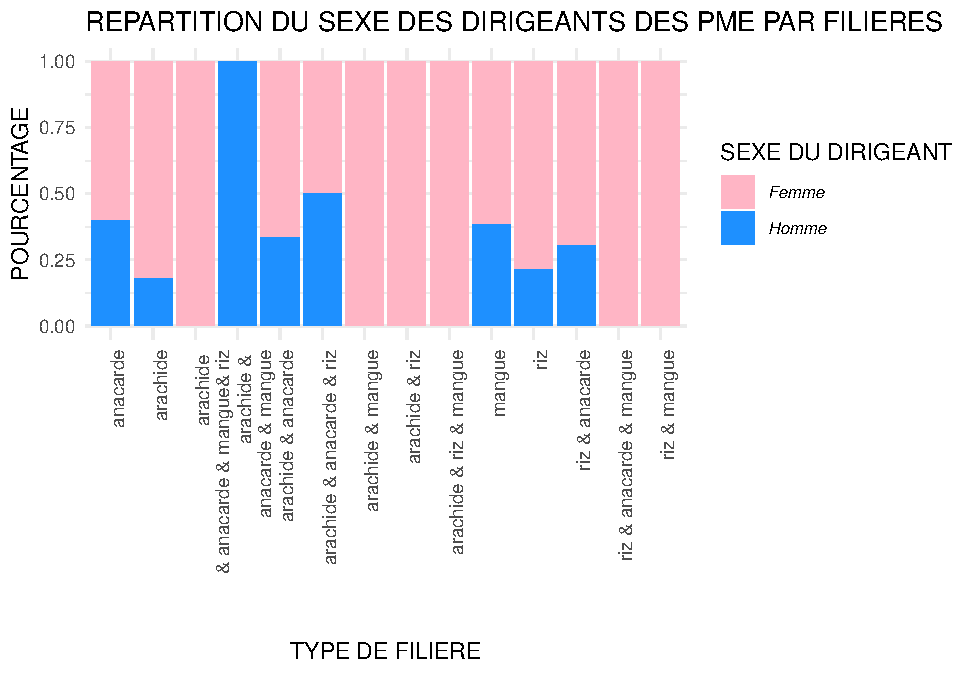
\includegraphics{Projet_R_ISE_1_files/figure-latex/unnamed-chunk-28-1} \end{center}

\hfill\break

\hypertarget{un-regard-sur-la-puxe9riode-de-lenquuxeate}{%
\subparagraph{Un regard sur la période de
l'enquête}\label{un-regard-sur-la-puxe9riode-de-lenquuxeate}}

\hfill\break

\begin{Shaded}
\begin{Highlighting}[]
\CommentTok{\# Couleur personnalisée pour le fond du panneau principal}
\NormalTok{background\_color }\OtherTok{\textless{}{-}} \StringTok{"\#f0f0f0"}

\CommentTok{\# Créer le graphique de densité avec la couleur de fond personnalisée}
\FunctionTok{ggplot}\NormalTok{(projet) }\SpecialCharTok{+}
  \FunctionTok{aes}\NormalTok{(}\AttributeTok{x =}\NormalTok{ today) }\SpecialCharTok{+}
  \FunctionTok{geom\_density}\NormalTok{(}\AttributeTok{fill =} \StringTok{"lightgreen"}\NormalTok{, }
               \AttributeTok{color =} \StringTok{"green"}\NormalTok{, }\AttributeTok{alpha =} \FloatTok{0.2}\NormalTok{) }\SpecialCharTok{+}  \CommentTok{\# Remplissage en  }
                                              \CommentTok{\#bleu avec bordures blanches}
  \FunctionTok{ggtitle}\NormalTok{(}\StringTok{"Période de l’enquête"}\NormalTok{) }\SpecialCharTok{+}
  \FunctionTok{xlab}\NormalTok{(}\StringTok{"Jour de l\textquotesingle{}enquête"}\NormalTok{) }\SpecialCharTok{+}
  \FunctionTok{ylab}\NormalTok{(}\StringTok{"Densité"}\NormalTok{) }\SpecialCharTok{+}
  \FunctionTok{theme\_minimal}\NormalTok{() }\SpecialCharTok{+}
  \FunctionTok{theme}\NormalTok{(}\AttributeTok{panel.background =} \FunctionTok{element\_rect}\NormalTok{(}
    \AttributeTok{fill =}\NormalTok{ background\_color))  }\CommentTok{\# Définir la couleur du }
\end{Highlighting}
\end{Shaded}

\begin{center}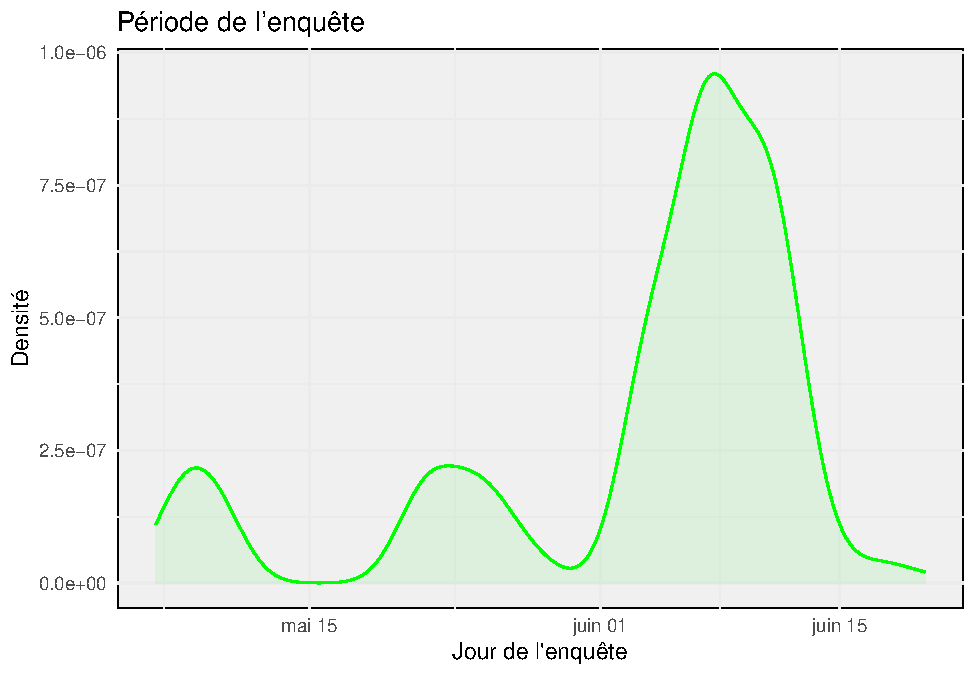
\includegraphics{Projet_R_ISE_1_files/figure-latex/unnamed-chunk-29-1} \end{center}

\begin{Shaded}
\begin{Highlighting}[]
                      \CommentTok{\# fond du panneau principal}
\end{Highlighting}
\end{Shaded}

\hfill\break
Ceci montre que la période d'enquete la plus intense est du 01 juin au
15 juin.

\hfill\break

\hypertarget{analyse-de-luxe2ge-du-dirigeantresponsable-de-la-pme-variable-q24-dans-chaque-filiuxe8re-pour-duxe9terminer-les-tendances-guxe9nuxe9rationnelles.}{%
\subparagraph{Analyse de l'âge du dirigeant/responsable de la PME
(variable q24) dans chaque filière pour déterminer les tendances
générationnelles.}\label{analyse-de-luxe2ge-du-dirigeantresponsable-de-la-pme-variable-q24-dans-chaque-filiuxe8re-pour-duxe9terminer-les-tendances-guxe9nuxe9rationnelles.}}

\hfill\break
On commencera d'abord par filtrer les données pour les âges inférieurs à
100 ans, puisque nous avons à faire à des dirigeants on suppose que ceux
si sont en état de travail, l'age de retraite etant d'un peu plus de
64ans nous prenons donc une marge de +40 ceci nous permet d'eviter de
fausser nos données par des erreurs de saisi comme par exemple saisir un
numero de telephone a la place de l'age

\hfill\break

\begin{Shaded}
\begin{Highlighting}[]
\NormalTok{projet\_filtered }\OtherTok{\textless{}{-}} \FunctionTok{subset}\NormalTok{(projet, Age }\SpecialCharTok{\textless{}} \DecValTok{100}\NormalTok{) }
\CommentTok{\# Défini les couleurs pour les niveaux du sexe}
\NormalTok{couleurs }\OtherTok{\textless{}{-}} \FunctionTok{c}\NormalTok{(}\StringTok{"Femme"} \OtherTok{=} \StringTok{"pink1"}\NormalTok{, }\StringTok{"Homme"} \OtherTok{=} \StringTok{"dodgerblue1"}\NormalTok{)}
\CommentTok{\# Regrouper les âges en catégories}
\NormalTok{projet\_filtered}\SpecialCharTok{$}\NormalTok{Age\_Group }\OtherTok{\textless{}{-}} \FunctionTok{cut}\NormalTok{(projet\_filtered}\SpecialCharTok{$}\NormalTok{Age, }\AttributeTok{breaks =} \FunctionTok{c}\NormalTok{(}\DecValTok{0}\NormalTok{, }\DecValTok{20}\NormalTok{, }\DecValTok{30}\NormalTok{, }
                                                                 \DecValTok{40}\NormalTok{, }\DecValTok{50}\NormalTok{, }\DecValTok{60}\NormalTok{, }
                                                                 \DecValTok{70}\NormalTok{, }\DecValTok{80}\NormalTok{, }\DecValTok{100}\NormalTok{),}
                                 \AttributeTok{labels =} \FunctionTok{c}\NormalTok{(}\StringTok{"0{-}20"}\NormalTok{, }\StringTok{"20{-}30"}\NormalTok{, }\StringTok{"30{-}40"}\NormalTok{,}
                                            \StringTok{"40{-}50"}\NormalTok{, }\StringTok{"50{-}60"}\NormalTok{, }\StringTok{"60{-}70"}\NormalTok{, }
                                            \StringTok{"70{-}80"}\NormalTok{, }\StringTok{"80+"}\NormalTok{))}

\CommentTok{\# Créer la pyramide des âges avec ggplot2}
\NormalTok{pyramide }\OtherTok{\textless{}{-}} \FunctionTok{ggplot}\NormalTok{(projet\_filtered, }\FunctionTok{aes}\NormalTok{(}\AttributeTok{x =}\NormalTok{ Age\_Group, }\AttributeTok{fill =}\NormalTok{ sexe)) }\SpecialCharTok{+}
  \FunctionTok{geom\_bar}\NormalTok{(}\AttributeTok{data =} \FunctionTok{subset}\NormalTok{(projet\_filtered, sexe }\SpecialCharTok{==} \StringTok{"Homme"}\NormalTok{), }
           \FunctionTok{aes}\NormalTok{(}\AttributeTok{y =} \SpecialCharTok{{-}}\NormalTok{..count..),  }\AttributeTok{position =} \StringTok{"dodge"}\NormalTok{) }\SpecialCharTok{+}
  \FunctionTok{geom\_bar}\NormalTok{(}\AttributeTok{data =} \FunctionTok{subset}\NormalTok{(projet\_filtered, sexe }\SpecialCharTok{==} \StringTok{"Femme"}\NormalTok{), }
           \FunctionTok{aes}\NormalTok{(}\AttributeTok{y =}\NormalTok{ ..count..),  }\AttributeTok{position =} \StringTok{"dodge"}\NormalTok{) }\SpecialCharTok{+}
  \FunctionTok{scale\_fill\_manual}\NormalTok{(}\AttributeTok{values =}\NormalTok{ couleurs) }\SpecialCharTok{+}
  \FunctionTok{labs}\NormalTok{(}\AttributeTok{x =} \StringTok{"Âge"}\NormalTok{, }\AttributeTok{y =} \StringTok{"Nombre de personnes"}\NormalTok{, }
       \AttributeTok{title =} \StringTok{"PYRAMIDE PAR CLASSE D\textquotesingle{}AGE"}\NormalTok{) }\SpecialCharTok{+}
  \FunctionTok{theme\_minimal}\NormalTok{() }\SpecialCharTok{+}
  \FunctionTok{coord\_flip}\NormalTok{()}\SpecialCharTok{+}
  \FunctionTok{theme\_light}\NormalTok{()}\SpecialCharTok{+}
  \FunctionTok{theme}\NormalTok{(}\AttributeTok{axis.text.x =} \FunctionTok{element\_text}\NormalTok{(}\AttributeTok{angle =} \DecValTok{45}\NormalTok{, }\AttributeTok{hjust =} \DecValTok{1}\NormalTok{, }
                                   \AttributeTok{vjust =} \DecValTok{1}\NormalTok{, }\AttributeTok{size =} \DecValTok{8}\NormalTok{, }\AttributeTok{color =} \StringTok{"black"}\NormalTok{),}
        \AttributeTok{axis.title =} \FunctionTok{element\_text}\NormalTok{(}\AttributeTok{size=}\DecValTok{8}\NormalTok{, }\AttributeTok{face =} \StringTok{"bold"}\NormalTok{),}
        \AttributeTok{plot.title =} \FunctionTok{element\_text}\NormalTok{(}\AttributeTok{size =} \DecValTok{12}\NormalTok{),}
        \AttributeTok{panel.grid.major.x =} \FunctionTok{element\_blank}\NormalTok{(),}
        \AttributeTok{panel.grid.minor.x =} \FunctionTok{element\_blank}\NormalTok{(),}
        \AttributeTok{panel.grid.major.y =} \FunctionTok{element\_line}\NormalTok{(}\AttributeTok{color =} \StringTok{"green"}\NormalTok{, }\AttributeTok{size =} \FloatTok{0.1}\NormalTok{),}
        \AttributeTok{panel.background =} \FunctionTok{element\_rect}\NormalTok{(}\AttributeTok{fill =} \StringTok{"white"}\NormalTok{))}


\CommentTok{\# Crée du graphique violin}
\NormalTok{Violin}\OtherTok{\textless{}{-}}\FunctionTok{ggplot}\NormalTok{(projet\_filtered, }\FunctionTok{aes}\NormalTok{(}\AttributeTok{x =}\NormalTok{ sexe, }\AttributeTok{y =}\NormalTok{ Age, }\AttributeTok{fill =}\NormalTok{ sexe)) }\SpecialCharTok{+}
  \FunctionTok{geom\_violin}\NormalTok{(}\AttributeTok{alpha =} \FloatTok{0.7}\NormalTok{) }\SpecialCharTok{+}  \CommentTok{\# Opacité pour une meilleure lisibilité des violins}
  \FunctionTok{scale\_fill\_manual}\NormalTok{(}\AttributeTok{values =}\NormalTok{ couleurs) }\SpecialCharTok{+}  \CommentTok{\# Applique les couleurs définies}
  \FunctionTok{xlab}\NormalTok{(}\StringTok{"Sexe"}\NormalTok{) }\SpecialCharTok{+}
  \FunctionTok{ylab}\NormalTok{(}\StringTok{"Âge"}\NormalTok{) }\SpecialCharTok{+}
  \FunctionTok{ggtitle}\NormalTok{(}\StringTok{"REPARTITION DES AGES PAR SEXE"}\NormalTok{) }\SpecialCharTok{+}
  \FunctionTok{theme\_minimal}\NormalTok{() }\SpecialCharTok{+}  \CommentTok{\# Utiliser le thème minimal}
  \FunctionTok{theme\_light}\NormalTok{()}\SpecialCharTok{+}
  \FunctionTok{theme}\NormalTok{(}
    \AttributeTok{plot.background =} \FunctionTok{element\_rect}\NormalTok{(}\AttributeTok{fill =} \StringTok{"white"}\NormalTok{),  }\CommentTok{\# Change la couleur de fond}
    \AttributeTok{panel.grid.major =} \FunctionTok{element\_blank}\NormalTok{(),  }\CommentTok{\# Supprime les lignes de grille majeures}
    \AttributeTok{panel.grid.minor =} \FunctionTok{element\_blank}\NormalTok{()  }\CommentTok{\# Supprime les lignes de grille mineures}
\NormalTok{  )}

\FunctionTok{grid.arrange}\NormalTok{( Violin, pyramide, }\AttributeTok{ncol =} \DecValTok{2}\NormalTok{)}
\end{Highlighting}
\end{Shaded}

\begin{center}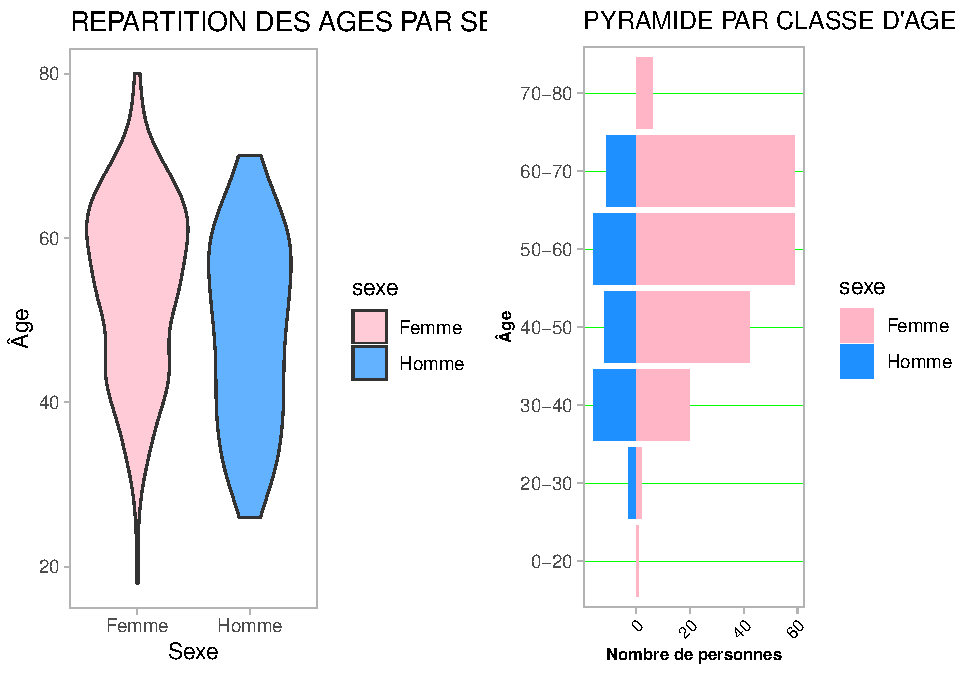
\includegraphics{Projet_R_ISE_1_files/figure-latex/unnamed-chunk-30-1} \end{center}

\hfill\break
Une fois cette observation faites il semble important de se demander
quel est la répartition par Années d'expérience selon le sexe nous
l'alignerons avec un boxplot sur les ages afin de mieux les analyser

\hfill\break

\begin{Shaded}
\begin{Highlighting}[]
\NormalTok{Repartition1 }\OtherTok{=}\NormalTok{ projet }\SpecialCharTok{\%\textgreater{}\%}
\FunctionTok{rename}\NormalTok{(}\AttributeTok{age =}\NormalTok{ q24) }\SpecialCharTok{\%\textgreater{}\%}
\FunctionTok{filter}\NormalTok{( age }\SpecialCharTok{\textless{}} \DecValTok{100}\NormalTok{ )}
\NormalTok{Repartition2 }\OtherTok{=}\NormalTok{ projet }\SpecialCharTok{\%\textgreater{}\%}
\FunctionTok{rename}\NormalTok{(}\AttributeTok{Annees\_experience =}\NormalTok{ q26) }\SpecialCharTok{\%\textgreater{}\%}
  \FunctionTok{filter}\NormalTok{( Annees\_experience }\SpecialCharTok{\textless{}} \DecValTok{50}\NormalTok{ )}
\NormalTok{plot1 }\OtherTok{\textless{}{-}} \FunctionTok{ggplot}\NormalTok{(Repartition1, }\FunctionTok{aes}\NormalTok{(}\AttributeTok{x =}\NormalTok{ sexe, }\AttributeTok{y =}\NormalTok{ age)) }\SpecialCharTok{+}
\FunctionTok{geom\_pirate}\NormalTok{(}\FunctionTok{aes}\NormalTok{(}\AttributeTok{colour =}\NormalTok{ sexe)) }\SpecialCharTok{+}
\FunctionTok{xlab}\NormalTok{(}\StringTok{"Sexe"}\NormalTok{) }\SpecialCharTok{+}
\FunctionTok{ylab}\NormalTok{(}\StringTok{"Âge"}\NormalTok{) }\SpecialCharTok{+}
\FunctionTok{ggtitle}\NormalTok{(}\StringTok{"Répartition par âge selon le sexe"}\NormalTok{) }\SpecialCharTok{+}
\FunctionTok{theme\_light}\NormalTok{()}\SpecialCharTok{+}
\FunctionTok{theme}\NormalTok{(}
\AttributeTok{plot.title =} \FunctionTok{element\_text}\NormalTok{(}\AttributeTok{color =} \StringTok{"black"}\NormalTok{))}
\NormalTok{plot2}\OtherTok{\textless{}{-}} \FunctionTok{ggplot}\NormalTok{(Repartition2, }\FunctionTok{aes}\NormalTok{(}\AttributeTok{x =}\NormalTok{ sexe, }\AttributeTok{y =}\NormalTok{ Annees\_experience)) }\SpecialCharTok{+}
\FunctionTok{geom\_pirate}\NormalTok{(}\FunctionTok{aes}\NormalTok{(}\AttributeTok{colour =}\NormalTok{ sexe)) }\SpecialCharTok{+}
\FunctionTok{xlab}\NormalTok{(}\StringTok{"Sexe"}\NormalTok{) }\SpecialCharTok{+}
\FunctionTok{ylab}\NormalTok{(}\StringTok{"Nombre d\textquotesingle{}années d\textquotesingle{}expérience"}\NormalTok{) }\SpecialCharTok{+}
\FunctionTok{ggtitle}\NormalTok{(}\StringTok{"Années d\textquotesingle{}expérience selon le sexe"}\NormalTok{) }\SpecialCharTok{+}
\FunctionTok{theme\_light}\NormalTok{()}\SpecialCharTok{+}
\FunctionTok{theme}\NormalTok{(}
\AttributeTok{plot.title =} \FunctionTok{element\_text}\NormalTok{(}\AttributeTok{color =} \StringTok{"black"}\NormalTok{))}
\CommentTok{\# Afficher les graphiques côte à côte sur une même ligne}
\FunctionTok{grid.arrange}\NormalTok{(plot1, plot2, }\AttributeTok{ncol =} \DecValTok{2}\NormalTok{)}
\end{Highlighting}
\end{Shaded}

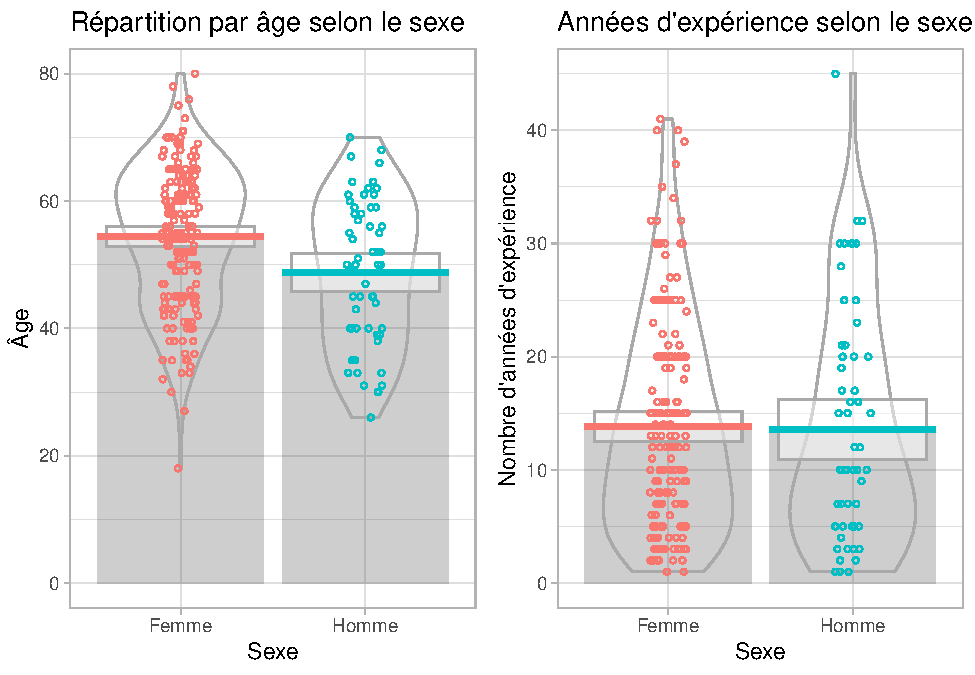
\includegraphics{Projet_R_ISE_1_files/figure-latex/unnamed-chunk-31-1.pdf}\\

\textcolor{blue}{\subsection{ Un peu de cartographie.}}

\textcolor{blue}{\subsubsection{Transformation le data.frame en données géographiques dont l'objet sera nommé projetmap.}}

\hfill\break

\begin{Shaded}
\begin{Highlighting}[]
\CommentTok{\# Création de l\textquotesingle{}objet projet\_map avec des données géographiques}
\NormalTok{projet\_map }\OtherTok{\textless{}{-}}\NormalTok{ projet }\SpecialCharTok{\%\textgreater{}\%}
  \FunctionTok{st\_as\_sf}\NormalTok{(}\AttributeTok{coords =} \FunctionTok{c}\NormalTok{(}\StringTok{"gps\_menlongitude"}\NormalTok{, }\StringTok{"gps\_menlatitude"}\NormalTok{), }\AttributeTok{crs =} \DecValTok{4326}\NormalTok{)}
\CommentTok{\#Ceci provient du referentiel mondiale}
\end{Highlighting}
\end{Shaded}

\hfill\break

\textcolor{blue}{\subsubsection{Réprésentation spatiale des PME suivant le sexe.}}

\hfill\break

\hypertarget{cruxe9ation-de-la-carte-spatiale-des-pme-selon-le-sexe}{%
\paragraph{Création de la carte spatiale des PME selon le
sexe}\label{cruxe9ation-de-la-carte-spatiale-des-pme-selon-le-sexe}}

\hfill\break

\begin{center}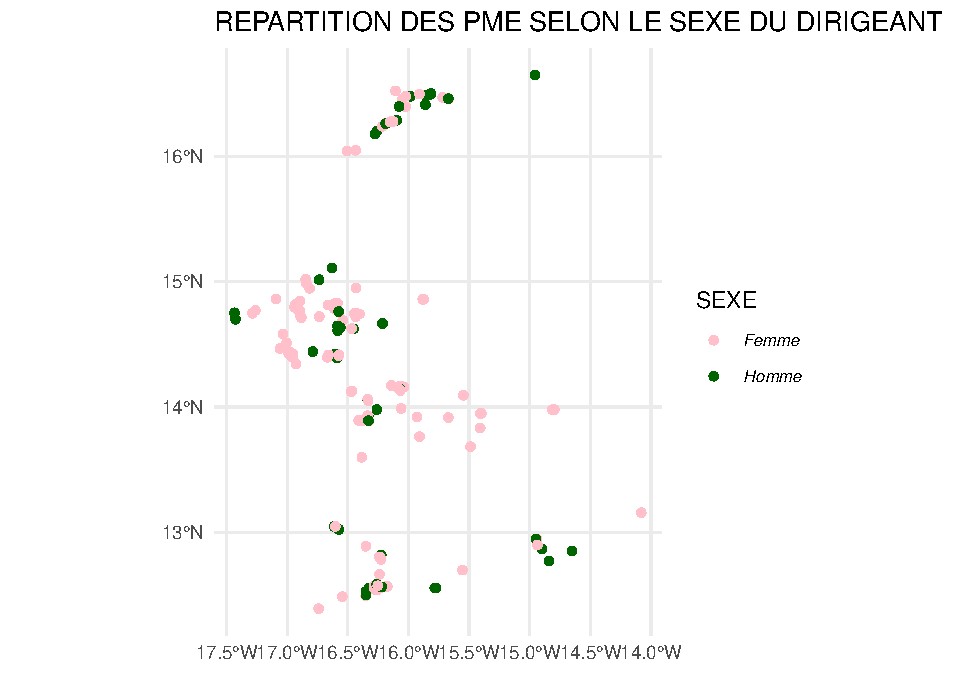
\includegraphics{Projet_R_ISE_1_files/figure-latex/unnamed-chunk-33-1} \end{center}

\hfill\break
Pour une meilleure presentation ajoutons la carte du sénégal\\

\hypertarget{chargement-des-coordonnuxe9es-guxe9ographiques-de-la-ruxe9gion-du-pays}{%
\paragraph{Chargement des coordonnées géographiques de la région du
pays}\label{chargement-des-coordonnuxe9es-guxe9ographiques-de-la-ruxe9gion-du-pays}}

\hfill\break

\begin{Shaded}
\begin{Highlighting}[]
\CommentTok{\# Chargement des coordonnées géographiques de la région du pays}
\NormalTok{occ\_raw }\OtherTok{\textless{}{-}} \FunctionTok{st\_read}\NormalTok{(}\AttributeTok{dsn =} \StringTok{"data/sen.gpkg"}\NormalTok{, }\AttributeTok{stringsAsFactors =} \ConstantTok{FALSE}\NormalTok{)}
\end{Highlighting}
\end{Shaded}

\begin{verbatim}
## Multiple layers are present in data source C:\Users\HP\Desktop\moi 22-23\sm2\R\Durel_Valdes_NZIALI_TCHAMOU\data\sen.gpkg, reading layer `sen_adm3'.
## Use `st_layers' to list all layer names and their type in a data source.
## Set the `layer' argument in `st_read' to read a particular layer.
## Reading layer `sen_adm3' from data source 
##   `C:\Users\HP\Desktop\moi 22-23\sm2\R\Durel_Valdes_NZIALI_TCHAMOU\data\sen.gpkg' 
##   using driver `GPKG'
## Simple feature collection with 121 features and 8 fields
## Geometry type: MULTIPOLYGON
## Dimension:     XY
## Bounding box:  xmin: -17.53092 ymin: 12.30777 xmax: -11.34801 ymax: 16.69373
## Geodetic CRS:  WGS 84
\end{verbatim}

\begin{Shaded}
\begin{Highlighting}[]
\NormalTok{occ }\OtherTok{\textless{}{-}} \FunctionTok{st\_transform}\NormalTok{(}\AttributeTok{x =}\NormalTok{ occ\_raw, }\AttributeTok{crs =} \DecValTok{4326}\NormalTok{)}

\NormalTok{OCCreg}\OtherTok{\textless{}{-}}\NormalTok{occ }\SpecialCharTok{\%\textgreater{}\%} 
\NormalTok{          dplyr}\SpecialCharTok{::}\FunctionTok{select}\NormalTok{(adm1\_id,adm1\_name, adm0\_id,adm0\_name,geom )}\SpecialCharTok{\%\textgreater{}\%} 
              \FunctionTok{group\_by}\NormalTok{(adm1\_id,adm1\_name, adm0\_id,adm0\_name) }\SpecialCharTok{\%\textgreater{}\%} 
                  \FunctionTok{summarise}\NormalTok{(}\FunctionTok{sum}\NormalTok{())}
\end{Highlighting}
\end{Shaded}

\hfill\break

\hypertarget{cruxe9ation-de-la-carte-spatiale-des-pme-selon-le-sexe-et-la-ruxe9gion-avec-la-ruxe9gion-en-arriuxe8re-plan}{%
\paragraph{Création de la carte spatiale des PME selon le sexe et la
région avec la région en
arrière-plan}\label{cruxe9ation-de-la-carte-spatiale-des-pme-selon-le-sexe-et-la-ruxe9gion-avec-la-ruxe9gion-en-arriuxe8re-plan}}

\hfill\break

\begin{Shaded}
\begin{Highlighting}[]
\CommentTok{\# Création de la carte spatiale des PME selon le sexe et la région }
\FunctionTok{ggplot}\NormalTok{() }\SpecialCharTok{+}
  \FunctionTok{geom\_sf}\NormalTok{(}\AttributeTok{data =}\NormalTok{ OCCreg, }
          \AttributeTok{color =} \StringTok{"lightgreen"}\NormalTok{) }\SpecialCharTok{+}  \CommentTok{\# Carte de la région en arrière{-}plan}
  \FunctionTok{geom\_sf\_label}\NormalTok{(}\AttributeTok{data =}\NormalTok{ OCCreg, }\FunctionTok{aes}\NormalTok{(}\AttributeTok{label =}\NormalTok{ adm1\_name),}
                \AttributeTok{color =} \StringTok{"darkred"}\NormalTok{, }\AttributeTok{size =} \DecValTok{2}\NormalTok{)}\SpecialCharTok{+}
  \FunctionTok{coord\_sf}\NormalTok{() }\SpecialCharTok{+}
  \FunctionTok{geom\_sf}\NormalTok{(}\AttributeTok{data =}\NormalTok{ projet\_map, }\FunctionTok{aes}\NormalTok{(}\AttributeTok{color =}\NormalTok{ sexe)) }\SpecialCharTok{+}
  \FunctionTok{scale\_color\_manual}\NormalTok{(}
    \AttributeTok{values =} \FunctionTok{c}\NormalTok{(}\StringTok{"blue"}\NormalTok{, }\StringTok{"lightpink"}\NormalTok{)) }\SpecialCharTok{+}  \CommentTok{\# Couleurs des catégories de sexe }
  \FunctionTok{labs}\NormalTok{(}\AttributeTok{color =} \StringTok{"GENRE"}\NormalTok{) }\SpecialCharTok{+}
  \FunctionTok{theme\_minimal}\NormalTok{()}\SpecialCharTok{+}
  \FunctionTok{theme}\NormalTok{(}\AttributeTok{legend.text =} \FunctionTok{element\_text}\NormalTok{(}\AttributeTok{face =} \StringTok{"italic"}\NormalTok{, }\AttributeTok{size =} \DecValTok{8}\NormalTok{))}\SpecialCharTok{+}
  \FunctionTok{theme}\NormalTok{(}\AttributeTok{panel.background =} \FunctionTok{element\_rect}\NormalTok{(}\AttributeTok{fill =} \StringTok{"azure"}\NormalTok{,}\AttributeTok{color=}\ConstantTok{NA}\NormalTok{)) }\SpecialCharTok{+}
  \FunctionTok{annotation\_north\_arrow}\NormalTok{(}
    \AttributeTok{location =} \StringTok{"tl"}\NormalTok{, }\AttributeTok{which\_north =} \StringTok{"true"}\NormalTok{, }\AttributeTok{style =}\NormalTok{ north\_arrow\_orienteering)}\SpecialCharTok{+}
  \FunctionTok{annotation\_scale}\NormalTok{(}\AttributeTok{location =} \StringTok{"bl"}\NormalTok{, }\AttributeTok{width\_hint =} \FloatTok{0.2}\NormalTok{)}\SpecialCharTok{+}
  \FunctionTok{labs}\NormalTok{(}\AttributeTok{title =} \StringTok{"REPARTITION DES PME SELON LE GENRE DU DIRIGEANT"}\NormalTok{)}
\end{Highlighting}
\end{Shaded}

\begin{center}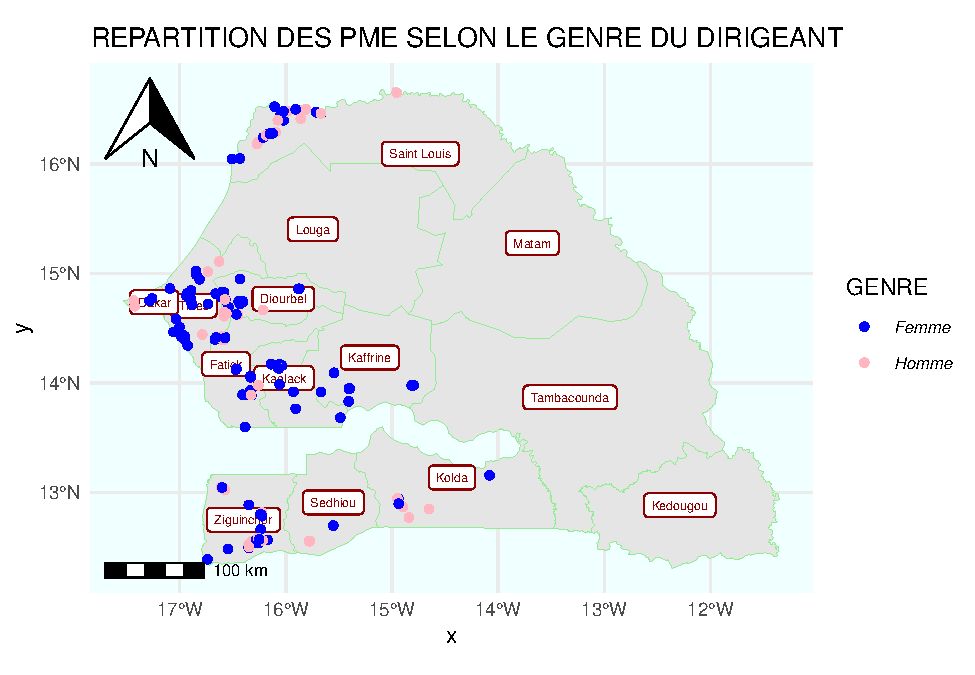
\includegraphics{Projet_R_ISE_1_files/figure-latex/unnamed-chunk-35-1} \end{center}

\hfill\break

\textcolor{blue}{\subsubsection{Faites une réprésentation spatiale des PME suivant le niveau d'instruction.}}

\hfill\break

\begin{Shaded}
\begin{Highlighting}[]
\CommentTok{\# Création de la carte spatiale des PME selon le sexe}
\FunctionTok{ggplot}\NormalTok{() }\SpecialCharTok{+}
  \FunctionTok{geom\_sf}\NormalTok{(}\AttributeTok{data =}\NormalTok{ OCCreg, }\AttributeTok{color =} \StringTok{"lightgreen"}\NormalTok{) }\SpecialCharTok{+}  \CommentTok{\# Carte de la région en arrière{-}plan}
  \FunctionTok{geom\_sf\_label}\NormalTok{(}\AttributeTok{data =}\NormalTok{ OCCreg, }\FunctionTok{aes}\NormalTok{(}\AttributeTok{label =}\NormalTok{ adm1\_name), }\AttributeTok{color =} \StringTok{"darkred"}\NormalTok{, }\AttributeTok{size =} \DecValTok{2}\NormalTok{)}\SpecialCharTok{+}
  \FunctionTok{coord\_sf}\NormalTok{() }\SpecialCharTok{+}
  \FunctionTok{geom\_sf}\NormalTok{(}\AttributeTok{data =}\NormalTok{ projet\_map, }\FunctionTok{aes}\NormalTok{(}\AttributeTok{color =}\NormalTok{ q25)) }\SpecialCharTok{+}
  \FunctionTok{scale\_fill\_manual}\NormalTok{(}
    \AttributeTok{values =} \FunctionTok{c}\NormalTok{(}\StringTok{"\#E45756"}\NormalTok{, }\StringTok{"\#4C78A8"}\NormalTok{,}\StringTok{"darkgreen"}\NormalTok{,}\StringTok{"blue"}\NormalTok{)) }\SpecialCharTok{+}  \CommentTok{\# Couleurs des  }
  \FunctionTok{labs}\NormalTok{(}\AttributeTok{color =} \StringTok{"NIVEAU ACADEMIQUE"}\NormalTok{) }\SpecialCharTok{+}                       \CommentTok{\#catégories de sex}
  \FunctionTok{theme\_minimal}\NormalTok{()}\SpecialCharTok{+}
  \FunctionTok{theme}\NormalTok{(}\AttributeTok{legend.text =} \FunctionTok{element\_text}\NormalTok{(}\AttributeTok{face =} \StringTok{"italic"}\NormalTok{, }\AttributeTok{size =} \DecValTok{8}\NormalTok{))}\SpecialCharTok{+}
  \FunctionTok{theme}\NormalTok{(}\AttributeTok{panel.background =} \FunctionTok{element\_rect}\NormalTok{(}\AttributeTok{fill =} \StringTok{"azure"}\NormalTok{,}\AttributeTok{color=}\ConstantTok{NA}\NormalTok{)) }\SpecialCharTok{+}
  \FunctionTok{annotation\_north\_arrow}\NormalTok{(}
    \AttributeTok{location =} \StringTok{"tl"}\NormalTok{, }\AttributeTok{which\_north =} \StringTok{"true"}\NormalTok{, }\AttributeTok{style =}\NormalTok{ north\_arrow\_orienteering)}\SpecialCharTok{+}
  \FunctionTok{annotation\_scale}\NormalTok{(}\AttributeTok{location =} \StringTok{"bl"}\NormalTok{, }\AttributeTok{width\_hint =} \FloatTok{0.2}\NormalTok{)}\SpecialCharTok{+}
  \FunctionTok{labs}\NormalTok{(}\AttributeTok{title =} \StringTok{"REPARTITION DES PME PAR LE NIVEAU D\textquotesingle{}INSTRUCTION DES DIRIGEANTS"}\NormalTok{)}
\end{Highlighting}
\end{Shaded}

\begin{center}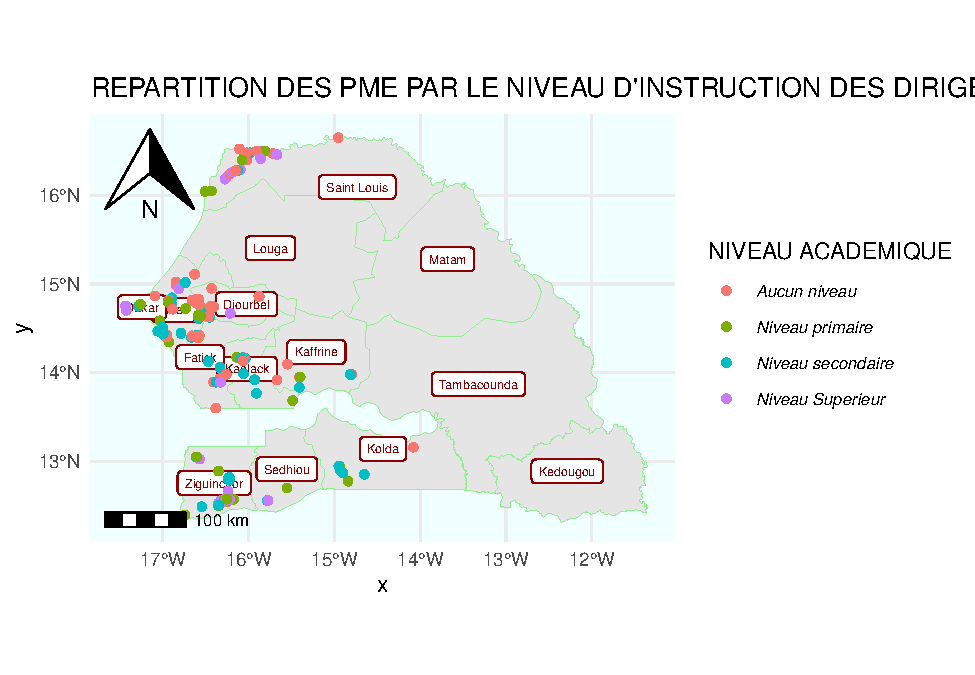
\includegraphics{Projet_R_ISE_1_files/figure-latex/unnamed-chunk-36-1} \end{center}

\hfill\break

\textcolor{blue}{\subsubsection{Analyse spatiale de choix.}}

\hfill\break

\hypertarget{ruxe9partition-guxe9ographiquedes-pme-selon-le-nombre-de-filiuxe8res-quelle-possuxe8de}{%
\paragraph{Répartition géographiquedes PME selon le nombre de filières
quelle
possède}\label{ruxe9partition-guxe9ographiquedes-pme-selon-le-nombre-de-filiuxe8res-quelle-possuxe8de}}

\hfill\break

\begin{Shaded}
\begin{Highlighting}[]
\CommentTok{\# répartition géographiquedes PME selon les filiere}
\FunctionTok{ggplot}\NormalTok{() }\SpecialCharTok{+}
  \FunctionTok{geom\_sf}\NormalTok{(}\AttributeTok{data =}\NormalTok{ OCCreg, }\AttributeTok{color =} \StringTok{"lightgreen"}\NormalTok{) }\SpecialCharTok{+}  
  \FunctionTok{geom\_sf\_label}\NormalTok{(}\AttributeTok{data =}\NormalTok{ OCCreg, }
                \FunctionTok{aes}\NormalTok{(}\AttributeTok{label =}\NormalTok{ adm1\_name), }\AttributeTok{color =} \StringTok{"darkred"}\NormalTok{, }\AttributeTok{size =} \DecValTok{2}\NormalTok{)}\SpecialCharTok{+}
  \FunctionTok{coord\_sf}\NormalTok{() }\SpecialCharTok{+}
  \FunctionTok{geom\_sf}\NormalTok{(}\AttributeTok{data =}\NormalTok{ projet\_map, }\FunctionTok{aes}\NormalTok{(}\AttributeTok{color =}\NormalTok{ filiere)) }\SpecialCharTok{+}
  \FunctionTok{scale\_fill\_manual}\NormalTok{(}\AttributeTok{values =} \FunctionTok{c}\NormalTok{(}\StringTok{"\#E45756"}\NormalTok{, }\StringTok{"\#4C78A8"}\NormalTok{,}\StringTok{"darkgreen"}\NormalTok{,}\StringTok{"blue"}\NormalTok{)) }\SpecialCharTok{+} 
  \FunctionTok{labs}\NormalTok{(}\AttributeTok{color =} \StringTok{"NOMBRE DE FILIERES"}\NormalTok{) }\SpecialCharTok{+}
  \FunctionTok{theme\_minimal}\NormalTok{()}\SpecialCharTok{+}
  \FunctionTok{theme}\NormalTok{(}\AttributeTok{legend.text =} \FunctionTok{element\_text}\NormalTok{(}\AttributeTok{face =} \StringTok{"italic"}\NormalTok{, }\AttributeTok{size =} \DecValTok{8}\NormalTok{))}\SpecialCharTok{+}
  \FunctionTok{theme}\NormalTok{(}\AttributeTok{panel.background =} \FunctionTok{element\_rect}\NormalTok{(}\AttributeTok{fill =} \StringTok{"azure"}\NormalTok{,}\AttributeTok{color=}\ConstantTok{NA}\NormalTok{)) }\SpecialCharTok{+}
  \FunctionTok{annotation\_north\_arrow}\NormalTok{(}
    \AttributeTok{location =} \StringTok{"tl"}\NormalTok{, }\AttributeTok{which\_north =} \StringTok{"true"}\NormalTok{, }\AttributeTok{style =}\NormalTok{ north\_arrow\_orienteering)}\SpecialCharTok{+}
  \FunctionTok{annotation\_scale}\NormalTok{(}\AttributeTok{location =} \StringTok{"bl"}\NormalTok{, }\AttributeTok{width\_hint =} \FloatTok{0.2}\NormalTok{)}\SpecialCharTok{+}
  \FunctionTok{labs}\NormalTok{(}\AttributeTok{title =} \StringTok{"REPARTITION DES PME SELON LE NOMBRE DE FILIERES"}\NormalTok{)}
\end{Highlighting}
\end{Shaded}

\begin{center}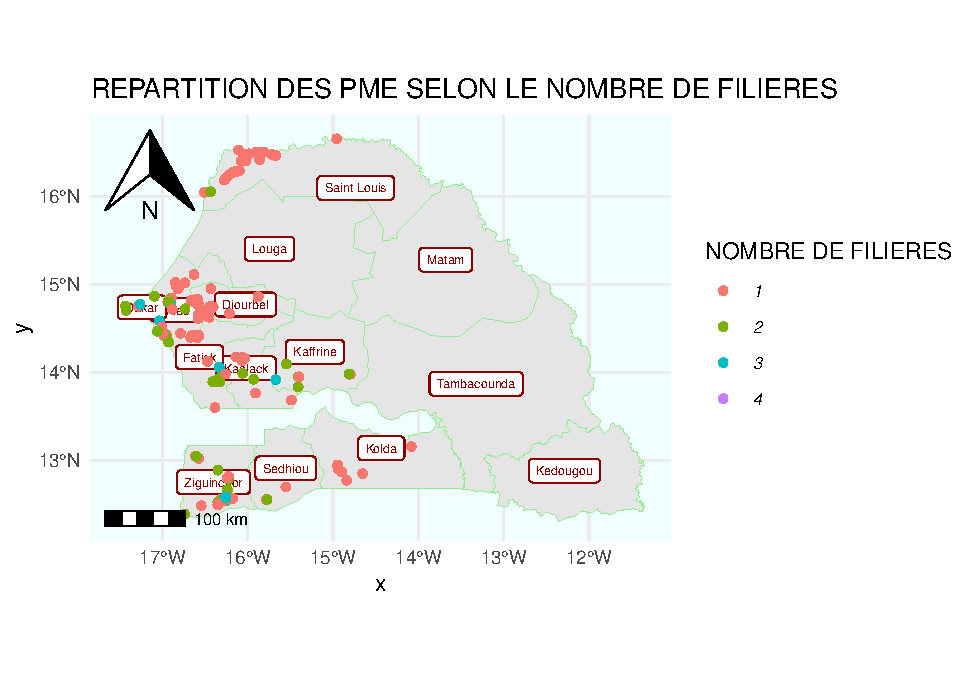
\includegraphics{Projet_R_ISE_1_files/figure-latex/unnamed-chunk-37-1} \end{center}

\hfill\break

Commencons donc à filtrer notre carte\\

\hypertarget{ruxe9partition-guxe9ographiquedes-pme-qui-font-dans-une-seule-culture}{%
\paragraph{Répartition géographiquedes PME qui font dans une seule
culture}\label{ruxe9partition-guxe9ographiquedes-pme-qui-font-dans-une-seule-culture}}

\hfill\break

\begin{Shaded}
\begin{Highlighting}[]
\CommentTok{\# répartition géographiquedes PME qui font dans une seule culture}
\CommentTok{\# filtre les PME qui font dans une seule filiere}
\NormalTok{projet\_map1}\OtherTok{\textless{}{-}}\NormalTok{projet\_map }\SpecialCharTok{\%\textgreater{}\%} \FunctionTok{filter}\NormalTok{(filiere}\SpecialCharTok{==}\DecValTok{1}\NormalTok{) }
 \CommentTok{\# Carte de la région en arrière{-}plan}
\FunctionTok{ggplot}\NormalTok{() }\SpecialCharTok{+}
  \FunctionTok{geom\_sf}\NormalTok{(}\AttributeTok{data =}\NormalTok{ OCCreg, }\AttributeTok{color =} \StringTok{"lightgreen"}\NormalTok{) }\SpecialCharTok{+} 
  \FunctionTok{geom\_sf\_label}\NormalTok{(}\AttributeTok{data =}\NormalTok{ OCCreg, }
                \FunctionTok{aes}\NormalTok{(}\AttributeTok{label =}\NormalTok{ adm1\_name), }\AttributeTok{color =} \StringTok{"darkred"}\NormalTok{, }\AttributeTok{size =} \DecValTok{2}\NormalTok{)}\SpecialCharTok{+}
  \FunctionTok{coord\_sf}\NormalTok{() }\SpecialCharTok{+}
  \FunctionTok{geom\_sf}\NormalTok{(}\AttributeTok{data =}\NormalTok{ projet\_map1, }\FunctionTok{aes}\NormalTok{(}\AttributeTok{color =}\NormalTok{ nom\_filiere)) }\SpecialCharTok{+}
  \FunctionTok{scale\_fill\_manual}\NormalTok{(}\AttributeTok{values =} \FunctionTok{c}\NormalTok{(}\StringTok{"\#E45756"}\NormalTok{, }\StringTok{"\#4C78A8"}\NormalTok{,}\StringTok{"darkgreen"}\NormalTok{,}\StringTok{"blue"}\NormalTok{)) }\SpecialCharTok{+} 
  \FunctionTok{labs}\NormalTok{(}\AttributeTok{color =} \StringTok{"FILIERE"}\NormalTok{) }\SpecialCharTok{+}
  \FunctionTok{theme\_minimal}\NormalTok{()}\SpecialCharTok{+}
  \FunctionTok{theme}\NormalTok{(}\AttributeTok{legend.text =} \FunctionTok{element\_text}\NormalTok{(}\AttributeTok{face =} \StringTok{"italic"}\NormalTok{, }\AttributeTok{size =} \DecValTok{8}\NormalTok{))}\SpecialCharTok{+}
  \FunctionTok{theme}\NormalTok{(}\AttributeTok{panel.background =} \FunctionTok{element\_rect}\NormalTok{(}\AttributeTok{fill =} \StringTok{"azure"}\NormalTok{,}\AttributeTok{color=}\ConstantTok{NA}\NormalTok{)) }\SpecialCharTok{+}
  \FunctionTok{annotation\_north\_arrow}\NormalTok{(}
    \AttributeTok{location =} \StringTok{"tl"}\NormalTok{, }\AttributeTok{which\_north =} \StringTok{"true"}\NormalTok{, }\AttributeTok{style =}\NormalTok{ north\_arrow\_orienteering)}\SpecialCharTok{+}
  \FunctionTok{annotation\_scale}\NormalTok{(}\AttributeTok{location =} \StringTok{"bl"}\NormalTok{, }\AttributeTok{width\_hint =} \FloatTok{0.2}\NormalTok{)}\SpecialCharTok{+}
  \FunctionTok{labs}\NormalTok{(}\AttributeTok{title =} \StringTok{"REPARTITION GEOGRAPHIQUE DES PME SELON LES FILIERES"}\NormalTok{)}
\end{Highlighting}
\end{Shaded}

\begin{center}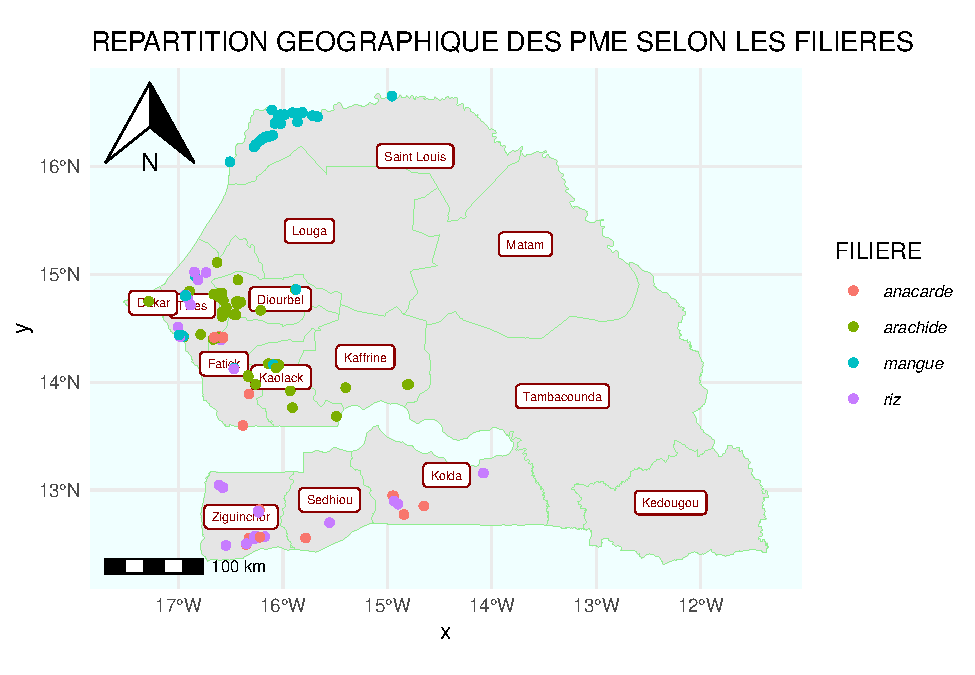
\includegraphics{Projet_R_ISE_1_files/figure-latex/unnamed-chunk-38-1} \end{center}

\hfill\break

\hypertarget{ruxe9partition-guxe9ographique-des-pme-qui-font-dans-deux-culture}{%
\paragraph{Répartition géographique des PME qui font dans deux
culture}\label{ruxe9partition-guxe9ographique-des-pme-qui-font-dans-deux-culture}}

\hfill\break

\begin{Shaded}
\begin{Highlighting}[]
\CommentTok{\# répartition géographiquedes PME qui font dans deux  cultures}
 \CommentTok{\# filtre les PME qui font dans deux filieres}
\NormalTok{projet\_map1}\OtherTok{\textless{}{-}}\NormalTok{projet\_map }\SpecialCharTok{\%\textgreater{}\%} \FunctionTok{filter}\NormalTok{(filiere}\SpecialCharTok{==}\DecValTok{2}\NormalTok{)}
\FunctionTok{ggplot}\NormalTok{() }\SpecialCharTok{+}
  \FunctionTok{geom\_sf}\NormalTok{(}\AttributeTok{data =}\NormalTok{ OCCreg, }\AttributeTok{color =} \StringTok{"lightgreen"}\NormalTok{) }\SpecialCharTok{+} 
  \FunctionTok{geom\_sf\_label}\NormalTok{(}\AttributeTok{data =}\NormalTok{ OCCreg, }
                \FunctionTok{aes}\NormalTok{(}\AttributeTok{label =}\NormalTok{ adm1\_name), }\AttributeTok{color =} \StringTok{"darkred"}\NormalTok{, }\AttributeTok{size =} \DecValTok{2}\NormalTok{)}\SpecialCharTok{+}
  \FunctionTok{coord\_sf}\NormalTok{() }\SpecialCharTok{+}
  \FunctionTok{geom\_sf}\NormalTok{(}\AttributeTok{data =}\NormalTok{ projet\_map1, }\FunctionTok{aes}\NormalTok{(}\AttributeTok{color =}\NormalTok{ nom\_filiere)) }\SpecialCharTok{+}
  \FunctionTok{scale\_fill\_manual}\NormalTok{(}\AttributeTok{values =} \FunctionTok{c}\NormalTok{(}\StringTok{"\#E45756"}\NormalTok{, }\StringTok{"\#4C78A8"}\NormalTok{,}\StringTok{"darkgreen"}\NormalTok{,}\StringTok{"blue"}\NormalTok{)) }\SpecialCharTok{+}  
  \FunctionTok{labs}\NormalTok{(}\AttributeTok{color =} \StringTok{"FILIERE"}\NormalTok{) }\SpecialCharTok{+}
  \FunctionTok{theme\_minimal}\NormalTok{()}\SpecialCharTok{+}
  \FunctionTok{theme}\NormalTok{(}\AttributeTok{legend.text =} \FunctionTok{element\_text}\NormalTok{(}\AttributeTok{face =} \StringTok{"italic"}\NormalTok{, }\AttributeTok{size =} \DecValTok{8}\NormalTok{))}\SpecialCharTok{+}
  \FunctionTok{theme}\NormalTok{(}\AttributeTok{panel.background =} \FunctionTok{element\_rect}\NormalTok{(}\AttributeTok{fill =} \StringTok{"azure"}\NormalTok{,}\AttributeTok{color=}\ConstantTok{NA}\NormalTok{)) }\SpecialCharTok{+}
  \FunctionTok{annotation\_north\_arrow}\NormalTok{(}
    \AttributeTok{location =} \StringTok{"tl"}\NormalTok{, }\AttributeTok{which\_north =} \StringTok{"true"}\NormalTok{, }\AttributeTok{style =}\NormalTok{ north\_arrow\_orienteering)}\SpecialCharTok{+}
  \FunctionTok{annotation\_scale}\NormalTok{(}\AttributeTok{location =} \StringTok{"bl"}\NormalTok{, }\AttributeTok{width\_hint =} \FloatTok{0.2}\NormalTok{)}\SpecialCharTok{+}
  \FunctionTok{labs}\NormalTok{(}\AttributeTok{title =} \StringTok{"REPARTITION GEOGRAPHIQUE DES PME SELON LES FILIERES"}\NormalTok{)}
\end{Highlighting}
\end{Shaded}

\begin{center}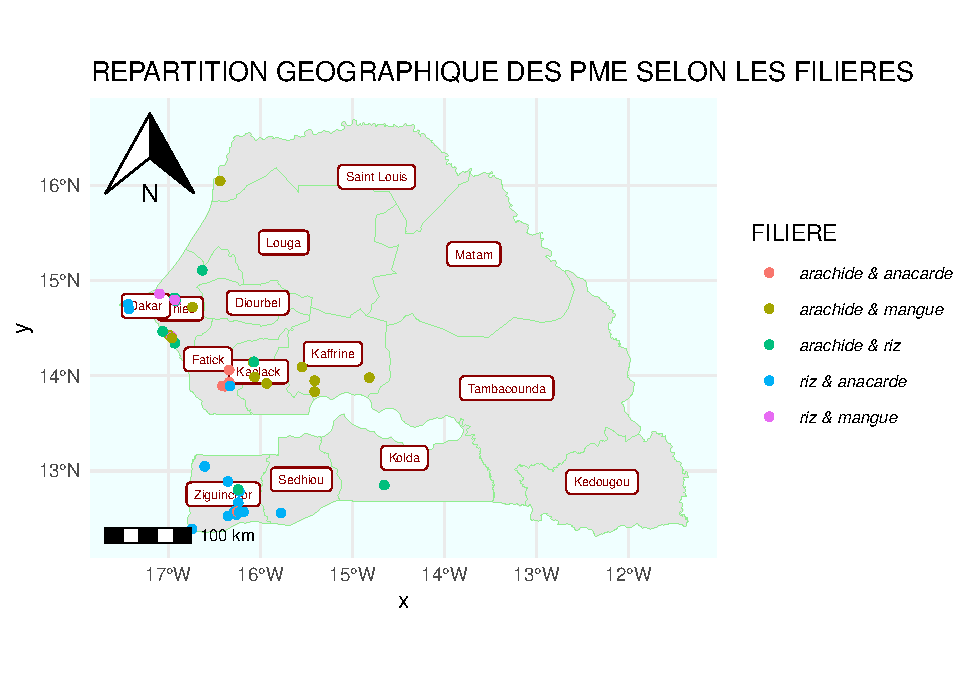
\includegraphics{Projet_R_ISE_1_files/figure-latex/unnamed-chunk-39-1} \end{center}

\hfill\break

\hypertarget{ruxe9partition-guxe9ographique-des-pme-qui-font-dans-trois-cultures}{%
\paragraph{Répartition géographique des PME qui font dans trois
cultures}\label{ruxe9partition-guxe9ographique-des-pme-qui-font-dans-trois-cultures}}

\hfill\break

\begin{Shaded}
\begin{Highlighting}[]
\CommentTok{\# répartition géographiquedes PME qui font dans trois  cultures}
\CommentTok{\# filtre les PME qui font dans trois filieres}
\NormalTok{projet\_map1}\OtherTok{\textless{}{-}}\NormalTok{projet\_map }\SpecialCharTok{\%\textgreater{}\%} \FunctionTok{filter}\NormalTok{(filiere}\SpecialCharTok{==}\DecValTok{3}\SpecialCharTok{|}\NormalTok{ filiere }\SpecialCharTok{==} \DecValTok{4}\NormalTok{)}
\CommentTok{\# Carte de la région en arrière{-}plan}
\FunctionTok{ggplot}\NormalTok{() }\SpecialCharTok{+}
  \FunctionTok{geom\_sf}\NormalTok{(}\AttributeTok{data =}\NormalTok{ OCCreg, }\AttributeTok{color =} \StringTok{"lightgreen"}\NormalTok{) }\SpecialCharTok{+}  
  \FunctionTok{geom\_sf\_label}\NormalTok{(}\AttributeTok{data =}\NormalTok{ OCCreg, }\FunctionTok{aes}\NormalTok{(}\AttributeTok{label =}\NormalTok{ adm1\_name), }\AttributeTok{color =} \StringTok{"darkred"}\NormalTok{, }\AttributeTok{size =} \DecValTok{2}\NormalTok{)}\SpecialCharTok{+}
  \FunctionTok{coord\_sf}\NormalTok{() }\SpecialCharTok{+}
  \FunctionTok{geom\_sf}\NormalTok{(}\AttributeTok{data =}\NormalTok{ projet\_map1, }\FunctionTok{aes}\NormalTok{(}\AttributeTok{color =}\NormalTok{ nom\_filiere)) }\SpecialCharTok{+}
  \FunctionTok{scale\_fill\_manual}\NormalTok{(}\AttributeTok{values =} \FunctionTok{c}\NormalTok{(}\StringTok{"\#E45756"}\NormalTok{, }\StringTok{"\#4C78A8"}\NormalTok{,}\StringTok{"darkgreen"}\NormalTok{,}\StringTok{"blue"}\NormalTok{)) }\SpecialCharTok{+} 
  \FunctionTok{labs}\NormalTok{(}\AttributeTok{color =} \StringTok{"FILIERE"}\NormalTok{) }\SpecialCharTok{+}
  \FunctionTok{theme\_minimal}\NormalTok{()}\SpecialCharTok{+}\FunctionTok{theme}\NormalTok{(}\AttributeTok{legend.text =} \FunctionTok{element\_text}\NormalTok{(}\AttributeTok{face =} \StringTok{"italic"}\NormalTok{, }\AttributeTok{size =} \DecValTok{7}\NormalTok{))}\SpecialCharTok{+}
  \FunctionTok{theme}\NormalTok{(}\AttributeTok{panel.background =} \FunctionTok{element\_rect}\NormalTok{(}\AttributeTok{fill =} \StringTok{"azure"}\NormalTok{,}\AttributeTok{color=}\ConstantTok{NA}\NormalTok{)) }\SpecialCharTok{+}
  \FunctionTok{annotation\_north\_arrow}\NormalTok{(}\AttributeTok{location =} \StringTok{"tl"}\NormalTok{, }\AttributeTok{which\_north =} \StringTok{"true"}\NormalTok{, }\AttributeTok{style =}\NormalTok{ north\_arrow\_orienteering)}\SpecialCharTok{+}
  \FunctionTok{annotation\_scale}\NormalTok{(}\AttributeTok{location =} \StringTok{"bl"}\NormalTok{, }\AttributeTok{width\_hint =} \FloatTok{0.2}\NormalTok{)}\SpecialCharTok{+}
  \FunctionTok{labs}\NormalTok{(}\AttributeTok{title =} \StringTok{"REPARTITION GEOGRAPHIQUE DES PME SELON LES FILIERES"}\NormalTok{)}
\end{Highlighting}
\end{Shaded}

\begin{center}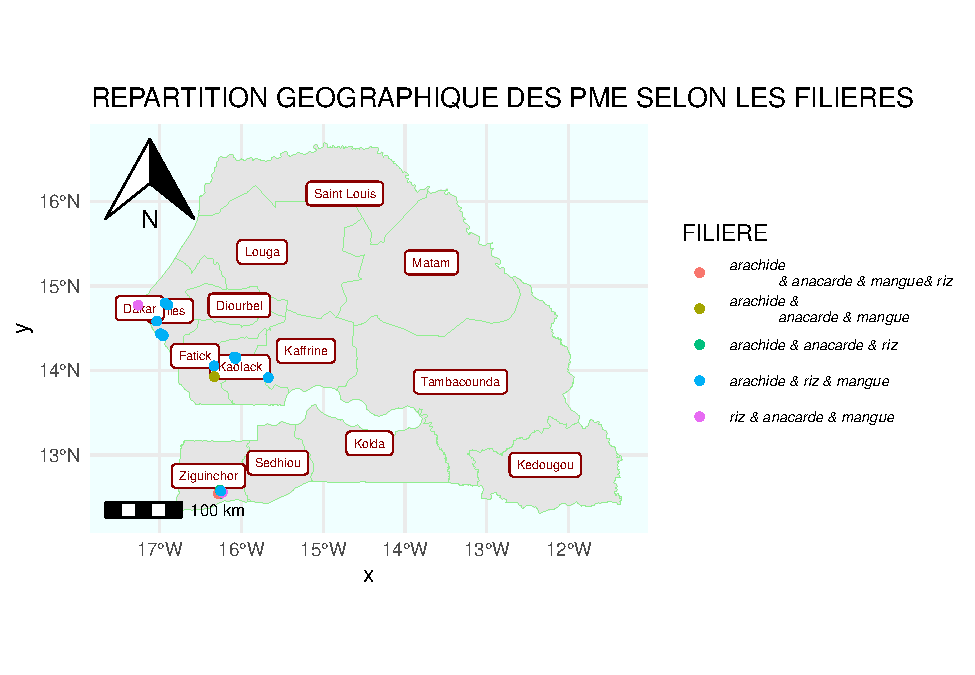
\includegraphics{Projet_R_ISE_1_files/figure-latex/unnamed-chunk-40-1} \end{center}

\hfill\break

\hypertarget{uxe9valuation-des-pme-de-chaque-filiuxe8re-qui-sont-desservies-par-des-routes-bitumuxe9es-et-examination-de-luxe9tat-de-ces-routes.}{%
\paragraph{Évaluation des PME de chaque filière qui sont desservies par
des routes bitumées et examination de l'état de ces
routes.}\label{uxe9valuation-des-pme-de-chaque-filiuxe8re-qui-sont-desservies-par-des-routes-bitumuxe9es-et-examination-de-luxe9tat-de-ces-routes.}}

\hfill\break

\hypertarget{ruxe9partition-guxe9ographiquedes-pme-selon-les-filieres-uniques-desservies-par-des-routes-bitumuxe9es}{%
\subparagraph{Répartition géographiquedes PME selon les filieres uniques
desservies par des routes
bitumées}\label{ruxe9partition-guxe9ographiquedes-pme-selon-les-filieres-uniques-desservies-par-des-routes-bitumuxe9es}}

\hfill\break

\begin{Shaded}
\begin{Highlighting}[]
\CommentTok{\# filtre les PME qui font dans une seule filiere}
\NormalTok{projet\_map1}\OtherTok{\textless{}{-}}\NormalTok{projet\_map }\SpecialCharTok{\%\textgreater{}\%} \FunctionTok{filter}\NormalTok{(filiere}\SpecialCharTok{==}\DecValTok{1}\NormalTok{) }

\CommentTok{\# Création de la carte avec routes bitumées}

\FunctionTok{ggplot}\NormalTok{() }\SpecialCharTok{+}
  \FunctionTok{geom\_sf}\NormalTok{(}\AttributeTok{data =}\NormalTok{ OCCreg, }\AttributeTok{color =} \StringTok{"lightgreen"}\NormalTok{) }\SpecialCharTok{+}
  \FunctionTok{geom\_sf\_label}\NormalTok{(}\AttributeTok{data =}\NormalTok{ OCCreg, }
                \FunctionTok{aes}\NormalTok{(}\AttributeTok{label =}\NormalTok{ adm1\_name), }\AttributeTok{color =} \StringTok{"darkred"}\NormalTok{, }\AttributeTok{size =} \DecValTok{2}\NormalTok{) }\SpecialCharTok{+}
  \FunctionTok{geom\_sf}\NormalTok{(}\AttributeTok{data =}\NormalTok{ projet\_map1, }
          \FunctionTok{aes}\NormalTok{(}\AttributeTok{fill =}\NormalTok{ nom\_filiere,}\AttributeTok{shape=}\NormalTok{ nom\_filiere, }\AttributeTok{color =}\NormalTok{ q16), }\AttributeTok{size =} \DecValTok{2}\NormalTok{ )}\SpecialCharTok{+}
  \FunctionTok{labs}\NormalTok{(}\AttributeTok{title =} \StringTok{"REPARTITION DES PME SELON LES FILIERES ET LES ROUTES"}\NormalTok{,}\AttributeTok{size =} \DecValTok{2}\NormalTok{,}
       \AttributeTok{color =} \StringTok{"ACCES AUX ROUTES"}\NormalTok{) }\SpecialCharTok{+}
  \FunctionTok{theme\_minimal}\NormalTok{()}\SpecialCharTok{+}
  \FunctionTok{theme}\NormalTok{(}\AttributeTok{legend.text =} \FunctionTok{element\_text}\NormalTok{(}\AttributeTok{face =} \StringTok{"italic"}\NormalTok{, }\AttributeTok{size =} \DecValTok{7}\NormalTok{))}\CommentTok{\# Mise en forme }
\end{Highlighting}
\end{Shaded}

\begin{center}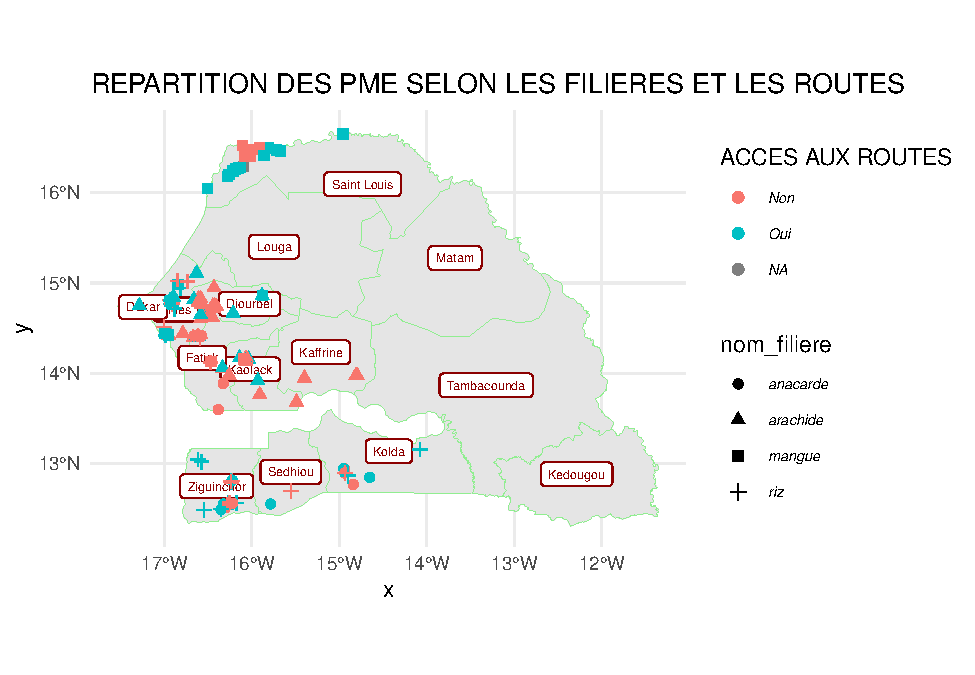
\includegraphics{Projet_R_ISE_1_files/figure-latex/unnamed-chunk-41-1} \end{center}

\begin{Shaded}
\begin{Highlighting}[]
                       \CommentTok{\# de la légende en italique et réduction de la taille}
\end{Highlighting}
\end{Shaded}

\hfill\break

\hypertarget{cruxe9ation-de-la-carte-avec-luxe9tat-des-routes-bitumuxe9es}{%
\subparagraph{Création de la carte avec l'état des routes
bitumées}\label{cruxe9ation-de-la-carte-avec-luxe9tat-des-routes-bitumuxe9es}}

\hfill\break

\begin{Shaded}
\begin{Highlighting}[]
\CommentTok{\# Création de la carte avec l\textquotesingle{}état des routes bitumées}

\NormalTok{projet\_map1}\OtherTok{\textless{}{-}}\NormalTok{projet\_map1 }\SpecialCharTok{\%\textgreater{}\%} \FunctionTok{filter}\NormalTok{(q16}\SpecialCharTok{==}\StringTok{"Oui"}\NormalTok{)}
\FunctionTok{ggplot}\NormalTok{() }\SpecialCharTok{+}
  \FunctionTok{geom\_sf}\NormalTok{(}\AttributeTok{data =}\NormalTok{ OCCreg, }\AttributeTok{color =} \StringTok{"lightgreen"}\NormalTok{) }\SpecialCharTok{+}
  \FunctionTok{geom\_sf\_label}\NormalTok{(}\AttributeTok{data =}\NormalTok{ OCCreg, }\FunctionTok{aes}\NormalTok{(}\AttributeTok{label =}\NormalTok{ adm1\_name), }\AttributeTok{color =} \StringTok{"darkred"}\NormalTok{, }\AttributeTok{size =} \DecValTok{2}\NormalTok{) }\SpecialCharTok{+}
  \FunctionTok{geom\_sf}\NormalTok{(}\AttributeTok{data =}\NormalTok{ projet\_map1, }\FunctionTok{aes}\NormalTok{(}\AttributeTok{fill =}\NormalTok{ nom\_filiere,}\AttributeTok{shape=}\NormalTok{ nom\_filiere, }\AttributeTok{color =}\NormalTok{ q17) , }\AttributeTok{size=}\DecValTok{2}\NormalTok{)}\SpecialCharTok{+}
  \FunctionTok{labs}\NormalTok{(}\AttributeTok{title =} \StringTok{"REPARTITION DES PME SELON LES FILIERES ET L\textquotesingle{}ETAT DES ROUTES"}\NormalTok{,}\AttributeTok{size =} \DecValTok{2}\NormalTok{,}
       \AttributeTok{color =} \StringTok{"ETAT DES ROUTES"}\NormalTok{) }\SpecialCharTok{+}
  \FunctionTok{theme\_minimal}\NormalTok{() }
\end{Highlighting}
\end{Shaded}

\begin{center}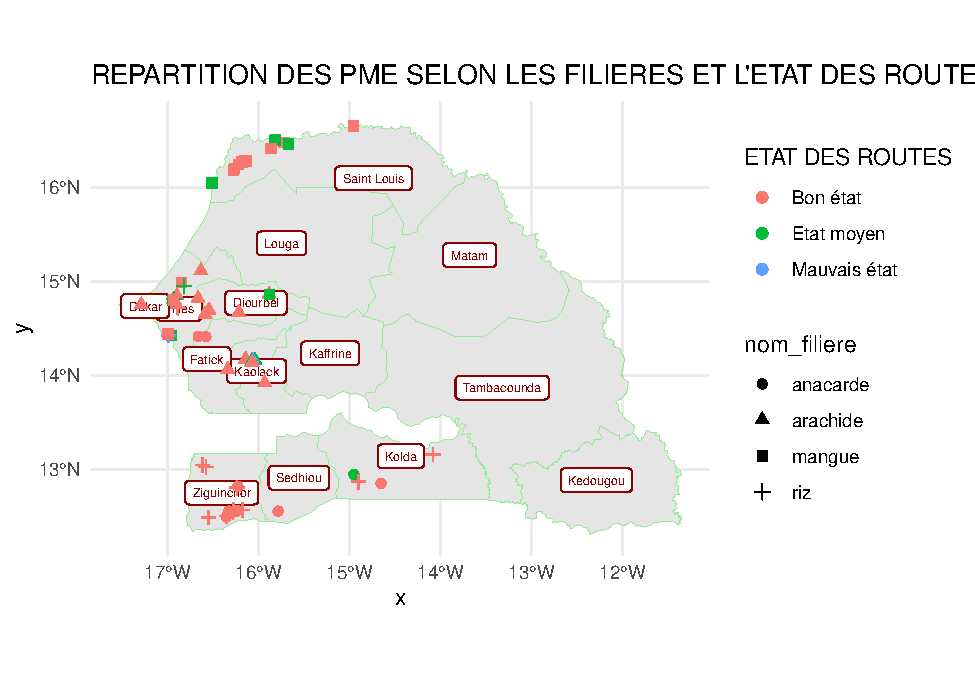
\includegraphics{Projet_R_ISE_1_files/figure-latex/unnamed-chunk-42-1} \end{center}

\hfill\break

\textcolor{blue}{\section{Partie 2.}}

\hfill\break
Le fichier excel Base\_Partie 2.xlsx contient un ensemble de données
artificielles créé dans le cadre de ce projet. La première feuille
contient des micro-données au niveau individuel des répondants à
l'enquête, la deuxième feuille contient des données pour les districts
dans lesquels les répondants de la première feuille ont été interrogés.
La troisième feuille contient des explications sur les variables
incluses dans toutes les feuilles précédentes.\\

\hfill\break

\begin{itemize}
\tightlist
\item
  \textbf{Chargement de données}\\
\end{itemize}

\begin{Shaded}
\begin{Highlighting}[]
\NormalTok{data }\OtherTok{\textless{}{-}} \FunctionTok{read\_excel}\NormalTok{(}\StringTok{"data/Base\_Partie 2.xlsx"}\NormalTok{, }
     \AttributeTok{sheet =} \StringTok{"data"}\NormalTok{)}


\NormalTok{district }\OtherTok{\textless{}{-}} \FunctionTok{read\_excel}\NormalTok{(}\StringTok{"data/Base\_Partie 2.xlsx"}\NormalTok{, }
     \AttributeTok{sheet =} \StringTok{"district"}\NormalTok{)}
\NormalTok{codebook }\OtherTok{\textless{}{-}} \FunctionTok{read\_excel}\NormalTok{(}\StringTok{"data/Base\_Partie 2.xlsx"}\NormalTok{, }
     \AttributeTok{sheet =} \StringTok{"codebook"}\NormalTok{)}
\end{Highlighting}
\end{Shaded}

\hfill\break

\textcolor{blue}{\subsection{Nettoyage et gestion des données.}}

\textcolor{blue}{\subsubsection{Renommation la variable country destination en destination, et définition les valeurs négatives comme manquantes}}

\hfill\break

\begin{Shaded}
\begin{Highlighting}[]
\CommentTok{\# Renommer les variables country\_destination}
\NormalTok{data }\OtherTok{\textless{}{-}}\NormalTok{ data }\SpecialCharTok{\%\textgreater{}\%} 
          \FunctionTok{mutate}\NormalTok{(}\AttributeTok{country\_destination=}\FunctionTok{ifelse}\NormalTok{(country\_destination}\SpecialCharTok{\textgreater{}=}\DecValTok{0}\NormalTok{, }
\NormalTok{                                            country\_destination,}\ConstantTok{NA}\NormalTok{)) }\SpecialCharTok{\%\textgreater{}\%} 
            \FunctionTok{rename}\NormalTok{(}\AttributeTok{destination =}\NormalTok{ country\_destination)  }
\end{Highlighting}
\end{Shaded}

\hfill\break

\textcolor{blue}{\subsubsection{ Créer une nouvelle variable contenant des tranches d'âge de 5 ans en utilisant la variable age.}}

\hfill\break

\begin{Shaded}
\begin{Highlighting}[]
\NormalTok{data}\OtherTok{\textless{}{-}}\NormalTok{ data }\SpecialCharTok{\%\textgreater{}\%}  
         \FunctionTok{mutate}\NormalTok{(}\AttributeTok{age=}\FunctionTok{ifelse}\NormalTok{(age}\SpecialCharTok{==}\DecValTok{999}\NormalTok{, }\ConstantTok{NA}\NormalTok{, age),}
                \AttributeTok{Age\_group=} \FunctionTok{cut}\NormalTok{(age,}\FunctionTok{seq}\NormalTok{(}\DecValTok{14}\NormalTok{, }\AttributeTok{by=}\DecValTok{5}\NormalTok{, }\AttributeTok{length.out=}\DecValTok{7}\NormalTok{)))}

\NormalTok{tab11}\OtherTok{=}\NormalTok{data }\SpecialCharTok{\%\textgreater{}\%} 
\NormalTok{  dplyr}\SpecialCharTok{::}\FunctionTok{select}\NormalTok{(Age\_group) }\SpecialCharTok{\%\textgreater{}\%} 
    \FunctionTok{tbl\_summary}\NormalTok{() }\SpecialCharTok{\%\textgreater{}\%} 
      \FunctionTok{bold\_labels}\NormalTok{()}

\NormalTok{tab11}\SpecialCharTok{\%\textgreater{}\%} \FunctionTok{bold\_labels}\NormalTok{() }\SpecialCharTok{\%\textgreater{}\%} 
  \FunctionTok{italicize\_levels}\NormalTok{()  }\SpecialCharTok{\%\textgreater{}\%} 
  \FunctionTok{modify\_header}\NormalTok{(}\AttributeTok{update =} \FunctionTok{list}\NormalTok{( }
\NormalTok{    label }\SpecialCharTok{\textasciitilde{}} \StringTok{"**VARIABLE**"}\NormalTok{, }\FunctionTok{all\_stat\_cols}\NormalTok{(}
      \AttributeTok{stat\_0 =} \ConstantTok{FALSE}\NormalTok{) }\SpecialCharTok{\textasciitilde{}} \StringTok{"**\{level\}** (n=\{n\}, \{style\_percent(p)\}\%)"}
\NormalTok{  )) }\SpecialCharTok{\%\textgreater{}\%}  \FunctionTok{as\_flex\_table}\NormalTok{() }\SpecialCharTok{\%\textgreater{}\%}
  \FunctionTok{fontsize}\NormalTok{(}\AttributeTok{size =} \DecValTok{8}\NormalTok{) }\SpecialCharTok{\%\textgreater{}\%}
  \FunctionTok{width}\NormalTok{(}\AttributeTok{width =} \FloatTok{1.1}\NormalTok{)}
\end{Highlighting}
\end{Shaded}

\global\setlength{\Oldarrayrulewidth}{\arrayrulewidth}

\global\setlength{\Oldtabcolsep}{\tabcolsep}

\setlength{\tabcolsep}{0pt}

\renewcommand*{\arraystretch}{1.5}



\providecommand{\ascline}[3]{\noalign{\global\arrayrulewidth #1}\arrayrulecolor[HTML]{#2}\cline{#3}}

\begin{longtable}[c]{|p{1.10in}|p{1.10in}}



\ascline{1pt}{000000}{1-2}

\multicolumn{1}{>{\raggedright}m{\dimexpr 1.1in+0\tabcolsep}}{\textcolor[HTML]{000000}{\fontsize{11}{11}\selectfont{\textbf{VARIABLE}}}} & \multicolumn{1}{>{\centering}m{\dimexpr 1.1in+0\tabcolsep}}{\textcolor[HTML]{000000}{\fontsize{11}{11}\selectfont{\textbf{N\ =\ 97}}}\textcolor[HTML]{000000}{\textsuperscript{\fontsize{11}{11}\selectfont{1}}}} \\

\ascline{1pt}{000000}{1-2}\endfirsthead 

\ascline{1pt}{000000}{1-2}

\multicolumn{1}{>{\raggedright}m{\dimexpr 1.1in+0\tabcolsep}}{\textcolor[HTML]{000000}{\fontsize{11}{11}\selectfont{\textbf{VARIABLE}}}} & \multicolumn{1}{>{\centering}m{\dimexpr 1.1in+0\tabcolsep}}{\textcolor[HTML]{000000}{\fontsize{11}{11}\selectfont{\textbf{N\ =\ 97}}}\textcolor[HTML]{000000}{\textsuperscript{\fontsize{11}{11}\selectfont{1}}}} \\

\ascline{1pt}{000000}{1-2}\endhead



\multicolumn{2}{>{\raggedright}m{\dimexpr 2.2in+2\tabcolsep}}{\textcolor[HTML]{000000}{\textsuperscript{\fontsize{11}{11}\selectfont{1}}}\textcolor[HTML]{000000}{\fontsize{11}{11}\selectfont{n\ (\%)}}} \\

\endfoot



\multicolumn{1}{>{\raggedright}p{\dimexpr 1.1in+0\tabcolsep}}{\textcolor[HTML]{000000}{\fontsize{8}{8}\selectfont{\textbf{Age\_group}}}} & \multicolumn{1}{>{\centering}p{\dimexpr 1.1in+0\tabcolsep}}{\textcolor[HTML]{000000}{\fontsize{8}{8}\selectfont{}}} \\





\multicolumn{1}{>{\raggedright}p{\dimexpr 1.1in+0\tabcolsep}}{\textcolor[HTML]{000000}{\fontsize{8}{8}\selectfont{\textit{(14,19]}}}} & \multicolumn{1}{>{\centering}p{\dimexpr 1.1in+0\tabcolsep}}{\textcolor[HTML]{000000}{\fontsize{8}{8}\selectfont{16\ (17\%)}}} \\





\multicolumn{1}{>{\raggedright}p{\dimexpr 1.1in+0\tabcolsep}}{\textcolor[HTML]{000000}{\fontsize{8}{8}\selectfont{\textit{(19,24]}}}} & \multicolumn{1}{>{\centering}p{\dimexpr 1.1in+0\tabcolsep}}{\textcolor[HTML]{000000}{\fontsize{8}{8}\selectfont{34\ (35\%)}}} \\





\multicolumn{1}{>{\raggedright}p{\dimexpr 1.1in+0\tabcolsep}}{\textcolor[HTML]{000000}{\fontsize{8}{8}\selectfont{\textit{(24,29]}}}} & \multicolumn{1}{>{\centering}p{\dimexpr 1.1in+0\tabcolsep}}{\textcolor[HTML]{000000}{\fontsize{8}{8}\selectfont{23\ (24\%)}}} \\





\multicolumn{1}{>{\raggedright}p{\dimexpr 1.1in+0\tabcolsep}}{\textcolor[HTML]{000000}{\fontsize{8}{8}\selectfont{\textit{(29,34]}}}} & \multicolumn{1}{>{\centering}p{\dimexpr 1.1in+0\tabcolsep}}{\textcolor[HTML]{000000}{\fontsize{8}{8}\selectfont{13\ (14\%)}}} \\





\multicolumn{1}{>{\raggedright}p{\dimexpr 1.1in+0\tabcolsep}}{\textcolor[HTML]{000000}{\fontsize{8}{8}\selectfont{\textit{(34,39]}}}} & \multicolumn{1}{>{\centering}p{\dimexpr 1.1in+0\tabcolsep}}{\textcolor[HTML]{000000}{\fontsize{8}{8}\selectfont{6\ (6.3\%)}}} \\





\multicolumn{1}{>{\raggedright}p{\dimexpr 1.1in+0\tabcolsep}}{\textcolor[HTML]{000000}{\fontsize{8}{8}\selectfont{\textit{(39,44]}}}} & \multicolumn{1}{>{\centering}p{\dimexpr 1.1in+0\tabcolsep}}{\textcolor[HTML]{000000}{\fontsize{8}{8}\selectfont{4\ (4.2\%)}}} \\





\multicolumn{1}{>{\raggedright}p{\dimexpr 1.1in+0\tabcolsep}}{\textcolor[HTML]{000000}{\fontsize{8}{8}\selectfont{\textit{Unknown}}}} & \multicolumn{1}{>{\centering}p{\dimexpr 1.1in+0\tabcolsep}}{\textcolor[HTML]{000000}{\fontsize{8}{8}\selectfont{1}}} \\

\ascline{1pt}{000000}{1-2}



\end{longtable}



\arrayrulecolor[HTML]{000000}

\global\setlength{\arrayrulewidth}{\Oldarrayrulewidth}

\global\setlength{\tabcolsep}{\Oldtabcolsep}

\renewcommand*{\arraystretch}{1}

\hfill\break

\textcolor{blue}{\subsubsection{Créer une nouvelle variable contenant le nombre d'entretiens réalisés par chaque agent recenseur.}}

\hfill\break

\begin{Shaded}
\begin{Highlighting}[]
\NormalTok{data}\OtherTok{\textless{}{-}}\NormalTok{data }\SpecialCharTok{\%\textgreater{}\%} 
          \FunctionTok{mutate}\NormalTok{(}\AttributeTok{enumerator=}\FunctionTok{as.factor}\NormalTok{(enumerator))}
\CommentTok{\# Création du tableau}
\NormalTok{tab12}\OtherTok{=}\NormalTok{data }\SpecialCharTok{\%\textgreater{}\%} 
\NormalTok{    dplyr}\SpecialCharTok{::}\FunctionTok{select}\NormalTok{(enumerator) }\SpecialCharTok{\%\textgreater{}\%} 
            \FunctionTok{rename}\NormalTok{(}\StringTok{"Numero de l\textquotesingle{}agent recenseur"}\OtherTok{=}\NormalTok{enumerator) }\SpecialCharTok{\%\textgreater{}\%} 
                \FunctionTok{tbl\_summary}\NormalTok{(}\AttributeTok{sort =} \FunctionTok{list}\NormalTok{(}\FunctionTok{everything}\NormalTok{() }\SpecialCharTok{\textasciitilde{}} \StringTok{"frequency"}\NormalTok{)) }\SpecialCharTok{\%\textgreater{}\%} \FunctionTok{bold\_labels}\NormalTok{()}

\NormalTok{tab12\_kable }\OtherTok{\textless{}{-}} \FunctionTok{as\_kable}\NormalTok{(tab12) }\SpecialCharTok{\%\textgreater{}\%}  
   \FunctionTok{kable\_paper}\NormalTok{(}\AttributeTok{full\_width =} \ConstantTok{TRUE}\NormalTok{)}\SpecialCharTok{\%\textgreater{}\%}
  \FunctionTok{row\_spec}\NormalTok{(}\DecValTok{0}\SpecialCharTok{:}\DecValTok{1}\NormalTok{, }\AttributeTok{background =} \StringTok{"green"}\NormalTok{, }\AttributeTok{color =} \StringTok{"black"}\NormalTok{) }\SpecialCharTok{\%\textgreater{}\%}
  \FunctionTok{row\_spec}\NormalTok{(}\DecValTok{2}\SpecialCharTok{:}\DecValTok{3}\NormalTok{, }\AttributeTok{background =} \StringTok{"\#90EE90"}\NormalTok{, }\AttributeTok{color =} \StringTok{"black"}\NormalTok{) }\SpecialCharTok{\%\textgreater{}\%} 
  \FunctionTok{row\_spec}\NormalTok{(}\DecValTok{4}\SpecialCharTok{:}\DecValTok{12}\NormalTok{, }\AttributeTok{background =} \StringTok{"\#FFFFE0"}\NormalTok{, }\AttributeTok{color =} \StringTok{"black"}\NormalTok{)}

\CommentTok{\# Afficher la table avec les deux premières lignes colorées en vert}
\NormalTok{tab12\_kable}
\end{Highlighting}
\end{Shaded}

\begin{tabu} to \linewidth {>{\raggedright}X>{\centering}X}
\hline
\cellcolor{green}{\textcolor{black}{**Characteristic**}} & \cellcolor{green}{\textcolor{black}{**N = 97**}}\\
\hline
\cellcolor{green}{\textcolor{black}{\_\_Numero de l'agent recenseur\_\_}} & \cellcolor{green}{\textcolor{black}{}}\\
\hline
\cellcolor[HTML]{90EE90}{\textcolor{black}{4}} & \cellcolor[HTML]{90EE90}{\textcolor{black}{9 (9.3\%)}}\\
\hline
\cellcolor[HTML]{90EE90}{\textcolor{black}{20}} & \cellcolor[HTML]{90EE90}{\textcolor{black}{9 (9.3\%)}}\\
\hline
\cellcolor[HTML]{FFFFE0}{\textcolor{black}{13}} & \cellcolor[HTML]{FFFFE0}{\textcolor{black}{8 (8.2\%)}}\\
\hline
\cellcolor[HTML]{FFFFE0}{\textcolor{black}{7}} & \cellcolor[HTML]{FFFFE0}{\textcolor{black}{7 (7.2\%)}}\\
\hline
\cellcolor[HTML]{FFFFE0}{\textcolor{black}{11}} & \cellcolor[HTML]{FFFFE0}{\textcolor{black}{7 (7.2\%)}}\\
\hline
\cellcolor[HTML]{FFFFE0}{\textcolor{black}{5}} & \cellcolor[HTML]{FFFFE0}{\textcolor{black}{6 (6.2\%)}}\\
\hline
\cellcolor[HTML]{FFFFE0}{\textcolor{black}{8}} & \cellcolor[HTML]{FFFFE0}{\textcolor{black}{6 (6.2\%)}}\\
\hline
\cellcolor[HTML]{FFFFE0}{\textcolor{black}{9}} & \cellcolor[HTML]{FFFFE0}{\textcolor{black}{6 (6.2\%)}}\\
\hline
\cellcolor[HTML]{FFFFE0}{\textcolor{black}{14}} & \cellcolor[HTML]{FFFFE0}{\textcolor{black}{6 (6.2\%)}}\\
\hline
\cellcolor[HTML]{FFFFE0}{\textcolor{black}{17}} & \cellcolor[HTML]{FFFFE0}{\textcolor{black}{6 (6.2\%)}}\\
\hline
\cellcolor[HTML]{FFFFE0}{\textcolor{black}{18}} & \cellcolor[HTML]{FFFFE0}{\textcolor{black}{6 (6.2\%)}}\\
\hline
1 & 5 (5.2\%)\\
\hline
6 & 5 (5.2\%)\\
\hline
10 & 5 (5.2\%)\\
\hline
12 & 5 (5.2\%)\\
\hline
15 & 1 (1.0\%)\\
\hline
\end{tabu}

\hfill\break

il apparait que se sont \textbf{les ressenceurs 4 et 20} qui ont le plus
grand nombre de recensement soit \textbf{9 reccensements}\\

\hypertarget{cruxe9er-une-nouvelle-variable-qui-affecte-aluxe9atoirement-chaque-ruxe9pondant-uxe0-un-groupe-de-traitement-1-ou-de-controle-0.}{%
\paragraph{Créer une nouvelle variable qui affecte aléatoirement chaque
répondant à un groupe de traitement (1) ou de controle
(0).}\label{cruxe9er-une-nouvelle-variable-qui-affecte-aluxe9atoirement-chaque-ruxe9pondant-uxe0-un-groupe-de-traitement-1-ou-de-controle-0.}}

\hfill\break

\begin{Shaded}
\begin{Highlighting}[]
\NormalTok{data}\OtherTok{\textless{}{-}}\NormalTok{data }\SpecialCharTok{\%\textgreater{}\%} 
          \FunctionTok{mutate}\NormalTok{(}\AttributeTok{traitement=}\FunctionTok{sample}\NormalTok{(}\FunctionTok{c}\NormalTok{(}\DecValTok{0}\NormalTok{,}\DecValTok{1}\NormalTok{), }\DecValTok{97}\NormalTok{, }\AttributeTok{replace =} \ConstantTok{TRUE}\NormalTok{))}
\end{Highlighting}
\end{Shaded}

\hfill\break

\hypertarget{fusionner-la-taille-de-la-population-de-chaque-district-feuille-2-avec-lensemble-de-donnuxe9es-feuille-1-afin-que-toutes-les-personnes-interroguxe9es-aient-une-valeur-correspondante-repruxe9sentant-la-taille-de-la-population-du-district-dans-lequel-elles-vivent.}{%
\paragraph{\texorpdfstring{Fusionner la taille de la population de
chaque district (feuille 2) avec l'ensemble de données (feuille 1) afin
que toutes les personnes interrogées aient une valeur correspondante
représentant la taille de la population du district dans lequel elles
vivent.\\
}{Fusionner la taille de la population de chaque district (feuille 2) avec l'ensemble de données (feuille 1) afin que toutes les personnes interrogées aient une valeur correspondante représentant la taille de la population du district dans lequel elles vivent. }}\label{fusionner-la-taille-de-la-population-de-chaque-district-feuille-2-avec-lensemble-de-donnuxe9es-feuille-1-afin-que-toutes-les-personnes-interroguxe9es-aient-une-valeur-correspondante-repruxe9sentant-la-taille-de-la-population-du-district-dans-lequel-elles-vivent.}}

\begin{Shaded}
\begin{Highlighting}[]
\CommentTok{\# jointure a gauche}
\NormalTok{d}\OtherTok{\textless{}{-}} \FunctionTok{data\_merge}\NormalTok{(data, district, }\AttributeTok{join =} \StringTok{"left"}\NormalTok{, }\AttributeTok{id =}\NormalTok{ district)}
\end{Highlighting}
\end{Shaded}

\textcolor{blue}{\subsubsection{ Calculer la durée de l'entretien et indiquer la durée moyenne de l'entretien par enquêteur.}}

\hfill\break

\begin{Shaded}
\begin{Highlighting}[]
\CommentTok{\#calcul de la duree}
\NormalTok{d}\OtherTok{\textless{}{-}}\NormalTok{d }\SpecialCharTok{\%\textgreater{}\%} 
     \FunctionTok{mutate}\NormalTok{(}\AttributeTok{duree=}\NormalTok{endtime}\SpecialCharTok{{-}}\NormalTok{starttime)}

\CommentTok{\#calcul de la duree moyenne par enqueteur}

\NormalTok{d }\SpecialCharTok{\%\textgreater{}\%}
  \FunctionTok{group\_by}\NormalTok{(enumerator) }\SpecialCharTok{\%\textgreater{}\%} 
     \FunctionTok{rename}\NormalTok{(}\StringTok{"Numero de l\textquotesingle{}agent recenseur"}\OtherTok{=}\NormalTok{enumerator) }\SpecialCharTok{\%\textgreater{}\%} 
        \FunctionTok{summarise}\NormalTok{(}\AttributeTok{dureemoy =} \FunctionTok{mean}\NormalTok{(duree), }\AttributeTok{nbre\_enquete =} \FunctionTok{n}\NormalTok{()) }\SpecialCharTok{\%\textgreater{}\%} 
          \FunctionTok{kbl}\NormalTok{() }\SpecialCharTok{\%\textgreater{}\%}
          \FunctionTok{kable\_paper}\NormalTok{(}\AttributeTok{full\_width =} \ConstantTok{TRUE}\NormalTok{) }\SpecialCharTok{\%\textgreater{}\%}
          \FunctionTok{row\_spec}\NormalTok{(}\DecValTok{0}\SpecialCharTok{:}\DecValTok{1}\NormalTok{, }\AttributeTok{background =} \StringTok{"green"}\NormalTok{,}\AttributeTok{color=}\StringTok{"black"}\NormalTok{) }\SpecialCharTok{\%\textgreater{}\%} 
          \FunctionTok{row\_spec}\NormalTok{(}\DecValTok{1}\SpecialCharTok{:}\DecValTok{16}\NormalTok{, }\AttributeTok{background =} \StringTok{"lightgray"}\NormalTok{,}\AttributeTok{color=}\StringTok{"black"}\NormalTok{)}
\end{Highlighting}
\end{Shaded}

\begin{tabu} to \linewidth {>{\raggedright}X>{\raggedright}X>{\raggedleft}X}
\hline
\cellcolor{green}{\textcolor{black}{Numero de l'agent recenseur}} & \cellcolor{green}{\textcolor{black}{dureemoy}} & \cellcolor{green}{\textcolor{black}{nbre\_enquete}}\\
\hline
\cellcolor{lightgray}{\textcolor{black}{1}} & \cellcolor{lightgray}{\textcolor{black}{68.14667 mins}} & \cellcolor{lightgray}{\textcolor{black}{5}}\\
\hline
\cellcolor{lightgray}{\textcolor{black}{4}} & \cellcolor{lightgray}{\textcolor{black}{36.48333 mins}} & \cellcolor{lightgray}{\textcolor{black}{9}}\\
\hline
\cellcolor{lightgray}{\textcolor{black}{5}} & \cellcolor{lightgray}{\textcolor{black}{33.55833 mins}} & \cellcolor{lightgray}{\textcolor{black}{6}}\\
\hline
\cellcolor{lightgray}{\textcolor{black}{6}} & \cellcolor{lightgray}{\textcolor{black}{25.84667 mins}} & \cellcolor{lightgray}{\textcolor{black}{5}}\\
\hline
\cellcolor{lightgray}{\textcolor{black}{7}} & \cellcolor{lightgray}{\textcolor{black}{37.16429 mins}} & \cellcolor{lightgray}{\textcolor{black}{7}}\\
\hline
\cellcolor{lightgray}{\textcolor{black}{8}} & \cellcolor{lightgray}{\textcolor{black}{40.13056 mins}} & \cellcolor{lightgray}{\textcolor{black}{6}}\\
\hline
\cellcolor{lightgray}{\textcolor{black}{9}} & \cellcolor{lightgray}{\textcolor{black}{114.76667 mins}} & \cellcolor{lightgray}{\textcolor{black}{6}}\\
\hline
\cellcolor{lightgray}{\textcolor{black}{10}} & \cellcolor{lightgray}{\textcolor{black}{55.27667 mins}} & \cellcolor{lightgray}{\textcolor{black}{5}}\\
\hline
\cellcolor{lightgray}{\textcolor{black}{11}} & \cellcolor{lightgray}{\textcolor{black}{33.48333 mins}} & \cellcolor{lightgray}{\textcolor{black}{7}}\\
\hline
\cellcolor{lightgray}{\textcolor{black}{12}} & \cellcolor{lightgray}{\textcolor{black}{48.16667 mins}} & \cellcolor{lightgray}{\textcolor{black}{5}}\\
\hline
\cellcolor{lightgray}{\textcolor{black}{13}} & \cellcolor{lightgray}{\textcolor{black}{31.59583 mins}} & \cellcolor{lightgray}{\textcolor{black}{8}}\\
\hline
\cellcolor{lightgray}{\textcolor{black}{14}} & \cellcolor{lightgray}{\textcolor{black}{25.56111 mins}} & \cellcolor{lightgray}{\textcolor{black}{6}}\\
\hline
\cellcolor{lightgray}{\textcolor{black}{15}} & \cellcolor{lightgray}{\textcolor{black}{28.65000 mins}} & \cellcolor{lightgray}{\textcolor{black}{1}}\\
\hline
\cellcolor{lightgray}{\textcolor{black}{17}} & \cellcolor{lightgray}{\textcolor{black}{29.28611 mins}} & \cellcolor{lightgray}{\textcolor{black}{6}}\\
\hline
\cellcolor{lightgray}{\textcolor{black}{18}} & \cellcolor{lightgray}{\textcolor{black}{36.85833 mins}} & \cellcolor{lightgray}{\textcolor{black}{6}}\\
\hline
\cellcolor{lightgray}{\textcolor{black}{20}} & \cellcolor{lightgray}{\textcolor{black}{28.76852 mins}} & \cellcolor{lightgray}{\textcolor{black}{9}}\\
\hline
\end{tabu}

\hfill\break

\hypertarget{renommez-toutes-les-variables-de-lensemble-de-donnuxe9es-en-ajoutant-le-pruxe9fixe-endline_-uxe0-laide-dune-boucle.}{%
\paragraph{Renommez toutes les variables de l'ensemble de données en
ajoutant le préfixe ``endline\_'' à l'aide d'une
boucle.\}\}}\label{renommez-toutes-les-variables-de-lensemble-de-donnuxe9es-en-ajoutant-le-pruxe9fixe-endline_-uxe0-laide-dune-boucle.}}

\hfill\break

\begin{Shaded}
\begin{Highlighting}[]
\NormalTok{d1}\OtherTok{\textless{}{-}}\NormalTok{d}
\CommentTok{\#nom des colonnes}
\NormalTok{colon}\OtherTok{\textless{}{-}}\FunctionTok{colnames}\NormalTok{(d)}
 
\CommentTok{\# Nouveaux noms de variables avec le préfixe "endline\_"}
\NormalTok{new\_col }\OtherTok{\textless{}{-}} \FunctionTok{paste0}\NormalTok{(}\StringTok{"endline\_"}\NormalTok{, colon)}

\CommentTok{\# Renommage des variables à l\textquotesingle{}aide d\textquotesingle{}une boucle}
\ControlFlowTok{for}\NormalTok{ (i }\ControlFlowTok{in} \FunctionTok{seq\_along}\NormalTok{(colon)) \{}
  \FunctionTok{colnames}\NormalTok{(d)[i] }\OtherTok{\textless{}{-}}\NormalTok{ new\_col[i]}
\NormalTok{\}}
\end{Highlighting}
\end{Shaded}

\hfill\break

\hypertarget{renommez-toutes-les-variables-de-lensemble-de-donnuxe9es-en-ajoutant-le-pruxe9fixe-endline_-avec-lapply}{%
\paragraph{Renommez toutes les variables de l'ensemble de données en
ajoutant le préfixe ``endline\_'' avec
lapply}\label{renommez-toutes-les-variables-de-lensemble-de-donnuxe9es-en-ajoutant-le-pruxe9fixe-endline_-avec-lapply}}

\hfill\break

\begin{Shaded}
\begin{Highlighting}[]
\NormalTok{noms\_nouveaux }\OtherTok{\textless{}{-}} \FunctionTok{lapply}\NormalTok{(}\FunctionTok{names}\NormalTok{(d1), }\ControlFlowTok{function}\NormalTok{(col) }\FunctionTok{paste0}\NormalTok{(}\StringTok{"endline\_"}\NormalTok{, col))}
\FunctionTok{names}\NormalTok{(d1) }\OtherTok{\textless{}{-}} \FunctionTok{unlist}\NormalTok{(noms\_nouveaux)}
\NormalTok{d1 }\SpecialCharTok{\%\textgreater{}\%}
\FunctionTok{names}\NormalTok{()}
\end{Highlighting}
\end{Shaded}

\begin{verbatim}
##  [1] "endline_id"           "endline_starttime"    "endline_endtime"     
##  [4] "endline_enumerator"   "endline_district"     "endline_age"         
##  [7] "endline_sex"          "endline_children_num" "endline_intention"   
## [10] "endline_destination"  "endline_Age_group"    "endline_traitement"  
## [13] "endline_population"   "endline_duree"
\end{verbatim}

\hfill\break

\textcolor{blue}{\subsection{Analyse et visualisation des données.}}

\textcolor{blue}{\subsubsection{Créez un tableau récapitulatif contenant l'âge moyen et le nombre moyen d'enfants par district.}}

\hfill\break

\begin{Shaded}
\begin{Highlighting}[]
\NormalTok{data }\SpecialCharTok{\%\textgreater{}\%}
  \FunctionTok{group\_by}\NormalTok{(district) }\SpecialCharTok{\%\textgreater{}\%}
     \FunctionTok{summarise}\NormalTok{(}\AttributeTok{age\_moyen =} \FunctionTok{round}\NormalTok{(}\FunctionTok{mean}\NormalTok{(age, }\AttributeTok{na.rm=}\ConstantTok{TRUE}\NormalTok{),}\DecValTok{2}\NormalTok{), }
               \AttributeTok{enfants\_moyen =} \FunctionTok{round}\NormalTok{(}\FunctionTok{mean}\NormalTok{(children\_num, }\AttributeTok{na.rm=}\ConstantTok{TRUE}\NormalTok{),}\DecValTok{2}\NormalTok{))  }\SpecialCharTok{\%\textgreater{}\%} 
        \FunctionTok{kbl}\NormalTok{() }\SpecialCharTok{\%\textgreater{}\%}
          \FunctionTok{kable\_paper}\NormalTok{(}\AttributeTok{full\_width =} \ConstantTok{TRUE}\NormalTok{) }\SpecialCharTok{\%\textgreater{}\%}
          \FunctionTok{row\_spec}\NormalTok{(}\DecValTok{0}\SpecialCharTok{:}\DecValTok{1}\NormalTok{, }\AttributeTok{background =} \StringTok{"green"}\NormalTok{,}\AttributeTok{color=}\StringTok{"black"}\NormalTok{) }\SpecialCharTok{\%\textgreater{}\%} 
          \FunctionTok{row\_spec}\NormalTok{(}\DecValTok{1}\SpecialCharTok{:}\DecValTok{8}\NormalTok{, }\AttributeTok{background =} \StringTok{"lightgray"}\NormalTok{,}\AttributeTok{color=}\StringTok{"black"}\NormalTok{)}
\end{Highlighting}
\end{Shaded}

\begin{tabu} to \linewidth {>{\raggedleft}X>{\raggedleft}X>{\raggedleft}X}
\hline
\cellcolor{green}{\textcolor{black}{district}} & \cellcolor{green}{\textcolor{black}{age\_moyen}} & \cellcolor{green}{\textcolor{black}{enfants\_moyen}}\\
\hline
\cellcolor{lightgray}{\textcolor{black}{1}} & \cellcolor{lightgray}{\textcolor{black}{29.62}} & \cellcolor{lightgray}{\textcolor{black}{1.50}}\\
\hline
\cellcolor{lightgray}{\textcolor{black}{2}} & \cellcolor{lightgray}{\textcolor{black}{26.62}} & \cellcolor{lightgray}{\textcolor{black}{0.85}}\\
\hline
\cellcolor{lightgray}{\textcolor{black}{3}} & \cellcolor{lightgray}{\textcolor{black}{26.12}} & \cellcolor{lightgray}{\textcolor{black}{0.00}}\\
\hline
\cellcolor{lightgray}{\textcolor{black}{4}} & \cellcolor{lightgray}{\textcolor{black}{26.00}} & \cellcolor{lightgray}{\textcolor{black}{0.00}}\\
\hline
\cellcolor{lightgray}{\textcolor{black}{5}} & \cellcolor{lightgray}{\textcolor{black}{24.33}} & \cellcolor{lightgray}{\textcolor{black}{0.50}}\\
\hline
\cellcolor{lightgray}{\textcolor{black}{6}} & \cellcolor{lightgray}{\textcolor{black}{23.15}} & \cellcolor{lightgray}{\textcolor{black}{0.12}}\\
\hline
\cellcolor{lightgray}{\textcolor{black}{7}} & \cellcolor{lightgray}{\textcolor{black}{28.00}} & \cellcolor{lightgray}{\textcolor{black}{0.17}}\\
\hline
\cellcolor{lightgray}{\textcolor{black}{8}} & \cellcolor{lightgray}{\textcolor{black}{24.64}} & \cellcolor{lightgray}{\textcolor{black}{1.27}}\\
\hline
\end{tabu}

\hfill\break

\textcolor{blue}{\subsection{Les tests}}

\begin{itemize}
\tightlist
\item
  Testez si la différence d'âge entre les sexes est statistiquement
  significative au niveau de 5 \%.\\
  Il est necessaire de faire un test d'annova afin de savoir comment
  definir notre test de significtivité
\end{itemize}

\textcolor{blue}{\subsubsection{Annova}}

\hfill\break

\begin{Shaded}
\begin{Highlighting}[]
\CommentTok{\#test d\textquotesingle{}égalité des variance}
\NormalTok{mod }\OtherTok{\textless{}{-}} \FunctionTok{anova}\NormalTok{(}\FunctionTok{lm}\NormalTok{(age }\SpecialCharTok{\textasciitilde{}}\NormalTok{ sex, data))}
\FunctionTok{bind\_rows}\NormalTok{(}
\NormalTok{  broom}\SpecialCharTok{::}\FunctionTok{tidy}\NormalTok{(mod) }
\NormalTok{)}\SpecialCharTok{\%\textgreater{}\%}
  \FunctionTok{kbl}\NormalTok{() }\SpecialCharTok{\%\textgreater{}\%}
          \FunctionTok{kable\_paper}\NormalTok{(}\AttributeTok{full\_width =} \ConstantTok{TRUE}\NormalTok{) }\SpecialCharTok{\%\textgreater{}\%}
          \FunctionTok{row\_spec}\NormalTok{(}\DecValTok{0}\SpecialCharTok{:}\DecValTok{1}\NormalTok{, }\AttributeTok{background =} \StringTok{"green"}\NormalTok{,}\AttributeTok{color=}\StringTok{"black"}\NormalTok{) }\SpecialCharTok{\%\textgreater{}\%} 
          \FunctionTok{row\_spec}\NormalTok{(}\DecValTok{1}\SpecialCharTok{:}\DecValTok{2}\NormalTok{, }\AttributeTok{background =} \StringTok{"lightgray"}\NormalTok{,}\AttributeTok{color=}\StringTok{"black"}\NormalTok{)}
\end{Highlighting}
\end{Shaded}

\begin{tabu} to \linewidth {>{\raggedright}X>{\raggedleft}X>{\raggedleft}X>{\raggedleft}X>{\raggedleft}X>{\raggedleft}X}
\hline
\cellcolor{green}{\textcolor{black}{term}} & \cellcolor{green}{\textcolor{black}{df}} & \cellcolor{green}{\textcolor{black}{sumsq}} & \cellcolor{green}{\textcolor{black}{meansq}} & \cellcolor{green}{\textcolor{black}{statistic}} & \cellcolor{green}{\textcolor{black}{p.value}}\\
\hline
\cellcolor{lightgray}{\textcolor{black}{sex}} & \cellcolor{lightgray}{\textcolor{black}{1}} & \cellcolor{lightgray}{\textcolor{black}{142.5012}} & \cellcolor{lightgray}{\textcolor{black}{142.50121}} & \cellcolor{lightgray}{\textcolor{black}{3.55781}} & \cellcolor{lightgray}{\textcolor{black}{0.062353}}\\
\hline
\cellcolor{lightgray}{\textcolor{black}{Residuals}} & \cellcolor{lightgray}{\textcolor{black}{94}} & \cellcolor{lightgray}{\textcolor{black}{3764.9884}} & \cellcolor{lightgray}{\textcolor{black}{40.05307}} & \cellcolor{lightgray}{\textcolor{black}{NA}} & \cellcolor{lightgray}{\textcolor{black}{NA}}\\
\hline
\end{tabu}

\hfill\break
donc les varainces sont égales

\textcolor{blue}{\subsubsection{Test de student}}

\hfill\break

\begin{Shaded}
\begin{Highlighting}[]
\CommentTok{\#test de student}
\NormalTok{mod}\OtherTok{\textless{}{-}}\FunctionTok{t.test}\NormalTok{(age }\SpecialCharTok{\textasciitilde{}}\NormalTok{ sex, data, }\AttributeTok{var.equal =} \ConstantTok{TRUE}\NormalTok{)}
\FunctionTok{bind\_rows}\NormalTok{(}
\NormalTok{  broom}\SpecialCharTok{::}\FunctionTok{tidy}\NormalTok{(mod) }
\NormalTok{)}\SpecialCharTok{\%\textgreater{}\%}
  \FunctionTok{kbl}\NormalTok{() }\SpecialCharTok{\%\textgreater{}\%}
          \FunctionTok{kable\_paper}\NormalTok{(}\AttributeTok{full\_width =} \ConstantTok{TRUE}\NormalTok{) }\SpecialCharTok{\%\textgreater{}\%}
          \FunctionTok{row\_spec}\NormalTok{(}\DecValTok{0}\SpecialCharTok{:}\DecValTok{1}\NormalTok{, }\AttributeTok{background =} \StringTok{"green"}\NormalTok{,}\AttributeTok{color=}\StringTok{"black"}\NormalTok{) }\SpecialCharTok{\%\textgreater{}\%} 
          \FunctionTok{row\_spec}\NormalTok{(}\DecValTok{1}\SpecialCharTok{:}\DecValTok{1}\NormalTok{, }\AttributeTok{background =} \StringTok{"lightgray"}\NormalTok{,}\AttributeTok{color=}\StringTok{"black"}\NormalTok{)}
\end{Highlighting}
\end{Shaded}

\begin{tabu} to \linewidth {>{\raggedleft}X>{\raggedleft}X>{\raggedleft}X>{\raggedleft}X>{\raggedleft}X>{\raggedleft}X>{\raggedleft}X>{\raggedleft}X>{\raggedright}X>{\raggedright}X}
\hline
\cellcolor{green}{\textcolor{black}{estimate}} & \cellcolor{green}{\textcolor{black}{estimate1}} & \cellcolor{green}{\textcolor{black}{estimate2}} & \cellcolor{green}{\textcolor{black}{statistic}} & \cellcolor{green}{\textcolor{black}{p.value}} & \cellcolor{green}{\textcolor{black}{parameter}} & \cellcolor{green}{\textcolor{black}{conf.low}} & \cellcolor{green}{\textcolor{black}{conf.high}} & \cellcolor{green}{\textcolor{black}{method}} & \cellcolor{green}{\textcolor{black}{alternative}}\\
\hline
\cellcolor{lightgray}{\textcolor{black}{3.988372}} & \cellcolor{lightgray}{\textcolor{black}{25.98837}} & \cellcolor{lightgray}{\textcolor{black}{22}} & \cellcolor{lightgray}{\textcolor{black}{1.886216}} & \cellcolor{lightgray}{\textcolor{black}{0.062353}} & \cellcolor{lightgray}{\textcolor{black}{94}} & \cellcolor{lightgray}{\textcolor{black}{-0.2099843}} & \cellcolor{lightgray}{\textcolor{black}{8.186728}} & \cellcolor{lightgray}{\textcolor{black}{Two Sample t-test}} & \cellcolor{lightgray}{\textcolor{black}{two.sided}}\\
\hline
\end{tabu}

\hfill\break

\textcolor{blue}{\subsubsection{Créer un nuage de points de l'âge en fonction du nombre d'enfants}}

\hfill\break

\begin{Shaded}
\begin{Highlighting}[]
\FunctionTok{ggplot}\NormalTok{(data, }\FunctionTok{aes}\NormalTok{(}\AttributeTok{x =}\NormalTok{ age, }\AttributeTok{y =}\NormalTok{ children\_num)) }\SpecialCharTok{+}
  \FunctionTok{geom\_point}\NormalTok{() }\SpecialCharTok{+}
  \FunctionTok{labs}\NormalTok{(}\AttributeTok{x =} \StringTok{"Âge"}\NormalTok{, }\AttributeTok{y =} \StringTok{"Nombre d\textquotesingle{}enfants"}\NormalTok{)}
\end{Highlighting}
\end{Shaded}

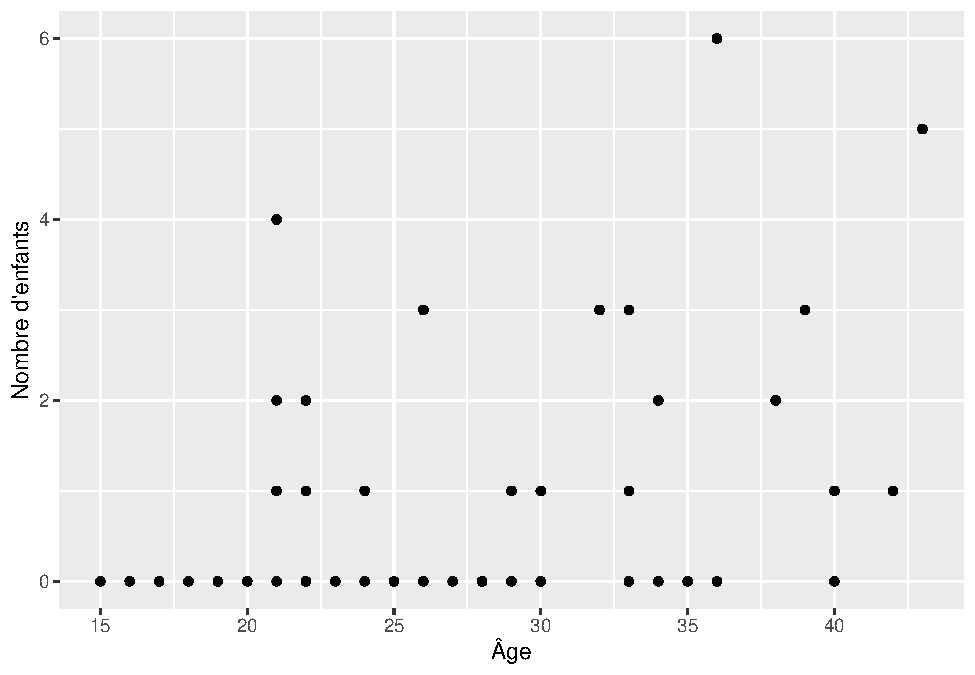
\includegraphics{Projet_R_ISE_1_files/figure-latex/unnamed-chunk-55-1.pdf}\\

\textcolor{blue}{\subsubsection{Effet appartenance et intention}}

\hfill\break

\hypertarget{la-variable-intention-indique-si-les-migrants-potentiels-ont-lintention-de-migrer-sur-une-uxe9chelle-de-1-uxe0-7.-estimez-leffet-de-lappartenance-au-groupe-de-traitement-sur-lintention-de-migrer.}{%
\paragraph{La variable ``intention'' indique si les migrants potentiels
ont l'intention de migrer sur une échelle de 1 à 7. Estimez l'effet de
l'appartenance au groupe de traitement sur l'intention de
migrer.}\label{la-variable-intention-indique-si-les-migrants-potentiels-ont-lintention-de-migrer-sur-une-uxe9chelle-de-1-uxe0-7.-estimez-leffet-de-lappartenance-au-groupe-de-traitement-sur-lintention-de-migrer.}}

\hfill\break

\begin{Shaded}
\begin{Highlighting}[]
\NormalTok{modele\_traitement}\OtherTok{\textless{}{-}}\FunctionTok{lm}\NormalTok{(intention }\SpecialCharTok{\textasciitilde{}}\NormalTok{ traitement}\DecValTok{{-}1}\NormalTok{, data)}
\NormalTok{effet\_traitement }\OtherTok{\textless{}{-}} \FunctionTok{coef}\NormalTok{(modele\_traitement)[}\StringTok{"traitement"}\NormalTok{]}

\NormalTok{mod }\OtherTok{\textless{}{-}} \FunctionTok{summary}\NormalTok{(modele\_traitement)}
\FunctionTok{bind\_rows}\NormalTok{(}
\NormalTok{  broom}\SpecialCharTok{::}\FunctionTok{tidy}\NormalTok{(mod) }
\NormalTok{)}\SpecialCharTok{\%\textgreater{}\%}
  \FunctionTok{kbl}\NormalTok{() }\SpecialCharTok{\%\textgreater{}\%}
          \FunctionTok{kable\_paper}\NormalTok{(}\AttributeTok{full\_width =} \ConstantTok{TRUE}\NormalTok{) }\SpecialCharTok{\%\textgreater{}\%}
          \FunctionTok{row\_spec}\NormalTok{(}\DecValTok{0}\SpecialCharTok{:}\DecValTok{1}\NormalTok{, }\AttributeTok{background =} \StringTok{"green"}\NormalTok{,}\AttributeTok{color=}\StringTok{"black"}\NormalTok{) }\SpecialCharTok{\%\textgreater{}\%} 
          \FunctionTok{row\_spec}\NormalTok{(}\DecValTok{1}\SpecialCharTok{:}\DecValTok{1}\NormalTok{, }\AttributeTok{background =} \StringTok{"lightgray"}\NormalTok{,}\AttributeTok{color=}\StringTok{"black"}\NormalTok{)}
\end{Highlighting}
\end{Shaded}

\begin{tabu} to \linewidth {>{\raggedright}X>{\raggedleft}X>{\raggedleft}X>{\raggedleft}X>{\raggedleft}X}
\hline
\cellcolor{green}{\textcolor{black}{term}} & \cellcolor{green}{\textcolor{black}{estimate}} & \cellcolor{green}{\textcolor{black}{std.error}} & \cellcolor{green}{\textcolor{black}{statistic}} & \cellcolor{green}{\textcolor{black}{p.value}}\\
\hline
\cellcolor{lightgray}{\textcolor{black}{traitement}} & \cellcolor{lightgray}{\textcolor{black}{2}} & \cellcolor{lightgray}{\textcolor{black}{0.2926911}} & \cellcolor{lightgray}{\textcolor{black}{6.833142}} & \cellcolor{lightgray}{\textcolor{black}{0}}\\
\hline
\end{tabu}

\hfill\break

\textcolor{blue}{\subsubsection{Presentation des modèles}}

\hfill\break
Crée un tableau de régression avec 3 modèles. La variable de résultat
est toujours ``intention''. Modèle A : Modèle vide - Effet du traitement
sur les intentions. Modèle B : Effet du traitement sur les intentions en
tenant compte de l'âge et du sexe. Modèle C : Identique au modèle B mais
en contrôlant le district. Les résultats des trois modèles doivent être
affichés dans un seul tableau.

\hfill\break

\begin{Shaded}
\begin{Highlighting}[]
\NormalTok{modele\_a }\OtherTok{\textless{}{-}} \FunctionTok{lm}\NormalTok{(intention }\SpecialCharTok{\textasciitilde{}}\NormalTok{ traitement}\DecValTok{{-}1}\NormalTok{, data)}
\NormalTok{modele\_b }\OtherTok{\textless{}{-}} \FunctionTok{lm}\NormalTok{(intention }\SpecialCharTok{\textasciitilde{}}\NormalTok{ traitement }\SpecialCharTok{{-}}\DecValTok{1}\SpecialCharTok{+}\NormalTok{ age }\SpecialCharTok{+}\NormalTok{ sex, data )}
\NormalTok{modele\_c }\OtherTok{\textless{}{-}} \FunctionTok{lm}\NormalTok{(intention }\SpecialCharTok{\textasciitilde{}}\NormalTok{ traitement }\SpecialCharTok{{-}}\DecValTok{1}\SpecialCharTok{+}\NormalTok{ age }\SpecialCharTok{+}\NormalTok{ sex }\SpecialCharTok{+}\NormalTok{ district, data)}

\NormalTok{tableau\_regression }\OtherTok{\textless{}{-}} \FunctionTok{bind\_rows}\NormalTok{(}
\NormalTok{  broom}\SpecialCharTok{::}\FunctionTok{tidy}\NormalTok{(modele\_a) ,}
\NormalTok{  broom}\SpecialCharTok{::}\FunctionTok{tidy}\NormalTok{(modele\_b) ,}
\NormalTok{  broom}\SpecialCharTok{::}\FunctionTok{tidy}\NormalTok{(modele\_c) }
\NormalTok{)}\SpecialCharTok{\%\textgreater{}\%}
  \FunctionTok{mutate}\NormalTok{(}
    \AttributeTok{estimate =} \FunctionTok{round}\NormalTok{(estimate, }\DecValTok{3}\NormalTok{),}
    \AttributeTok{std.error =} \FunctionTok{round}\NormalTok{(std.error, }\DecValTok{3}\NormalTok{),}
    \AttributeTok{statistic =} \FunctionTok{round}\NormalTok{(statistic, }\DecValTok{3}\NormalTok{),}
    \AttributeTok{p.value =} \FunctionTok{round}\NormalTok{(p.value, }\DecValTok{3}\NormalTok{)}
\NormalTok{  )}


\NormalTok{tableau\_regression }\SpecialCharTok{\%\textgreater{}\%}
  \FunctionTok{kbl}\NormalTok{() }\SpecialCharTok{\%\textgreater{}\%}
          \FunctionTok{kable\_paper}\NormalTok{(}\AttributeTok{full\_width =} \ConstantTok{TRUE}\NormalTok{) }\SpecialCharTok{\%\textgreater{}\%}
          \FunctionTok{row\_spec}\NormalTok{(}\DecValTok{0}\SpecialCharTok{:}\DecValTok{1}\NormalTok{, }\AttributeTok{background =} \StringTok{"green"}\NormalTok{,}\AttributeTok{color=}\StringTok{"black"}\NormalTok{) }\SpecialCharTok{\%\textgreater{}\%} 
          \FunctionTok{row\_spec}\NormalTok{(}\DecValTok{1}\SpecialCharTok{:}\DecValTok{2}\NormalTok{, }\AttributeTok{background =} \StringTok{"lightgray"}\NormalTok{,}\AttributeTok{color=}\StringTok{"black"}\NormalTok{) }\SpecialCharTok{\%\textgreater{}\%}
          \FunctionTok{row\_spec}\NormalTok{(}\DecValTok{2}\SpecialCharTok{:}\DecValTok{5}\NormalTok{, }\AttributeTok{background =} \StringTok{"lightgray"}\NormalTok{,}\AttributeTok{color=}\StringTok{"black"}\NormalTok{) }\SpecialCharTok{\%\textgreater{}\%}
          \FunctionTok{row\_spec}\NormalTok{(}\DecValTok{5}\SpecialCharTok{:}\DecValTok{8}\NormalTok{, }\AttributeTok{background =} \StringTok{"lightgray"}\NormalTok{,}\AttributeTok{color=}\StringTok{"black"}\NormalTok{) }\SpecialCharTok{\%\textgreater{}\%}
  \FunctionTok{group\_rows}\NormalTok{(}\AttributeTok{group\_label =}\StringTok{"Modèle A"}\NormalTok{, }\AttributeTok{start\_row =}\DecValTok{1}\NormalTok{, }\AttributeTok{end\_row =}\DecValTok{2}\NormalTok{) }\SpecialCharTok{\%\textgreater{}\%}
  \FunctionTok{group\_rows}\NormalTok{(}\AttributeTok{group\_label =}\StringTok{"Modèle B"}\NormalTok{, }\AttributeTok{start\_row =}\DecValTok{3}\NormalTok{, }\AttributeTok{end\_row =}\DecValTok{5}\NormalTok{) }\SpecialCharTok{\%\textgreater{}\%}
  \FunctionTok{group\_rows}\NormalTok{(}\AttributeTok{group\_label =}\StringTok{"Modèle C"}\NormalTok{, }\AttributeTok{start\_row =}\DecValTok{6}\NormalTok{, }\AttributeTok{end\_row =}\DecValTok{8}\NormalTok{) }\SpecialCharTok{\%\textgreater{}\%}
  \FunctionTok{kable\_styling}\NormalTok{() }\SpecialCharTok{\%\textgreater{}\%}
  \FunctionTok{column\_spec}\NormalTok{(}\DecValTok{1}\NormalTok{, }\AttributeTok{bold =} \ConstantTok{TRUE}\NormalTok{) }\SpecialCharTok{\%\textgreater{}\%} 
  \FunctionTok{column\_spec}\NormalTok{(}\DecValTok{5}\NormalTok{, }\AttributeTok{color =} \FunctionTok{c}\NormalTok{(tableau\_regression}\SpecialCharTok{$}\NormalTok{p\_value\_color))}
\end{Highlighting}
\end{Shaded}

\begin{tabu} to \linewidth {>{\raggedright}X>{\raggedleft}X>{\raggedleft}X>{\raggedleft}X>{\raggedleft}X}
\hline
\cellcolor{green}{\textcolor{black}{term}} & \cellcolor{green}{\textcolor{black}{estimate}} & \cellcolor{green}{\textcolor{black}{std.error}} & \cellcolor{green}{\textcolor{black}{statistic}} & \cellcolor{green}{\textcolor{black}{p.value}}\\
\hline
\multicolumn{5}{l}{\textbf{Modèle A}}\\
\hline
\textbf{\hspace{1em}\cellcolor{lightgray}{\textcolor{black}{traitement}}} & \cellcolor{lightgray}{\textcolor{black}{2.000}} & \cellcolor{lightgray}{\textcolor{black}{0.293}} & \cellcolor{lightgray}{\textcolor{black}{6.833}} & \cellcolor{lightgray}{\textcolor{black}{0.000}}\\
\hline
\textbf{\hspace{1em}\cellcolor{lightgray}{\textcolor{black}{traitement}}} & \cellcolor{lightgray}{\textcolor{black}{0.182}} & \cellcolor{lightgray}{\textcolor{black}{0.348}} & \cellcolor{lightgray}{\textcolor{black}{0.522}} & \cellcolor{lightgray}{\textcolor{black}{0.603}}\\
\hline
\multicolumn{5}{l}{\textbf{Modèle B}}\\
\hline
\textbf{\hspace{1em}\cellcolor{lightgray}{\textcolor{black}{age}}} & \cellcolor{lightgray}{\textcolor{black}{0.076}} & \cellcolor{lightgray}{\textcolor{black}{0.010}} & \cellcolor{lightgray}{\textcolor{black}{7.402}} & \cellcolor{lightgray}{\textcolor{black}{0.000}}\\
\hline
\textbf{\hspace{1em}\cellcolor{lightgray}{\textcolor{black}{sex}}} & \cellcolor{lightgray}{\textcolor{black}{-0.474}} & \cellcolor{lightgray}{\textcolor{black}{0.591}} & \cellcolor{lightgray}{\textcolor{black}{-0.802}} & \cellcolor{lightgray}{\textcolor{black}{0.424}}\\
\hline
\textbf{\hspace{1em}\cellcolor{lightgray}{\textcolor{black}{traitement}}} & \cellcolor{lightgray}{\textcolor{black}{0.013}} & \cellcolor{lightgray}{\textcolor{black}{0.345}} & \cellcolor{lightgray}{\textcolor{black}{0.038}} & \cellcolor{lightgray}{\textcolor{black}{0.970}}\\
\hline
\multicolumn{5}{l}{\textbf{Modèle C}}\\
\hline
\textbf{\hspace{1em}\cellcolor{lightgray}{\textcolor{black}{age}}} & \cellcolor{lightgray}{\textcolor{black}{0.053}} & \cellcolor{lightgray}{\textcolor{black}{0.013}} & \cellcolor{lightgray}{\textcolor{black}{3.975}} & \cellcolor{lightgray}{\textcolor{black}{0.000}}\\
\hline
\textbf{\hspace{1em}\cellcolor{lightgray}{\textcolor{black}{sex}}} & \cellcolor{lightgray}{\textcolor{black}{-0.514}} & \cellcolor{lightgray}{\textcolor{black}{0.576}} & \cellcolor{lightgray}{\textcolor{black}{-0.892}} & \cellcolor{lightgray}{\textcolor{black}{0.375}}\\
\hline
\textbf{\hspace{1em}\cellcolor{lightgray}{\textcolor{black}{district}}} & \cellcolor{lightgray}{\textcolor{black}{0.166}} & \cellcolor{lightgray}{\textcolor{black}{0.067}} & \cellcolor{lightgray}{\textcolor{black}{2.485}} & \cellcolor{lightgray}{\textcolor{black}{0.015}}\\
\hline
\end{tabu}

\hfill\break

\textcolor{blue}{\section{Partie 3}}

Voici le lien permettant d'acceder à
\url{https://nziali-durel.shinyapps.io/Durel_Valdes_NZIALI_TCHAMOU/}

Cette application Shiny est une interface interactive permettant de
visualiser et d'explorer des données d'événements en Afrique de l'Ouest
à partir du fichier CSV ``ACLED-Western\_Africa.csv'' et des données
géographiques des pays au format .shp.

L'application est composée de trois onglets différents :

\textcolor{blue}{\subsection{Onglet "ACLED Western Africa" (Application 1)}}

Panel ``Carte du monde par événements'' Dans ce panel, une carte du
monde est affichée avec des marqueurs représentant différents événements
en Afrique de l'Ouest. Sur la barre latérale gauche, vous pouvez filtrer
les types d'événements à afficher en cochant ou en décochant les
événements dans la liste. Après avoir fait une sélection, vous pouvez
cliquer sur le bouton ``Filtrer'' pour mettre à jour la carte avec les
marqueurs des événements choisis. Chaque marqueur affiche des
informations telles que le pays, le type d'événement et l'année.

Panel ``Filtrage des événements'' Dans ce panel, vous pouvez filtrer les
événements en fonction du pays, du type d'événement et de l'année.
Utilisez les menus déroulants pour choisir un pays, un type d'événement
et une plage d'années. En fonction des filtres appliqués, une carte
filtrée et un boxplot par événement du pays sélectionné seront affichés.
Le boxplot montre la distribution des années d'événements pour chaque
type d'événement du pays sélectionné.

\textcolor{blue}{\subsection{Onglet "ACLED Western Africa" (Application 2)}}

Dans cet onglet, vous pouvez choisir un ou plusieurs pays et un type
d'événement à partir des menus déroulants. Une carte interactive est
affichée, mettant en évidence les événements dans les pays sélectionnés
avec des marqueurs rouges. Vous pouvez également réinitialiser la carte
en utilisant le bouton ``Réinitialiser la carte''. Sous l'onglet
``Statistiques'', un tableau présente des informations statistiques sur
le pays sélectionné, telles que le nombre total d'événements, l'année la
plus ancienne, l'année la plus récente et les types d'événements les
plus et les moins fréquents.

\textcolor{blue}{\subsection{Onglet "ACLED Western Africa" (Application 3)}}

Cet onglet permet de choisir un pays et/ou un type d'événement à partir
de menus déroulants. Une carte interactive est affichée, avec des
marqueurs colorés pour chaque type d'événement, et un tableau
statistique présente les pourcentages des types d'événements par rapport
au pays sélectionné et par rapport à tous les pays. Vous pouvez
également voir un tableau détaillant les événements filtrés en fonction
de vos sélections.

En résumé, cette application Shiny offre une manière conviviale
d'explorer et d'analyser les données d'événements en Afrique de l'Ouest,
en fournissant des cartes interactives et des visualisations
statistiques pour différentes sélections de pays et de types
d'événements. L'utilisateur peut filtrer et explorer les données pour
obtenir des informations pertinentes sur les événements dans la région.

\textcolor{blue}{\section*{Conclusion}\addcontentsline{toc}{section}{Conclusion}}

Ce projet d'étude de cas avait pour objectif d'identifier et de
caractériser des bioénergies durables pour les petites et moyennes
entreprises (PME) agroalimentaires d'Afrique de l'Ouest. Pour ce faire,
nous avons effectué une préparation des données en important un fichier
Excel contenant 250 observations et 33 variables, puis en sélectionnant
les variables pertinentes pour notre analyse. Nous avons également créé
de nouvelles variables pour faciliter l'analyse.

Dans la partie 1, nous avons réalisé des analyses descriptives pour
comprendre la répartition des PME en fonction de différentes variables
telles que le sexe, le niveau d'instruction, le statut juridique, etc.
Nous avons utilisé le package gtsummary pour présenter les résultats
sous forme de tableaux concis et informatifs.La partie 2 portait sur la
gestion et l'analyse des données d'une deuxième base de données
contenant des micro-données individuelles et des données de district.
Nous avons nettoyé les données en renommant les variables, créé de
nouvelles variables pertinentes et fusionné des informations sur la
taille de la population des districts. Ensuite, nous avons réalisé des
analyses et visualisations pour explorer les relations entre différentes
variables, comme l'âge et le nombre d'enfants, l'intention de migrer en
fonction de l'appartenance à un groupe de traitement, etc. Les résultats
ont été présentés à l'aide de tableaux et de graphiques.Enfin, dans la
partie 3, nous avons développé une application Shiny pour visualiser les
événements politiques et les manifestations en Afrique de l'Ouest par
pays, type, année et localisation géographique.

Ce projet a permis d'appliquer les connaissances en statistiques et en
manipulation de données à une étude de cas réelle, en utilisant le
langage de programmation R et ses packages. Les analyses descriptives,
les visualisations et l'application interactive ont fourni des
informations pertinentes pour la caractérisation des bioénergies
durables et pour comprendre les dynamiques des événements politiques en
Afrique de l'Ouest.

En somme, ce projet a été une occasion d'approfondir nos compétences en
R, de traiter des données réelles et de présenter les résultats de
manière claire et concise. Il démontre également l'importance de
l'analyse de données dans la prise de décisions éclairées et la
résolution de problèmes dans des domaines variés.

\end{document}
